\documentclass[a4paper]{book}


\usepackage[teacher]{Lecture}
%\lhead{Cours n°1 : Lithium au sein du tableau périodique}
\lhead{\leftmark} \chead{} \rhead{3.06}
\lfoot{IUT d'Orsay - BUT 2A - 2023-2024} \cfoot{
\includegraphics[height=0.5cm]{cc-by-nc-sa.png}}  \rfoot{Jean-François Olivieri \quad \thepage}

\begin{document}


\begin{titlepage}
  \begin{sffamily}
  \begin{center}

    % Upper part of the page. The '~' is needed because \\
    % only works if a paragraph has started.
    
\includegraphics[height=4cm]{logo.png}~\\[0.5cm]

    \textsc{\LARGE Université Paris-Saclay}\\[0.5cm]
    
    \textsc{\Large IUT d'Orsay - Département de Chimie}\\[0.5cm]
    
    \textsc{\large BUT 2, module 3.06 - Propriété des matériaux}\\[3.0cm]

    % Title
    \HRule \\[0.4cm]
    { \huge \bfseries Matériaux pour l'énergie\\[0.4cm] }

    \HRule \\[0.4cm]
    
       
    \textsc{\Large  Une introduction aux batteries}\\[0.5cm] 
    
    \textsc{\Large  Année 2023-2024}\\[5.0cm]
    


    % Author and supervisor
    \begin{minipage}{0.48\textwidth}
      \begin{flushleft} \large
        \faPencil ~ Jean-François Olivieri\\
        ~ \faPaperPlane ~ jean-francois.olivieri@universite-paris-saclay.fr
      \end{flushleft}
    \end{minipage} \hfill
    \begin{minipage}{0.48\textwidth}
      \begin{flushleft} \large
      	\faUsers ~ Lionel Tinat \\
      	~ \faPaperPlane ~ lionel.tinat@universite-paris-saclay.fr
        \faUsers ~ Frederic Banse \\
        ~ \faPaperPlane ~ frederic.banse@universite-paris-saclay.fr
      \end{flushleft}
    \end{minipage}

    \vspace{2.8cm}

   	{\scriptsize Photo de garde tirée de \href{https://chemistry-europe.onlinelibrary.wiley.com/toc/25666223/2023/6/2}{Batteries \& Supercaps, Improving Electrochemical Activity of P2-type \ce{Na_{2/3}Mn_{2/3} Ni_{1/3}O2} by Controlling its Crystallinity}, R. Kataoka \& co-workers.}

    % Bottom of the page
    
    {\scriptsize \doclicenseThis}

  \end{center}
  \end{sffamily}
\end{titlepage}


\tableofcontents


\def \FigPath{/home/jeff/Documents/IUTOrsay/1-Cours/3p06-Cours_Batterie/01-Cours/figures-ChpIntro/}
\graphicspath{{/home/jeff/Documents/IUTOrsay/1-Cours/3p06-Cours_Batterie/01-Cours/figures-ChpIntro/}}
\normchapter{Introduction}
\label{chp:intro}


Au $XXI^e$ siècle, les batteries sont devenues un des axes majeurs de développement en chimie. L'apparition ces dernières décennies d'un nombre croissant de technologies autonomes comme les smartphones, les véhicules électriques, certains équipements médicaux (pompe à insuline, stimulateur cardiaque$\ldots$) ont fait naître le besoin de développement de systèmes de stockage miniaturisés.

\begin{minipage}{0.45\textwidth}%https://culturesciences.chimie.ens.fr/thematiques/chimie-physique/electrochimie/stockage-de-l-energie-evolution-des-batteries-12

\includegraphics[scale=0.5]{Fig01}
\end{minipage} \hfill \begin{minipage}{0.45\textwidth}
\captionof{figure}{Frise chronologique de l'évolution des différents systèmes de batteries.}
\end{minipage}

\setlength{\columnsep}{5pt}
\begin{wrapfigure}{r}{0cm}% r à droite et l pour à gauche

\includegraphics[width=6cm]{Fig02}%https://sciencepost.fr/alessandro-volta-1745-1827-linventeur-de-la-pile-electrique/
\end{wrapfigure}
L'Histoire commence réellement en 1801, lorsque A. Volta, chercheur en physique expérimentale à l'Universié de Pavie conçu la première pile à base d'argent et de zinc pour démontrer que l'électricité était générée par les métaux lorsque l'on les reliant à l'aide d'un buvard imbibé de saumure.

%\setlength{\columnsep}{5pt}
%\begin{wrapfigure}{l}{0cm}% r à droite et l pour à gauche
%
\includegraphics[width=4cm]{Fig03}%https://fr.wikipedia.org/wiki/La_Jamais_contente
%\captionof{figure}{La jamais contente, première voiture (avec un moteur électrique !) à franchir \SI{100}{\kilo\meter\per\hour}}
%\end{wrapfigure}

Ce n'est qu'en 1859, que l'inventeur et physicien français Gaston Planté, met au points la première technologie de batteries rechargeables : l'accumulateur \ce{Pb}/acide. Cette technologie, bien que présentant des performances médiocres au regard de ce que nous savons faire aujourd'hui, a toutefois permis en 1899 le développement de la première voiture à franchir la vitesse de \SI{100}{\kilo\meter\per\hour}. \'{E}tonnement pour nous autre, Hommes contemporains issus de 100 ans de domination du moteur thermique, l'accumulateur au plomb avait permis à la voiture électrique d'occuper une partie non négligeable du marché au tout début du $XX^e$ siècle (1900-1910). Pour donner un ordre de grandeur, l'automobile électrique occupait quasiment le tiers du marché sur cette période aux \'{E}tats-Unis.
%https://www.lemonde.fr/m-styles/article/2019/09/03/l-eclatante-jamais-contente_5505645_4497319.html

\begin{minipage}[c]{0.65\textwidth}
\centering

\includegraphics[width=6cm]{Fig03}%https://fr.wikipedia.org/wiki/La_Jamais_contente
\end{minipage}\hfill   
\begin{minipage}[c]{0.35\textwidth}     
\captionof{figure}{La jamais contente, première voiture (avec un moteur électrique !) à franchir \SI{100}{\kilo\meter\per\hour}}
\end{minipage}

Dans les années 1900, les batteries Nickel-Cadmium, et plusieurs dérivés comme les batteries Nickel-Zinc, Nickel-Fer, Nickel-Hydrogène sont développées. Autour de 1940, ces batteries sont commercialisées et constitueront la technologie pour tous les systèmes portatifs de la seconde moitié du $XX^e$ siècle. Aujourd'hui, elles sont interdites par la législation (depuis 2016 en Europe) sauf dans les domaines des télécommunications, du ferroviaire et de la défense. 


\setlength{\columnsep}{5pt}
\begin{wrapfigure}{r}{0cm}% r à droite et l pour à gauche

\includegraphics[width=4cm]{Fig04}%https://fr.wikipedia.org/wiki/La_Jamais_contente
\captionof{figure}{Batterie industrielle NiMH avec évent de sécurité}
\end{wrapfigure}
En 1988, la batterie Ni-Métal Hydrure, dérivée de la batterie Ni-Cd pose les bases des batteries Li actuelles. Elles sont composées de deux électrodes dans lesquelles l'hydroxyde peut s'insérer. Cette technologie est toujours commercialisée sous la forme d'accumulateurs \og bâtons \fg{} , toujours utilisées dans les domaines des télécommunications, du ferroviaire et de la défense.

Les technologies lithium : Li-métal, Li-ion et Li-polymère émergeront des idées développées dans les batteries au Nickel. Aujourd'hui, comme nous le verrons dans ce module, c'est cette technologie et ses dérivées qui offrent les meilleures perspectives en termes d'ergonomie (miniaturisation, poids$\ldots$), d'efficacité énergétique et de coût de production.

\begin{minipage}[c]{0.65\textwidth}
\centering
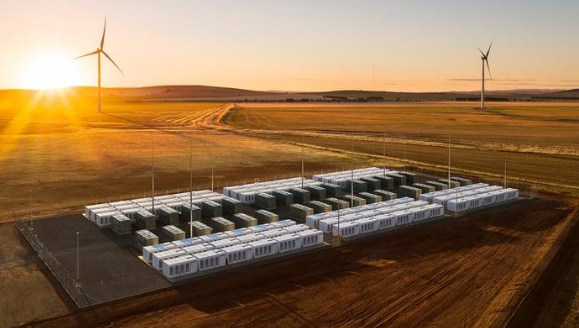
\includegraphics[width=6cm]{figures-Chp0/3-Reseau.png}
\end{minipage}\hfill   
\begin{minipage}[c]{0.35\textwidth}     
\captionof{figure}{Installation d'un centre de stockage d'énergie éolienne, par Tesla, en Australie exploité par le groupe français Neoen [tiré de la \href{https://www.maisondelenergie.fr/sites/maisondelenergie.fr/files/batteries_1.pdf}{maison de l'énergie, batteries}]}
\label{tab:battery_reseau}
\end{minipage}

\`{A} l'heure de la transition écologique, accompagnée du développement des énergies renouvelables, l'intégration des systèmes de stockage de masse au sein des réseaux électriques constitue un enjeu. En effet, les énergies renouvelables : photovoltaïque, éolien, nucléaire sont des sources d'énergies moins flexibles que le charbon ou le gaz. Les deux premières sont intermittentes (c.-à-d. dépendent des conditions environnementales) quand la dernière présente une production constante. Au sein du réseau électrique, l'intégration de batteries permet une meilleure maîtrise des pics ou des déficits de tension électrique.

\begin{comment}
\section{Objectifs du cours}

Il existe de multiples approches pour aborder les batteries, l'une des approches les plus communes est l'approche historique, consistant à décrire les avancées et les développements technologiques autour des batteries. Cette approche est celle utilisée par les chercheurs de renom du domaine comme J.M. Tarascon, professeur au collège de France, qui tient la chaire de Chimie du solide et énergie.

Cependant, cette approche nécessite souvent l'oeil aguéri d'un chimiste accompli dans la maîtrise des outils permettant d'aborder les batteries. Le domaine des matériaux pour l'énergie est un domaine transverse ! Toute la difficulté que vous allez rencontrer sera de faire appel à des notions de : chimie des solutions, de thermodynamique, de physique (électricité/électrostatique) à mettre en relation avec vos connaissances de chimie des matériaux. 

Dans ce cours, le choix a été fait de construire des chapitres/séances autour des "outils" permettant de comprendre cette branche des matériaux, sans aborder les développements technologiques actuels. Les outils développés en cours devront être réinvestis par vous lors des travaux dirigés qui présenteront des exercice de deux natures : 
\begin{enumerate}
\item des applications directes des outils du cours ; 
\item des problèmes plus complexes où vous serez emmené à aborder une technologie ancienne ou actuelle, à l'aide des outils développés en cours.
\end{enumerate}

Lors des séances de travaux pratiques, le choix a été fait de vous faire aborder les concepts élementaires autour des piles et batteries afin de vous familiariser avec les notions élémentaires de ces systèmes, puis de vous faire développer un système plus complexe : une batterie Li-ion, sous forme de "pile bouton".

\section{Organisation des séances}

\`{A} chaque séance, un outil sera abordé de manière théorique et formel. Un polycopié vous sera distribué, abordant le plus souvent le problème de manière conceptualisé et formalisé. Le cours, à l'oral, traitera le plus souvent un exemple type sur la base de laquelle l'outils sera développé et utilisé. Le polycopié et la séance orale sont donc complémentaires et ne peuvent être suivi l'un sans l'autre. Le polycopié est un bon moyen ensuite de revoir les notions abordées dans un cadre général.
\end{comment}

\def \FigPath{/home/jeff/Documents/IUTOrsay/1-Cours/3p06-Cours_Batterie/01-Cours/figures-Chp0/}
\graphicspath{{/home/jeff/Documents/IUTOrsay/1-Cours/3p06-Cours_Batterie/01-Cours/figures-Chp0/}}
\anachapter{Notions élémentaires à usage dans les batteries}
\label{chp:notions_elementaires}


\objectif{

\faBattery[0] Concepts d'oxydo-réduction
\begin{itemize}[label=\faAngleRight]
    \item pile vs accumulateur \& batterie primaire vs secondaire ;
    \item oxydant vs réducteur \& oxydation vs réduction ;
    \item anode vs cathode \& conventions générateur/récepteur ;
    \item potentiel électrique \& potentiel d'électrode ;
    \item tension à courant nul \& force électromotrice ;
    \item composantes d'une cellule : électrodes, électrolyte, séparateur.
\end{itemize}

\faBattery[2] Chimie des batteries
\begin{itemize}[label=\faAngleRight]
	\item réaction de recomposition : formation, déplacement ;
	\item réaction d'insertion : insertion, intercalation, extrusion, topotacticité vs atacticité.
\end{itemize}

\faBattery[4] Connaître les caractéristiques sur l'état ou les performances d'une batterie
\begin{itemize}[label=\faAngleRight]
    \item courant, tension, puissance électrique ;
    \item état de charge et décharge ;
	\item capacité spécifique massique et volumique ;
	\item état de santé ;
	\item énergie théorique maximale ;
	\item qualité énergétique ;
	\item cyclabilité.
\end{itemize}}

\begin{figure}[H]
\centering
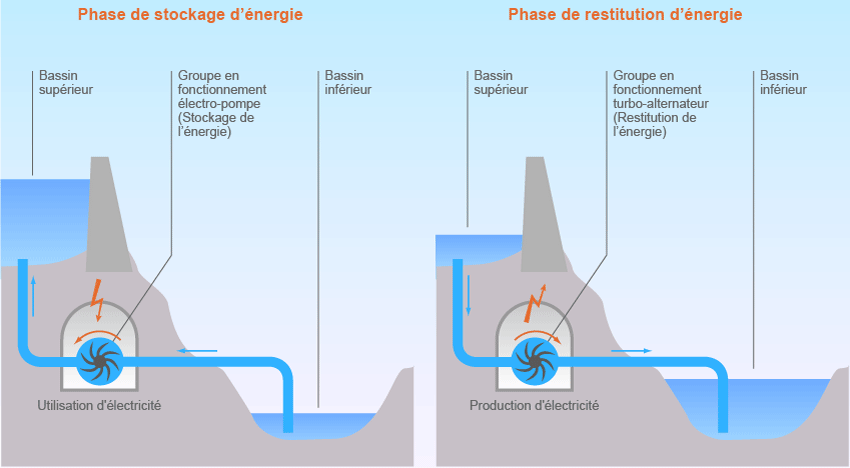
\includegraphics[width=\textwidth]{figures-Chp0/Fig15}
\captionof{figure}{Principe de fonctionnement d'une centrale STEP (Station de Transfert d'\'{E}nergie par Pompage)}
\label{fig:Chp-0-15}
\end{figure}
%https://www.encyclopedie-energie.org/les-stations-de-pompage-step/

Une batterie est un dispositif qui stocke de l'énergie sous forme \blancbis{chimique} et qui le restitue sous forme d'énergie \blancbis{électrique}. En ce sens, on qualifie une batterie de \blancbis{transducteur}\mySideNote{Terme associé à tout dispositif permettant la conversion d'une grandeur physique en une autre.} ou de \blancbis{convertisseur d'énergie}.

De manière assez simple, il est possible d'établir une analogie avec la mécanique. Les stations de transfert d'énergie par pompage, représentées à la Fig. \ref{fig:Chp-0-15}, sont un bon exemple modèle. Lorsque le réseau électrique est en déficit d'énergie électrique, ces stations de haute montagne déversent l'eau du bassin supérieur vers le bassin inférieur. Cette phase correspond à la phase de "décharge" du bassin, où l'énergie potentielle de pesanteur est convertie en énergie électrique. Dans le cas où le réseau est excedentaire en énergie, l'eau du bassin est remontée par un système de pompe. La STEP convertit donc l'énergie électrique en énergie potentielle de pesanteur.


Dans une batterie, un opérateur va mettre en contact deux électrodes\mySideNote{Conducteur électronique (\emph{par ex.} un métal) ou ionique (\emph{par ex.} le verre) captant ou libérant des électrons} où les électrons ont une énergie chimique différente. Lors de cette mise en contact, cette différence d'énergie chimique conduit à la mise en mouvement d'un flux d'électron\mySideNote{Ce flux se manifeste par un courant électrique, noté $I$, qui représente la quantité de charge transporté à travers un conducteur par unité de temps.}. Le flux d'électron conduit petit à petit à un retour à l'équilibre du système.

Lors de ce processus, \blancbis{deux espèces chimiques rédox}, c'est-à-dire des espèces chimiques capables d'\blancbis{échanger un ou plusieurs électrons}, réagissent ensemble. Cette réaction libère de l'énergie sous deux formes : 
\begin{itemize}
    \item un \blancbis{travail utile} \textbf{W'} qui est le travail électrique ;
    \item une \blancbis{déperdition d'énergie}, la chaleur \textbf{Q}, c'est-à-dire de l'énergie thermique.
\end{itemize}

\begin{minipage}[c]{0.65\textwidth}
\centering
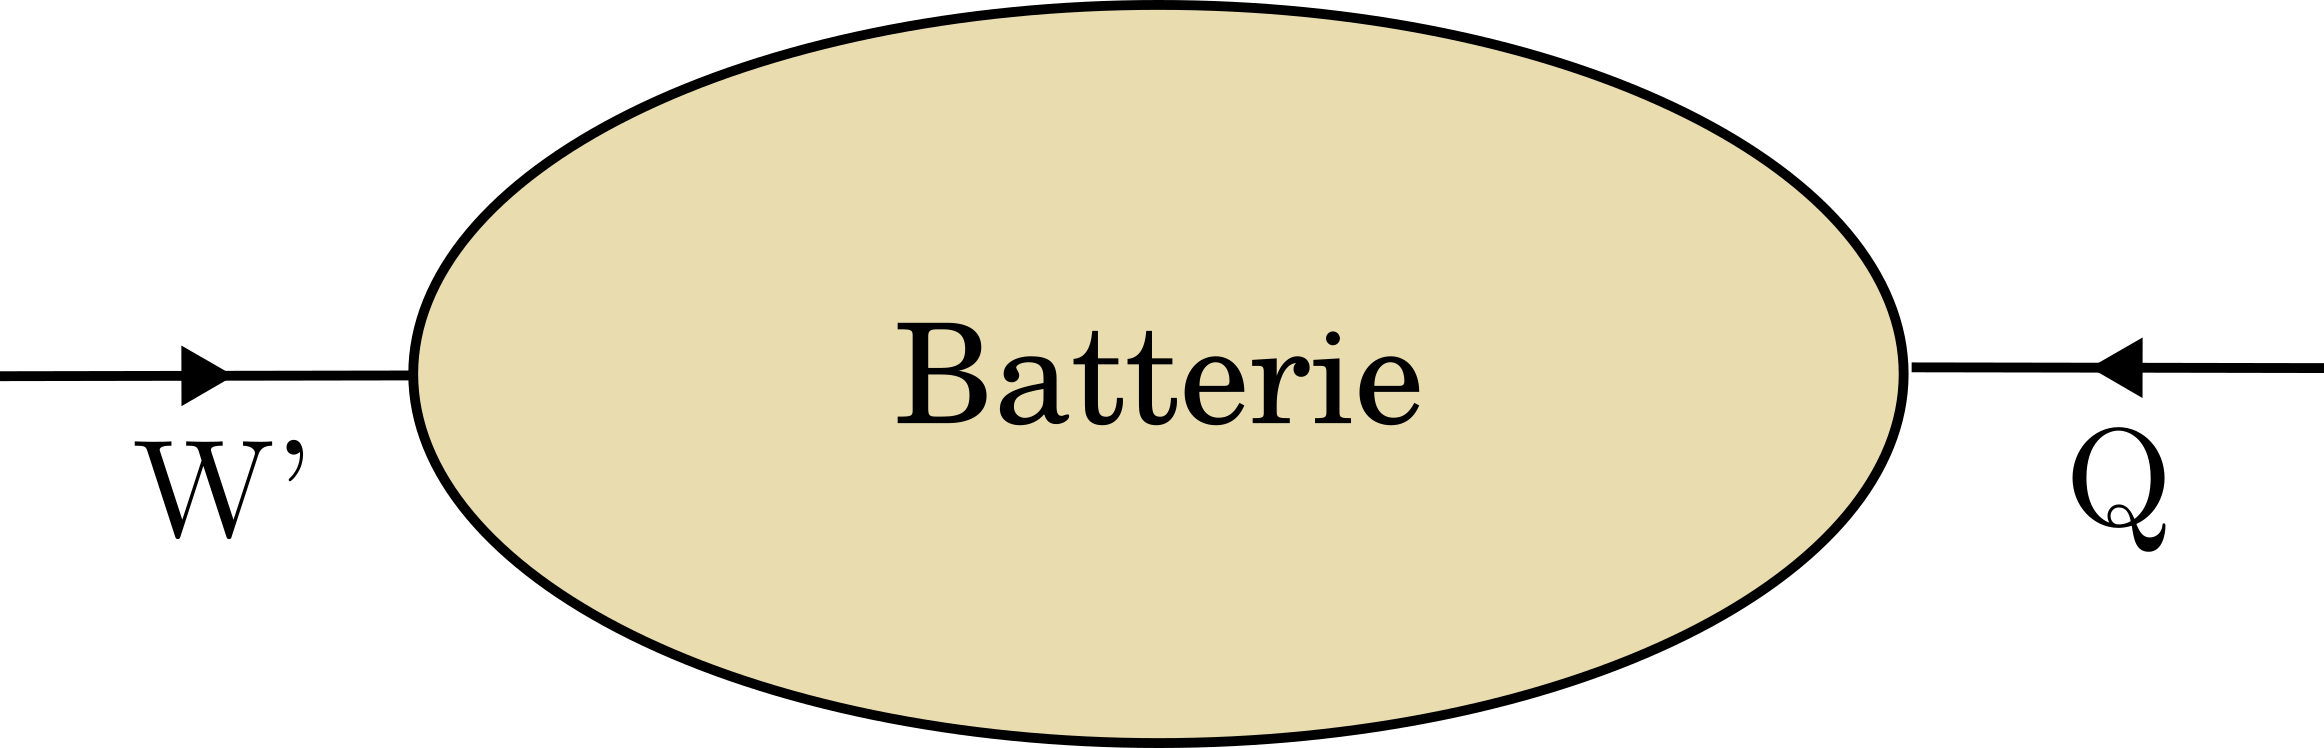
\includegraphics[width=5cm]{figures-Chp0/Fig02.png}
\end{minipage}\hfill   
\begin{minipage}[c]{0.35\textwidth}     
\captionof{figure}{Représentation des flux d'énergie reçus par une batterie.}
\label{fig:Chp-0-02}
\end{minipage}

La batterie est parfois à usage unique ou rechargeable. Ainsi, si la batterie est rechargeable, le travail électrique est soit reçu $W' > 0$ (charge) ou cédé $W' < 0$ (décharge). En son sein, des éléments résistifs imposent que la batterie perd nécessairement, que ça soit en charge ou décharge, une partie de son énergie sous forme thermique $Q < 0$.\mySideNote{\centering
\begin{tabular}{ccc}
& Charge & Décharge \\
$W'$ & $> 0$ & $< 0$\\
$Q$ & $< 0$ & $< 0$ \\
\end{tabular}}

Cette capacité à recevoir ou non du travail électrique permet de classifier les batteries en plusieurs catégories.

\section{Classification des générateurs électrochimiques}

\subsection{Dispositif constitué d'une seule cellule électrochimique}

\begin{figure}[H]
\begin{center}
\begin{tabular}{cc}
\subfloat[\label{fig:03a}]{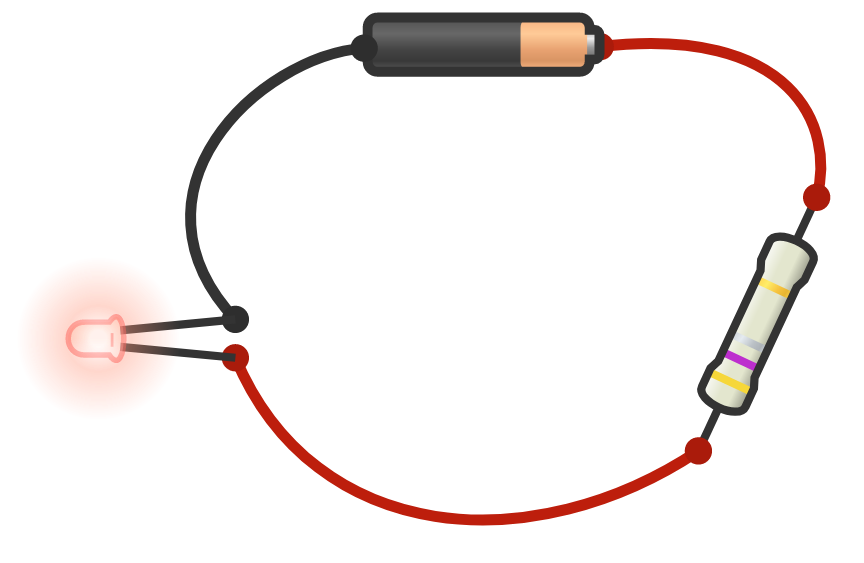
\includegraphics[width=3cm]{figures-Chp0/Fig03a}} & \subfloat[\label{fig:03c}]{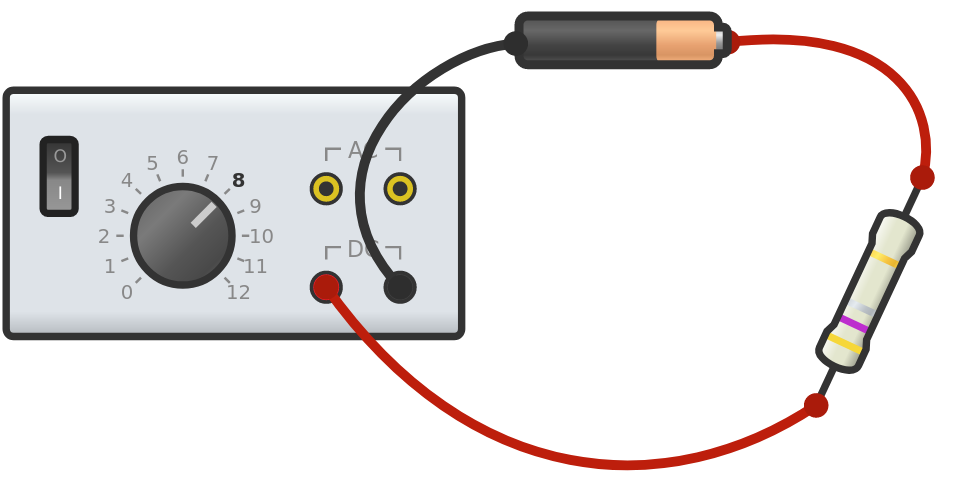
\includegraphics[width=3cm]{figures-Chp0/Fig03c}} \\
\subfloat[\label{fig:03b}]{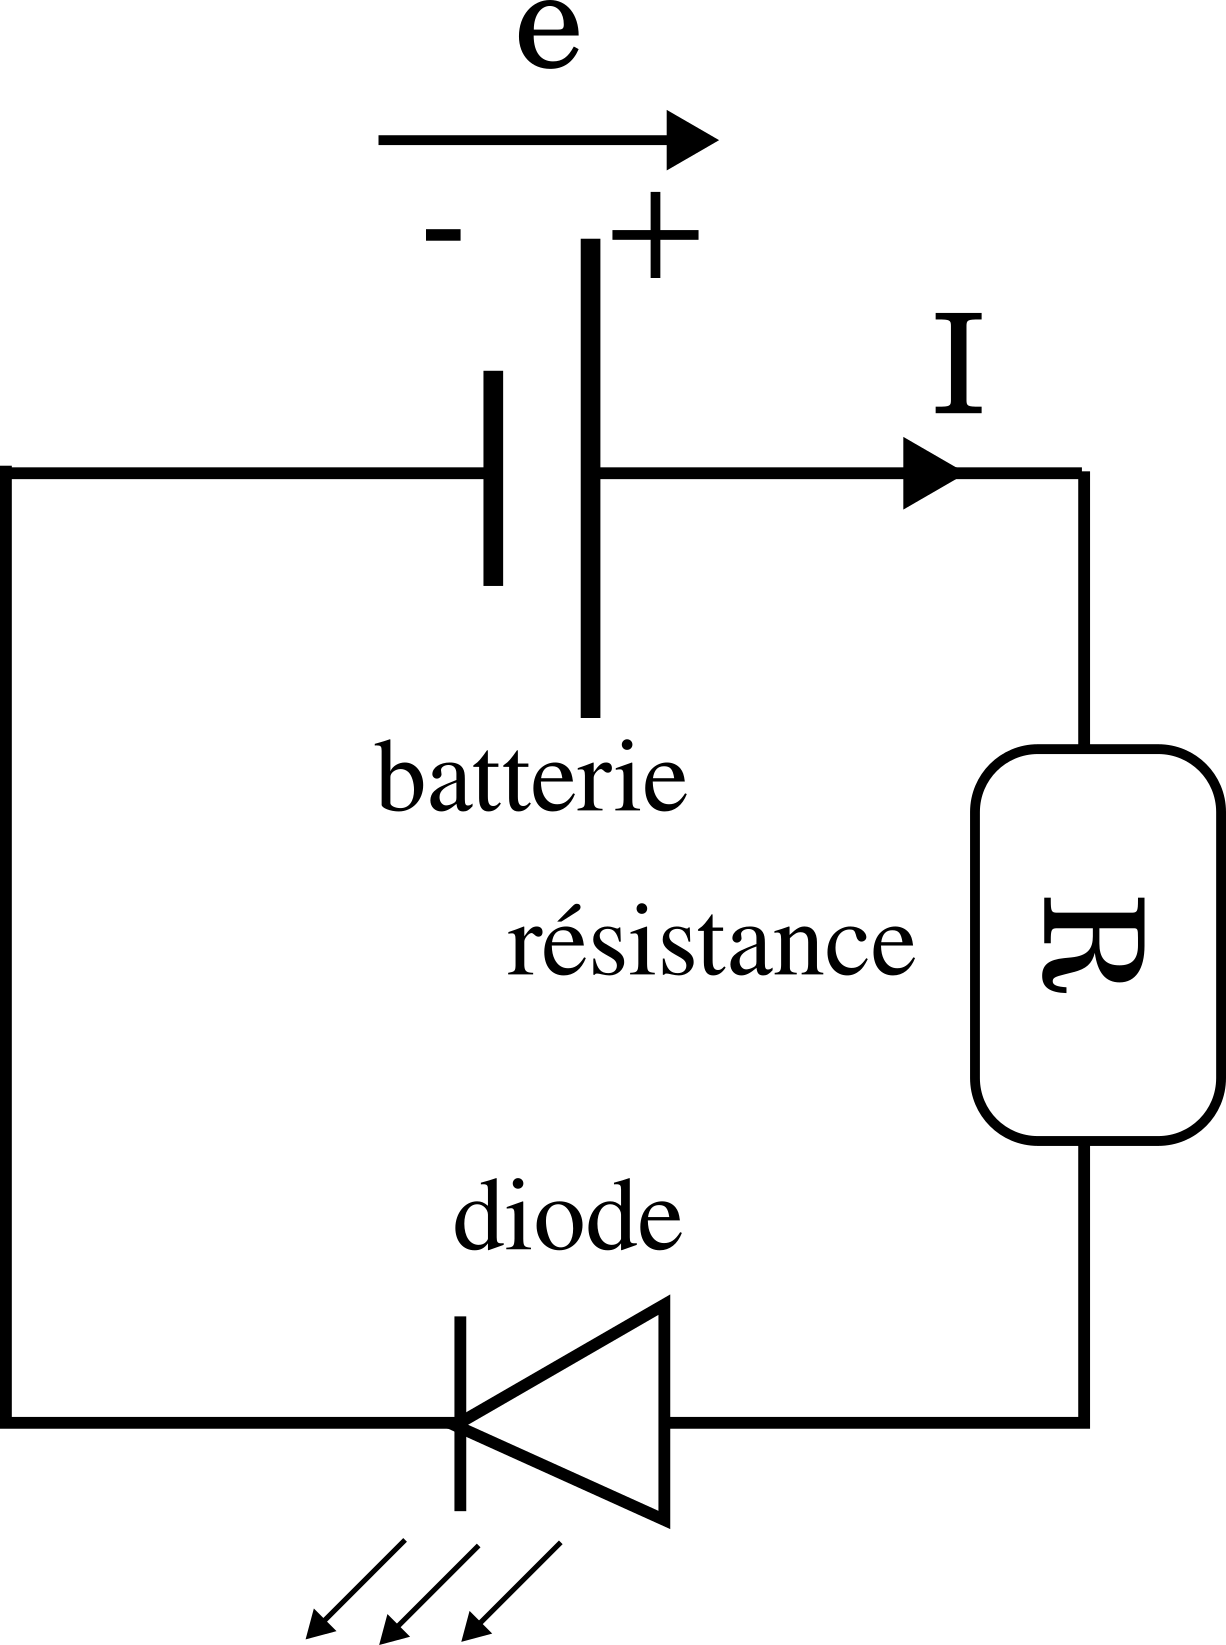
\includegraphics[width=3cm]{figures-Chp0/Fig03b}} & \subfloat[\label{fig:03d}]{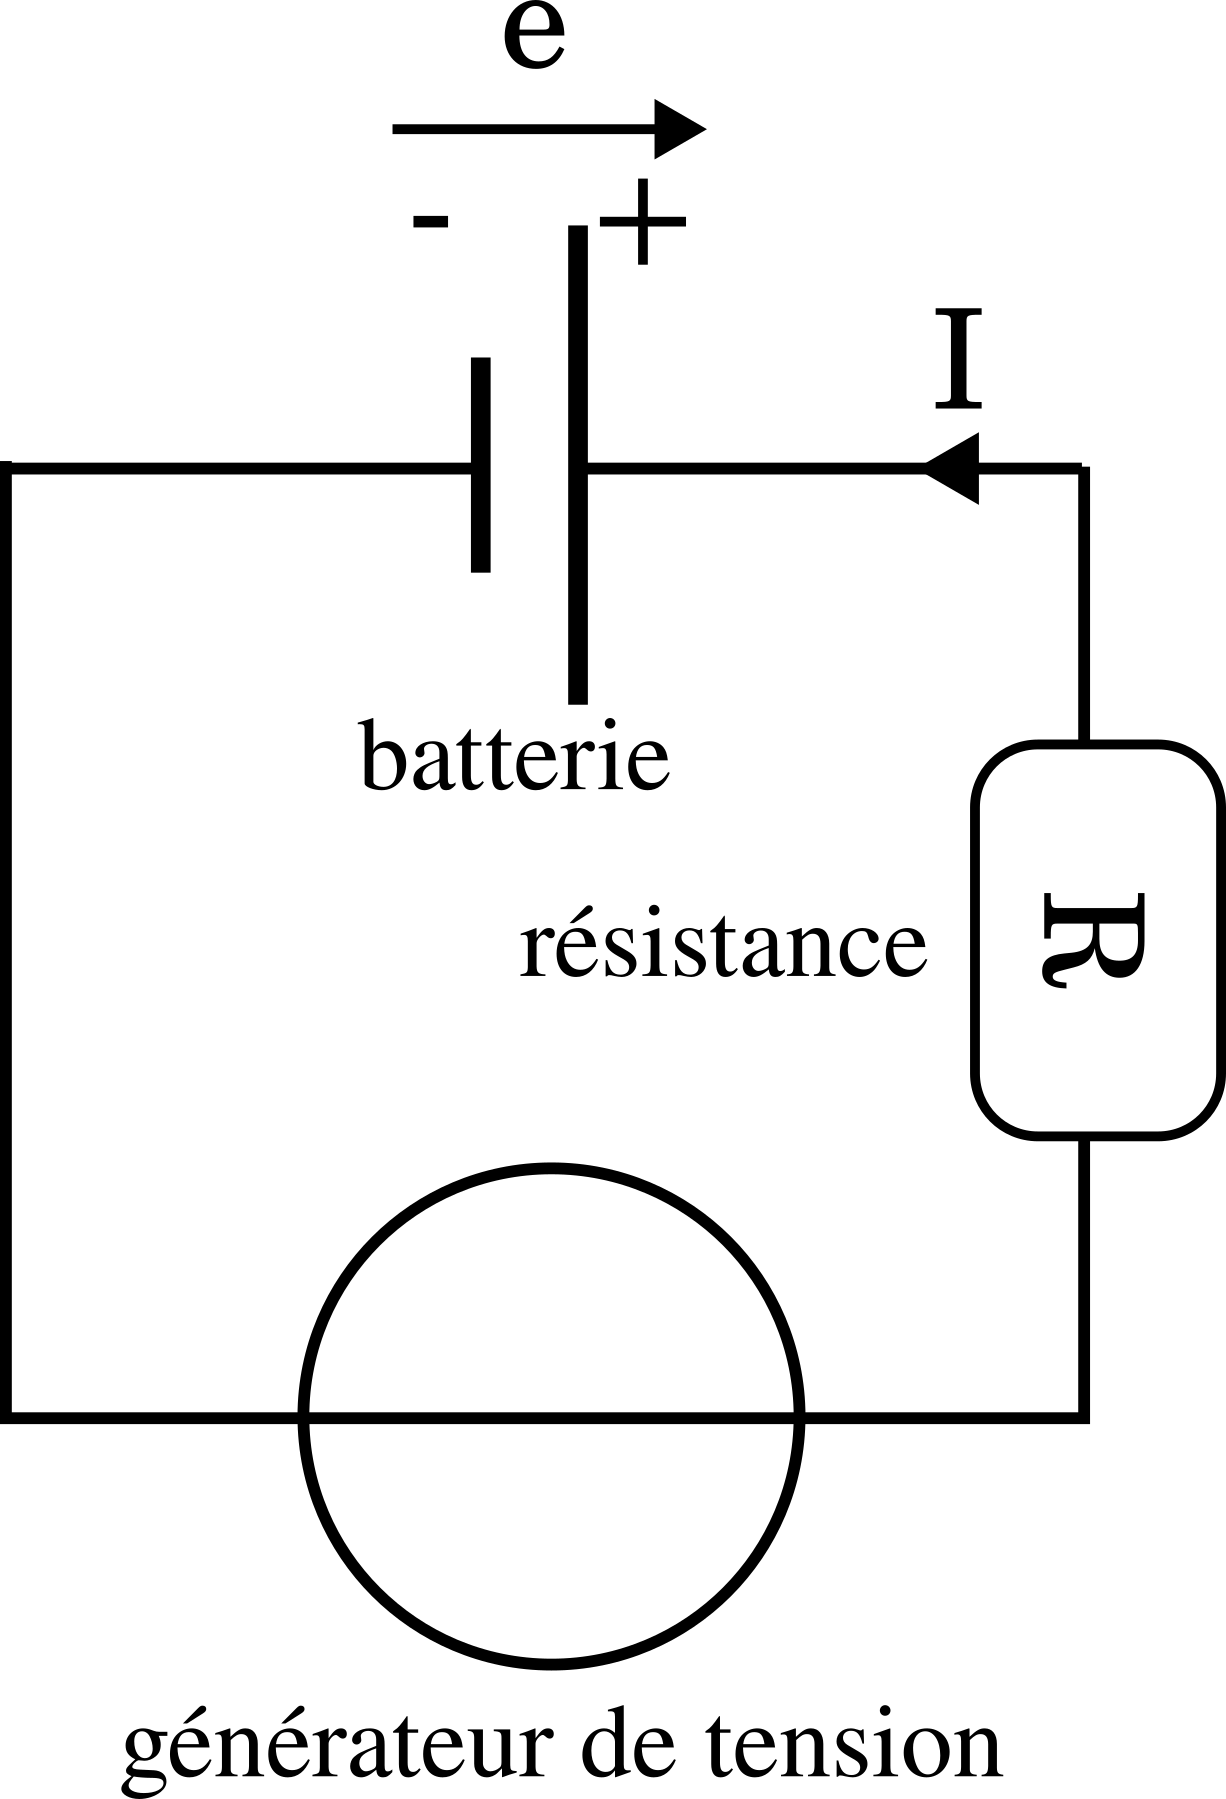
\includegraphics[width=3cm]{figures-Chp0/Fig03d}}
\end{tabular}
\end{center}

%\begin{centering}
%\subfloat[\label{fig:03a}]{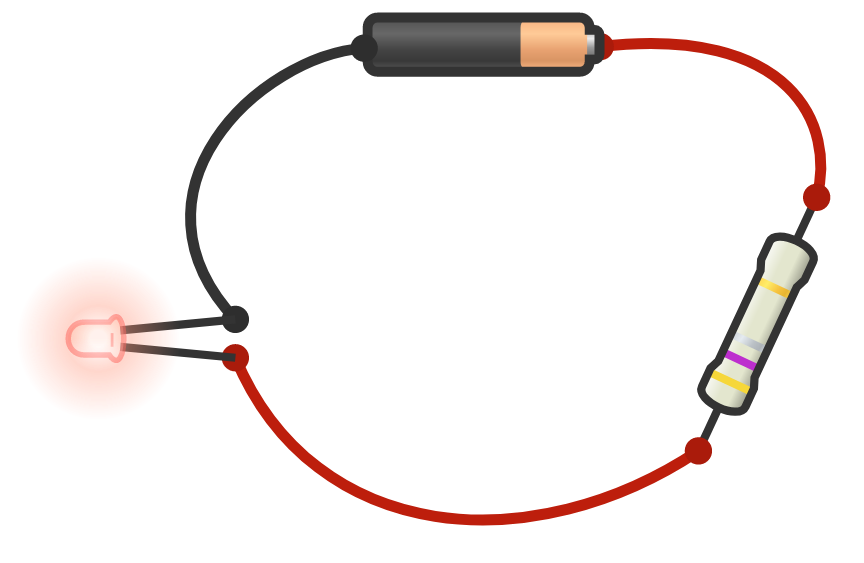
\includegraphics[height=3cm]{figures-Chp0/Fig03a}}\subfloat[\label{fig:03c}]{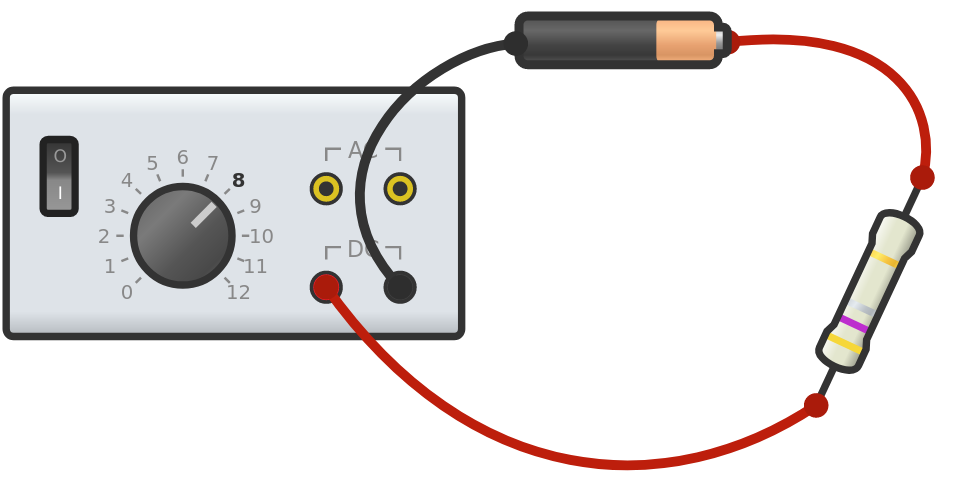
\includegraphics[height=3cm]{figures-Chp0/Fig03c}}\hfill\subfloat[\label{fig:03b}]{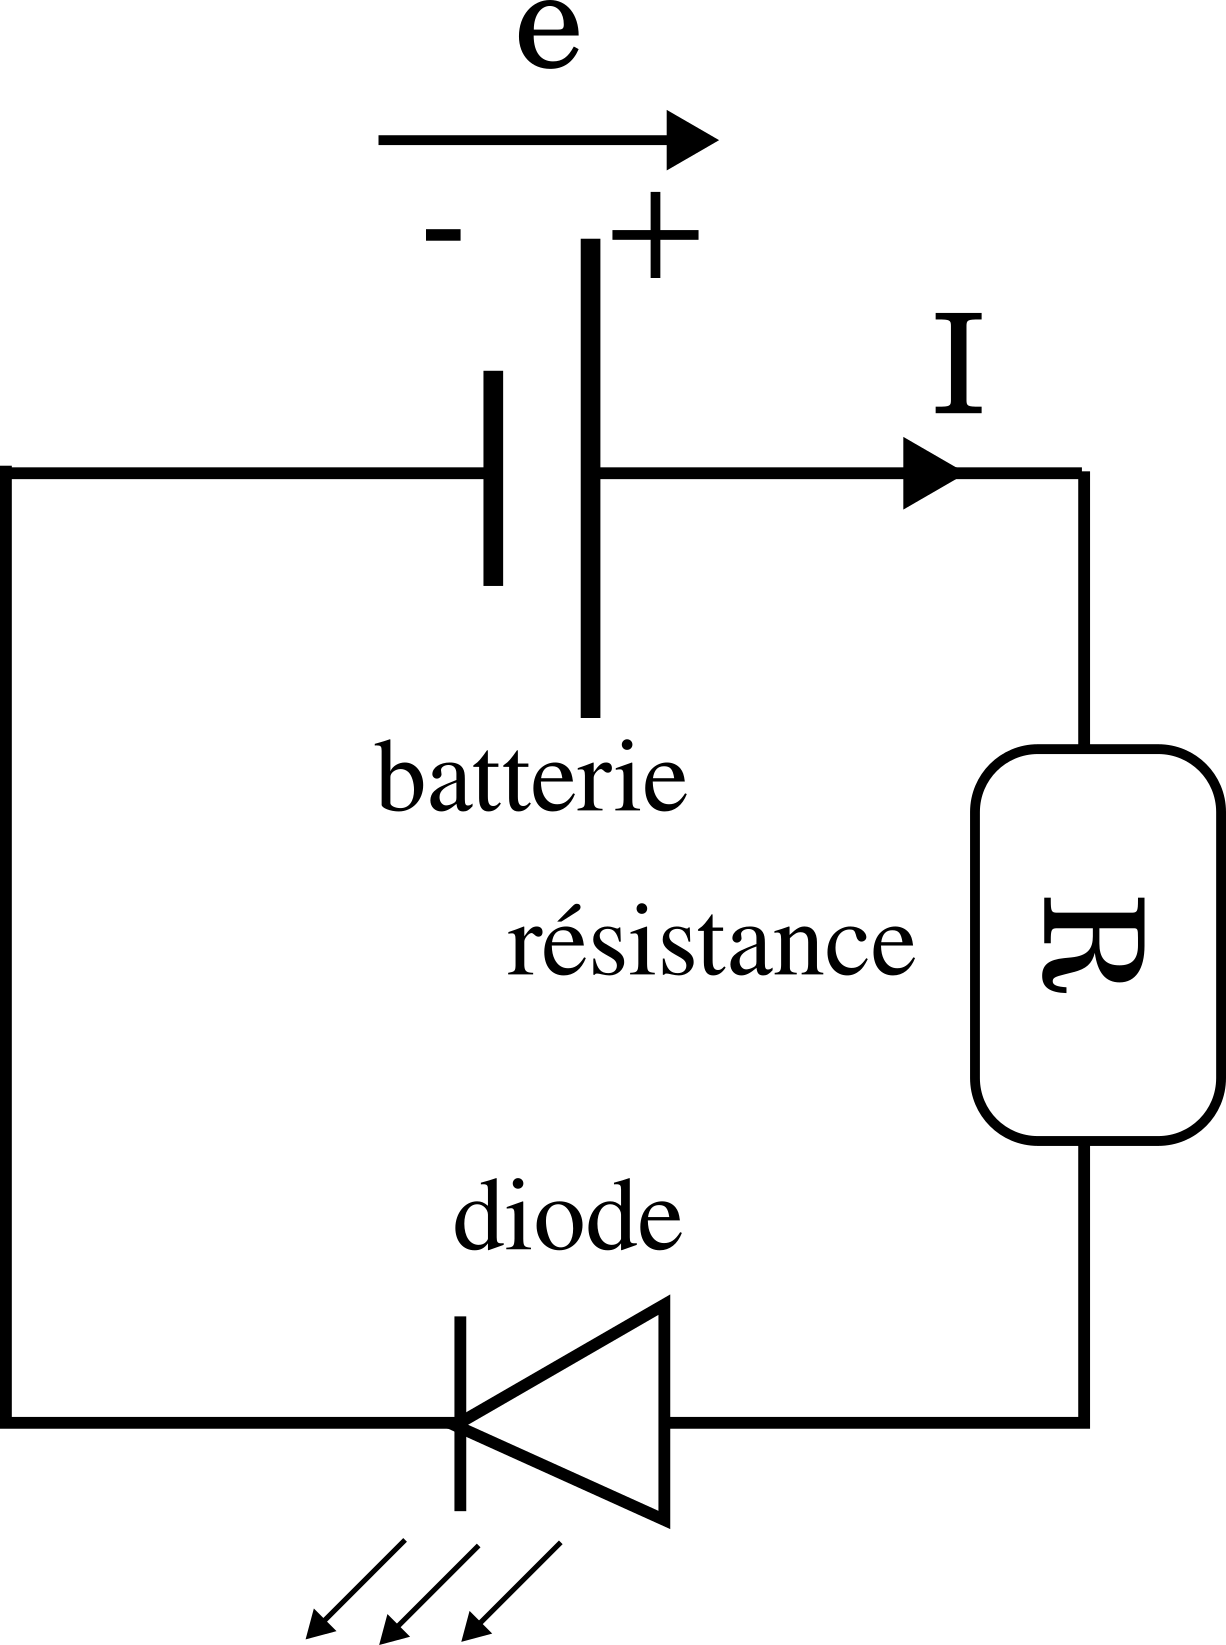
\includegraphics[height=3cm]{figures-Chp0/Fig03b}}\subfloat[\label{fig:03d}]{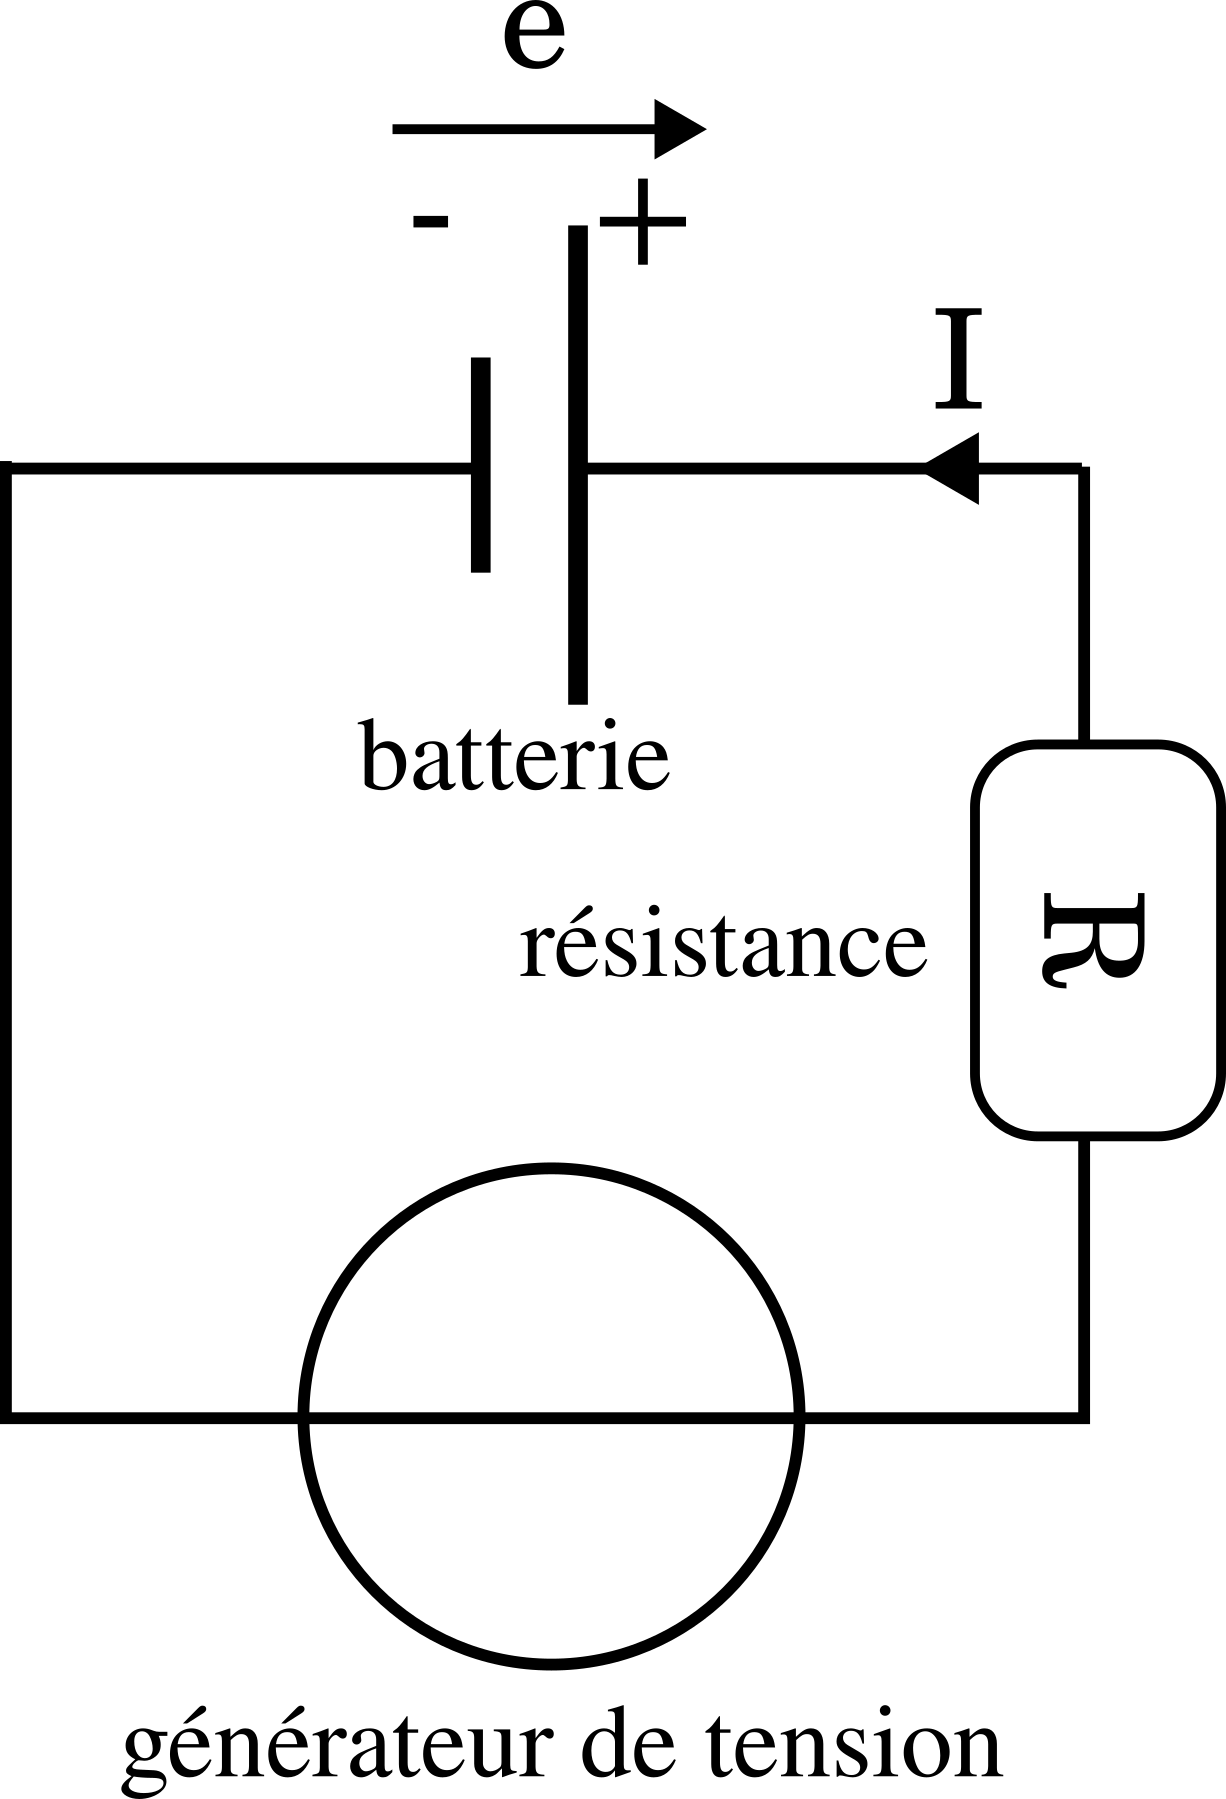
\includegraphics[height=3cm]{figures-Chp0/Fig03d}}
%\par\end{centering}
{\tiny{}\caption{{\small{} Fig. \ref{fig:03a}) Représentation schématique d'une pile AAA alimentant d'une résistance et une diode électroluminescente rouge ; Fig. \ref{fig:03b}) Circuit électrique équivalent ; \ref{fig:03c}) Représentation schématique d'une pile AAA et d'une résistance alimentée par un générateur en mode DC ; Fig. \ref{fig:03d}) Circuit électrique équivalent.}}
}{\tiny\par}
\end{figure}%WARNING : mettre U_B pour la tension de la batterie

\definition{

\blancbis{La pile électrique} est un dispositif électrochimique qui génère de l'électricité en convertissant de l'énergie chimique en énergie électrique grâce à une \blancbis{réaction d'oxydoréduction irréversible}.

~

\blancbis{L'accumulateur} est un dispositif électrochimique qui génère (resp. reçoit) de l'électricité en convertissant de l'énergie chimique (resp. électrique) en énergie électrique (resp. chimique) grâce à \blancbis{une réaction d'oxydoréduction réversible}. 
}

Si la pile AAA, illustré Fig. \ref{fig:03a}/\ref{fig:03b}, peut-être rechargée par le générateur, on peut dire qu'elle est constituée d'accumulateurs. Sinon, elle est constituée de piles.


Du point de vue électrique, l'accumulateur est :
\begin{itemize}
\item un \blancbis{générateur électrique} lorsqu'il se décharge ;
\item un \blancbis{récepteur électrique} lorsqu'il se charge.
\end{itemize}

La pile est quant à elle uniquement un \blancbis{générateur électrique}.


\subsection{Dispositifs constitués de plusieurs cellules électrochimiques}

\blancbis{La batterie} est le nom donné à tout dispositif électrique résultant de la mise en \blancbis{série} et/ou en \blancbis{parallèle}\mySideNote{\`{A} vous de deviner pourquoi une batterie a pour symbôle électrique : 
\begin{center}
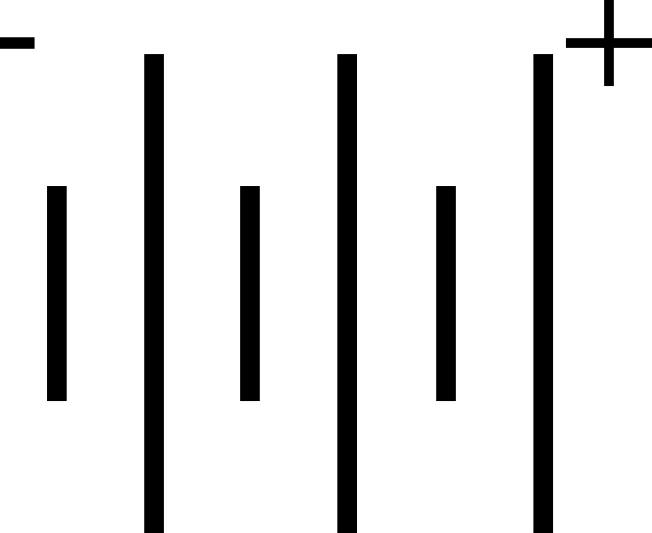
\includegraphics[width=2cm]{figures-Chp0/Fig05}
\end{center}} de plusieurs piles ou accumulateurs. On les classe alors en deux catégories : 
\begin{enumerate}
    \item primaire lorsque l'on a mis en série des piles ;
    \item secondaire lorsqu'on l'on a mis en série des accumulateurs.
\end{enumerate}

Ainsi, tout générateur primaire ne peut être utilisé \blancbis{qu'une seule fois}, et doit être jeté après utilisation. 

\section{Vocabulaire associé aux réactions électrochimiques}
Avant d'aborder les différentes parties d'une batterie, il est important de remettre en place quelques termes de vocabulaire propre aux réactions électrochimiques.

Afin de modéliser le flux d'électron, il est possible de décomposer l'équation de réaction en deux demi-équations rédox\mySideNote{\'{E}quation modélisant la transformation chimique au sein d'un couple rédox} modélisant chacune une \blancbis{oxydation} et une \blancbis{réduction}.

\definition{L'oxydation (resp. la réduction) correspond au processus chimique durant lequel une espèce \blancbis{libère} (resp. \blancbis{capte}) un (ou plusieurs) électron(s).}

Dans le cas d'une pile Daniell, pile impliquant les espèces rédox\mySideNote{On qualifiera de rédox, toute espèce chimique réactive réagissant par transfert d'électron(s). On peut qualifier ces espèces d'électroactives, par opposition aux espèces ne pouvant pas transférer d'électron(s) dites électroinactives.} suivantes : \ce{Cu^{2+}} et \ce{Zn}.

On peut écrire les demi-équations de réactions suivantes :

\begin{center}
\begin{minipage}{0.4\textwidth}
\begin{align*}
    \ce{Cu^{2+} (aq) + 2e^- &= Cu (s)} \\
    \ce{Zn(s) &= Zn^{2+} (aq) + 2e^- } \\
\end{align*}
\end{minipage}    
\end{center}

La première (resp. deuxième) demi-équation rédox correspond à la \blancbis{réduction} (resp. l'\blancbis{oxydation}). La combinaison linéaire de ces deux demi-équations constitue l'équation de réaction\mySideNote{Dans le cas des piles ou des accumulateurs, elle est parfois qualifiée de "fictive" au sens où cette réaction chimique n'a pas lieu dans un unique compartiment.} : 

\begin{align*}
\ce{Cu^{2+} (aq) + Zn(s) &= Cu (s) + Zn^{2+} (aq)}
\end{align*}

Cette réaction est dissymétrique, d'un côté une espèce gagne des électrons, de l'autre une espèce perd des électrons.

\definition{Le \blancbis{réducteur} est l'espèce chimique qui \blancbis{cède} des électrons, tandis que l'\blancbis{oxydant} en \blancbis{gagne}.} 

Dans l'équilibre chimique précédent, on peut identifier l'oxydant et le réducteur :

\begin{align*}
\underbrace{\ce{Cu^{2+}}}_{oxydant} (aq) + \underbrace{\ce{Zn(s)}}_{réducteur} &= \ce{Cu (s)} + \ce{Zn^{2+} (aq)}
\end{align*}

Pour identifier l'espèce qui cède/gagne des électrons, il faut écrire \blancbis{les demi-équations rédox} ou calculer \blancbis{la variation du nombre d'oxydation} des espèces\mySideNote{Le nombre d'oxydation, aussi appelé degré d'oxydation, est une grandeur qui caractérise le déficit d'électron d'un ion par rapport à l'élément chimique neutre.}. On peut donc identifier le couple oxydant/réducteur de deux manières différentes :

\begin{center}
\begin{minipage}[]{5cm}
\centering Demi-équations rédox

\begin{equation*}
\ce{Oxydant + ne^- = Reducteur}
\end{equation*}

\end{minipage}\hspace{0.5cm}\vline\hspace{0.5cm}\begin{minipage}[]{5cm}
\centering Variation du nombre d'oxydation

\begin{align*}
\Delta no (X) > 0 &\implies \text{oxydation} \\
\Delta no (X) < 0 &\implies \text{réduction} \\
\end{align*}

\end{minipage}
\end{center}

\example{
\textbf{Demi-équations rédox}
\begin{center}
\begin{align*}
\ce{Cu^{2+} (aq) + 2e^- &= Cu (s)} \\
\ce{Zn(s) &= Zn^{2+} (aq) + 2e^- }
\end{align*}
\end{center}
\textbf{Nombre d'oxydation}
\begin{align*}
\Delta no(\ce{Cu}) < 0 &\implies \text{réduction du cuivre} \\
&\implies \text{le cuivre est l'oxydant} \\
\Delta no(\ce{Zn}) > 0 &\implies \text{oxydation du zinc} \\
&\implies \text{le zinc est le réducteur}
\end{align*}}

\definition{Deux entités chimiques faisant partie d'une même équation rédox forment un couple rédox, noté le plus souvent par :
\begin{align*}
\text{Oxydant}/\text{Réducteur}
\end{align*}
}

Puisque le flux d'électron est \blancbis{orienté} dans un couple \ce{Ox}/\ce{Red}, il en résulte qu'à l'échelle macroscopique, les batteries forment des dispositifs \blancbis{orientés} électriquement.
\begin{comment}
\exercice{Indiquer les demi-équation rédox et si il s'agit de la modélisation d'une oxydation/réduction sachant que les couples rédox mis en jeux sont les suivants :
\begin{enumerate}
    \item \ce{Li^+ (aq)} / \ce{Li (s)} \& \ce{H2O (l)}/\ce{H2 (g)} ; 
    \item \ce{PbO2} (s) / \ce{Pb^{2+} (aq)} \& \ce{Pb^{2+}} (aq) / \ce{Pb (s)}%voir peut-être retirer SO42-
\end{enumerate}
Dans les réactions suivantes, identifier l'oxydant et le réducteur.

\ce{Li (s) + H2O (l) = Li^+ (aq) + HO^- (aq) + \frac{1}{2} H2 (g)}

\ce{PbO2 (s) + Pb (s) + 2 H2SO4 (aq) = 2PbSO4 (aq) + 2 H2O (l)}
}\end{comment}



\section{Description d'une batterie}
\subsection{Partie électroactive}
La description que nous allons faire traite de manière indifférente les batteries primaires et secondaires. En ces termes, piles et accumulateurs porteront le nom générique de cellule.

Toute cellule est un dispositif composé de $\ldots$

\paragraph*{$\ldots$ deux électrodes} dont l'une sert à capter les électrons et l'autre sert à céder des électrons. Une cellule est, par conséquent, un \textbf{dipôle électrique orienté}, c'est-à-dire composé d'un pôle $\oplus$ et d'un pôle $\ominus$.

La \blancbis{polarisation} électrique\mySideNote{Lorsque l'on parle de polarisation électrique, on sous-entend qu'il existe un pôle $\oplus$/$\ominus$ non confondu.} d'une cellule électrochimique ou batterie est invariante, peu importe le rôle joué au sein d'un circuit électrique.

\`{A} la Fig. \ref{fig:03b}, la batterie joue le rôle de générateur, c'est elle qui va imposer le sens du courant $I$ (donc le sens des électrons). \`{A} la Fig. \ref{fig:03d}, la batterie joue le rôle de récepteur, c'est donc le générateur de tension qui impose la polarisation. Dans les deux cas, les pôles de la batterie sont inchangés\mySideNote{Dans un générateur (resp. récepteur) électrique, le courant sort (resp. entre) par le pôle $\oplus$}. 

Le pôle, concept purement électrique, ne donne aucune information apparente sur la chimie au sein des demi-piles. On oriente chimiquement la batterie à l'aide des termes \blancbis{cathode}/\blancbis{anode}.

\definition{En décharge, le pôle $\oplus$ (resp. $\ominus$) d'une batterie est qualifié de \blancbis{cathode} (resp. \blancbis{anode}) lorsqu'il est le siège d'une réaction de \blancbis{réduction} (resp. d'\blancbis{oxydation}).}

Il existe une juste correspondance entre les termes électrique et les phénomènes chimiques ayant lieu, qui est résumé à la Tab. \ref{tab:Chp-0-conventions}.

\begin{center}
\begin{tabular}{|C{2.5cm}|C{3cm}|C{2cm}|C{2cm}|}
\hline
& & \multicolumn{2}{c|}{Polarisation électrique} \\
\hline
& & $\ominus$ & $\oplus$ \\
\hline
\multirow{2}{*}{Rôle électrique} & Générateur & anode & cathode \\
& Récepteur & cathode & anode \\
\hline
\end{tabular}
\captionof{table}{Relation entre électricité et chimie dans une cellule électrochimique ou une batterie.}
\label{tab:Chp-0-conventions}
\end{center}
%Rôle joué par la cellule dans le circuit

\attention{
Par abus de langage, les chimistes portant peu d'intérêt au rôle de la batterie au sein d'un circuit électrique utilise le terme anode (resp. cathode) en parlant du pôle $\ominus$ (resp. anode) en prenant comme référence la cellule ou batterie en décharge.\\

Il va de soi, qu'en toute rigueur, il faut nommer la demi-pile par ses pôles (puisque c'est l'invariant).
}


\subsection{Partie électroinactive}

Dans le cas d'une pile Daniell, pile utilisant les couples \ce{Cu^{2+}(aq)}/\ce{Cu(s)} et \ce{Zn^{2+}(aq)}/\ce{Zn(s)}, le dispositif peut se présenter de la manière suivante :

\begin{minipage}[c]{0.65\textwidth}
\centering
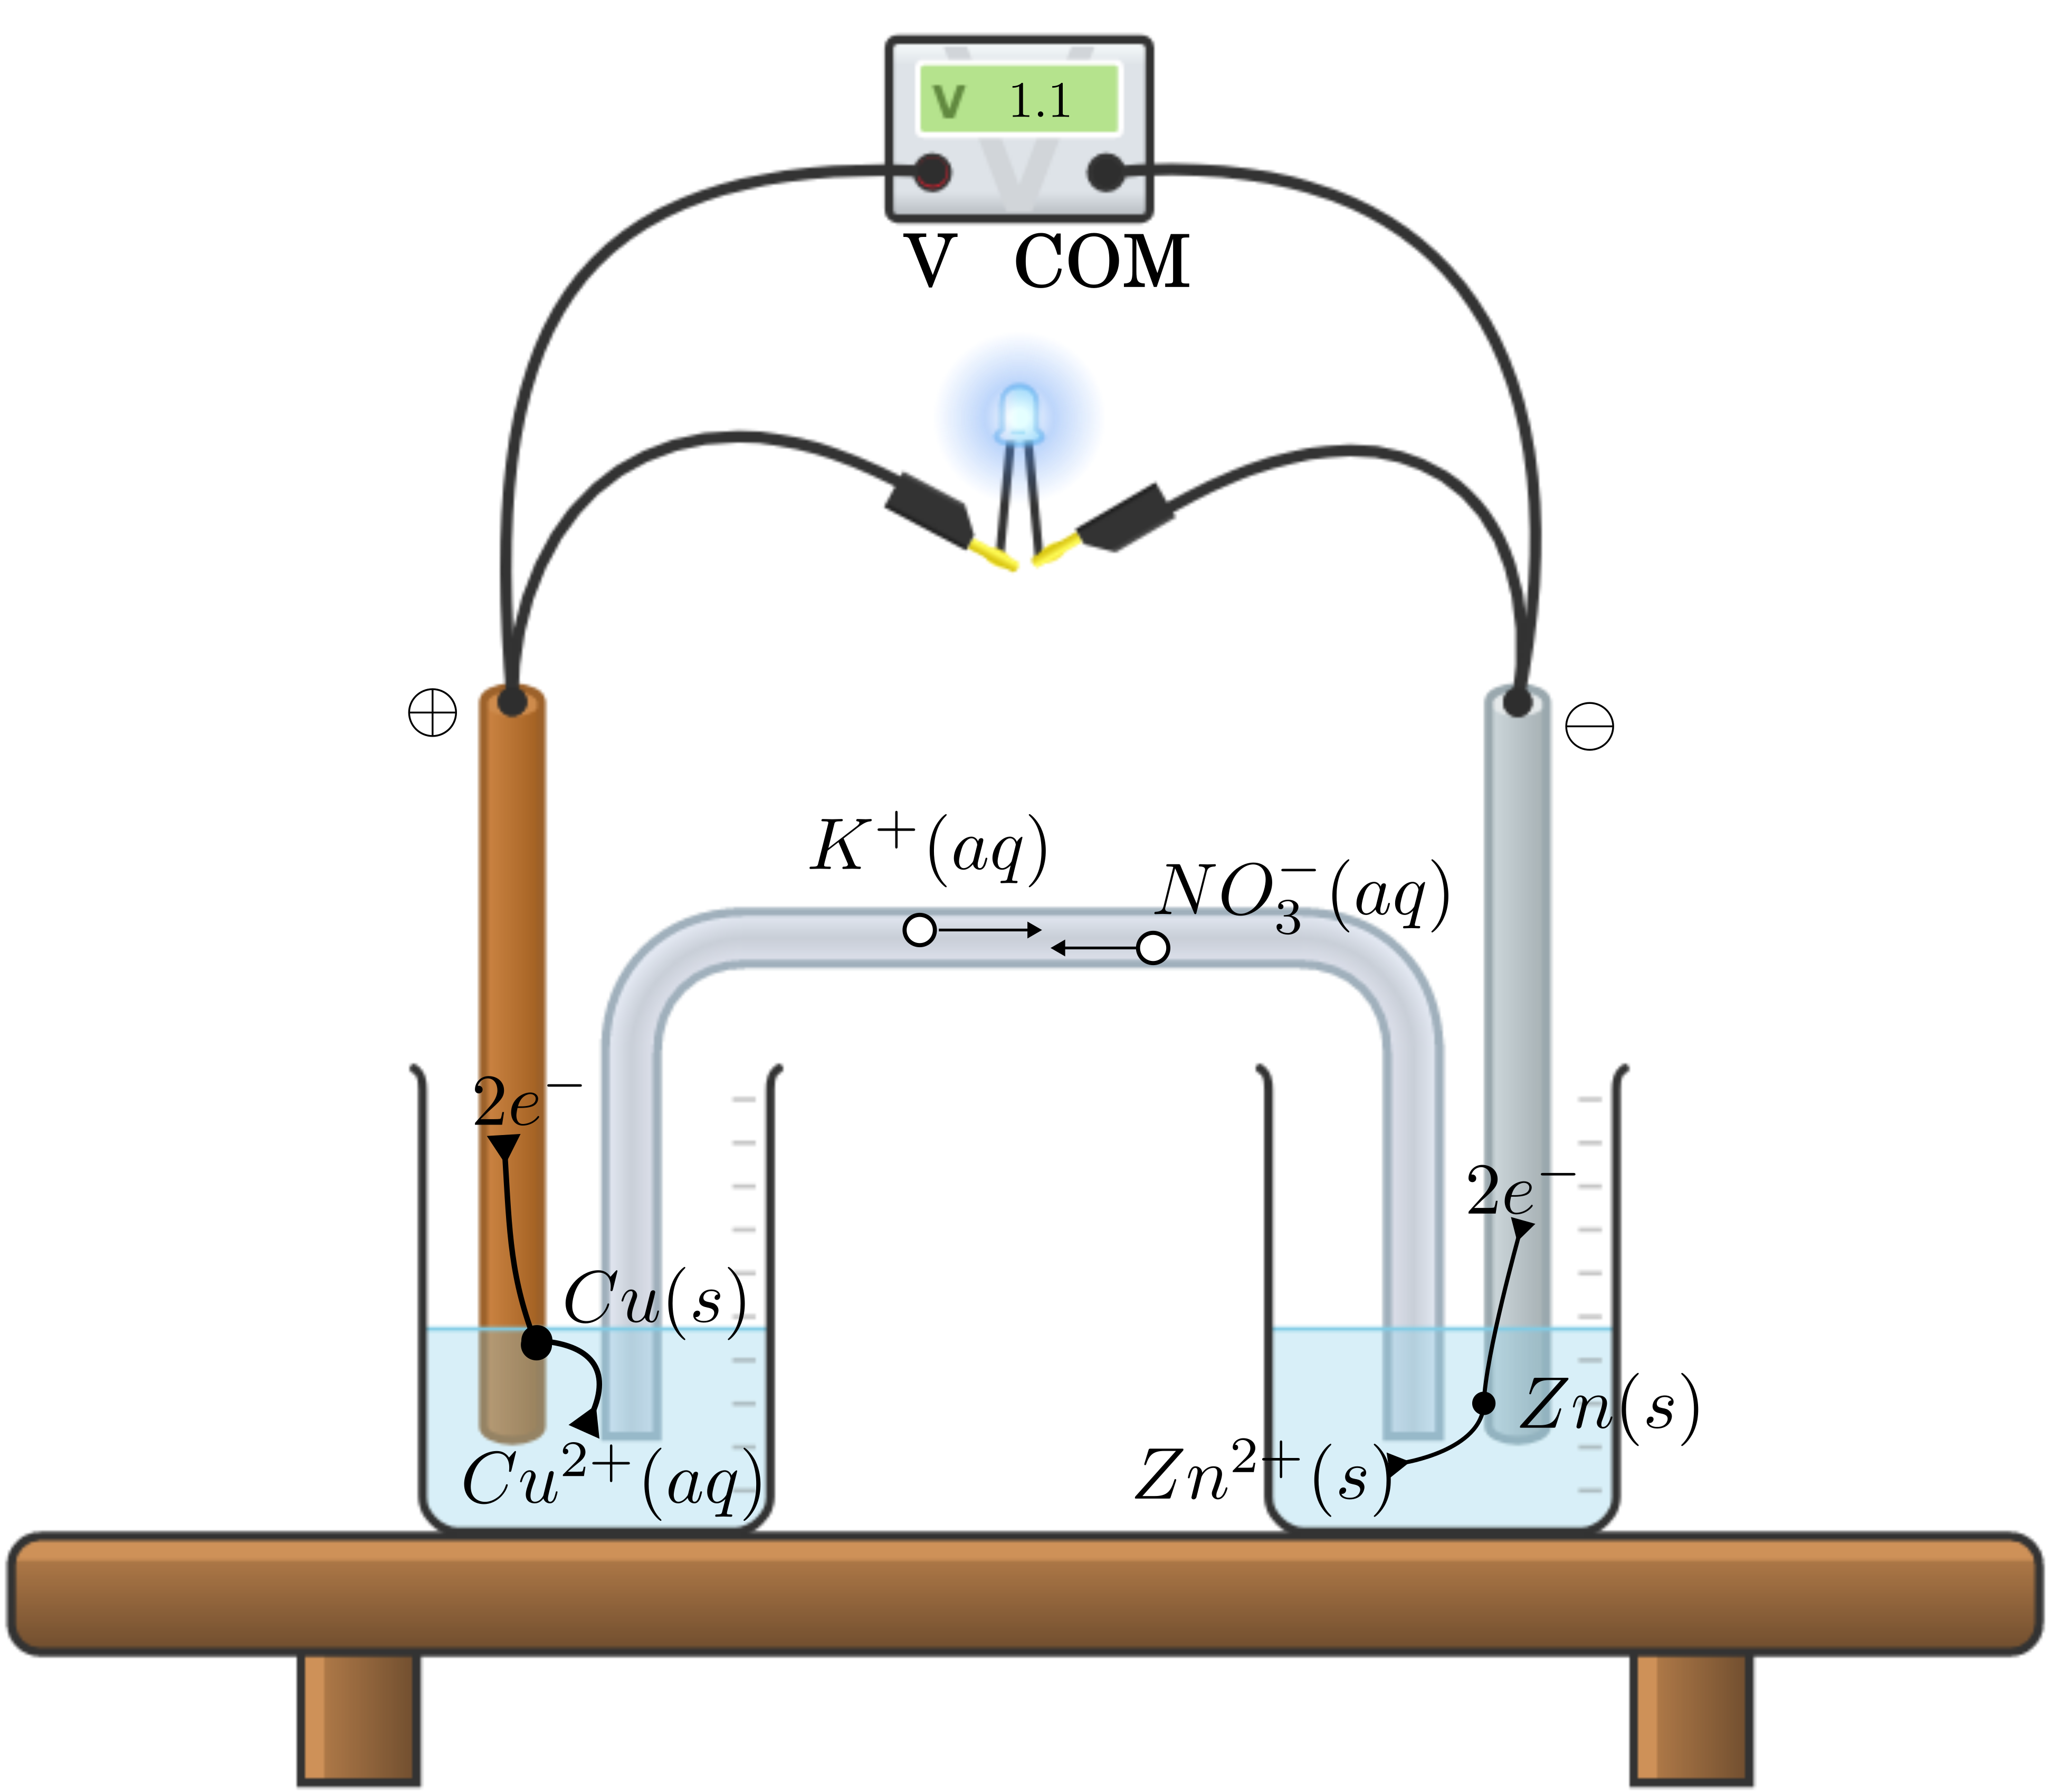
\includegraphics[width=8cm]{figures-Chp0/Fig04.png}
\end{minipage}\hfill   
\begin{minipage}[c]{0.35\textwidth}     
\captionof{figure}{Pile Daniell réalisée à l'aide :}
\begin{itemize}
    \item d'une solution de sulfate de cuivre accompagné d'une plaque de cuivre (cathode) ;
    \item d'une solution de sulfate de zinc accompagné d'une plaque de zinc (anode).
\end{itemize}
\label{fig:04}
\end{minipage}

Le dispositif peut se résumer de la manière suivante : 
\begin{equation*}
\ominus \quad \ce{Zn(s)} | \ce{Zn^{2+} (aq)}; \ce{SO_4^{2-} (aq)} | K^+ (aq), NO_3^- (aq) | \ce{Cu^{2+} (aq)}; \ce{SO_4^{2-} (aq)} | \ce{Cu(s)} \quad \oplus
\end{equation*}
en indiquant par $|$ les interfaces entre les différentes phases.


Une des premières choses à remarquer est que les fils électriques permettent de fermer le circuit électrique, tandis que le pont salin contenant une solution de \ce{KNO3} concentrée permet de fermer la partie chimique. Si le circuit n'est pas fermé dans la partie chimique ou la partie électrique, un ampèremètre branché aux bornes de la cellule indiquera un courant nul\mySideNote{Ceci n'est qu'un constat expérimental qui servira de généralisation. En réalité, il est tout à fait possible de démontrer cette observation grâce aux lois de l'électrostatique.}.

%\mySideNote{La migration est le terme associé à la mise en mouvement d'une particule chargée sous l'action d'un champ électrique. Ce terme est à mettre en perspective avec la diffusion et la convection. Ces phénomènes, dit de transport, seront traité en S4.06.}

\definition{
\blancbis{Solvant} ~  Il s'agit de l'espèce permettant de \blancbis{solvater} les espèces rédox et électrolytiques.

~

\blancbis{Electrolyte} ~  Afin de fermer le circuit électrique et permettre la circulation des électrons, le courant doit pouvoir circuler dans la cellule. Contrairement aux fils et électrodes, où le courant est assuré par les électrons, dans la solution et le séparateur, le courant est assuré par la \blancbis{migration} des ions.

Celui-ci est choisi en fonction de deux contraintes : 
\begin{enumerate}
    \item diminuer la résistivité des compartiments anodiques et cathodiques ;
    \item garantir le processus de migration au sein de la solution.
\end{enumerate}

~

\blancbis{Séparateur} ~  En général, les cellules sont composées d'un séparateur qui permet de séparer \blancbis{physiquement} et \blancbis{spécifiquement} les espèces électroactives du compartiment anodique et cathodique. Le séparateur est soit une membrane, soit un pont salin. Ce séparateur obéit à deux contraintes : empêcher toute réaction parasite entre espèces électroactives, tout en assurant une bonne conductivité ionique d'espèces chimiques chargées, mais inertes chimiquement.
}

L'ensemble chimique électrolyte, solvant et séparateur, qualifié d'\blancbis{électroinactif}, joue un rôle clef dans le fonctionnement d'une batterie/pile mais ne sera quasiment jamais abordé dans ce module où on s'intéressera avant tout au design de la partie électroactive.\mySideNote{L'électrolyte support est parfois une (ou des espèces) électroactive(s), comme dans le cas de la pile Daniell.} En général, on se limitera à écrire les espèces électroactives : 

\begin{equation*}
\ominus \quad \ce{Zn(s)} | \ce{Zn^{2+} (aq)} || \ce{Cu^{2+} (aq)} | \ce{Cu(s)} \quad \oplus
\end{equation*}

Sauf si on a besoin des autres espèces pour comprendre le problème physique.

\subsection{Batterie, tension électrique et force électromotrice}

\begin{figure}[H]
\begin{center}
\begin{tabular}{cc}
\subfloat[\label{fig:Chp0-16a}]{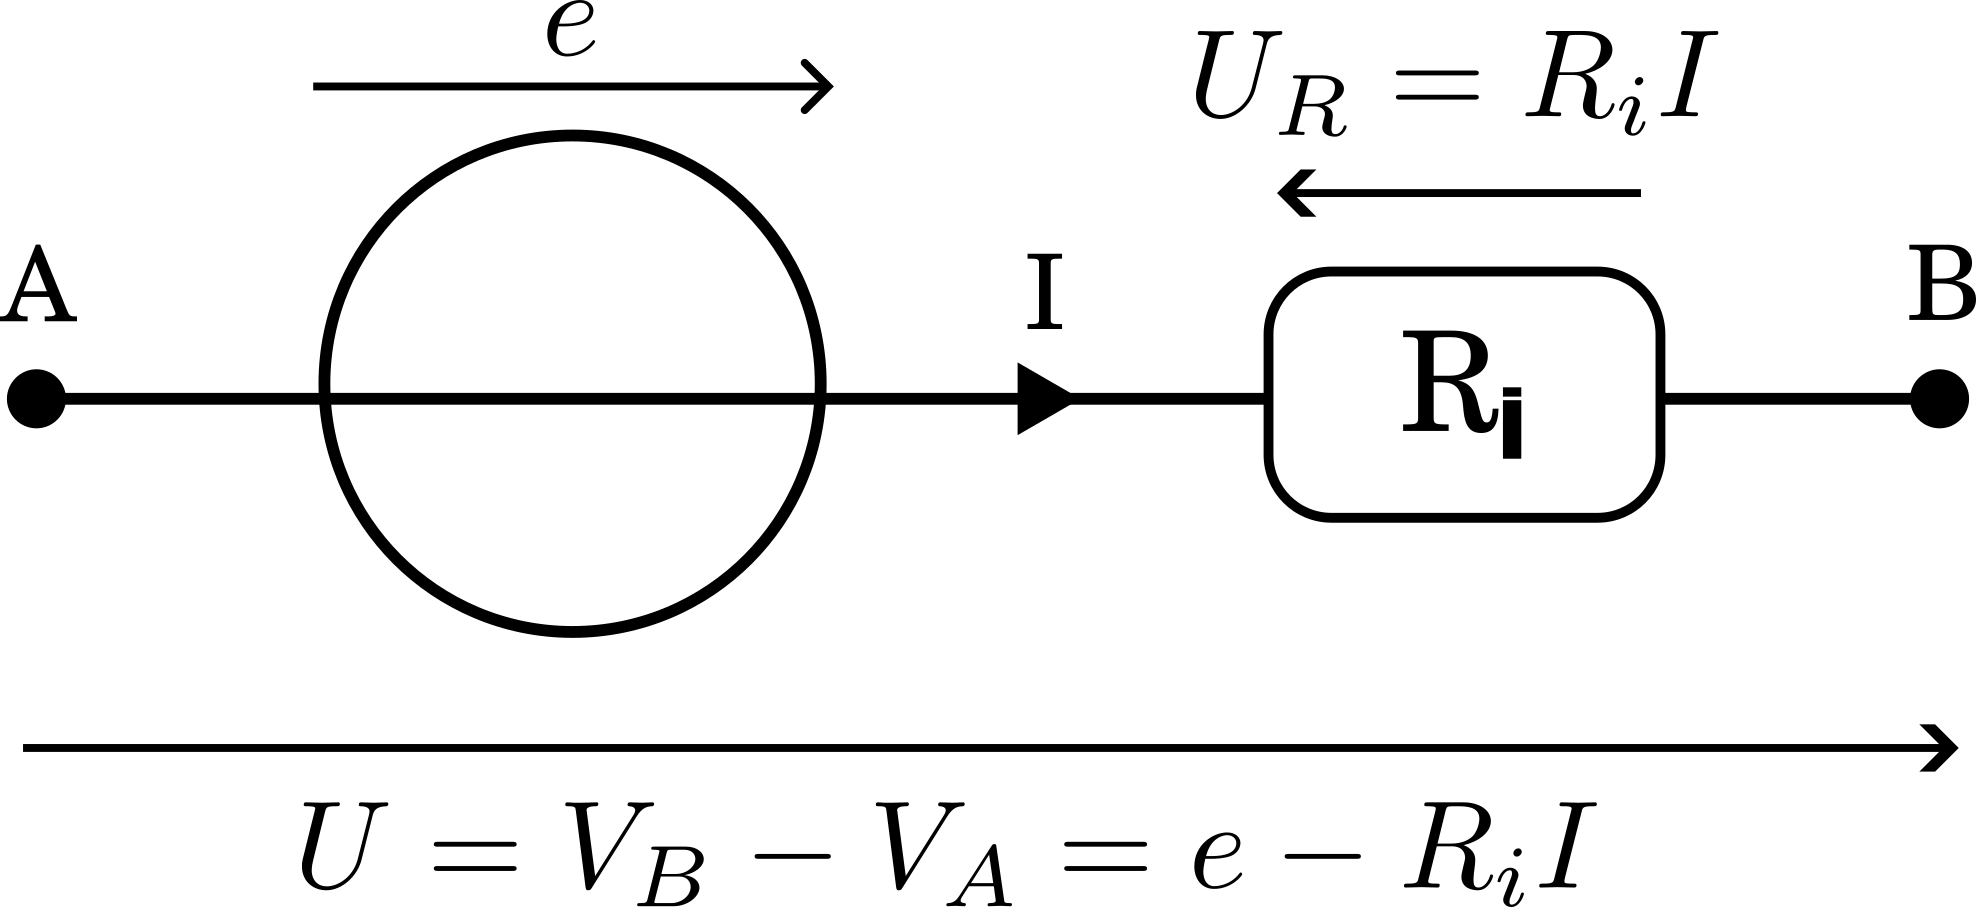
\includegraphics[width=0.48\textwidth]{figures-Chp0/Fig16a}} & \subfloat[\label{fig:Chp0-16b}]{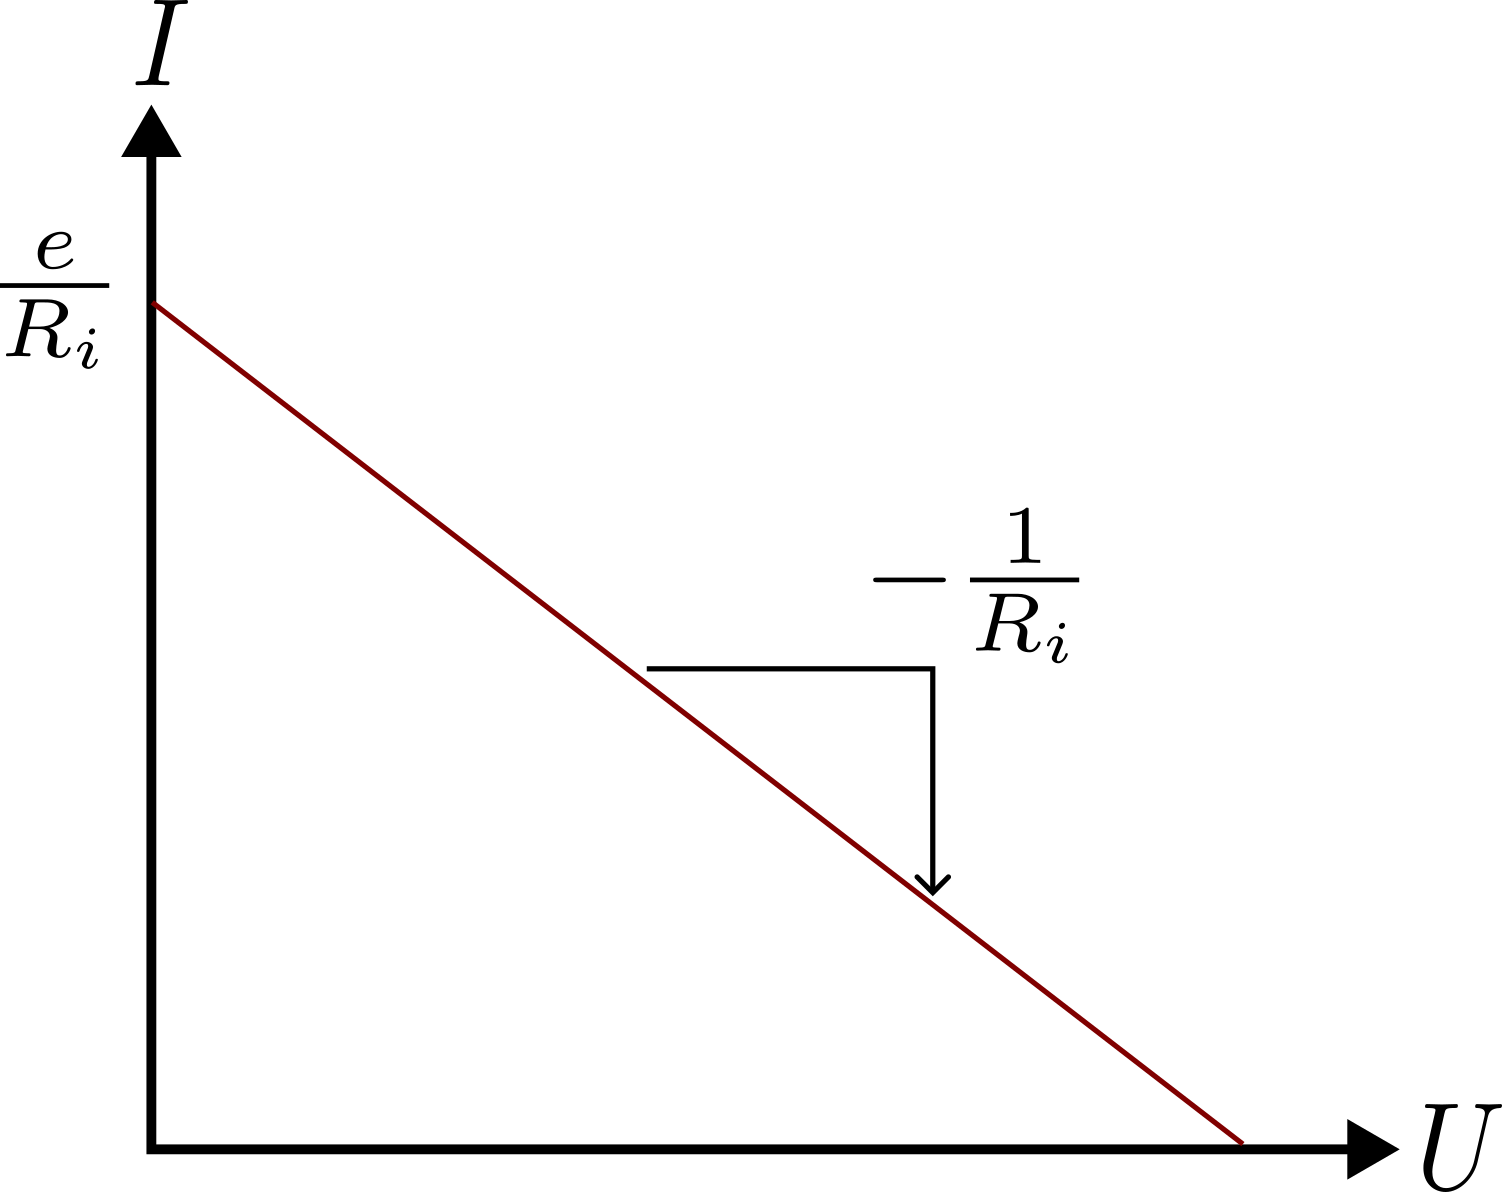
\includegraphics[width=0.30\textwidth]{figures-Chp0/Fig16b}}
\end{tabular}
\end{center}
\caption{\ref{fig:Chp0-16a} Modèle de Thévenin permettant la description de la caractéristique d'une cellule électrochimique ; \ref{fig:Chp0-16b} Allure de la caractéristique d'une cellule électrochimique}
\end{figure}

Lorsque l'on mesure la tension aux bornes d'une cellule électrochimique, notée $U$, on mesure une différence de potentiel électrique entre les deux pôles de la pile. Cette tension électrique dépend de deux paramètres électriques comme représenté à la Fig. \ref{fig:04} :\mySideNote{Ces grandeurs ont été vu en Physique en S1.} 
\begin{itemize}
\item la \blancbis{tension à courant nul}, souvent appelée tension de circuit ouvert\mySideNote{On la rencontrera en TP sous le terme OCV pour \textbf{Open-circuit voltage}.} ;
\item la \blancbis{résistance interne}, notée $R_i$, de la cellule.%inclu résistance de polarisation
\end{itemize}

L'origine chimique de ce comportement pourra être expliqué à la suite d'un cours intensif de thermodynamique et de cinétique électrochimique et sera admis comme tel pour le moment.

Dans les études que nous allons faire sur les batteries, nous chercherons avant tout à établir un lien structure/propriété entre la \emph{tension à courant nul} et la structure chimique aux électrodes. En effet, la tension à courant nul est associée à une grandeur thermodynamique, appelée force électromotrice et notée $e$ qui quantifie la force électrique permettant de séparer les charges au sein de la batterie



\example{
Le voltmètre dispose d'une très grande résistance (idéal = résistance infinie), on va donc bien mesurer la tension à courant nul. De plus, si les électrodes sont des phases homogènes et isotropes macroscopiquement, le potentiel électrostatique est constant. On va pouvoir décomposer le potentiel électrique en fonction des différents points dans la batterie schématisée à la Fig. 

\begin{center}
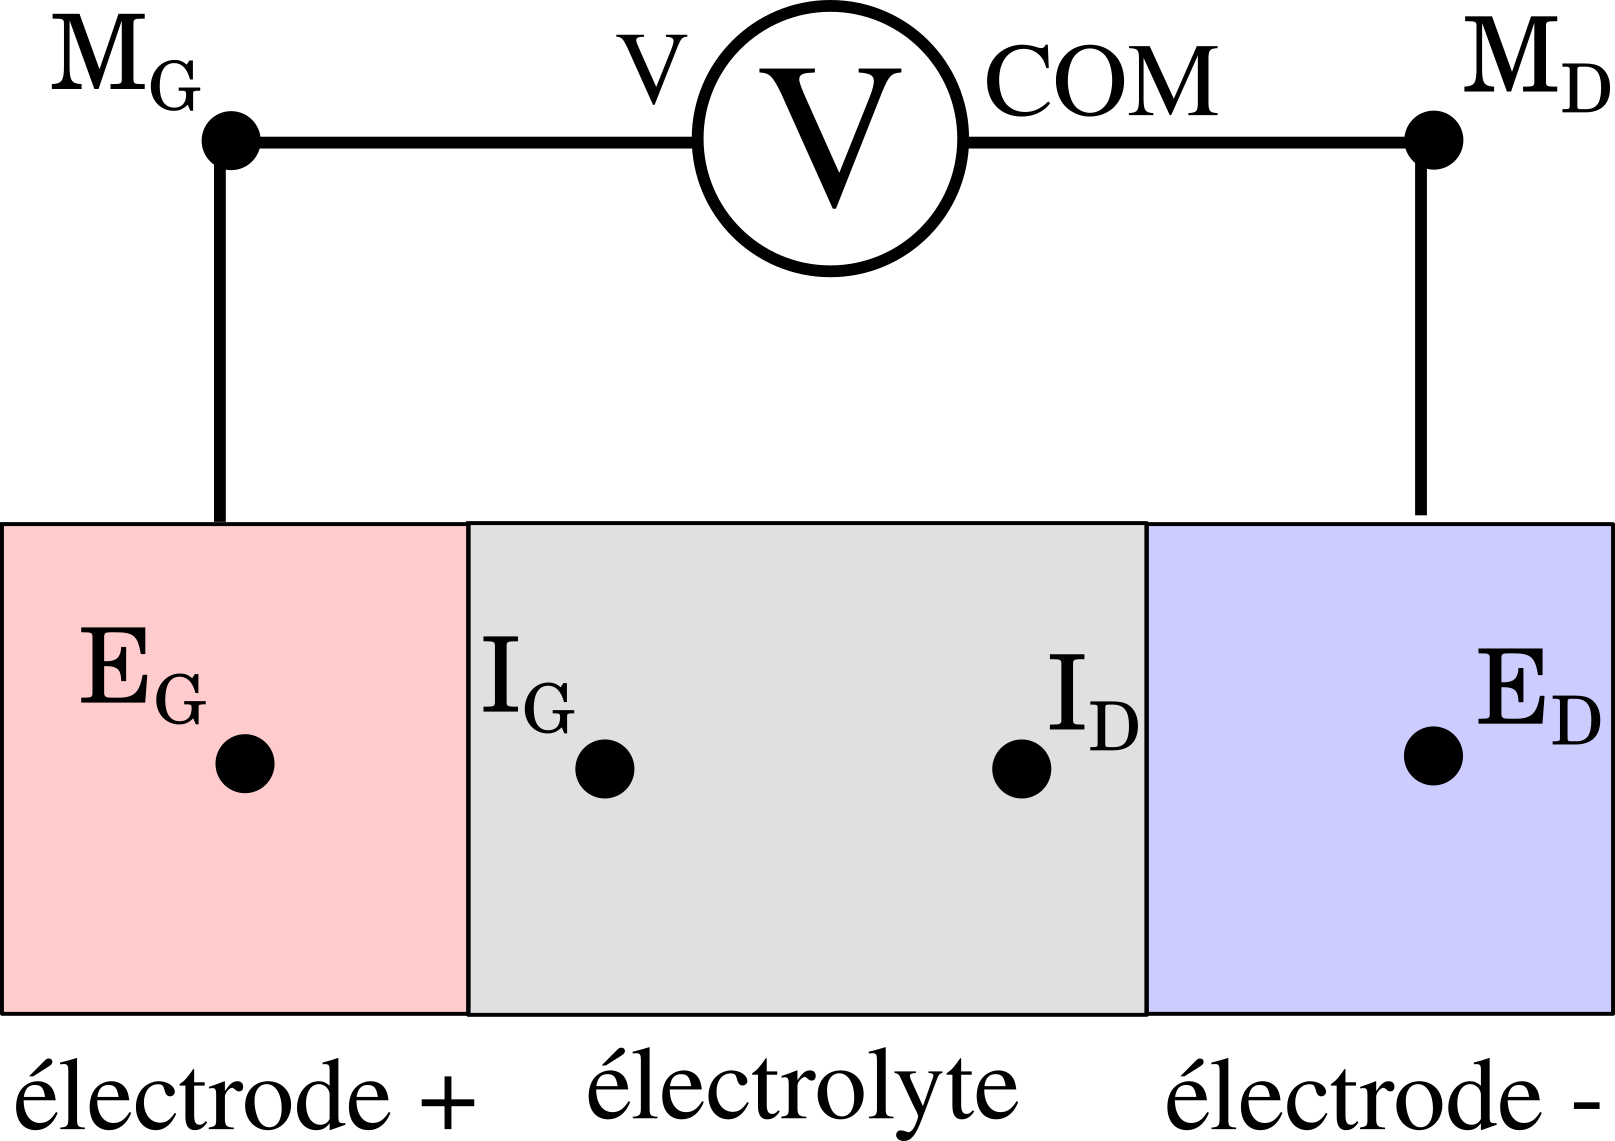
\includegraphics[width=5cm]{figures-Chp0/Fig06}
\captionof{figure}{Représentation des phases mises en jeux au sein d'une batterie (l'électrolyte suppose l'existence éventuelle d'une phase électrolytique en contact avec l'interface, ainsi que d'un éventuel pont salin).}
\end{center}

\begin{align*}
U( I=0 ~ \si{\ampere} ) &= \Phi (M_G) - \Phi (M_D) \\
&= \underbrace{\left ( \Phi (M_G) - \Phi (E_G) \right )}_{K} + \underbrace{\left ( \Phi (E_G) - \Phi (I_G) \right )}_{E_\oplus} \\
& + \underbrace{\left ( \Phi (I_G) - \Phi (I_D) \right )}_{E_j} - \underbrace{\left ( \Phi (E_D) - \Phi (I_D) \right )}_{E_\ominus} \\
& - \underbrace{\left ( \Phi (M_D) - \Phi (E_D) \right )}_{K}
\end{align*}

On remarque cinq termes :
\begin{enumerate}
\item deux potentiels d'interface entre les fils de cuivre et les électrodes, noté $K$. En général, il s'agit un terme constant qui disparaît lorsque l'on étudie des différences de potentiel (ce que l'on fait toujours) ;
\item le potentiel d'électrode au pôle $\oplus$, noté $E_\oplus$ ; 
\item le potentiel de jonction, noté $E_j$ ; 
\item le potentiel d'électrode au pôle $\ominus$, noté $E_\ominus$.
\end{enumerate}

En général, expérimentalement, le potentiel de jonction est négligeable devant la différence des potentiels d'électrode, ce qui nous laisse : 

\begin{align}
U ( I=0 ~ \si{\ampere} ) &= E_\oplus - E_\ominus + E_j  \\
& \approx E_\oplus - E_\ominus
\end{align}}

La tension à courant nul est donc pas définition lié à une différence de potentiel électrique entre l'électrode $\oplus$ et l'électrode $\ominus$. Cette différence de potentiel sous entend l'existence éventuelle d'un champ électrique au sein de la pile, que l'on appelle la force électromotrice de la réaction.

\attention{Dans le restant du cours, nous ferons l'amalgame couramment fait par les chimistes : assimiler la force électromotrice, siglé f.e.m et notée $e$ à la tension à vide $U(I=0 ~ \si{\ampere})$}

\section{Type de réactions}

On va chercher à classer les réactions des cellules électrochimiques utilisant du lithium en deux grandes catégories : 
\begin{enumerate}
\item les cellules qui conduisent à l'apparition et la disparition d'une phase contenant des ions lithiums ;
\item les cellules dans lesquelles les matériaux sont des "éponges" d'ions lithium et sont capables de les accueillir sans qu'il y ait apparition/disparition d'une phase.
\end{enumerate}

Par exemple, un des première batterie brevetée en 1977 par S. Whittimgham utilisait un pôle $\ominus$ en lithium métallique et un pôle $\oplus$ en \ce{TiS2} : 
\begin{center}
\begin{minipage}{0.58\textwidth}
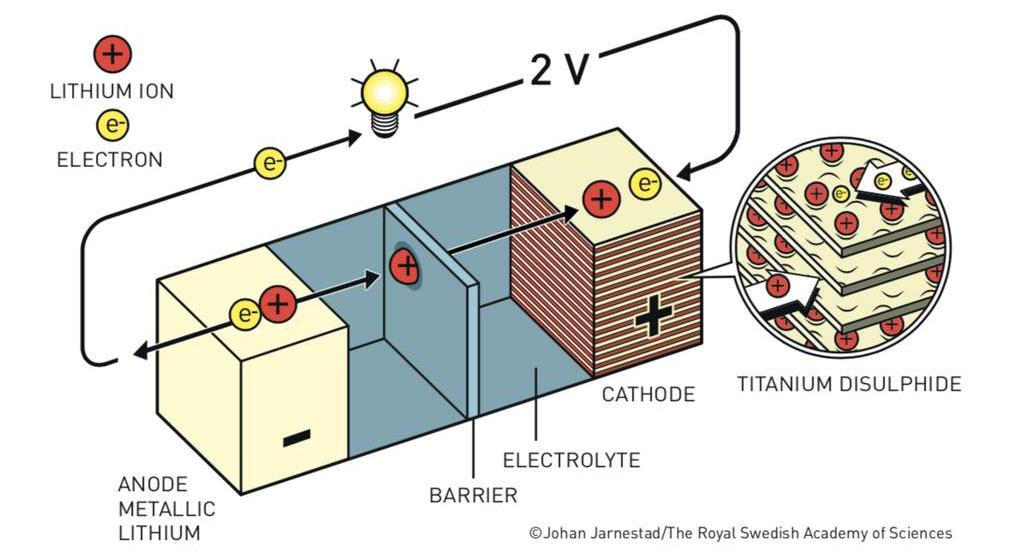
\includegraphics[width=\textwidth]{figures-Chp0/Fig18}
\end{minipage}\hfill\begin{minipage}{0.38\textwidth}
\captionof{figure}{Cellule électrochimique de S. Whittimgham.}
\end{minipage}\end{center}
On voit que \ce{TiS2} est un matériau fonctionnant comme une "éponge" à ions lithium.

\subsection{Réactions de recomposition}

Dans de nombreuses réactions électrochimiques, on observe l'apparition ou la disparition de phases. Par conséquent, cela traduit d'importantes modifications des matériaux d'électrodes, appelé \blancbis{recomposition}.

\subsubsection{dites de formation}

\definition{Une réaction de \blancbis{formation} est une réaction de \blancbis{recomposition} où deux phases réagissent ensemble pour conduire à la formation d'une \blancbis{troisième}. Elles sont modélisées par une équation de réaction de la forme : 
\begin{center}
A + B = AB
\end{center}
La phase AB est formée à partir des composants atomiques des phases A et B.}
%2 Li + Sb = Li2Sb


\subsubsection{dites de déplacement}

\definition{Une réaction de déplacement est une réaction de \blancbis{recomposition} dans laquelle une phase(s) (ou plusieurs) disparaî(ssen)t au profit d'une (de plusieurs) nouvelle(s) phase(s). Elles sont modélisées par une équation de réaction de la forme : 
\begin{center}
A + BX = AX + B
\end{center}
}%2 Li + Cu2O = Li2O + 2Cu

%%EXERCICE

\subsection{Réactions d'insertion}

Il existe une autre catégorie de réaction dans les systèmes électrochimiques où une espèce chimique rédox, accueillie au sein d'un matériau hôte stable migre, lors de la décharge, vers les sites interstitiels inoccupés d'un autre matériau stable.

%Image des deux cas de figure

En général, l'incorporation de l'espèce accueillie à lieu de manière topotactique\mySideNote{\'{E}spèces accueillies s'établissent dans des sites spécifiques de la structure cristalline.} et non pas de manière atactique\mySideNote{\'{E}spèces accueillies s'établissent dans des sites aléatoires de la structure cristalline.}.

\definition{Une réaction d'\blancbis{insertion} est une réaction où une \blancbis{solution solide disparaît} au profit de la \blancbis{formation} d'une nouvelle solution solide.

Elles sont modélisées par une équation de réaction de la forme : 
\begin{align*}
\ce{x A + BX = A_x BX}
\end{align*}
où \ce{A} désigne l'espèce accueillie et \ce{BX} désigne l'espèce hôte.

}
%WARNING Lix + TiS2 = Lix TiS2
Notons dès à présent que dans le cas des matériaux lamellaires\mySideNote{Voir Chp. 3}, les \blancbis{réactions d'insertion} sont parfois appelées \blancbis{réactions d'intercalation}.

\attention{Il est parfois possible qu'une réaction de déplacement se produise par remplacement d'une espèce interstitielle par une autre à l'intérieur d'un matériau hôte. Dans ce cas, une seule phase supplémentaire est formée et on parle d'\blancbis{extrusion} pour décrire ce processus.}
%HCl + LiMO2 = HMO2 + LiCl


\section{Caractériser un accumulateur ou une batterie}

\subsection{Charge, \'{E}nergie \& Puissance}
\subsubsection{Définition}
Les cellules électrochimiques sont des dispositifs électriques. Par conséquent, trois grandeurs électriques usuelles permettent de les caractériser : la charge (notée \textbf{q}), la tension (notée \textbf{U}) et le courant (notée \textbf{I}). Le courant dérive de la charge\mySideNote{Il faut savoir que :
\begin{align*}
I = \frac{dq}{dt}
\end{align*}
}.

Deux grandeurs dérivées des trois grandeurs fondamentales de l'électricité peuvent nous intéresser :

\begin{enumerate}
    \item la puissance électrique instantanée, notée $P$
    \begin{equation}
        P(t) = U(t) I(t)
        \label{eq:puissance}
    \end{equation}
    \item le travail électrique, noté $W'$
    \begin{equation}
        W' = \int_0^t P(t') dt' = \int_0^t U(t') I(t') dt'
        \label{eq:travail}
    \end{equation}
\end{enumerate}

Lorsque le dispositif électrique est en convention récepteur (resp. générateur), la relation Eq. \ref{eq:puissance} nous donne la puissance \blancbis{reçue} (resp. \blancbis{émie}) par le dispositif. De même pour la relation sur le travail Eq. \ref{eq:travail}.

\subsubsection{État de charge}
Afin de caractériser l'état d'une pile ou batterie, on peut utiliser diverses grandeurs dérivées de la capacité permettant de définir son état à un instant $t$.

\definition{
\blancbis{\'{E}tat de charge (SoC, State-of-Charge)} indique la quantité d'énergie emmagasinée par la cellule ou batterie. On la définit comme : 
\begin{equation*}
    SoC [\si{\percent}]= \frac{\text{charge emmagasinée par la batterie}}{\text{charge maximale que peut emmagasiner la batterie}} * 100
    \label{eq:SoC}
\end{equation*}}

Si $SoC =$ \SI{0}{\percent} (resp. \SI{100}{\percent}), la batterie est déchargée (resp. chargée)

\definition{
\blancbis{\'{E}tat de décharge (DoD, Depth-of-Discharged)} indique la quantité d'énergie non emmagasinée par la cellule ou batterie. On la définit comme : 
\begin{equation*}
    DoD [\si{\percent}]= \frac{\text{charge non emmagasinée par la batterie}}{\text{charge maximale que peut emmagasiner la batterie}} * 100
    \label{eq:DoD}
\end{equation*}}

Par définition, $DoD [\si{\percent}] = 100 - SoC [\si{\percent}]$. Si $DoD =$ \SI{0}{\percent} (resp. \SI{100}{\percent}), la batterie est chargée (resp. déchargée)

\subsection{Capacité spécifique (CS)}
\subsubsection{Définition}
La \blancbis{capacité d'une batterie} est définie comme la quantité maximale de charges qui peut être stockée dans la cellule ou batterie. Cette grandeur est \blancbis{extensive}, c'est-à-dire qu'elle dépend de la quantité de matériau présent.\mySideNote{Par opposition, la tension est intensive, elle ne dépend pas de la quantité de matériau présent.}

En général, les chimistes lui préfèrent la \blancbis{capacité spécifique}.

\definition{
La capacité spécifique, notée $CS$, est définie comme : 
\begin{itemize}
\item le rapport de la capacité sur la masse du dispositif, d'où l'appelation de capacité spécifique \blancbis{massique} : 
\begin{align*}
CS_m = \frac{\text{Charge maximale stockable}}{\text{Masse du dispositif}}
\end{align*}
\item le rapport de la capacité sur le volume du dispositif, d'où l'appelation de capacité spécifique \blancbis{volumique} :
\begin{align*}
CS_v = \frac{\text{Charge maximale stockable}}{\text{Volume du dispositif}}
\end{align*}
\end{itemize}

La capacité spécifique s'exprimera en \si{\coulomb\per\kilo\gram} ou \si{\coulomb\per\meter\cubed}
}

L'unité commerciale utilisée est le \si{\ampere\hour\per\kilo\gram}.

%WARNING def
\attention{La capacité \blancbis{spécifique} sera liée à la nature du matériau d'électrode.}

\subsubsection{\'{E}tat de santé (SoH, State-of-Health)} 

\definition{
L'état de santé (SoH, State-of-Health) indique la charge maximale réelle par rapport à la charge maximale théorique que peut contenir la cellule ou la batterie.
\begin{equation*}
    SoH [\si{\percent}]= \frac{\text{capacité maximale réelle}}{\text{capacité maximale théorique}} \times 100
    \label{eq:SoH}
\end{equation*}}

L'état de santé permet de caractériser l'état de vieillissement de votre pile. Si la pile est neuve (resp. usagée), alors $SoH =$ \SI{100}{\percent} (resp. $SoH \to$ \SI{0}{\percent}).

\subsection{Qualité de l'énergie stockée}

La puissance électrique, ainsi que l'énergie, sont liées à la tension à circuit ouvert et par extension à la f.e.m.\mySideNote{La force électromotrice pour ceux qui n'aurait pas suivi =P.}. Nous allons voir au chapitre suivant que la f.e.m. est directement liée à la thermodynamique de la réaction chimique "fictive" ayant lieu entre les espèces chimiques des deux compartiments. Elle est la force motrice permettant la circulation des électrons et le transport des ions à travers l'électrolyte.

En général, du point de vu électrique, la \blancbis{qualité de l'énergie électrique} est supérieure lorsque la tension électrique est élevée. Ceci est simple à comprendre, si vous alimentez une résistance $R$ avec votre pile de f.e.m $e$, la puissance reçue par la résistance est : 
\begin{equation}
P = U_R \cdot I = \frac{e^2}{R}
\end{equation} 

ainsi, du fait du terme en $e^2$; la puissance électrique reçu par un tel dispositif est très sensible à la tension. On peut arbitrairement donner quelques plages de tension, associées aux applications courantes, permettant de définir la qualité de la tension électrique : 
\begin{center}

\begin{tabular}{cc}
$3.5 - 5.5$ \si{\volt} & Grande qualité \\
$1.5 - 3.5$ \si{\volt} & Qualité moyenne \\
$0.0 - 1.5$ \si{\volt} & Qualité faible
\end{tabular}
\end{center}

Cependant, il peut exister des applications allant au délà de ces plages (\emph{par ex.} les voitures électriques nécessitent des tensions autour de \SI{200}{\volt})\mySideNote{Un chimiste ne cherchera pas forcément à optimiser la tension de sortie d'une cellule. En effet, pour certaines applications, comme les semi-conducteurs pour l'électronique, on cherchera en général à avoir de petites tensions (< \SI{1}{\volt}).}.

\subsection{\'{E}nergie théorique maximale (ETM)}
L'énergie théorique maximale est une grandeur permettant de prendre à compte la force électromotrice de la cellule ou batterie et la capacité spécifique et représente l'énergie électrique maximale pouvant être extraite, en théorie, d'une batterie.

\definition{
L'énergie théorique maximale, notée ETM, se définit comme le travail électrique : 
\begin{equation}
ETM = \text{force électromotrice} \times \text{capacité spécifique}
\end{equation}

Elle est en général exprimée en \si{\joule\per\kilo\gram}.}

L'unité commerciale utilisée est le \si{\watt\hour\per\kilo\gram}.

\subsection{Cyclabilité}
Lorsque l'on cherche à réaliser des dispositifs rechargeables, il est fondamental d'étudier \blancbis{la cyclabilité} des dispositifs, c'est-à-dire le nombre de cycle de charge/décharge qu'est capable de faire une batterie avant de perdre complètement sa capacité de charge.

Un dispositif peut être considéré comme toujours fonctionnel si ses caractéristiques électriques : capacité, force électromotrice, énergie stockée$\ldots$ ne sont pas dégradés malgré le cyclage.

On remarque à la Fig. \ref{fig:Chp-0-07}, que pour une perte de la capacité électrique de \SI{0.5}{\percent} à chaque cycle, valeur qui peut sembler anodine, une batterie perd \SI{40}{\percent} de ses capacités en 100 cycles\mySideNote{Tout le travail du chimiste, donc le votre, va être de parvenir à synthétiser des matériaux qui prémunissent de cette diminution de performance.}.

\begin{minipage}{0.65\textwidth}
%% Creator: Matplotlib, PGF backend
%%
%% To include the figure in your LaTeX document, write
%%   \input{<filename>.pgf}
%%
%% Make sure the required packages are loaded in your preamble
%%   \usepackage{pgf}
%%
%% Figures using additional raster images can only be included by \input if
%% they are in the same directory as the main LaTeX file. For loading figures
%% from other directories you can use the `import` package
%%   \usepackage{import}
%% and then include the figures with
%%   \import{<path to file>}{<filename>.pgf}
%%
%% Matplotlib used the following preamble
%%   \usepackage{fontspec}
%%   \setmainfont{DejaVuSerif.ttf}[Path=/home/jeff/anaconda3/envs/h5py/lib/python3.6/site-packages/matplotlib/mpl-data/fonts/ttf/]
%%   \setsansfont{DejaVuSans.ttf}[Path=/home/jeff/anaconda3/envs/h5py/lib/python3.6/site-packages/matplotlib/mpl-data/fonts/ttf/]
%%   \setmonofont{DejaVuSansMono.ttf}[Path=/home/jeff/anaconda3/envs/h5py/lib/python3.6/site-packages/matplotlib/mpl-data/fonts/ttf/]
%%
\begingroup%
\makeatletter%
\begin{pgfpicture}%
\pgfpathrectangle{\pgfpointorigin}{\pgfqpoint{4.000000in}{4.000000in}}%
\pgfusepath{use as bounding box, clip}%
\begin{pgfscope}%
\pgfsetbuttcap%
\pgfsetmiterjoin%
\definecolor{currentfill}{rgb}{1.000000,1.000000,1.000000}%
\pgfsetfillcolor{currentfill}%
\pgfsetlinewidth{0.000000pt}%
\definecolor{currentstroke}{rgb}{1.000000,1.000000,1.000000}%
\pgfsetstrokecolor{currentstroke}%
\pgfsetdash{}{0pt}%
\pgfpathmoveto{\pgfqpoint{0.000000in}{0.000000in}}%
\pgfpathlineto{\pgfqpoint{4.000000in}{0.000000in}}%
\pgfpathlineto{\pgfqpoint{4.000000in}{4.000000in}}%
\pgfpathlineto{\pgfqpoint{0.000000in}{4.000000in}}%
\pgfpathclose%
\pgfusepath{fill}%
\end{pgfscope}%
\begin{pgfscope}%
\pgfsetbuttcap%
\pgfsetmiterjoin%
\definecolor{currentfill}{rgb}{1.000000,1.000000,1.000000}%
\pgfsetfillcolor{currentfill}%
\pgfsetlinewidth{0.000000pt}%
\definecolor{currentstroke}{rgb}{0.000000,0.000000,0.000000}%
\pgfsetstrokecolor{currentstroke}%
\pgfsetstrokeopacity{0.000000}%
\pgfsetdash{}{0pt}%
\pgfpathmoveto{\pgfqpoint{0.500000in}{0.500000in}}%
\pgfpathlineto{\pgfqpoint{2.980000in}{0.500000in}}%
\pgfpathlineto{\pgfqpoint{2.980000in}{3.520000in}}%
\pgfpathlineto{\pgfqpoint{0.500000in}{3.520000in}}%
\pgfpathclose%
\pgfusepath{fill}%
\end{pgfscope}%
\begin{pgfscope}%
\pgfsetbuttcap%
\pgfsetroundjoin%
\definecolor{currentfill}{rgb}{0.000000,0.000000,0.000000}%
\pgfsetfillcolor{currentfill}%
\pgfsetlinewidth{0.803000pt}%
\definecolor{currentstroke}{rgb}{0.000000,0.000000,0.000000}%
\pgfsetstrokecolor{currentstroke}%
\pgfsetdash{}{0pt}%
\pgfsys@defobject{currentmarker}{\pgfqpoint{0.000000in}{-0.048611in}}{\pgfqpoint{0.000000in}{0.000000in}}{%
\pgfpathmoveto{\pgfqpoint{0.000000in}{0.000000in}}%
\pgfpathlineto{\pgfqpoint{0.000000in}{-0.048611in}}%
\pgfusepath{stroke,fill}%
}%
\begin{pgfscope}%
\pgfsys@transformshift{0.500000in}{0.500000in}%
\pgfsys@useobject{currentmarker}{}%
\end{pgfscope}%
\end{pgfscope}%
\begin{pgfscope}%
\definecolor{textcolor}{rgb}{0.000000,0.000000,0.000000}%
\pgfsetstrokecolor{textcolor}%
\pgfsetfillcolor{textcolor}%
\pgftext[x=0.500000in,y=0.402778in,,top]{\color{textcolor}\rmfamily\fontsize{10.000000}{12.000000}\selectfont \(\displaystyle 0\)}%
\end{pgfscope}%
\begin{pgfscope}%
\pgfsetbuttcap%
\pgfsetroundjoin%
\definecolor{currentfill}{rgb}{0.000000,0.000000,0.000000}%
\pgfsetfillcolor{currentfill}%
\pgfsetlinewidth{0.803000pt}%
\definecolor{currentstroke}{rgb}{0.000000,0.000000,0.000000}%
\pgfsetstrokecolor{currentstroke}%
\pgfsetdash{}{0pt}%
\pgfsys@defobject{currentmarker}{\pgfqpoint{0.000000in}{-0.048611in}}{\pgfqpoint{0.000000in}{0.000000in}}{%
\pgfpathmoveto{\pgfqpoint{0.000000in}{0.000000in}}%
\pgfpathlineto{\pgfqpoint{0.000000in}{-0.048611in}}%
\pgfusepath{stroke,fill}%
}%
\begin{pgfscope}%
\pgfsys@transformshift{1.090476in}{0.500000in}%
\pgfsys@useobject{currentmarker}{}%
\end{pgfscope}%
\end{pgfscope}%
\begin{pgfscope}%
\definecolor{textcolor}{rgb}{0.000000,0.000000,0.000000}%
\pgfsetstrokecolor{textcolor}%
\pgfsetfillcolor{textcolor}%
\pgftext[x=1.090476in,y=0.402778in,,top]{\color{textcolor}\rmfamily\fontsize{10.000000}{12.000000}\selectfont \(\displaystyle 25\)}%
\end{pgfscope}%
\begin{pgfscope}%
\pgfsetbuttcap%
\pgfsetroundjoin%
\definecolor{currentfill}{rgb}{0.000000,0.000000,0.000000}%
\pgfsetfillcolor{currentfill}%
\pgfsetlinewidth{0.803000pt}%
\definecolor{currentstroke}{rgb}{0.000000,0.000000,0.000000}%
\pgfsetstrokecolor{currentstroke}%
\pgfsetdash{}{0pt}%
\pgfsys@defobject{currentmarker}{\pgfqpoint{0.000000in}{-0.048611in}}{\pgfqpoint{0.000000in}{0.000000in}}{%
\pgfpathmoveto{\pgfqpoint{0.000000in}{0.000000in}}%
\pgfpathlineto{\pgfqpoint{0.000000in}{-0.048611in}}%
\pgfusepath{stroke,fill}%
}%
\begin{pgfscope}%
\pgfsys@transformshift{1.680952in}{0.500000in}%
\pgfsys@useobject{currentmarker}{}%
\end{pgfscope}%
\end{pgfscope}%
\begin{pgfscope}%
\definecolor{textcolor}{rgb}{0.000000,0.000000,0.000000}%
\pgfsetstrokecolor{textcolor}%
\pgfsetfillcolor{textcolor}%
\pgftext[x=1.680952in,y=0.402778in,,top]{\color{textcolor}\rmfamily\fontsize{10.000000}{12.000000}\selectfont \(\displaystyle 50\)}%
\end{pgfscope}%
\begin{pgfscope}%
\pgfsetbuttcap%
\pgfsetroundjoin%
\definecolor{currentfill}{rgb}{0.000000,0.000000,0.000000}%
\pgfsetfillcolor{currentfill}%
\pgfsetlinewidth{0.803000pt}%
\definecolor{currentstroke}{rgb}{0.000000,0.000000,0.000000}%
\pgfsetstrokecolor{currentstroke}%
\pgfsetdash{}{0pt}%
\pgfsys@defobject{currentmarker}{\pgfqpoint{0.000000in}{-0.048611in}}{\pgfqpoint{0.000000in}{0.000000in}}{%
\pgfpathmoveto{\pgfqpoint{0.000000in}{0.000000in}}%
\pgfpathlineto{\pgfqpoint{0.000000in}{-0.048611in}}%
\pgfusepath{stroke,fill}%
}%
\begin{pgfscope}%
\pgfsys@transformshift{2.271429in}{0.500000in}%
\pgfsys@useobject{currentmarker}{}%
\end{pgfscope}%
\end{pgfscope}%
\begin{pgfscope}%
\definecolor{textcolor}{rgb}{0.000000,0.000000,0.000000}%
\pgfsetstrokecolor{textcolor}%
\pgfsetfillcolor{textcolor}%
\pgftext[x=2.271429in,y=0.402778in,,top]{\color{textcolor}\rmfamily\fontsize{10.000000}{12.000000}\selectfont \(\displaystyle 75\)}%
\end{pgfscope}%
\begin{pgfscope}%
\pgfsetbuttcap%
\pgfsetroundjoin%
\definecolor{currentfill}{rgb}{0.000000,0.000000,0.000000}%
\pgfsetfillcolor{currentfill}%
\pgfsetlinewidth{0.803000pt}%
\definecolor{currentstroke}{rgb}{0.000000,0.000000,0.000000}%
\pgfsetstrokecolor{currentstroke}%
\pgfsetdash{}{0pt}%
\pgfsys@defobject{currentmarker}{\pgfqpoint{0.000000in}{-0.048611in}}{\pgfqpoint{0.000000in}{0.000000in}}{%
\pgfpathmoveto{\pgfqpoint{0.000000in}{0.000000in}}%
\pgfpathlineto{\pgfqpoint{0.000000in}{-0.048611in}}%
\pgfusepath{stroke,fill}%
}%
\begin{pgfscope}%
\pgfsys@transformshift{2.861905in}{0.500000in}%
\pgfsys@useobject{currentmarker}{}%
\end{pgfscope}%
\end{pgfscope}%
\begin{pgfscope}%
\definecolor{textcolor}{rgb}{0.000000,0.000000,0.000000}%
\pgfsetstrokecolor{textcolor}%
\pgfsetfillcolor{textcolor}%
\pgftext[x=2.861905in,y=0.402778in,,top]{\color{textcolor}\rmfamily\fontsize{10.000000}{12.000000}\selectfont \(\displaystyle 100\)}%
\end{pgfscope}%
\begin{pgfscope}%
\definecolor{textcolor}{rgb}{0.000000,0.000000,0.000000}%
\pgfsetstrokecolor{textcolor}%
\pgfsetfillcolor{textcolor}%
\pgftext[x=1.740000in,y=0.212809in,,top]{\color{textcolor}\rmfamily\fontsize{10.000000}{12.000000}\selectfont Nombre de cycles de charge/décharge}%
\end{pgfscope}%
\begin{pgfscope}%
\pgfsetbuttcap%
\pgfsetroundjoin%
\definecolor{currentfill}{rgb}{0.000000,0.000000,0.000000}%
\pgfsetfillcolor{currentfill}%
\pgfsetlinewidth{0.803000pt}%
\definecolor{currentstroke}{rgb}{0.000000,0.000000,0.000000}%
\pgfsetstrokecolor{currentstroke}%
\pgfsetdash{}{0pt}%
\pgfsys@defobject{currentmarker}{\pgfqpoint{-0.048611in}{0.000000in}}{\pgfqpoint{0.000000in}{0.000000in}}{%
\pgfpathmoveto{\pgfqpoint{0.000000in}{0.000000in}}%
\pgfpathlineto{\pgfqpoint{-0.048611in}{0.000000in}}%
\pgfusepath{stroke,fill}%
}%
\begin{pgfscope}%
\pgfsys@transformshift{0.500000in}{0.500000in}%
\pgfsys@useobject{currentmarker}{}%
\end{pgfscope}%
\end{pgfscope}%
\begin{pgfscope}%
\definecolor{textcolor}{rgb}{0.000000,0.000000,0.000000}%
\pgfsetstrokecolor{textcolor}%
\pgfsetfillcolor{textcolor}%
\pgftext[x=0.333333in,y=0.447238in,left,base]{\color{textcolor}\rmfamily\fontsize{10.000000}{12.000000}\selectfont \(\displaystyle 0\)}%
\end{pgfscope}%
\begin{pgfscope}%
\pgfsetbuttcap%
\pgfsetroundjoin%
\definecolor{currentfill}{rgb}{0.000000,0.000000,0.000000}%
\pgfsetfillcolor{currentfill}%
\pgfsetlinewidth{0.803000pt}%
\definecolor{currentstroke}{rgb}{0.000000,0.000000,0.000000}%
\pgfsetstrokecolor{currentstroke}%
\pgfsetdash{}{0pt}%
\pgfsys@defobject{currentmarker}{\pgfqpoint{-0.048611in}{0.000000in}}{\pgfqpoint{0.000000in}{0.000000in}}{%
\pgfpathmoveto{\pgfqpoint{0.000000in}{0.000000in}}%
\pgfpathlineto{\pgfqpoint{-0.048611in}{0.000000in}}%
\pgfusepath{stroke,fill}%
}%
\begin{pgfscope}%
\pgfsys@transformshift{0.500000in}{1.075400in}%
\pgfsys@useobject{currentmarker}{}%
\end{pgfscope}%
\end{pgfscope}%
\begin{pgfscope}%
\definecolor{textcolor}{rgb}{0.000000,0.000000,0.000000}%
\pgfsetstrokecolor{textcolor}%
\pgfsetfillcolor{textcolor}%
\pgftext[x=0.263888in,y=1.022639in,left,base]{\color{textcolor}\rmfamily\fontsize{10.000000}{12.000000}\selectfont \(\displaystyle 20\)}%
\end{pgfscope}%
\begin{pgfscope}%
\pgfsetbuttcap%
\pgfsetroundjoin%
\definecolor{currentfill}{rgb}{0.000000,0.000000,0.000000}%
\pgfsetfillcolor{currentfill}%
\pgfsetlinewidth{0.803000pt}%
\definecolor{currentstroke}{rgb}{0.000000,0.000000,0.000000}%
\pgfsetstrokecolor{currentstroke}%
\pgfsetdash{}{0pt}%
\pgfsys@defobject{currentmarker}{\pgfqpoint{-0.048611in}{0.000000in}}{\pgfqpoint{0.000000in}{0.000000in}}{%
\pgfpathmoveto{\pgfqpoint{0.000000in}{0.000000in}}%
\pgfpathlineto{\pgfqpoint{-0.048611in}{0.000000in}}%
\pgfusepath{stroke,fill}%
}%
\begin{pgfscope}%
\pgfsys@transformshift{0.500000in}{1.650801in}%
\pgfsys@useobject{currentmarker}{}%
\end{pgfscope}%
\end{pgfscope}%
\begin{pgfscope}%
\definecolor{textcolor}{rgb}{0.000000,0.000000,0.000000}%
\pgfsetstrokecolor{textcolor}%
\pgfsetfillcolor{textcolor}%
\pgftext[x=0.263888in,y=1.598039in,left,base]{\color{textcolor}\rmfamily\fontsize{10.000000}{12.000000}\selectfont \(\displaystyle 40\)}%
\end{pgfscope}%
\begin{pgfscope}%
\pgfsetbuttcap%
\pgfsetroundjoin%
\definecolor{currentfill}{rgb}{0.000000,0.000000,0.000000}%
\pgfsetfillcolor{currentfill}%
\pgfsetlinewidth{0.803000pt}%
\definecolor{currentstroke}{rgb}{0.000000,0.000000,0.000000}%
\pgfsetstrokecolor{currentstroke}%
\pgfsetdash{}{0pt}%
\pgfsys@defobject{currentmarker}{\pgfqpoint{-0.048611in}{0.000000in}}{\pgfqpoint{0.000000in}{0.000000in}}{%
\pgfpathmoveto{\pgfqpoint{0.000000in}{0.000000in}}%
\pgfpathlineto{\pgfqpoint{-0.048611in}{0.000000in}}%
\pgfusepath{stroke,fill}%
}%
\begin{pgfscope}%
\pgfsys@transformshift{0.500000in}{2.226201in}%
\pgfsys@useobject{currentmarker}{}%
\end{pgfscope}%
\end{pgfscope}%
\begin{pgfscope}%
\definecolor{textcolor}{rgb}{0.000000,0.000000,0.000000}%
\pgfsetstrokecolor{textcolor}%
\pgfsetfillcolor{textcolor}%
\pgftext[x=0.263888in,y=2.173439in,left,base]{\color{textcolor}\rmfamily\fontsize{10.000000}{12.000000}\selectfont \(\displaystyle 60\)}%
\end{pgfscope}%
\begin{pgfscope}%
\pgfsetbuttcap%
\pgfsetroundjoin%
\definecolor{currentfill}{rgb}{0.000000,0.000000,0.000000}%
\pgfsetfillcolor{currentfill}%
\pgfsetlinewidth{0.803000pt}%
\definecolor{currentstroke}{rgb}{0.000000,0.000000,0.000000}%
\pgfsetstrokecolor{currentstroke}%
\pgfsetdash{}{0pt}%
\pgfsys@defobject{currentmarker}{\pgfqpoint{-0.048611in}{0.000000in}}{\pgfqpoint{0.000000in}{0.000000in}}{%
\pgfpathmoveto{\pgfqpoint{0.000000in}{0.000000in}}%
\pgfpathlineto{\pgfqpoint{-0.048611in}{0.000000in}}%
\pgfusepath{stroke,fill}%
}%
\begin{pgfscope}%
\pgfsys@transformshift{0.500000in}{2.801601in}%
\pgfsys@useobject{currentmarker}{}%
\end{pgfscope}%
\end{pgfscope}%
\begin{pgfscope}%
\definecolor{textcolor}{rgb}{0.000000,0.000000,0.000000}%
\pgfsetstrokecolor{textcolor}%
\pgfsetfillcolor{textcolor}%
\pgftext[x=0.263888in,y=2.748840in,left,base]{\color{textcolor}\rmfamily\fontsize{10.000000}{12.000000}\selectfont \(\displaystyle 80\)}%
\end{pgfscope}%
\begin{pgfscope}%
\pgfsetbuttcap%
\pgfsetroundjoin%
\definecolor{currentfill}{rgb}{0.000000,0.000000,0.000000}%
\pgfsetfillcolor{currentfill}%
\pgfsetlinewidth{0.803000pt}%
\definecolor{currentstroke}{rgb}{0.000000,0.000000,0.000000}%
\pgfsetstrokecolor{currentstroke}%
\pgfsetdash{}{0pt}%
\pgfsys@defobject{currentmarker}{\pgfqpoint{-0.048611in}{0.000000in}}{\pgfqpoint{0.000000in}{0.000000in}}{%
\pgfpathmoveto{\pgfqpoint{0.000000in}{0.000000in}}%
\pgfpathlineto{\pgfqpoint{-0.048611in}{0.000000in}}%
\pgfusepath{stroke,fill}%
}%
\begin{pgfscope}%
\pgfsys@transformshift{0.500000in}{3.377002in}%
\pgfsys@useobject{currentmarker}{}%
\end{pgfscope}%
\end{pgfscope}%
\begin{pgfscope}%
\definecolor{textcolor}{rgb}{0.000000,0.000000,0.000000}%
\pgfsetstrokecolor{textcolor}%
\pgfsetfillcolor{textcolor}%
\pgftext[x=0.194444in,y=3.324240in,left,base]{\color{textcolor}\rmfamily\fontsize{10.000000}{12.000000}\selectfont \(\displaystyle 100\)}%
\end{pgfscope}%
\begin{pgfscope}%
\definecolor{textcolor}{rgb}{0.000000,0.000000,0.000000}%
\pgfsetstrokecolor{textcolor}%
\pgfsetfillcolor{textcolor}%
\pgftext[x=0.138888in,y=2.010000in,,bottom,rotate=90.000000]{\color{textcolor}\rmfamily\fontsize{10.000000}{12.000000}\selectfont Pourcentage de perte de la capacité initiale}%
\end{pgfscope}%
\begin{pgfscope}%
\pgfpathrectangle{\pgfqpoint{0.500000in}{0.500000in}}{\pgfqpoint{2.480000in}{3.020000in}}%
\pgfusepath{clip}%
\pgfsetbuttcap%
\pgfsetroundjoin%
\definecolor{currentfill}{rgb}{0.229806,0.298718,0.753683}%
\pgfsetfillcolor{currentfill}%
\pgfsetlinewidth{1.003750pt}%
\definecolor{currentstroke}{rgb}{0.229806,0.298718,0.753683}%
\pgfsetstrokecolor{currentstroke}%
\pgfsetdash{}{0pt}%
\pgfsys@defobject{currentmarker}{\pgfqpoint{-0.034722in}{-0.034722in}}{\pgfqpoint{0.034722in}{0.034722in}}{%
\pgfpathmoveto{\pgfqpoint{0.000000in}{-0.034722in}}%
\pgfpathcurveto{\pgfqpoint{0.009208in}{-0.034722in}}{\pgfqpoint{0.018041in}{-0.031064in}}{\pgfqpoint{0.024552in}{-0.024552in}}%
\pgfpathcurveto{\pgfqpoint{0.031064in}{-0.018041in}}{\pgfqpoint{0.034722in}{-0.009208in}}{\pgfqpoint{0.034722in}{0.000000in}}%
\pgfpathcurveto{\pgfqpoint{0.034722in}{0.009208in}}{\pgfqpoint{0.031064in}{0.018041in}}{\pgfqpoint{0.024552in}{0.024552in}}%
\pgfpathcurveto{\pgfqpoint{0.018041in}{0.031064in}}{\pgfqpoint{0.009208in}{0.034722in}}{\pgfqpoint{0.000000in}{0.034722in}}%
\pgfpathcurveto{\pgfqpoint{-0.009208in}{0.034722in}}{\pgfqpoint{-0.018041in}{0.031064in}}{\pgfqpoint{-0.024552in}{0.024552in}}%
\pgfpathcurveto{\pgfqpoint{-0.031064in}{0.018041in}}{\pgfqpoint{-0.034722in}{0.009208in}}{\pgfqpoint{-0.034722in}{0.000000in}}%
\pgfpathcurveto{\pgfqpoint{-0.034722in}{-0.009208in}}{\pgfqpoint{-0.031064in}{-0.018041in}}{\pgfqpoint{-0.024552in}{-0.024552in}}%
\pgfpathcurveto{\pgfqpoint{-0.018041in}{-0.031064in}}{\pgfqpoint{-0.009208in}{-0.034722in}}{\pgfqpoint{0.000000in}{-0.034722in}}%
\pgfpathclose%
\pgfusepath{stroke,fill}%
}%
\begin{pgfscope}%
\pgfsys@transformshift{0.500000in}{3.377002in}%
\pgfsys@useobject{currentmarker}{}%
\end{pgfscope}%
\begin{pgfscope}%
\pgfsys@transformshift{0.548202in}{3.377002in}%
\pgfsys@useobject{currentmarker}{}%
\end{pgfscope}%
\begin{pgfscope}%
\pgfsys@transformshift{0.596404in}{3.377002in}%
\pgfsys@useobject{currentmarker}{}%
\end{pgfscope}%
\begin{pgfscope}%
\pgfsys@transformshift{0.644606in}{3.377002in}%
\pgfsys@useobject{currentmarker}{}%
\end{pgfscope}%
\begin{pgfscope}%
\pgfsys@transformshift{0.692809in}{3.377002in}%
\pgfsys@useobject{currentmarker}{}%
\end{pgfscope}%
\begin{pgfscope}%
\pgfsys@transformshift{0.741011in}{3.377002in}%
\pgfsys@useobject{currentmarker}{}%
\end{pgfscope}%
\begin{pgfscope}%
\pgfsys@transformshift{0.789213in}{3.377002in}%
\pgfsys@useobject{currentmarker}{}%
\end{pgfscope}%
\begin{pgfscope}%
\pgfsys@transformshift{0.837415in}{3.377002in}%
\pgfsys@useobject{currentmarker}{}%
\end{pgfscope}%
\begin{pgfscope}%
\pgfsys@transformshift{0.885617in}{3.377002in}%
\pgfsys@useobject{currentmarker}{}%
\end{pgfscope}%
\begin{pgfscope}%
\pgfsys@transformshift{0.933819in}{3.377002in}%
\pgfsys@useobject{currentmarker}{}%
\end{pgfscope}%
\begin{pgfscope}%
\pgfsys@transformshift{0.982021in}{3.377002in}%
\pgfsys@useobject{currentmarker}{}%
\end{pgfscope}%
\begin{pgfscope}%
\pgfsys@transformshift{1.030224in}{3.377002in}%
\pgfsys@useobject{currentmarker}{}%
\end{pgfscope}%
\begin{pgfscope}%
\pgfsys@transformshift{1.078426in}{3.377002in}%
\pgfsys@useobject{currentmarker}{}%
\end{pgfscope}%
\begin{pgfscope}%
\pgfsys@transformshift{1.126628in}{3.377002in}%
\pgfsys@useobject{currentmarker}{}%
\end{pgfscope}%
\begin{pgfscope}%
\pgfsys@transformshift{1.174830in}{3.377002in}%
\pgfsys@useobject{currentmarker}{}%
\end{pgfscope}%
\begin{pgfscope}%
\pgfsys@transformshift{1.223032in}{3.377002in}%
\pgfsys@useobject{currentmarker}{}%
\end{pgfscope}%
\begin{pgfscope}%
\pgfsys@transformshift{1.271234in}{3.377002in}%
\pgfsys@useobject{currentmarker}{}%
\end{pgfscope}%
\begin{pgfscope}%
\pgfsys@transformshift{1.319436in}{3.377002in}%
\pgfsys@useobject{currentmarker}{}%
\end{pgfscope}%
\begin{pgfscope}%
\pgfsys@transformshift{1.367638in}{3.377002in}%
\pgfsys@useobject{currentmarker}{}%
\end{pgfscope}%
\begin{pgfscope}%
\pgfsys@transformshift{1.415841in}{3.377002in}%
\pgfsys@useobject{currentmarker}{}%
\end{pgfscope}%
\begin{pgfscope}%
\pgfsys@transformshift{1.464043in}{3.377002in}%
\pgfsys@useobject{currentmarker}{}%
\end{pgfscope}%
\begin{pgfscope}%
\pgfsys@transformshift{1.512245in}{3.377002in}%
\pgfsys@useobject{currentmarker}{}%
\end{pgfscope}%
\begin{pgfscope}%
\pgfsys@transformshift{1.560447in}{3.377002in}%
\pgfsys@useobject{currentmarker}{}%
\end{pgfscope}%
\begin{pgfscope}%
\pgfsys@transformshift{1.608649in}{3.377002in}%
\pgfsys@useobject{currentmarker}{}%
\end{pgfscope}%
\begin{pgfscope}%
\pgfsys@transformshift{1.656851in}{3.377002in}%
\pgfsys@useobject{currentmarker}{}%
\end{pgfscope}%
\begin{pgfscope}%
\pgfsys@transformshift{1.705053in}{3.377002in}%
\pgfsys@useobject{currentmarker}{}%
\end{pgfscope}%
\begin{pgfscope}%
\pgfsys@transformshift{1.753256in}{3.377002in}%
\pgfsys@useobject{currentmarker}{}%
\end{pgfscope}%
\begin{pgfscope}%
\pgfsys@transformshift{1.801458in}{3.377002in}%
\pgfsys@useobject{currentmarker}{}%
\end{pgfscope}%
\begin{pgfscope}%
\pgfsys@transformshift{1.849660in}{3.377002in}%
\pgfsys@useobject{currentmarker}{}%
\end{pgfscope}%
\begin{pgfscope}%
\pgfsys@transformshift{1.897862in}{3.377002in}%
\pgfsys@useobject{currentmarker}{}%
\end{pgfscope}%
\begin{pgfscope}%
\pgfsys@transformshift{1.946064in}{3.377002in}%
\pgfsys@useobject{currentmarker}{}%
\end{pgfscope}%
\begin{pgfscope}%
\pgfsys@transformshift{1.994266in}{3.377002in}%
\pgfsys@useobject{currentmarker}{}%
\end{pgfscope}%
\begin{pgfscope}%
\pgfsys@transformshift{2.042468in}{3.377002in}%
\pgfsys@useobject{currentmarker}{}%
\end{pgfscope}%
\begin{pgfscope}%
\pgfsys@transformshift{2.090671in}{3.377002in}%
\pgfsys@useobject{currentmarker}{}%
\end{pgfscope}%
\begin{pgfscope}%
\pgfsys@transformshift{2.138873in}{3.377002in}%
\pgfsys@useobject{currentmarker}{}%
\end{pgfscope}%
\begin{pgfscope}%
\pgfsys@transformshift{2.187075in}{3.377002in}%
\pgfsys@useobject{currentmarker}{}%
\end{pgfscope}%
\begin{pgfscope}%
\pgfsys@transformshift{2.235277in}{3.377002in}%
\pgfsys@useobject{currentmarker}{}%
\end{pgfscope}%
\begin{pgfscope}%
\pgfsys@transformshift{2.283479in}{3.377002in}%
\pgfsys@useobject{currentmarker}{}%
\end{pgfscope}%
\begin{pgfscope}%
\pgfsys@transformshift{2.331681in}{3.377002in}%
\pgfsys@useobject{currentmarker}{}%
\end{pgfscope}%
\begin{pgfscope}%
\pgfsys@transformshift{2.379883in}{3.377002in}%
\pgfsys@useobject{currentmarker}{}%
\end{pgfscope}%
\begin{pgfscope}%
\pgfsys@transformshift{2.428086in}{3.377002in}%
\pgfsys@useobject{currentmarker}{}%
\end{pgfscope}%
\begin{pgfscope}%
\pgfsys@transformshift{2.476288in}{3.377002in}%
\pgfsys@useobject{currentmarker}{}%
\end{pgfscope}%
\begin{pgfscope}%
\pgfsys@transformshift{2.524490in}{3.377002in}%
\pgfsys@useobject{currentmarker}{}%
\end{pgfscope}%
\begin{pgfscope}%
\pgfsys@transformshift{2.572692in}{3.377002in}%
\pgfsys@useobject{currentmarker}{}%
\end{pgfscope}%
\begin{pgfscope}%
\pgfsys@transformshift{2.620894in}{3.377002in}%
\pgfsys@useobject{currentmarker}{}%
\end{pgfscope}%
\begin{pgfscope}%
\pgfsys@transformshift{2.669096in}{3.377002in}%
\pgfsys@useobject{currentmarker}{}%
\end{pgfscope}%
\begin{pgfscope}%
\pgfsys@transformshift{2.717298in}{3.377002in}%
\pgfsys@useobject{currentmarker}{}%
\end{pgfscope}%
\begin{pgfscope}%
\pgfsys@transformshift{2.765500in}{3.377002in}%
\pgfsys@useobject{currentmarker}{}%
\end{pgfscope}%
\begin{pgfscope}%
\pgfsys@transformshift{2.813703in}{3.377002in}%
\pgfsys@useobject{currentmarker}{}%
\end{pgfscope}%
\begin{pgfscope}%
\pgfsys@transformshift{2.861905in}{3.377002in}%
\pgfsys@useobject{currentmarker}{}%
\end{pgfscope}%
\end{pgfscope}%
\begin{pgfscope}%
\pgfpathrectangle{\pgfqpoint{0.500000in}{0.500000in}}{\pgfqpoint{2.480000in}{3.020000in}}%
\pgfusepath{clip}%
\pgfsetbuttcap%
\pgfsetroundjoin%
\definecolor{currentfill}{rgb}{0.552953,0.688929,0.995376}%
\pgfsetfillcolor{currentfill}%
\pgfsetlinewidth{1.003750pt}%
\definecolor{currentstroke}{rgb}{0.552953,0.688929,0.995376}%
\pgfsetstrokecolor{currentstroke}%
\pgfsetdash{}{0pt}%
\pgfsys@defobject{currentmarker}{\pgfqpoint{-0.034722in}{-0.034722in}}{\pgfqpoint{0.034722in}{0.034722in}}{%
\pgfpathmoveto{\pgfqpoint{0.000000in}{-0.034722in}}%
\pgfpathcurveto{\pgfqpoint{0.009208in}{-0.034722in}}{\pgfqpoint{0.018041in}{-0.031064in}}{\pgfqpoint{0.024552in}{-0.024552in}}%
\pgfpathcurveto{\pgfqpoint{0.031064in}{-0.018041in}}{\pgfqpoint{0.034722in}{-0.009208in}}{\pgfqpoint{0.034722in}{0.000000in}}%
\pgfpathcurveto{\pgfqpoint{0.034722in}{0.009208in}}{\pgfqpoint{0.031064in}{0.018041in}}{\pgfqpoint{0.024552in}{0.024552in}}%
\pgfpathcurveto{\pgfqpoint{0.018041in}{0.031064in}}{\pgfqpoint{0.009208in}{0.034722in}}{\pgfqpoint{0.000000in}{0.034722in}}%
\pgfpathcurveto{\pgfqpoint{-0.009208in}{0.034722in}}{\pgfqpoint{-0.018041in}{0.031064in}}{\pgfqpoint{-0.024552in}{0.024552in}}%
\pgfpathcurveto{\pgfqpoint{-0.031064in}{0.018041in}}{\pgfqpoint{-0.034722in}{0.009208in}}{\pgfqpoint{-0.034722in}{0.000000in}}%
\pgfpathcurveto{\pgfqpoint{-0.034722in}{-0.009208in}}{\pgfqpoint{-0.031064in}{-0.018041in}}{\pgfqpoint{-0.024552in}{-0.024552in}}%
\pgfpathcurveto{\pgfqpoint{-0.018041in}{-0.031064in}}{\pgfqpoint{-0.009208in}{-0.034722in}}{\pgfqpoint{0.000000in}{-0.034722in}}%
\pgfpathclose%
\pgfusepath{stroke,fill}%
}%
\begin{pgfscope}%
\pgfsys@transformshift{0.500000in}{3.377002in}%
\pgfsys@useobject{currentmarker}{}%
\end{pgfscope}%
\begin{pgfscope}%
\pgfsys@transformshift{0.548202in}{3.347721in}%
\pgfsys@useobject{currentmarker}{}%
\end{pgfscope}%
\begin{pgfscope}%
\pgfsys@transformshift{0.596404in}{3.318738in}%
\pgfsys@useobject{currentmarker}{}%
\end{pgfscope}%
\begin{pgfscope}%
\pgfsys@transformshift{0.644606in}{3.290050in}%
\pgfsys@useobject{currentmarker}{}%
\end{pgfscope}%
\begin{pgfscope}%
\pgfsys@transformshift{0.692809in}{3.261654in}%
\pgfsys@useobject{currentmarker}{}%
\end{pgfscope}%
\begin{pgfscope}%
\pgfsys@transformshift{0.741011in}{3.233548in}%
\pgfsys@useobject{currentmarker}{}%
\end{pgfscope}%
\begin{pgfscope}%
\pgfsys@transformshift{0.789213in}{3.205727in}%
\pgfsys@useobject{currentmarker}{}%
\end{pgfscope}%
\begin{pgfscope}%
\pgfsys@transformshift{0.837415in}{3.178189in}%
\pgfsys@useobject{currentmarker}{}%
\end{pgfscope}%
\begin{pgfscope}%
\pgfsys@transformshift{0.885617in}{3.150932in}%
\pgfsys@useobject{currentmarker}{}%
\end{pgfscope}%
\begin{pgfscope}%
\pgfsys@transformshift{0.933819in}{3.123952in}%
\pgfsys@useobject{currentmarker}{}%
\end{pgfscope}%
\begin{pgfscope}%
\pgfsys@transformshift{0.982021in}{3.097247in}%
\pgfsys@useobject{currentmarker}{}%
\end{pgfscope}%
\begin{pgfscope}%
\pgfsys@transformshift{1.030224in}{3.070813in}%
\pgfsys@useobject{currentmarker}{}%
\end{pgfscope}%
\begin{pgfscope}%
\pgfsys@transformshift{1.078426in}{3.044648in}%
\pgfsys@useobject{currentmarker}{}%
\end{pgfscope}%
\begin{pgfscope}%
\pgfsys@transformshift{1.126628in}{3.018750in}%
\pgfsys@useobject{currentmarker}{}%
\end{pgfscope}%
\begin{pgfscope}%
\pgfsys@transformshift{1.174830in}{2.993116in}%
\pgfsys@useobject{currentmarker}{}%
\end{pgfscope}%
\begin{pgfscope}%
\pgfsys@transformshift{1.223032in}{2.967742in}%
\pgfsys@useobject{currentmarker}{}%
\end{pgfscope}%
\begin{pgfscope}%
\pgfsys@transformshift{1.271234in}{2.942626in}%
\pgfsys@useobject{currentmarker}{}%
\end{pgfscope}%
\begin{pgfscope}%
\pgfsys@transformshift{1.319436in}{2.917766in}%
\pgfsys@useobject{currentmarker}{}%
\end{pgfscope}%
\begin{pgfscope}%
\pgfsys@transformshift{1.367638in}{2.893159in}%
\pgfsys@useobject{currentmarker}{}%
\end{pgfscope}%
\begin{pgfscope}%
\pgfsys@transformshift{1.415841in}{2.868803in}%
\pgfsys@useobject{currentmarker}{}%
\end{pgfscope}%
\begin{pgfscope}%
\pgfsys@transformshift{1.464043in}{2.844694in}%
\pgfsys@useobject{currentmarker}{}%
\end{pgfscope}%
\begin{pgfscope}%
\pgfsys@transformshift{1.512245in}{2.820831in}%
\pgfsys@useobject{currentmarker}{}%
\end{pgfscope}%
\begin{pgfscope}%
\pgfsys@transformshift{1.560447in}{2.797211in}%
\pgfsys@useobject{currentmarker}{}%
\end{pgfscope}%
\begin{pgfscope}%
\pgfsys@transformshift{1.608649in}{2.773831in}%
\pgfsys@useobject{currentmarker}{}%
\end{pgfscope}%
\begin{pgfscope}%
\pgfsys@transformshift{1.656851in}{2.750689in}%
\pgfsys@useobject{currentmarker}{}%
\end{pgfscope}%
\begin{pgfscope}%
\pgfsys@transformshift{1.705053in}{2.727783in}%
\pgfsys@useobject{currentmarker}{}%
\end{pgfscope}%
\begin{pgfscope}%
\pgfsys@transformshift{1.753256in}{2.705109in}%
\pgfsys@useobject{currentmarker}{}%
\end{pgfscope}%
\begin{pgfscope}%
\pgfsys@transformshift{1.801458in}{2.682667in}%
\pgfsys@useobject{currentmarker}{}%
\end{pgfscope}%
\begin{pgfscope}%
\pgfsys@transformshift{1.849660in}{2.660452in}%
\pgfsys@useobject{currentmarker}{}%
\end{pgfscope}%
\begin{pgfscope}%
\pgfsys@transformshift{1.897862in}{2.638464in}%
\pgfsys@useobject{currentmarker}{}%
\end{pgfscope}%
\begin{pgfscope}%
\pgfsys@transformshift{1.946064in}{2.616700in}%
\pgfsys@useobject{currentmarker}{}%
\end{pgfscope}%
\begin{pgfscope}%
\pgfsys@transformshift{1.994266in}{2.595157in}%
\pgfsys@useobject{currentmarker}{}%
\end{pgfscope}%
\begin{pgfscope}%
\pgfsys@transformshift{2.042468in}{2.573834in}%
\pgfsys@useobject{currentmarker}{}%
\end{pgfscope}%
\begin{pgfscope}%
\pgfsys@transformshift{2.090671in}{2.552727in}%
\pgfsys@useobject{currentmarker}{}%
\end{pgfscope}%
\begin{pgfscope}%
\pgfsys@transformshift{2.138873in}{2.531836in}%
\pgfsys@useobject{currentmarker}{}%
\end{pgfscope}%
\begin{pgfscope}%
\pgfsys@transformshift{2.187075in}{2.511157in}%
\pgfsys@useobject{currentmarker}{}%
\end{pgfscope}%
\begin{pgfscope}%
\pgfsys@transformshift{2.235277in}{2.490688in}%
\pgfsys@useobject{currentmarker}{}%
\end{pgfscope}%
\begin{pgfscope}%
\pgfsys@transformshift{2.283479in}{2.470428in}%
\pgfsys@useobject{currentmarker}{}%
\end{pgfscope}%
\begin{pgfscope}%
\pgfsys@transformshift{2.331681in}{2.450374in}%
\pgfsys@useobject{currentmarker}{}%
\end{pgfscope}%
\begin{pgfscope}%
\pgfsys@transformshift{2.379883in}{2.430524in}%
\pgfsys@useobject{currentmarker}{}%
\end{pgfscope}%
\begin{pgfscope}%
\pgfsys@transformshift{2.428086in}{2.410876in}%
\pgfsys@useobject{currentmarker}{}%
\end{pgfscope}%
\begin{pgfscope}%
\pgfsys@transformshift{2.476288in}{2.391428in}%
\pgfsys@useobject{currentmarker}{}%
\end{pgfscope}%
\begin{pgfscope}%
\pgfsys@transformshift{2.524490in}{2.372178in}%
\pgfsys@useobject{currentmarker}{}%
\end{pgfscope}%
\begin{pgfscope}%
\pgfsys@transformshift{2.572692in}{2.353123in}%
\pgfsys@useobject{currentmarker}{}%
\end{pgfscope}%
\begin{pgfscope}%
\pgfsys@transformshift{2.620894in}{2.334263in}%
\pgfsys@useobject{currentmarker}{}%
\end{pgfscope}%
\begin{pgfscope}%
\pgfsys@transformshift{2.669096in}{2.315595in}%
\pgfsys@useobject{currentmarker}{}%
\end{pgfscope}%
\begin{pgfscope}%
\pgfsys@transformshift{2.717298in}{2.297117in}%
\pgfsys@useobject{currentmarker}{}%
\end{pgfscope}%
\begin{pgfscope}%
\pgfsys@transformshift{2.765500in}{2.278826in}%
\pgfsys@useobject{currentmarker}{}%
\end{pgfscope}%
\begin{pgfscope}%
\pgfsys@transformshift{2.813703in}{2.260722in}%
\pgfsys@useobject{currentmarker}{}%
\end{pgfscope}%
\begin{pgfscope}%
\pgfsys@transformshift{2.861905in}{2.242803in}%
\pgfsys@useobject{currentmarker}{}%
\end{pgfscope}%
\end{pgfscope}%
\begin{pgfscope}%
\pgfpathrectangle{\pgfqpoint{0.500000in}{0.500000in}}{\pgfqpoint{2.480000in}{3.020000in}}%
\pgfusepath{clip}%
\pgfsetbuttcap%
\pgfsetroundjoin%
\definecolor{currentfill}{rgb}{0.865395,0.865410,0.865396}%
\pgfsetfillcolor{currentfill}%
\pgfsetlinewidth{1.003750pt}%
\definecolor{currentstroke}{rgb}{0.865395,0.865410,0.865396}%
\pgfsetstrokecolor{currentstroke}%
\pgfsetdash{}{0pt}%
\pgfsys@defobject{currentmarker}{\pgfqpoint{-0.034722in}{-0.034722in}}{\pgfqpoint{0.034722in}{0.034722in}}{%
\pgfpathmoveto{\pgfqpoint{0.000000in}{-0.034722in}}%
\pgfpathcurveto{\pgfqpoint{0.009208in}{-0.034722in}}{\pgfqpoint{0.018041in}{-0.031064in}}{\pgfqpoint{0.024552in}{-0.024552in}}%
\pgfpathcurveto{\pgfqpoint{0.031064in}{-0.018041in}}{\pgfqpoint{0.034722in}{-0.009208in}}{\pgfqpoint{0.034722in}{0.000000in}}%
\pgfpathcurveto{\pgfqpoint{0.034722in}{0.009208in}}{\pgfqpoint{0.031064in}{0.018041in}}{\pgfqpoint{0.024552in}{0.024552in}}%
\pgfpathcurveto{\pgfqpoint{0.018041in}{0.031064in}}{\pgfqpoint{0.009208in}{0.034722in}}{\pgfqpoint{0.000000in}{0.034722in}}%
\pgfpathcurveto{\pgfqpoint{-0.009208in}{0.034722in}}{\pgfqpoint{-0.018041in}{0.031064in}}{\pgfqpoint{-0.024552in}{0.024552in}}%
\pgfpathcurveto{\pgfqpoint{-0.031064in}{0.018041in}}{\pgfqpoint{-0.034722in}{0.009208in}}{\pgfqpoint{-0.034722in}{0.000000in}}%
\pgfpathcurveto{\pgfqpoint{-0.034722in}{-0.009208in}}{\pgfqpoint{-0.031064in}{-0.018041in}}{\pgfqpoint{-0.024552in}{-0.024552in}}%
\pgfpathcurveto{\pgfqpoint{-0.018041in}{-0.031064in}}{\pgfqpoint{-0.009208in}{-0.034722in}}{\pgfqpoint{0.000000in}{-0.034722in}}%
\pgfpathclose%
\pgfusepath{stroke,fill}%
}%
\begin{pgfscope}%
\pgfsys@transformshift{0.500000in}{3.377002in}%
\pgfsys@useobject{currentmarker}{}%
\end{pgfscope}%
\begin{pgfscope}%
\pgfsys@transformshift{0.548202in}{3.318593in}%
\pgfsys@useobject{currentmarker}{}%
\end{pgfscope}%
\begin{pgfscope}%
\pgfsys@transformshift{0.596404in}{3.261370in}%
\pgfsys@useobject{currentmarker}{}%
\end{pgfscope}%
\begin{pgfscope}%
\pgfsys@transformshift{0.644606in}{3.205309in}%
\pgfsys@useobject{currentmarker}{}%
\end{pgfscope}%
\begin{pgfscope}%
\pgfsys@transformshift{0.692809in}{3.150385in}%
\pgfsys@useobject{currentmarker}{}%
\end{pgfscope}%
\begin{pgfscope}%
\pgfsys@transformshift{0.741011in}{3.096577in}%
\pgfsys@useobject{currentmarker}{}%
\end{pgfscope}%
\begin{pgfscope}%
\pgfsys@transformshift{0.789213in}{3.043862in}%
\pgfsys@useobject{currentmarker}{}%
\end{pgfscope}%
\begin{pgfscope}%
\pgfsys@transformshift{0.837415in}{2.992216in}%
\pgfsys@useobject{currentmarker}{}%
\end{pgfscope}%
\begin{pgfscope}%
\pgfsys@transformshift{0.885617in}{2.941619in}%
\pgfsys@useobject{currentmarker}{}%
\end{pgfscope}%
\begin{pgfscope}%
\pgfsys@transformshift{0.933819in}{2.892050in}%
\pgfsys@useobject{currentmarker}{}%
\end{pgfscope}%
\begin{pgfscope}%
\pgfsys@transformshift{0.982021in}{2.843486in}%
\pgfsys@useobject{currentmarker}{}%
\end{pgfscope}%
\begin{pgfscope}%
\pgfsys@transformshift{1.030224in}{2.795909in}%
\pgfsys@useobject{currentmarker}{}%
\end{pgfscope}%
\begin{pgfscope}%
\pgfsys@transformshift{1.078426in}{2.749298in}%
\pgfsys@useobject{currentmarker}{}%
\end{pgfscope}%
\begin{pgfscope}%
\pgfsys@transformshift{1.126628in}{2.703632in}%
\pgfsys@useobject{currentmarker}{}%
\end{pgfscope}%
\begin{pgfscope}%
\pgfsys@transformshift{1.174830in}{2.658894in}%
\pgfsys@useobject{currentmarker}{}%
\end{pgfscope}%
\begin{pgfscope}%
\pgfsys@transformshift{1.223032in}{2.615064in}%
\pgfsys@useobject{currentmarker}{}%
\end{pgfscope}%
\begin{pgfscope}%
\pgfsys@transformshift{1.271234in}{2.572124in}%
\pgfsys@useobject{currentmarker}{}%
\end{pgfscope}%
\begin{pgfscope}%
\pgfsys@transformshift{1.319436in}{2.530056in}%
\pgfsys@useobject{currentmarker}{}%
\end{pgfscope}%
\begin{pgfscope}%
\pgfsys@transformshift{1.367638in}{2.488842in}%
\pgfsys@useobject{currentmarker}{}%
\end{pgfscope}%
\begin{pgfscope}%
\pgfsys@transformshift{1.415841in}{2.448465in}%
\pgfsys@useobject{currentmarker}{}%
\end{pgfscope}%
\begin{pgfscope}%
\pgfsys@transformshift{1.464043in}{2.408907in}%
\pgfsys@useobject{currentmarker}{}%
\end{pgfscope}%
\begin{pgfscope}%
\pgfsys@transformshift{1.512245in}{2.370152in}%
\pgfsys@useobject{currentmarker}{}%
\end{pgfscope}%
\begin{pgfscope}%
\pgfsys@transformshift{1.560447in}{2.332185in}%
\pgfsys@useobject{currentmarker}{}%
\end{pgfscope}%
\begin{pgfscope}%
\pgfsys@transformshift{1.608649in}{2.294988in}%
\pgfsys@useobject{currentmarker}{}%
\end{pgfscope}%
\begin{pgfscope}%
\pgfsys@transformshift{1.656851in}{2.258546in}%
\pgfsys@useobject{currentmarker}{}%
\end{pgfscope}%
\begin{pgfscope}%
\pgfsys@transformshift{1.705053in}{2.222844in}%
\pgfsys@useobject{currentmarker}{}%
\end{pgfscope}%
\begin{pgfscope}%
\pgfsys@transformshift{1.753256in}{2.187867in}%
\pgfsys@useobject{currentmarker}{}%
\end{pgfscope}%
\begin{pgfscope}%
\pgfsys@transformshift{1.801458in}{2.153600in}%
\pgfsys@useobject{currentmarker}{}%
\end{pgfscope}%
\begin{pgfscope}%
\pgfsys@transformshift{1.849660in}{2.120028in}%
\pgfsys@useobject{currentmarker}{}%
\end{pgfscope}%
\begin{pgfscope}%
\pgfsys@transformshift{1.897862in}{2.087139in}%
\pgfsys@useobject{currentmarker}{}%
\end{pgfscope}%
\begin{pgfscope}%
\pgfsys@transformshift{1.946064in}{2.054917in}%
\pgfsys@useobject{currentmarker}{}%
\end{pgfscope}%
\begin{pgfscope}%
\pgfsys@transformshift{1.994266in}{2.023349in}%
\pgfsys@useobject{currentmarker}{}%
\end{pgfscope}%
\begin{pgfscope}%
\pgfsys@transformshift{2.042468in}{1.992422in}%
\pgfsys@useobject{currentmarker}{}%
\end{pgfscope}%
\begin{pgfscope}%
\pgfsys@transformshift{2.090671in}{1.962123in}%
\pgfsys@useobject{currentmarker}{}%
\end{pgfscope}%
\begin{pgfscope}%
\pgfsys@transformshift{2.138873in}{1.932439in}%
\pgfsys@useobject{currentmarker}{}%
\end{pgfscope}%
\begin{pgfscope}%
\pgfsys@transformshift{2.187075in}{1.903357in}%
\pgfsys@useobject{currentmarker}{}%
\end{pgfscope}%
\begin{pgfscope}%
\pgfsys@transformshift{2.235277in}{1.874866in}%
\pgfsys@useobject{currentmarker}{}%
\end{pgfscope}%
\begin{pgfscope}%
\pgfsys@transformshift{2.283479in}{1.846954in}%
\pgfsys@useobject{currentmarker}{}%
\end{pgfscope}%
\begin{pgfscope}%
\pgfsys@transformshift{2.331681in}{1.819608in}%
\pgfsys@useobject{currentmarker}{}%
\end{pgfscope}%
\begin{pgfscope}%
\pgfsys@transformshift{2.379883in}{1.792818in}%
\pgfsys@useobject{currentmarker}{}%
\end{pgfscope}%
\begin{pgfscope}%
\pgfsys@transformshift{2.428086in}{1.766571in}%
\pgfsys@useobject{currentmarker}{}%
\end{pgfscope}%
\begin{pgfscope}%
\pgfsys@transformshift{2.476288in}{1.740857in}%
\pgfsys@useobject{currentmarker}{}%
\end{pgfscope}%
\begin{pgfscope}%
\pgfsys@transformshift{2.524490in}{1.715665in}%
\pgfsys@useobject{currentmarker}{}%
\end{pgfscope}%
\begin{pgfscope}%
\pgfsys@transformshift{2.572692in}{1.690985in}%
\pgfsys@useobject{currentmarker}{}%
\end{pgfscope}%
\begin{pgfscope}%
\pgfsys@transformshift{2.620894in}{1.666805in}%
\pgfsys@useobject{currentmarker}{}%
\end{pgfscope}%
\begin{pgfscope}%
\pgfsys@transformshift{2.669096in}{1.643117in}%
\pgfsys@useobject{currentmarker}{}%
\end{pgfscope}%
\begin{pgfscope}%
\pgfsys@transformshift{2.717298in}{1.619909in}%
\pgfsys@useobject{currentmarker}{}%
\end{pgfscope}%
\begin{pgfscope}%
\pgfsys@transformshift{2.765500in}{1.597173in}%
\pgfsys@useobject{currentmarker}{}%
\end{pgfscope}%
\begin{pgfscope}%
\pgfsys@transformshift{2.813703in}{1.574898in}%
\pgfsys@useobject{currentmarker}{}%
\end{pgfscope}%
\begin{pgfscope}%
\pgfsys@transformshift{2.861905in}{1.553076in}%
\pgfsys@useobject{currentmarker}{}%
\end{pgfscope}%
\end{pgfscope}%
\begin{pgfscope}%
\pgfpathrectangle{\pgfqpoint{0.500000in}{0.500000in}}{\pgfqpoint{2.480000in}{3.020000in}}%
\pgfusepath{clip}%
\pgfsetbuttcap%
\pgfsetroundjoin%
\definecolor{currentfill}{rgb}{0.958003,0.602842,0.481776}%
\pgfsetfillcolor{currentfill}%
\pgfsetlinewidth{1.003750pt}%
\definecolor{currentstroke}{rgb}{0.958003,0.602842,0.481776}%
\pgfsetstrokecolor{currentstroke}%
\pgfsetdash{}{0pt}%
\pgfsys@defobject{currentmarker}{\pgfqpoint{-0.034722in}{-0.034722in}}{\pgfqpoint{0.034722in}{0.034722in}}{%
\pgfpathmoveto{\pgfqpoint{0.000000in}{-0.034722in}}%
\pgfpathcurveto{\pgfqpoint{0.009208in}{-0.034722in}}{\pgfqpoint{0.018041in}{-0.031064in}}{\pgfqpoint{0.024552in}{-0.024552in}}%
\pgfpathcurveto{\pgfqpoint{0.031064in}{-0.018041in}}{\pgfqpoint{0.034722in}{-0.009208in}}{\pgfqpoint{0.034722in}{0.000000in}}%
\pgfpathcurveto{\pgfqpoint{0.034722in}{0.009208in}}{\pgfqpoint{0.031064in}{0.018041in}}{\pgfqpoint{0.024552in}{0.024552in}}%
\pgfpathcurveto{\pgfqpoint{0.018041in}{0.031064in}}{\pgfqpoint{0.009208in}{0.034722in}}{\pgfqpoint{0.000000in}{0.034722in}}%
\pgfpathcurveto{\pgfqpoint{-0.009208in}{0.034722in}}{\pgfqpoint{-0.018041in}{0.031064in}}{\pgfqpoint{-0.024552in}{0.024552in}}%
\pgfpathcurveto{\pgfqpoint{-0.031064in}{0.018041in}}{\pgfqpoint{-0.034722in}{0.009208in}}{\pgfqpoint{-0.034722in}{0.000000in}}%
\pgfpathcurveto{\pgfqpoint{-0.034722in}{-0.009208in}}{\pgfqpoint{-0.031064in}{-0.018041in}}{\pgfqpoint{-0.024552in}{-0.024552in}}%
\pgfpathcurveto{\pgfqpoint{-0.018041in}{-0.031064in}}{\pgfqpoint{-0.009208in}{-0.034722in}}{\pgfqpoint{0.000000in}{-0.034722in}}%
\pgfpathclose%
\pgfusepath{stroke,fill}%
}%
\begin{pgfscope}%
\pgfsys@transformshift{0.500000in}{3.377002in}%
\pgfsys@useobject{currentmarker}{}%
\end{pgfscope}%
\begin{pgfscope}%
\pgfsys@transformshift{0.548202in}{3.232125in}%
\pgfsys@useobject{currentmarker}{}%
\end{pgfscope}%
\begin{pgfscope}%
\pgfsys@transformshift{0.596404in}{3.094544in}%
\pgfsys@useobject{currentmarker}{}%
\end{pgfscope}%
\begin{pgfscope}%
\pgfsys@transformshift{0.644606in}{2.963891in}%
\pgfsys@useobject{currentmarker}{}%
\end{pgfscope}%
\begin{pgfscope}%
\pgfsys@transformshift{0.692809in}{2.839817in}%
\pgfsys@useobject{currentmarker}{}%
\end{pgfscope}%
\begin{pgfscope}%
\pgfsys@transformshift{0.741011in}{2.721991in}%
\pgfsys@useobject{currentmarker}{}%
\end{pgfscope}%
\begin{pgfscope}%
\pgfsys@transformshift{0.789213in}{2.610099in}%
\pgfsys@useobject{currentmarker}{}%
\end{pgfscope}%
\begin{pgfscope}%
\pgfsys@transformshift{0.837415in}{2.503841in}%
\pgfsys@useobject{currentmarker}{}%
\end{pgfscope}%
\begin{pgfscope}%
\pgfsys@transformshift{0.885617in}{2.402934in}%
\pgfsys@useobject{currentmarker}{}%
\end{pgfscope}%
\begin{pgfscope}%
\pgfsys@transformshift{0.933819in}{2.307108in}%
\pgfsys@useobject{currentmarker}{}%
\end{pgfscope}%
\begin{pgfscope}%
\pgfsys@transformshift{0.982021in}{2.216108in}%
\pgfsys@useobject{currentmarker}{}%
\end{pgfscope}%
\begin{pgfscope}%
\pgfsys@transformshift{1.030224in}{2.129690in}%
\pgfsys@useobject{currentmarker}{}%
\end{pgfscope}%
\begin{pgfscope}%
\pgfsys@transformshift{1.078426in}{2.047624in}%
\pgfsys@useobject{currentmarker}{}%
\end{pgfscope}%
\begin{pgfscope}%
\pgfsys@transformshift{1.126628in}{1.969690in}%
\pgfsys@useobject{currentmarker}{}%
\end{pgfscope}%
\begin{pgfscope}%
\pgfsys@transformshift{1.174830in}{1.895681in}%
\pgfsys@useobject{currentmarker}{}%
\end{pgfscope}%
\begin{pgfscope}%
\pgfsys@transformshift{1.223032in}{1.825399in}%
\pgfsys@useobject{currentmarker}{}%
\end{pgfscope}%
\begin{pgfscope}%
\pgfsys@transformshift{1.271234in}{1.758656in}%
\pgfsys@useobject{currentmarker}{}%
\end{pgfscope}%
\begin{pgfscope}%
\pgfsys@transformshift{1.319436in}{1.695274in}%
\pgfsys@useobject{currentmarker}{}%
\end{pgfscope}%
\begin{pgfscope}%
\pgfsys@transformshift{1.367638in}{1.635084in}%
\pgfsys@useobject{currentmarker}{}%
\end{pgfscope}%
\begin{pgfscope}%
\pgfsys@transformshift{1.415841in}{1.577925in}%
\pgfsys@useobject{currentmarker}{}%
\end{pgfscope}%
\begin{pgfscope}%
\pgfsys@transformshift{1.464043in}{1.523644in}%
\pgfsys@useobject{currentmarker}{}%
\end{pgfscope}%
\begin{pgfscope}%
\pgfsys@transformshift{1.512245in}{1.472096in}%
\pgfsys@useobject{currentmarker}{}%
\end{pgfscope}%
\begin{pgfscope}%
\pgfsys@transformshift{1.560447in}{1.423145in}%
\pgfsys@useobject{currentmarker}{}%
\end{pgfscope}%
\begin{pgfscope}%
\pgfsys@transformshift{1.608649in}{1.376658in}%
\pgfsys@useobject{currentmarker}{}%
\end{pgfscope}%
\begin{pgfscope}%
\pgfsys@transformshift{1.656851in}{1.332512in}%
\pgfsys@useobject{currentmarker}{}%
\end{pgfscope}%
\begin{pgfscope}%
\pgfsys@transformshift{1.705053in}{1.290590in}%
\pgfsys@useobject{currentmarker}{}%
\end{pgfscope}%
\begin{pgfscope}%
\pgfsys@transformshift{1.753256in}{1.250778in}%
\pgfsys@useobject{currentmarker}{}%
\end{pgfscope}%
\begin{pgfscope}%
\pgfsys@transformshift{1.801458in}{1.212971in}%
\pgfsys@useobject{currentmarker}{}%
\end{pgfscope}%
\begin{pgfscope}%
\pgfsys@transformshift{1.849660in}{1.177068in}%
\pgfsys@useobject{currentmarker}{}%
\end{pgfscope}%
\begin{pgfscope}%
\pgfsys@transformshift{1.897862in}{1.142973in}%
\pgfsys@useobject{currentmarker}{}%
\end{pgfscope}%
\begin{pgfscope}%
\pgfsys@transformshift{1.946064in}{1.110595in}%
\pgfsys@useobject{currentmarker}{}%
\end{pgfscope}%
\begin{pgfscope}%
\pgfsys@transformshift{1.994266in}{1.079847in}%
\pgfsys@useobject{currentmarker}{}%
\end{pgfscope}%
\begin{pgfscope}%
\pgfsys@transformshift{2.042468in}{1.050648in}%
\pgfsys@useobject{currentmarker}{}%
\end{pgfscope}%
\begin{pgfscope}%
\pgfsys@transformshift{2.090671in}{1.022919in}%
\pgfsys@useobject{currentmarker}{}%
\end{pgfscope}%
\begin{pgfscope}%
\pgfsys@transformshift{2.138873in}{0.996587in}%
\pgfsys@useobject{currentmarker}{}%
\end{pgfscope}%
\begin{pgfscope}%
\pgfsys@transformshift{2.187075in}{0.971580in}%
\pgfsys@useobject{currentmarker}{}%
\end{pgfscope}%
\begin{pgfscope}%
\pgfsys@transformshift{2.235277in}{0.947833in}%
\pgfsys@useobject{currentmarker}{}%
\end{pgfscope}%
\begin{pgfscope}%
\pgfsys@transformshift{2.283479in}{0.925281in}%
\pgfsys@useobject{currentmarker}{}%
\end{pgfscope}%
\begin{pgfscope}%
\pgfsys@transformshift{2.331681in}{0.903866in}%
\pgfsys@useobject{currentmarker}{}%
\end{pgfscope}%
\begin{pgfscope}%
\pgfsys@transformshift{2.379883in}{0.883528in}%
\pgfsys@useobject{currentmarker}{}%
\end{pgfscope}%
\begin{pgfscope}%
\pgfsys@transformshift{2.428086in}{0.864215in}%
\pgfsys@useobject{currentmarker}{}%
\end{pgfscope}%
\begin{pgfscope}%
\pgfsys@transformshift{2.476288in}{0.845874in}%
\pgfsys@useobject{currentmarker}{}%
\end{pgfscope}%
\begin{pgfscope}%
\pgfsys@transformshift{2.524490in}{0.828457in}%
\pgfsys@useobject{currentmarker}{}%
\end{pgfscope}%
\begin{pgfscope}%
\pgfsys@transformshift{2.572692in}{0.811917in}%
\pgfsys@useobject{currentmarker}{}%
\end{pgfscope}%
\begin{pgfscope}%
\pgfsys@transformshift{2.620894in}{0.796210in}%
\pgfsys@useobject{currentmarker}{}%
\end{pgfscope}%
\begin{pgfscope}%
\pgfsys@transformshift{2.669096in}{0.781294in}%
\pgfsys@useobject{currentmarker}{}%
\end{pgfscope}%
\begin{pgfscope}%
\pgfsys@transformshift{2.717298in}{0.767129in}%
\pgfsys@useobject{currentmarker}{}%
\end{pgfscope}%
\begin{pgfscope}%
\pgfsys@transformshift{2.765500in}{0.753677in}%
\pgfsys@useobject{currentmarker}{}%
\end{pgfscope}%
\begin{pgfscope}%
\pgfsys@transformshift{2.813703in}{0.740902in}%
\pgfsys@useobject{currentmarker}{}%
\end{pgfscope}%
\begin{pgfscope}%
\pgfsys@transformshift{2.861905in}{0.728771in}%
\pgfsys@useobject{currentmarker}{}%
\end{pgfscope}%
\end{pgfscope}%
\begin{pgfscope}%
\pgfpathrectangle{\pgfqpoint{0.500000in}{0.500000in}}{\pgfqpoint{2.480000in}{3.020000in}}%
\pgfusepath{clip}%
\pgfsetbuttcap%
\pgfsetroundjoin%
\definecolor{currentfill}{rgb}{0.705673,0.015556,0.150233}%
\pgfsetfillcolor{currentfill}%
\pgfsetlinewidth{1.003750pt}%
\definecolor{currentstroke}{rgb}{0.705673,0.015556,0.150233}%
\pgfsetstrokecolor{currentstroke}%
\pgfsetdash{}{0pt}%
\pgfsys@defobject{currentmarker}{\pgfqpoint{-0.034722in}{-0.034722in}}{\pgfqpoint{0.034722in}{0.034722in}}{%
\pgfpathmoveto{\pgfqpoint{0.000000in}{-0.034722in}}%
\pgfpathcurveto{\pgfqpoint{0.009208in}{-0.034722in}}{\pgfqpoint{0.018041in}{-0.031064in}}{\pgfqpoint{0.024552in}{-0.024552in}}%
\pgfpathcurveto{\pgfqpoint{0.031064in}{-0.018041in}}{\pgfqpoint{0.034722in}{-0.009208in}}{\pgfqpoint{0.034722in}{0.000000in}}%
\pgfpathcurveto{\pgfqpoint{0.034722in}{0.009208in}}{\pgfqpoint{0.031064in}{0.018041in}}{\pgfqpoint{0.024552in}{0.024552in}}%
\pgfpathcurveto{\pgfqpoint{0.018041in}{0.031064in}}{\pgfqpoint{0.009208in}{0.034722in}}{\pgfqpoint{0.000000in}{0.034722in}}%
\pgfpathcurveto{\pgfqpoint{-0.009208in}{0.034722in}}{\pgfqpoint{-0.018041in}{0.031064in}}{\pgfqpoint{-0.024552in}{0.024552in}}%
\pgfpathcurveto{\pgfqpoint{-0.031064in}{0.018041in}}{\pgfqpoint{-0.034722in}{0.009208in}}{\pgfqpoint{-0.034722in}{0.000000in}}%
\pgfpathcurveto{\pgfqpoint{-0.034722in}{-0.009208in}}{\pgfqpoint{-0.031064in}{-0.018041in}}{\pgfqpoint{-0.024552in}{-0.024552in}}%
\pgfpathcurveto{\pgfqpoint{-0.018041in}{-0.031064in}}{\pgfqpoint{-0.009208in}{-0.034722in}}{\pgfqpoint{0.000000in}{-0.034722in}}%
\pgfpathclose%
\pgfusepath{stroke,fill}%
}%
\begin{pgfscope}%
\pgfsys@transformshift{0.500000in}{3.377002in}%
\pgfsys@useobject{currentmarker}{}%
\end{pgfscope}%
\begin{pgfscope}%
\pgfsys@transformshift{0.548202in}{3.091064in}%
\pgfsys@useobject{currentmarker}{}%
\end{pgfscope}%
\begin{pgfscope}%
\pgfsys@transformshift{0.596404in}{2.833544in}%
\pgfsys@useobject{currentmarker}{}%
\end{pgfscope}%
\begin{pgfscope}%
\pgfsys@transformshift{0.644606in}{2.601619in}%
\pgfsys@useobject{currentmarker}{}%
\end{pgfscope}%
\begin{pgfscope}%
\pgfsys@transformshift{0.692809in}{2.392744in}%
\pgfsys@useobject{currentmarker}{}%
\end{pgfscope}%
\begin{pgfscope}%
\pgfsys@transformshift{0.741011in}{2.204629in}%
\pgfsys@useobject{currentmarker}{}%
\end{pgfscope}%
\begin{pgfscope}%
\pgfsys@transformshift{0.789213in}{2.035210in}%
\pgfsys@useobject{currentmarker}{}%
\end{pgfscope}%
\begin{pgfscope}%
\pgfsys@transformshift{0.837415in}{1.882630in}%
\pgfsys@useobject{currentmarker}{}%
\end{pgfscope}%
\begin{pgfscope}%
\pgfsys@transformshift{0.885617in}{1.745214in}%
\pgfsys@useobject{currentmarker}{}%
\end{pgfscope}%
\begin{pgfscope}%
\pgfsys@transformshift{0.933819in}{1.621455in}%
\pgfsys@useobject{currentmarker}{}%
\end{pgfscope}%
\begin{pgfscope}%
\pgfsys@transformshift{0.982021in}{1.509996in}%
\pgfsys@useobject{currentmarker}{}%
\end{pgfscope}%
\begin{pgfscope}%
\pgfsys@transformshift{1.030224in}{1.409615in}%
\pgfsys@useobject{currentmarker}{}%
\end{pgfscope}%
\begin{pgfscope}%
\pgfsys@transformshift{1.078426in}{1.319211in}%
\pgfsys@useobject{currentmarker}{}%
\end{pgfscope}%
\begin{pgfscope}%
\pgfsys@transformshift{1.126628in}{1.237792in}%
\pgfsys@useobject{currentmarker}{}%
\end{pgfscope}%
\begin{pgfscope}%
\pgfsys@transformshift{1.174830in}{1.164464in}%
\pgfsys@useobject{currentmarker}{}%
\end{pgfscope}%
\begin{pgfscope}%
\pgfsys@transformshift{1.223032in}{1.098425in}%
\pgfsys@useobject{currentmarker}{}%
\end{pgfscope}%
\begin{pgfscope}%
\pgfsys@transformshift{1.271234in}{1.038949in}%
\pgfsys@useobject{currentmarker}{}%
\end{pgfscope}%
\begin{pgfscope}%
\pgfsys@transformshift{1.319436in}{0.985384in}%
\pgfsys@useobject{currentmarker}{}%
\end{pgfscope}%
\begin{pgfscope}%
\pgfsys@transformshift{1.367638in}{0.937143in}%
\pgfsys@useobject{currentmarker}{}%
\end{pgfscope}%
\begin{pgfscope}%
\pgfsys@transformshift{1.415841in}{0.893696in}%
\pgfsys@useobject{currentmarker}{}%
\end{pgfscope}%
\begin{pgfscope}%
\pgfsys@transformshift{1.464043in}{0.854568in}%
\pgfsys@useobject{currentmarker}{}%
\end{pgfscope}%
\begin{pgfscope}%
\pgfsys@transformshift{1.512245in}{0.819328in}%
\pgfsys@useobject{currentmarker}{}%
\end{pgfscope}%
\begin{pgfscope}%
\pgfsys@transformshift{1.560447in}{0.787591in}%
\pgfsys@useobject{currentmarker}{}%
\end{pgfscope}%
\begin{pgfscope}%
\pgfsys@transformshift{1.608649in}{0.759008in}%
\pgfsys@useobject{currentmarker}{}%
\end{pgfscope}%
\begin{pgfscope}%
\pgfsys@transformshift{1.656851in}{0.733266in}%
\pgfsys@useobject{currentmarker}{}%
\end{pgfscope}%
\begin{pgfscope}%
\pgfsys@transformshift{1.705053in}{0.710082in}%
\pgfsys@useobject{currentmarker}{}%
\end{pgfscope}%
\begin{pgfscope}%
\pgfsys@transformshift{1.753256in}{0.689203in}%
\pgfsys@useobject{currentmarker}{}%
\end{pgfscope}%
\begin{pgfscope}%
\pgfsys@transformshift{1.801458in}{0.670398in}%
\pgfsys@useobject{currentmarker}{}%
\end{pgfscope}%
\begin{pgfscope}%
\pgfsys@transformshift{1.849660in}{0.653463in}%
\pgfsys@useobject{currentmarker}{}%
\end{pgfscope}%
\begin{pgfscope}%
\pgfsys@transformshift{1.897862in}{0.638211in}%
\pgfsys@useobject{currentmarker}{}%
\end{pgfscope}%
\begin{pgfscope}%
\pgfsys@transformshift{1.946064in}{0.624474in}%
\pgfsys@useobject{currentmarker}{}%
\end{pgfscope}%
\begin{pgfscope}%
\pgfsys@transformshift{1.994266in}{0.612103in}%
\pgfsys@useobject{currentmarker}{}%
\end{pgfscope}%
\begin{pgfscope}%
\pgfsys@transformshift{2.042468in}{0.600961in}%
\pgfsys@useobject{currentmarker}{}%
\end{pgfscope}%
\begin{pgfscope}%
\pgfsys@transformshift{2.090671in}{0.590927in}%
\pgfsys@useobject{currentmarker}{}%
\end{pgfscope}%
\begin{pgfscope}%
\pgfsys@transformshift{2.138873in}{0.581890in}%
\pgfsys@useobject{currentmarker}{}%
\end{pgfscope}%
\begin{pgfscope}%
\pgfsys@transformshift{2.187075in}{0.573751in}%
\pgfsys@useobject{currentmarker}{}%
\end{pgfscope}%
\begin{pgfscope}%
\pgfsys@transformshift{2.235277in}{0.566421in}%
\pgfsys@useobject{currentmarker}{}%
\end{pgfscope}%
\begin{pgfscope}%
\pgfsys@transformshift{2.283479in}{0.559820in}%
\pgfsys@useobject{currentmarker}{}%
\end{pgfscope}%
\begin{pgfscope}%
\pgfsys@transformshift{2.331681in}{0.553874in}%
\pgfsys@useobject{currentmarker}{}%
\end{pgfscope}%
\begin{pgfscope}%
\pgfsys@transformshift{2.379883in}{0.548520in}%
\pgfsys@useobject{currentmarker}{}%
\end{pgfscope}%
\begin{pgfscope}%
\pgfsys@transformshift{2.428086in}{0.543698in}%
\pgfsys@useobject{currentmarker}{}%
\end{pgfscope}%
\begin{pgfscope}%
\pgfsys@transformshift{2.476288in}{0.539355in}%
\pgfsys@useobject{currentmarker}{}%
\end{pgfscope}%
\begin{pgfscope}%
\pgfsys@transformshift{2.524490in}{0.535443in}%
\pgfsys@useobject{currentmarker}{}%
\end{pgfscope}%
\begin{pgfscope}%
\pgfsys@transformshift{2.572692in}{0.531921in}%
\pgfsys@useobject{currentmarker}{}%
\end{pgfscope}%
\begin{pgfscope}%
\pgfsys@transformshift{2.620894in}{0.528748in}%
\pgfsys@useobject{currentmarker}{}%
\end{pgfscope}%
\begin{pgfscope}%
\pgfsys@transformshift{2.669096in}{0.525891in}%
\pgfsys@useobject{currentmarker}{}%
\end{pgfscope}%
\begin{pgfscope}%
\pgfsys@transformshift{2.717298in}{0.523318in}%
\pgfsys@useobject{currentmarker}{}%
\end{pgfscope}%
\begin{pgfscope}%
\pgfsys@transformshift{2.765500in}{0.521000in}%
\pgfsys@useobject{currentmarker}{}%
\end{pgfscope}%
\begin{pgfscope}%
\pgfsys@transformshift{2.813703in}{0.518913in}%
\pgfsys@useobject{currentmarker}{}%
\end{pgfscope}%
\begin{pgfscope}%
\pgfsys@transformshift{2.861905in}{0.517033in}%
\pgfsys@useobject{currentmarker}{}%
\end{pgfscope}%
\end{pgfscope}%
\begin{pgfscope}%
\pgfsetrectcap%
\pgfsetmiterjoin%
\pgfsetlinewidth{0.803000pt}%
\definecolor{currentstroke}{rgb}{0.000000,0.000000,0.000000}%
\pgfsetstrokecolor{currentstroke}%
\pgfsetdash{}{0pt}%
\pgfpathmoveto{\pgfqpoint{0.500000in}{0.500000in}}%
\pgfpathlineto{\pgfqpoint{0.500000in}{3.520000in}}%
\pgfusepath{stroke}%
\end{pgfscope}%
\begin{pgfscope}%
\pgfsetrectcap%
\pgfsetmiterjoin%
\pgfsetlinewidth{0.803000pt}%
\definecolor{currentstroke}{rgb}{0.000000,0.000000,0.000000}%
\pgfsetstrokecolor{currentstroke}%
\pgfsetdash{}{0pt}%
\pgfpathmoveto{\pgfqpoint{2.980000in}{0.500000in}}%
\pgfpathlineto{\pgfqpoint{2.980000in}{3.520000in}}%
\pgfusepath{stroke}%
\end{pgfscope}%
\begin{pgfscope}%
\pgfsetrectcap%
\pgfsetmiterjoin%
\pgfsetlinewidth{0.803000pt}%
\definecolor{currentstroke}{rgb}{0.000000,0.000000,0.000000}%
\pgfsetstrokecolor{currentstroke}%
\pgfsetdash{}{0pt}%
\pgfpathmoveto{\pgfqpoint{0.500000in}{0.500000in}}%
\pgfpathlineto{\pgfqpoint{2.980000in}{0.500000in}}%
\pgfusepath{stroke}%
\end{pgfscope}%
\begin{pgfscope}%
\pgfsetrectcap%
\pgfsetmiterjoin%
\pgfsetlinewidth{0.803000pt}%
\definecolor{currentstroke}{rgb}{0.000000,0.000000,0.000000}%
\pgfsetstrokecolor{currentstroke}%
\pgfsetdash{}{0pt}%
\pgfpathmoveto{\pgfqpoint{0.500000in}{3.520000in}}%
\pgfpathlineto{\pgfqpoint{2.980000in}{3.520000in}}%
\pgfusepath{stroke}%
\end{pgfscope}%
\begin{pgfscope}%
\pgfpathrectangle{\pgfqpoint{3.135000in}{0.500000in}}{\pgfqpoint{0.151000in}{3.020000in}}%
\pgfusepath{clip}%
\pgfsetbuttcap%
\pgfsetmiterjoin%
\definecolor{currentfill}{rgb}{1.000000,1.000000,1.000000}%
\pgfsetfillcolor{currentfill}%
\pgfsetlinewidth{0.010037pt}%
\definecolor{currentstroke}{rgb}{1.000000,1.000000,1.000000}%
\pgfsetstrokecolor{currentstroke}%
\pgfsetdash{}{0pt}%
\pgfpathmoveto{\pgfqpoint{3.135000in}{0.500000in}}%
\pgfpathlineto{\pgfqpoint{3.135000in}{1.104000in}}%
\pgfpathlineto{\pgfqpoint{3.135000in}{2.916000in}}%
\pgfpathlineto{\pgfqpoint{3.135000in}{3.520000in}}%
\pgfpathlineto{\pgfqpoint{3.286000in}{3.520000in}}%
\pgfpathlineto{\pgfqpoint{3.286000in}{2.916000in}}%
\pgfpathlineto{\pgfqpoint{3.286000in}{1.104000in}}%
\pgfpathlineto{\pgfqpoint{3.286000in}{0.500000in}}%
\pgfpathclose%
\pgfusepath{stroke,fill}%
\end{pgfscope}%
\begin{pgfscope}%
\pgfpathrectangle{\pgfqpoint{3.135000in}{0.500000in}}{\pgfqpoint{0.151000in}{3.020000in}}%
\pgfusepath{clip}%
\pgfsetbuttcap%
\pgfsetroundjoin%
\definecolor{currentfill}{rgb}{0.229806,0.298718,0.753683}%
\pgfsetfillcolor{currentfill}%
\pgfsetlinewidth{0.000000pt}%
\definecolor{currentstroke}{rgb}{0.000000,0.000000,0.000000}%
\pgfsetstrokecolor{currentstroke}%
\pgfsetdash{}{0pt}%
\pgfpathmoveto{\pgfqpoint{3.135000in}{0.500000in}}%
\pgfpathlineto{\pgfqpoint{3.286000in}{0.500000in}}%
\pgfpathlineto{\pgfqpoint{3.286000in}{1.104000in}}%
\pgfpathlineto{\pgfqpoint{3.135000in}{1.104000in}}%
\pgfpathlineto{\pgfqpoint{3.135000in}{0.500000in}}%
\pgfusepath{fill}%
\end{pgfscope}%
\begin{pgfscope}%
\pgfpathrectangle{\pgfqpoint{3.135000in}{0.500000in}}{\pgfqpoint{0.151000in}{3.020000in}}%
\pgfusepath{clip}%
\pgfsetbuttcap%
\pgfsetroundjoin%
\definecolor{currentfill}{rgb}{0.552953,0.688929,0.995376}%
\pgfsetfillcolor{currentfill}%
\pgfsetlinewidth{0.000000pt}%
\definecolor{currentstroke}{rgb}{0.000000,0.000000,0.000000}%
\pgfsetstrokecolor{currentstroke}%
\pgfsetdash{}{0pt}%
\pgfpathmoveto{\pgfqpoint{3.135000in}{1.104000in}}%
\pgfpathlineto{\pgfqpoint{3.286000in}{1.104000in}}%
\pgfpathlineto{\pgfqpoint{3.286000in}{1.708000in}}%
\pgfpathlineto{\pgfqpoint{3.135000in}{1.708000in}}%
\pgfpathlineto{\pgfqpoint{3.135000in}{1.104000in}}%
\pgfusepath{fill}%
\end{pgfscope}%
\begin{pgfscope}%
\pgfpathrectangle{\pgfqpoint{3.135000in}{0.500000in}}{\pgfqpoint{0.151000in}{3.020000in}}%
\pgfusepath{clip}%
\pgfsetbuttcap%
\pgfsetroundjoin%
\definecolor{currentfill}{rgb}{0.865395,0.865410,0.865396}%
\pgfsetfillcolor{currentfill}%
\pgfsetlinewidth{0.000000pt}%
\definecolor{currentstroke}{rgb}{0.000000,0.000000,0.000000}%
\pgfsetstrokecolor{currentstroke}%
\pgfsetdash{}{0pt}%
\pgfpathmoveto{\pgfqpoint{3.135000in}{1.708000in}}%
\pgfpathlineto{\pgfqpoint{3.286000in}{1.708000in}}%
\pgfpathlineto{\pgfqpoint{3.286000in}{2.312000in}}%
\pgfpathlineto{\pgfqpoint{3.135000in}{2.312000in}}%
\pgfpathlineto{\pgfqpoint{3.135000in}{1.708000in}}%
\pgfusepath{fill}%
\end{pgfscope}%
\begin{pgfscope}%
\pgfpathrectangle{\pgfqpoint{3.135000in}{0.500000in}}{\pgfqpoint{0.151000in}{3.020000in}}%
\pgfusepath{clip}%
\pgfsetbuttcap%
\pgfsetroundjoin%
\definecolor{currentfill}{rgb}{0.958003,0.602842,0.481776}%
\pgfsetfillcolor{currentfill}%
\pgfsetlinewidth{0.000000pt}%
\definecolor{currentstroke}{rgb}{0.000000,0.000000,0.000000}%
\pgfsetstrokecolor{currentstroke}%
\pgfsetdash{}{0pt}%
\pgfpathmoveto{\pgfqpoint{3.135000in}{2.312000in}}%
\pgfpathlineto{\pgfqpoint{3.286000in}{2.312000in}}%
\pgfpathlineto{\pgfqpoint{3.286000in}{2.916000in}}%
\pgfpathlineto{\pgfqpoint{3.135000in}{2.916000in}}%
\pgfpathlineto{\pgfqpoint{3.135000in}{2.312000in}}%
\pgfusepath{fill}%
\end{pgfscope}%
\begin{pgfscope}%
\pgfpathrectangle{\pgfqpoint{3.135000in}{0.500000in}}{\pgfqpoint{0.151000in}{3.020000in}}%
\pgfusepath{clip}%
\pgfsetbuttcap%
\pgfsetroundjoin%
\definecolor{currentfill}{rgb}{0.705673,0.015556,0.150233}%
\pgfsetfillcolor{currentfill}%
\pgfsetlinewidth{0.000000pt}%
\definecolor{currentstroke}{rgb}{0.000000,0.000000,0.000000}%
\pgfsetstrokecolor{currentstroke}%
\pgfsetdash{}{0pt}%
\pgfpathmoveto{\pgfqpoint{3.135000in}{2.916000in}}%
\pgfpathlineto{\pgfqpoint{3.286000in}{2.916000in}}%
\pgfpathlineto{\pgfqpoint{3.286000in}{3.520000in}}%
\pgfpathlineto{\pgfqpoint{3.135000in}{3.520000in}}%
\pgfpathlineto{\pgfqpoint{3.135000in}{2.916000in}}%
\pgfusepath{fill}%
\end{pgfscope}%
\begin{pgfscope}%
\pgfsetbuttcap%
\pgfsetroundjoin%
\definecolor{currentfill}{rgb}{0.000000,0.000000,0.000000}%
\pgfsetfillcolor{currentfill}%
\pgfsetlinewidth{0.803000pt}%
\definecolor{currentstroke}{rgb}{0.000000,0.000000,0.000000}%
\pgfsetstrokecolor{currentstroke}%
\pgfsetdash{}{0pt}%
\pgfsys@defobject{currentmarker}{\pgfqpoint{0.000000in}{0.000000in}}{\pgfqpoint{0.048611in}{0.000000in}}{%
\pgfpathmoveto{\pgfqpoint{0.000000in}{0.000000in}}%
\pgfpathlineto{\pgfqpoint{0.048611in}{0.000000in}}%
\pgfusepath{stroke,fill}%
}%
\begin{pgfscope}%
\pgfsys@transformshift{3.286000in}{0.802000in}%
\pgfsys@useobject{currentmarker}{}%
\end{pgfscope}%
\end{pgfscope}%
\begin{pgfscope}%
\definecolor{textcolor}{rgb}{0.000000,0.000000,0.000000}%
\pgfsetstrokecolor{textcolor}%
\pgfsetfillcolor{textcolor}%
\pgftext[x=3.383222in,y=0.749238in,left,base]{\color{textcolor}\rmfamily\fontsize{10.000000}{12.000000}\selectfont 0.0}%
\end{pgfscope}%
\begin{pgfscope}%
\pgfsetbuttcap%
\pgfsetroundjoin%
\definecolor{currentfill}{rgb}{0.000000,0.000000,0.000000}%
\pgfsetfillcolor{currentfill}%
\pgfsetlinewidth{0.803000pt}%
\definecolor{currentstroke}{rgb}{0.000000,0.000000,0.000000}%
\pgfsetstrokecolor{currentstroke}%
\pgfsetdash{}{0pt}%
\pgfsys@defobject{currentmarker}{\pgfqpoint{0.000000in}{0.000000in}}{\pgfqpoint{0.048611in}{0.000000in}}{%
\pgfpathmoveto{\pgfqpoint{0.000000in}{0.000000in}}%
\pgfpathlineto{\pgfqpoint{0.048611in}{0.000000in}}%
\pgfusepath{stroke,fill}%
}%
\begin{pgfscope}%
\pgfsys@transformshift{3.286000in}{1.406000in}%
\pgfsys@useobject{currentmarker}{}%
\end{pgfscope}%
\end{pgfscope}%
\begin{pgfscope}%
\definecolor{textcolor}{rgb}{0.000000,0.000000,0.000000}%
\pgfsetstrokecolor{textcolor}%
\pgfsetfillcolor{textcolor}%
\pgftext[x=3.383222in,y=1.353238in,left,base]{\color{textcolor}\rmfamily\fontsize{10.000000}{12.000000}\selectfont 0.5}%
\end{pgfscope}%
\begin{pgfscope}%
\pgfsetbuttcap%
\pgfsetroundjoin%
\definecolor{currentfill}{rgb}{0.000000,0.000000,0.000000}%
\pgfsetfillcolor{currentfill}%
\pgfsetlinewidth{0.803000pt}%
\definecolor{currentstroke}{rgb}{0.000000,0.000000,0.000000}%
\pgfsetstrokecolor{currentstroke}%
\pgfsetdash{}{0pt}%
\pgfsys@defobject{currentmarker}{\pgfqpoint{0.000000in}{0.000000in}}{\pgfqpoint{0.048611in}{0.000000in}}{%
\pgfpathmoveto{\pgfqpoint{0.000000in}{0.000000in}}%
\pgfpathlineto{\pgfqpoint{0.048611in}{0.000000in}}%
\pgfusepath{stroke,fill}%
}%
\begin{pgfscope}%
\pgfsys@transformshift{3.286000in}{2.010000in}%
\pgfsys@useobject{currentmarker}{}%
\end{pgfscope}%
\end{pgfscope}%
\begin{pgfscope}%
\definecolor{textcolor}{rgb}{0.000000,0.000000,0.000000}%
\pgfsetstrokecolor{textcolor}%
\pgfsetfillcolor{textcolor}%
\pgftext[x=3.383222in,y=1.957238in,left,base]{\color{textcolor}\rmfamily\fontsize{10.000000}{12.000000}\selectfont 1.0}%
\end{pgfscope}%
\begin{pgfscope}%
\pgfsetbuttcap%
\pgfsetroundjoin%
\definecolor{currentfill}{rgb}{0.000000,0.000000,0.000000}%
\pgfsetfillcolor{currentfill}%
\pgfsetlinewidth{0.803000pt}%
\definecolor{currentstroke}{rgb}{0.000000,0.000000,0.000000}%
\pgfsetstrokecolor{currentstroke}%
\pgfsetdash{}{0pt}%
\pgfsys@defobject{currentmarker}{\pgfqpoint{0.000000in}{0.000000in}}{\pgfqpoint{0.048611in}{0.000000in}}{%
\pgfpathmoveto{\pgfqpoint{0.000000in}{0.000000in}}%
\pgfpathlineto{\pgfqpoint{0.048611in}{0.000000in}}%
\pgfusepath{stroke,fill}%
}%
\begin{pgfscope}%
\pgfsys@transformshift{3.286000in}{2.614000in}%
\pgfsys@useobject{currentmarker}{}%
\end{pgfscope}%
\end{pgfscope}%
\begin{pgfscope}%
\definecolor{textcolor}{rgb}{0.000000,0.000000,0.000000}%
\pgfsetstrokecolor{textcolor}%
\pgfsetfillcolor{textcolor}%
\pgftext[x=3.383222in,y=2.561238in,left,base]{\color{textcolor}\rmfamily\fontsize{10.000000}{12.000000}\selectfont 2.5}%
\end{pgfscope}%
\begin{pgfscope}%
\pgfsetbuttcap%
\pgfsetroundjoin%
\definecolor{currentfill}{rgb}{0.000000,0.000000,0.000000}%
\pgfsetfillcolor{currentfill}%
\pgfsetlinewidth{0.803000pt}%
\definecolor{currentstroke}{rgb}{0.000000,0.000000,0.000000}%
\pgfsetstrokecolor{currentstroke}%
\pgfsetdash{}{0pt}%
\pgfsys@defobject{currentmarker}{\pgfqpoint{0.000000in}{0.000000in}}{\pgfqpoint{0.048611in}{0.000000in}}{%
\pgfpathmoveto{\pgfqpoint{0.000000in}{0.000000in}}%
\pgfpathlineto{\pgfqpoint{0.048611in}{0.000000in}}%
\pgfusepath{stroke,fill}%
}%
\begin{pgfscope}%
\pgfsys@transformshift{3.286000in}{3.218000in}%
\pgfsys@useobject{currentmarker}{}%
\end{pgfscope}%
\end{pgfscope}%
\begin{pgfscope}%
\definecolor{textcolor}{rgb}{0.000000,0.000000,0.000000}%
\pgfsetstrokecolor{textcolor}%
\pgfsetfillcolor{textcolor}%
\pgftext[x=3.383222in,y=3.165238in,left,base]{\color{textcolor}\rmfamily\fontsize{10.000000}{12.000000}\selectfont 5.0}%
\end{pgfscope}%
\begin{pgfscope}%
\definecolor{textcolor}{rgb}{0.000000,0.000000,0.000000}%
\pgfsetstrokecolor{textcolor}%
\pgfsetfillcolor{textcolor}%
\pgftext[x=3.659657in,y=2.010000in,,top,rotate=90.000000]{\color{textcolor}\rmfamily\fontsize{10.000000}{12.000000}\selectfont Pourcentage de perte par cycle}%
\end{pgfscope}%
\begin{pgfscope}%
\pgfsetbuttcap%
\pgfsetmiterjoin%
\pgfsetlinewidth{0.803000pt}%
\definecolor{currentstroke}{rgb}{0.000000,0.000000,0.000000}%
\pgfsetstrokecolor{currentstroke}%
\pgfsetdash{}{0pt}%
\pgfpathmoveto{\pgfqpoint{3.135000in}{0.500000in}}%
\pgfpathlineto{\pgfqpoint{3.135000in}{1.104000in}}%
\pgfpathlineto{\pgfqpoint{3.135000in}{2.916000in}}%
\pgfpathlineto{\pgfqpoint{3.135000in}{3.520000in}}%
\pgfpathlineto{\pgfqpoint{3.286000in}{3.520000in}}%
\pgfpathlineto{\pgfqpoint{3.286000in}{2.916000in}}%
\pgfpathlineto{\pgfqpoint{3.286000in}{1.104000in}}%
\pgfpathlineto{\pgfqpoint{3.286000in}{0.500000in}}%
\pgfpathclose%
\pgfusepath{stroke}%
\end{pgfscope}%
\end{pgfpicture}%
\makeatother%
\endgroup%

\end{minipage} \hfill \begin{minipage}{0.25\textwidth}
\captionof{figure}{\'{E}volution de la capacité initiale pour différentes pertes par cycle de charge/décharge.}
\label{fig:Chp-0-07}
\end{minipage}

En général, une batterie commerciale ne dépasse pas 1000 cycles de charge\mySideNote{Si on cherche un dispositif pouvant réaliser plusieurs millions de cycle à de faible quantité d'énergie, on priviliegera d'autres technologies comme les condensateurs, supercondensateurs$\ldots$}.

\begin{comment}
\exercice{%sujet central 2022

Suite de l'exercice$\ldots$

\Q Déterminer l'expression de la capacité de la batterie (en \si{\ampere\hour\per\kilo\gram}) en fonction du nombre d'électrons échangés, de la constante de Faraday et de la masse molaire du matériau d'insertion (le graphite).

Pour le véhicule considéré, équipé d'une batterie lithium-ion dont les caractéristiques sont fournies dans le \textbf{Document}, la jauge d'autonomie de la batterie indique \SI{20}{\percent}. Son conducteur souhaite la recharger et pour cela, il utilise une borne de recharge qui fournit une puissance constante de \SI{7.40}{\kilo\watt} en délivrant un courant électrique d'intensité constante de \SI{32.0}{\ampere}.

\Q Calculer l'énergie massique maximale de la batterie considérée (\textbf{Document}). Commenter.

\Q Calculer l'énergie emmagasinée par la batterie lors de sa charge pour passer d'un SOC de \SI{20}{\percent}
à \SI{80}{\percent} et définir le rendement de la charge, puis le calculer. Commenter cette valeur.

Récemment, des chercheurs, en utilisant une anode composée de feuillets de graphène et de \ce{SnO2} sont parvenus à réaliser une batterie dont la cap%\acité spécifique est de \SI{635}{\milli\ampere\hour\per\gram} après 100 cycles charge/décharge, la capacité spécifique étant à l'origine de \SI{784}{\milli\ampere\hour\per\gram}. La diminution de la capacité spécifique est liée à la grande surface spécifique du graphène et est due à la perte irréversible d'ions lithium, du fait de la décomposition de l'électrolyte, qui précipite et passive la surface de l'anode accessible pour la lithiation.

\Q Calculer l'état de santé de cette batterie.

\Q Estimer la perte de surface spécifique pour la batterie étudiée par les chercheurs.

~

\textbf{Document}

~

\emph{La technologie lithium-ion est communément utilisée dans les batteries des voitures électriques. Les principales caractéristiques d'une batterie Li-ion présente dans le véhicule électrique considéré dans
cette étude sont les suivantes :}

~

\begin{minipage}[c]{0.65\textwidth}
\centering
\begin{tabular}{cc}
     \'{E}nergie utilisable & \SI{41}{\kilo\watt\hour} \\
     Tension totale & \SI{400}{\volt} \\
     Nombre de cellules & 192 \\
     Masse de la batterie & \SI{305}{\kilo\gram} \\
\end{tabular}
\end{minipage}\hfill   
\begin{minipage}[c]{0.35\textwidth}     
    \captionof{table}{Principale caractéristique d'une batterie Li-ion d'un véhicule électrique.}
    \label{tab:li-ion_car}
\end{minipage}

~

\emph{Pour la batterie considérée, la variation SoC en fonction du temps de charge de la batterie est donnée à la figure suivante : }

~

\begin{minipage}[c]{0.65\textwidth}
\centering
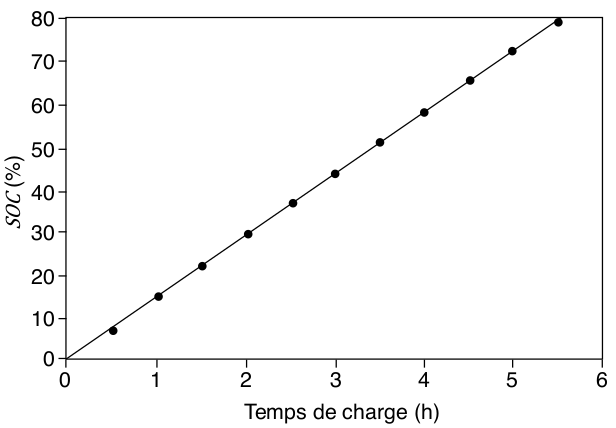
\includegraphics[width=6cm]{figures-Chp0/10-SoC.png}
\end{minipage}\hfill   
\begin{minipage}[c]{0.35\textwidth}     
    \captionof{figure}{\'{E}volution du SoC en fonction du temps de charge.}
    \label{fig:li-ion_car}
\end{minipage}
}

\exercice{
\Q Donner le signe de la puissance et du travail lorsqu'une cellule électrochimique est un récepteur reçoit de l'énergie. Même chose si il s'agit d'un générateur.

Dans les batteries, la puissance électrique est un critère de second plan. Ce qui intéresse principalement les industriels s'est que l'énergie délivrée par la batterie puisse stocker une grande quantité d'énergie, tout en la débitant de manière pérenne dans le temps.

\begin{center}
\begin{adjustbox}{width=0.95\textwidth}
\begin{tabular}{cccccc}
    \toprule
     \textbf{Technologie} & \textbf{Année de développement} & \textbf{Energie massique} & \textbf{Energie volumique} & \textbf{Tension} & \textbf{Cyclabilité}\\
     Unité & & \si{\watt\hour\per\kilo\gram} & \si{\watt\hour\per\liter} & \si{\volt}/au couple \ce{Li^+}/\ce{Li} & $\emptyset$ \\
     \midrule
     Plomb & 1859 & 35 & 70 & 2.0 & 200-250\\
     Nickel-Cadmium & 1900 & 60 & 100 & 1.2 & 400-500\\
     Nickel-Métal-Hydrure & 1975 & 80 & 240 & 1.2 & 400-500\\
     Lithium-Ion & 1978 & 250 & 400 & 3.6 & > 1000\\
     \bottomrule
\end{tabular}   
\end{adjustbox}
\captionof{table}{\small \'{E}volution des ordres de grandeurs de l'énergie massique, volumique, de la tension ainsi que de la cyclabilité d'une batterie en fonction de la technologie.}
\label{tab:battery_time}
\end{center}


\Q Commenter les valeurs de la Tab.\ref{tab:battery_time}. Quel est l'intérêt de la technologie Li-ion par rapport à d'autres technologies ?
\Q Mettre en relation ces données avec la place de l'élément Li au sein du tableau périodique.}

\exercice{
Les batteries utilisées couramment dans les véhicules électriques, mais également dans d'autres applications comme les téléphones portables, sont de type lithium-ion. Elles présentent l'avantage d'avoir une très grande énergie massique, comprise entre 90 et \SI{180}{\watt\hour\per\kilo\gram}. De plus, ces batteries, même partiellement déchargées, délivrent toujours la même puissance, ce qui permet une utilisation dans les mêmes conditions, quel que soit le niveau de charge. Le principe général d'une batterie lithium-ion est basé sur l'échange réversible des ions lithium entre une électrode positive en oxyde métallique (\ce{MO2}) et une électrode négative en graphite qui va stocker les ions lithium pendant la charge :

~

\begin{minipage}[c]{0.65\textwidth}
\centering
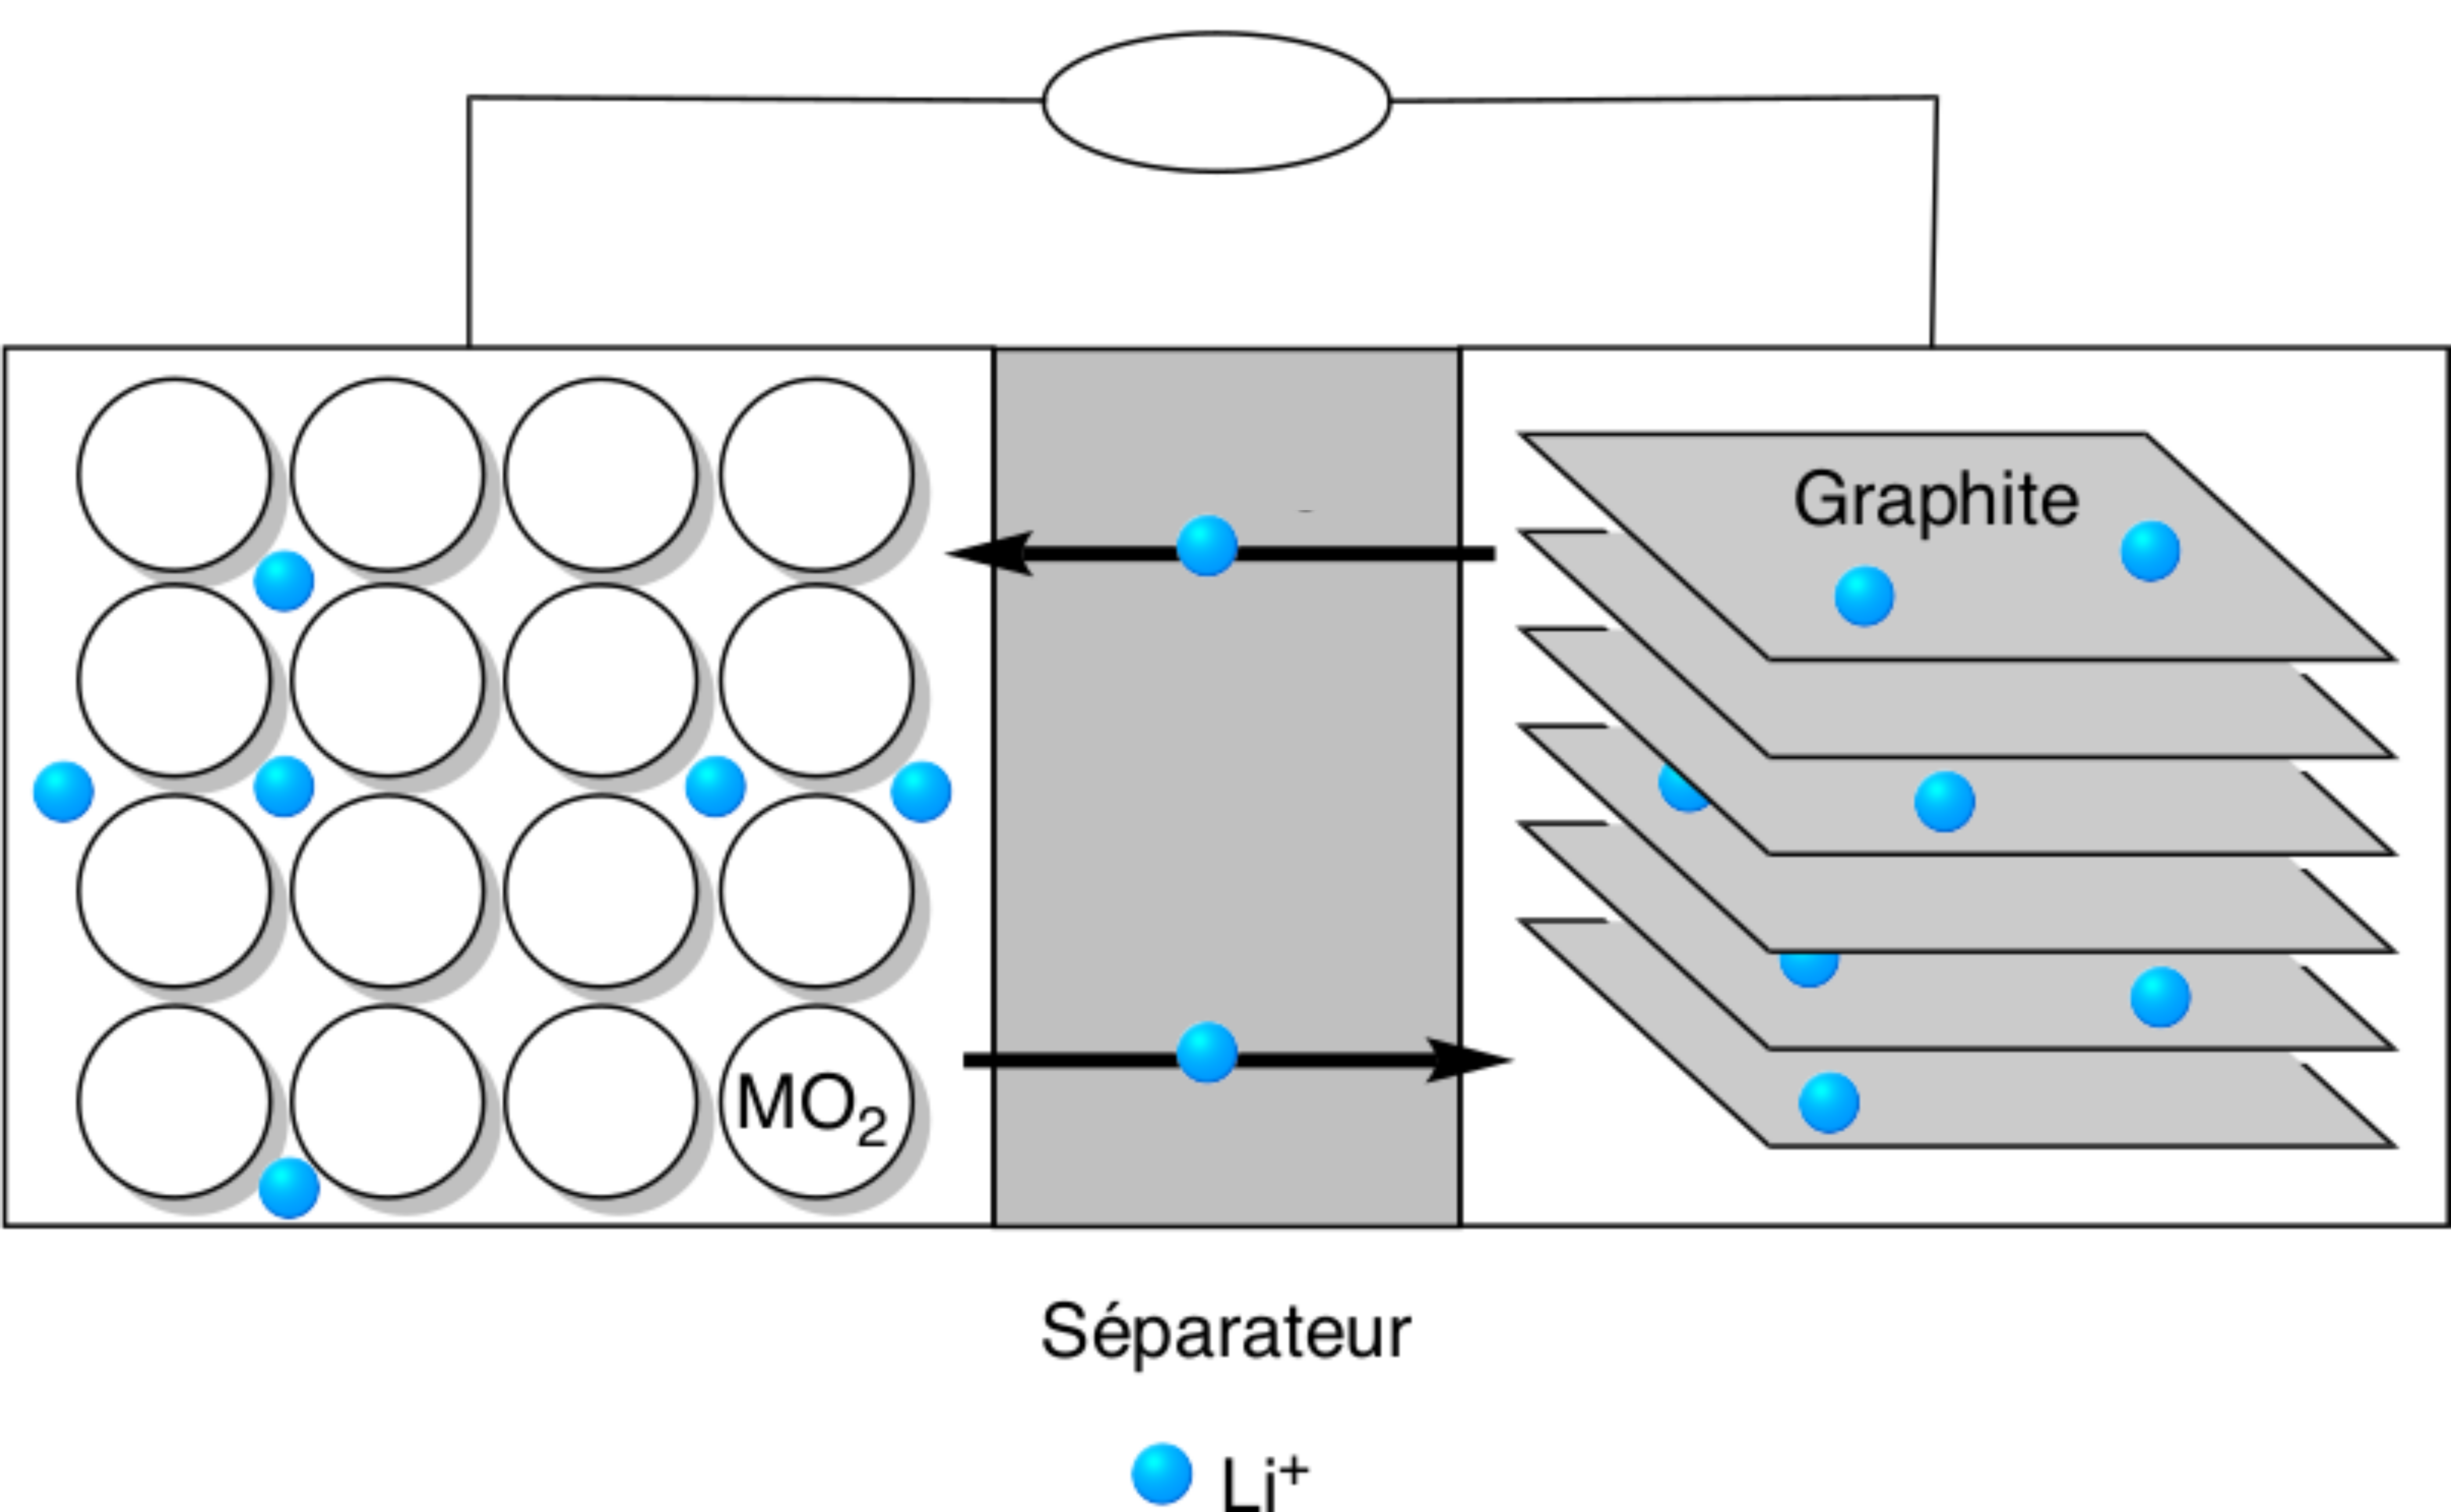
\includegraphics[width=6cm]{figures-Chp0/7-BatteryLithium.png}
\end{minipage}\hfill   
\begin{minipage}[c]{0.35\textwidth}     
\captionof{figure}{Technologie au lithium-ion. Le solvant utilisé est une espèce organique.}
\label{fig:li-ion}
\end{minipage}

\Q En vous appuyant sur la représentation du graphite, expliqué pourquoi les ions Li peuvent s'insérer entre les feuillets de graphite. On sait que le rayon ionique du lithium est de \SI{60}{\pico\meter} et le covalent est de \SI{134}{\pico\meter}.

\begin{minipage}[c]{0.65\textwidth}
\centering
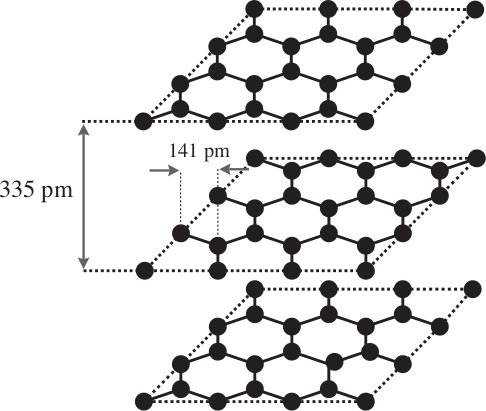
\includegraphics[height=4cm]{figures-Chp0/11-graphene.png}
\end{minipage}\hfill   
\begin{minipage}[c]{0.35\textwidth}     
\centering
\captionof{figure}{Structure du graphite}
\label{fig:graphite}
\end{minipage}

\Q A l'état totalement chargé, la structure du composé est \ce{LiC6}. Écrire la demi-équation rédox à cette électrode lors de la charge et de la décharge et préciser le signe de l'électrode de graphite.
La seconde électrode peut être en oxyde de cobalt (\ce{CoO2}) qui, après insertion des ions lithium,
forme l'oxyde lithié \ce{LiCoO2}. 
\Q Montrer que c'est l'élément cobalt qui change de degré d'oxydation ;
\Q Donner la demi-équation électronique associée au couple considéré lors de la charge et de la décharge
à cette électrode en précisant son signe.
\Q Reproduire et orienter le schéma de la Fig. \ref{fig:li-ion} dans le cas d'une charge puis d'une décharge. Vous indiquerez le nom et le signe des électrodes puis le flux d'électron, le courant électrique et la direction de migration des ions lithium.
%tiré de Mines-Pont 2022.

~

La suite de cet exercice sera traité à la partie suivante.}
\end{comment}

\def \FigPath{/home/jeff/Documents/IUTOrsay/1-Cours/3p06-Cours_Batterie/01-Cours/figures-Chp1/}
\graphicspath{{/home/jeff/Documents/IUTOrsay/1-Cours/3p06-Cours_Batterie/01-Cours/figures-Chp1/}}
\anachapter{Thermochimie à usage dans les batteries}
\label{chp:thermochimie}

\objectif{
\faBattery[0] Concepts généraux de thermochimie
\begin{itemize}[label=\faAngleRight]
\item Travail chimique et travail électrique ;
\item Différentielle totale exacte des fonctions d'états, relations entre les variables d'états conjuguées et les dérivées partielles premières des fonctions d'état ;
\item Expression intégrale de l'enthalpie libre ;
\item Expression de l'enthalpie libre de réaction ;
\item Potentiel chimique d'un gaz parfait et extension à tous les constituants.
\end{itemize}

\faBattery[2] Relation chimique fictive
\begin{itemize}[label=\faAngleRight]
\item Savoir utiliser des grandeurs de formation ou molaires pour établir les grandeurs de réaction ;
\item \'{E}tablir la relation entre grandeurs de réaction et force électromotrice ; 
\item Savoir discuter de l'influence de la température sur la force électromotrice.
\end{itemize}

\faBattery[4] Transfert de phase
\begin{itemize}[label=\faAngleRight]
\item \'{E}tablir l'expression de la différentielle de l'enthalpie libre entre deux phases s'échangeant des particules ;
\item \'{E}tablir l'expression liant la force électromotrice au potentiel chimique d'un constituant entre deux phases.
\end{itemize}
}

Contrairement aux systèmes thermodynamiques étudiés en première année, une cellule électrochimique ou batterie est un système \blancbis{fermé} capable de \blancbis{convertir} l'énergie chimique en énergie électrique (ou l'inverse). 

De ce fait, \blancbis{décrire mathématiquement} l'évolution de ces systèmes nécessite d'être capable de \blancbis{modéliser ces deux formes d'énergie}.

%\section{De l'énergie à la force électromotrice}

\section{Description d'une transformation chimique : le potentiel chimique}
Une batterie est un système thermodynamique fermé, qui \blancbis{reçoit ou donne} de l'énergie sous forme de \blancbis{chaleur}\mySideNote{\`{A} priori, vous avez dû remarquer que votre téléphone chauffait lors d'un usage intensif ou d'une charge sur secteur.} ou sous \blancbis{forme électrique} à l'extérieur.

De plus, les matériaux constituant les batteries forment un ensemble chimique complexe avec \blancbis{plusieurs} constituants chimiques, présents dans de \blancbis{multiples phases}. Prendre en compte cette complexité chimique rendra la description thermodynamique plus ardue que l'étude des systèmes de première année\mySideNote{Tous les outils introduis dans ce chapitre resserviront dans la suite de la scolarité et sont des concepts utilisables dans de nombreux contextes.}.

%Dans la suite, plusieurs notions nouvelles de thermodynamique qui réapparaitront tout au long de vos études\mySideNote{Tous les outils introduit dans ce chapitre reserviront dans la suite de la scolarité et sont des concepts extrêmement important pour tout individu voulant décrire rigoureusement la chimie.} permettant de décrire ces systèmes.

\subsection{Modélisation du système thermodynamique}

Afin de développer les principales formules, écrivons une forme générique d'équation de réaction comme : 

\begin{equation}
\nu_1 A_1 + \nu_2 A_2 + \ldots + \nu_N A_N = 0
\end{equation}

avec $\nu_k < 0$ (resp. $\nu_k > 0$) pour un réactif (resp. un produit).

Pour simplifier, on va considérer initialement que ce système est \blancbis{fermé} et comporte donc \blancbis{$N$ constituants} chimiques\mySideNote{$(A_1, A_2, \ldots A_N)$} dans une \blancbis{unique phase}. Ce système est mis en contact avec l'atmosphère (thermostat/barostat).

La réaction chimique est considérée comme une transformation monobare et monotherme.

\subsection{Travail chimique et potentiel chimique}

Le premier principe de la thermodynamique nous dit que pour un \blancbis{système physique}\mySideNote{Détente ou compression d'un gaz, échauffement d'un liquide$\ldots$} (sans réaction chimique), la variation d'énergie interne est dû aux échanges thermiques et au travail des forces de pression. Or, si on considère une transformation \blancbis{réversible}, le premier principe peut s'écrire comme\mySideNote{Si une transformation est réversible, alors 
\begin{align*}
\delta Q &\stackrel{\text{rev}}{=} T dS \\
\delta W_P &\stackrel{\text{rev}}{=} -P dV
\end{align*}
} : 
\begin{equation}
dU = T dS - P dV
\label{eq:PIT_phys}
\end{equation}



Par analogie avec la mécanique, il est possible de construire une grandeur analogue à la pression permettant de décrire l'évolution chimique d'un système. Cette grandeur, symboliée par la lettre $\mu$, est appelée potentiel chimique.

\begin{figure}[H]
\begin{minipage}{0.55\textwidth}
\subfloat[\label{fig:Chp1-02a}]{
\includegraphics[width=3cm]{Fig02a}}\hfill\subfloat[\label{fig:Chp1-02b}]{
\includegraphics[width=3cm]{Fig02b}}
\end{minipage}\hfill\begin{minipage}{0.40\textwidth}
\caption{\ref{fig:Chp1-02a} Représentation schématique de l'évolution d'un système mécanique composé de deux compartiments, séparé par une surface mobile, de volume $V_A$ et $V_B$, rempli de gaz à la pression $P_A$ et $P_B$ ; \ref{fig:Chp1-02b} Représentation schématique de l'évolution d'une réaction chimique \ce{{\color{blue} A} -> {\color{red}B}}.}
\end{minipage}
\end{figure}

Comme schématisé à la Fig. \ref{fig:Chp1-02a} la pression est la grandeur \blancbis{intensive} permettant de mesurer toutes les forces exercées par les particules de gaz de chacun des compartiments sur la surface mobile entre les compartiments A et B. La différence de pression permet donc de décrire l'évolution des volumes. Le potentiel chimique, représenté pour un système chimique à la Fig. \ref{fig:Chp1-02b}, est constuit de manière analogue.

Comme avec le travail des forces de pression, les thermodynamiciens définissent le travail chimique associé à chacun des constituants $j$ comme : 
\begin{equation}
\delta W_{\chi, j} \stackrel{rev}{=} \mu_j dn_j
\end{equation}

où $\mu_j$ est le potentiel chimique du constituant $j$.

\definition{
Le potentiel chimique représente "l'énergie potentielle" d'une mole de constituant $j$ dans le mélange au cours de la réaction chimique. 

~

Par analyse dimentionelle du travail, le potentiel chimique a pour unité \si{\joule\per\mole}.}



Pour un système, soumis à une transformation \blancbis{chimique réversible}, le premier principe permet d'écrire l'identité thermodynamique ci-dessous, dans laquelle a été ajouté le terme chimique à l'Eq. \ref{eq:PIT_phys} : 

\begin{equation}
dU = TdS - PdV + \sum_j \mu_j d n_j
\end{equation}
%par le système thermodynamique lorsqu'une mole de constituant est emmenée du vide dans une solution (solide, liquide).

%Il inclut le gain énergétique issu des interactions intermoléculaires et le gain entropique (augmntation du désordre) résultant de l'addition d'un constituant dans une phase.

\subsection{Forme différentielle des fonctions d'état}




\definition{
Dans le cas d'une transformation \blancbis{réversible} d'un système constitué de $N$ constituant chimique dans une phase, les identités thermodynamiques suivantes peuvent être écrites : 

\begin{align}
dU &= TdS - PdV + \sum_{j=1}^N \mu_j d n_j \label{eq:dU} \\
dH &= TdS + V dP + \sum_{j=1}^N \mu_j d n_j \label{eq:dH} \\
dG &= -S dT + V dP + \sum_{j=1}^N \mu_j d n_j \label{eq:dG}
\end{align}
}

Les fonctions d'états sont des fonctions à plusieurs variables : 

\begin{minipage}{0.45\textwidth}
\begin{tabular}{cc}
\toprule
Fonction d'état & Variables d'état \\
\midrule
U & $(S, V, n_1, \ldots, n_N)$ \\
H & $(S, P, n_1, \ldots, n_N)$ \\
G & $(T, P, n_1, \ldots, n_N)$ \\
\bottomrule
\end{tabular}
\end{minipage} \hspace{1cm} \begin{minipage}{0.45\textwidth}
\captionof{table}{Association de quelques fonctions d'état à leurs variables d'état naturelles.}
\end{minipage}

De ce fait, pour l'enthalpie libre, par exemple, on sait que l'on peut aussi écrire la différentielle totale exacte comme : 

\begin{equation}
dG = \left ( \frac{\partial G}{\partial T} \right )_{P, n_1, \ldots n_N} dT + \left ( \frac{\partial G}{\partial P} \right )_{T, n_1, \ldots n_N} dP + \sum_j \left ( \frac{\partial G}{\partial n_j} \right )_{T,P, n_{k \neq j}} d n_j
\label{eq:def_dG_totexact}
\end{equation}

On peut alors identifier avec la définition mathématique de la différentielle de G, Eq. \ref{eq:def_dG_totexact}, et le résultat issu du premier principe, Eq. \ref{eq:dG}, les dérivées suivantes\mySideNote{On peut lire que l'entropie est la variation de l'enthalpie libre avec la température lorsque la pression et la composition d'un mélange sont constants.} : 

\begin{center}
\begin{tabular}{ccc}
$\left ( \frac{\partial G}{\partial T} \right )_{P, n_1, \ldots n_N} = - S$ & $\left ( \frac{\partial G}{\partial P} \right )_{T, n_1, \ldots n_N} = V$ & $\left ( \frac{\partial G}{\partial n_j} \right )_{T,P, n_{k \neq j}} = \mu_j$ \\
\end{tabular}
\end{center}

Bien entendu, tout cela peut se résumer sur un tableau\mySideNote{Il est inutile d'apprendre ces dérivées par coeur, mais il faut savoir les retrouver facilement.} : 

\definition{
Les dérivées premières des fonctions d'état sont associées aux grandeurs, dites \blancbis{conjuguées}, des variables d'état de chaque fonction d'état. En écrivant la différentielle totale exacte et les résultats du premier principe de la thermodynamique, \blancbis{$3 (N + 2)$} dérivées premières peuvent être écrites : 
\begin{center}
\begin{tabular}{ccc}
$\left ( \frac{\partial U}{\partial S} \right )_{V, n_1, \ldots n_N} = T$ & $\left ( \frac{\partial U}{\partial V} \right )_{S, n_1, \ldots n_N} = -P$ & $\left ( \frac{\partial U}{\partial n_j} \right )_{S,V, n_k \neq n_j} = \mu_j$ \\
$\left ( \frac{\partial H}{\partial S} \right )_{P, n_1, \ldots n_N} = T$ & $\left ( \frac{\partial H}{\partial P} \right )_{S, n_1, \ldots n_N} = V$ & $\left ( \frac{\partial H}{\partial n_j} \right )_{S,P, n_k \neq n_j} = \mu_j$ \\
$\left ( \frac{\partial G}{\partial T} \right )_{P, n_1, \ldots n_N} = - S$ & $\left ( \frac{\partial G}{\partial P} \right )_{T, n_1, \ldots n_N} = V$ & $\left ( \frac{\partial G}{\partial n_j} \right )_{T,P, n_{k \neq j}} = \mu_j$ \\
\end{tabular}
\end{center}} 

\subsection{Définition intégrale de l'enthalpie libre}

\definition{Dans un système chimique composé de $N$ constituants, l'enthalpie libre est une fonction extensive définit sous forme intégrale par : 

\begin{equation}
G(T, P, n_1, .... n_N) = \sum_{j=1}^N \mu_j n_j
\end{equation}}

Une façon de parvenir intuitivement à ce résultat, est de se souvenir que l'enthalpie libre est une fonction \textbf{extensive}, c'est-à-dire que si je prends un système chimique et que je multiplie sa taille par deux, l'enthalpie libre est multipliée par deux.

\begin{minipage}{0.55\textwidth}

\includegraphics[width=8cm]{Fig03}
\end{minipage}\hfill\begin{minipage}{0.40\textwidth}
\captionof{figure}{Multiplication par deux d'un système chimique composé de deux constituants chimiques.}
\end{minipage}

Si on prend un système chimique quelconque et qu'on l'agrandit $\lambda$ fois, on s'attend à ce que l'enthalpie augmente $\lambda$ fois, soit l'égalité : 
\begin{equation}
G(T, P, \lambda n_1, .... \lambda n_N) = \lambda G(T, P, n_1, .... n_N)
\end{equation}

Naturellement, on en déduit alors que :
\begin{equation}
G(T, P, n_1, .... n_N) = \sum_j \mu_j n_j
\end{equation}

\subsection{Relation entre grandeurs de réaction et potentiel chimique}

\definition{
L'enthalpie libre de réaction est liée aux potentiels chimiques par la relation : 
\begin{equation}
\Delta_r G = \sum_j \nu_j \mu_j 
\end{equation}
}

Pour démontrer cette relation, il faut se rappeler qu'il est possible de décrire l'évolution du système lors d'une réaction chimique grâce à une unique variable : l'avancement chimique $\xi$, au lieu de considérer individuellement la variation de composition de chacun des constituants. Pour cela, dressons un tableau d'avancement : 

\begin{tabular}{cccccccc}
\toprule
 & $\nu_1 \ce{A_1}$ & + &  $\nu_2 \ce{A_2}$ & + & $\ldots$ & + & $\nu_N \ce{A_N}$ = 0 \\
\midrule
$t = 0$ & $n_1(0)$ & & $n_2(0)$ & & $\ldots$ & & $n_N(0)$ \\
$t > 0$ & $n_1(0) + \nu_1 \xi (t)$ & & $n_2(0) + \nu_2 \xi (t)$ & & $\ldots$ & & $n_N(0) + \nu_N \xi (t)$ \\
\bottomrule
\end{tabular}

On voir immédiatement que la seule variable temporelle $\xi$, d'où
\begin{align}
n_j (t) = n_j (0) + \nu_j \xi (t) \implies dn_j = \nu_j d\xi \label{eq:dnj}
\end{align}

Or, on peut écrire la première identité thermodynamique Eq. \ref{eq:dG} en y intégrant l'équation Eq. \ref{eq:dnj} : 

\begin{equation}
dG = -S dT + V dP + \left( \sum_j \nu_j \mu_j \right) d \xi
\end{equation}

Vous savez que par définition, l'enthalpie de réaction représente la variation de l'enthalpie libre avec l'avancement, soit : 

\begin{equation}
\Delta_r G = \left( \frac{\partial G}{\partial \xi } \right)_{T, P} \implies \Delta_r G = \sum_j \nu_j \mu_j
\end{equation}

\section{Expression, propriétés et utilisation du potentiel chimique}

\subsection{Expression}

\definition{
Le potentiel chimique d'un constituant $i$ dans une phase donnée est décrit par la forme analytique : 

\begin{equation}
\mu_i (T, P, a_i) = \mu_i^\circ (T) + RT \ln a_i
\end{equation}

où $a_i$ l'activité du constituant et $\mu_i^\circ$ est le potentiel chimique dans son état standard.}

Le potentiel chimique a une forme fonctionnelle inspirée d'un gaz parfait. Considérons un gaz parfait (nécessairement constitué d'une phase) constitué de $N$ constituants à la pression P et la température T. Le potentiel chimique du constituant $i$ est donné par : 

\begin{equation}
\mu_j = \left ( \frac{\partial G}{\partial n_j} \right )_{T,P, n_i \neq n_j}
\end{equation}

Dans le cas d'un gaz parfait, on peut montrer que : 

\begin{align}
\mu_j (T, P, x_j) &= \mu_j^\circ (T) + RT \ln \frac{P_j}{P^\circ} \\
&= \mu_j^\circ (T) + RT \ln x_j + RT \ln \frac{P}{P^\circ}
\end{align}

avec $P_i$ la pression partielle du gaz $i$ et $x_i$ la fraction molaire.

\example{
On sait qu'un gaz est constitué de $N$ constituants tel que : 
\begin{align}
\frac{\partial \mu_i}{\partial P} &=  \frac{\partial}{\partial P} \frac{\partial G}{\partial n_i} \\
&= \frac{\partial}{\partial n_i} \frac{\partial G}{\partial P} \quad \text{(car G est une fonction d'état)}\\
&= \frac{\partial}{\partial n_i} V \\
&= V_{m, i}
\end{align}

Or si les constituants sont des gaz parfaits, on sait que : $P_i V_{m,i} = RT$, d'où : 

\begin{align}
\frac{\partial \mu_i}{\partial P} &= \frac{RT}{P_i} \\
\int_{\mu_i^\circ (T)}^{\mu_i (T, P_i)} d\mu_i &= \int_{P^\circ}^{P_i} \frac{RT}{P'_i} d P'_i \\
\mu_i (T, P_i) - \mu_i^\circ (T) &= RT \ln \frac{P_i}{P^\circ}
\end{align}}

\subsection{Résultats importants}

\subsubsection{Influence de la température}

\definition{
Le potentiel chimique est une fonction de la température, dont la variation avec celle-ci est donnée par l'opposé de l'entropie molaire du constituant $j$ :

\begin{align}
\left( \frac{\partial \mu_j }{\partial T} \right)_{P, n_1, \ldots , n_N}= -S_{m,j}
\end{align}
}

Une simple étude de la valeur de l'entropie molaire d'un constituant vous permet donc de savoir à quel point celle-ci va diminuer l'énergie potentielle d'un constituant chimique.


\subsubsection{Expression de l'enthalpie libre de réaction}

\definition{
L'enthalpie de réaction est liée au quotient réactionnel $Q_r$ par la relation : 

\begin{equation}
\Delta_r G = \Delta_r G^\circ + RT \ln Q_r
\end{equation}


où $\Delta_r G^\circ$ est l'enthalpie standard de réaction, $T$ la température et $Q_r$ le quotient réactionnel.
}

Cette relation admise en BUT1 est un résultat très utile qui est une conséquence directe de la forme analytique du potentiel chimique.

\example{
On sait que :

\begin{equation}
\Delta_r G = \sum_i \nu_i \mu_i 
\end{equation}

On a alors : 

\begin{align}
\Delta_r G &= \sum_i \nu_i (\mu_i^\circ + RT \ln a_i) \\
 &= \sum_i (\nu_i \mu_i^\circ + RT \nu_i \ln a_i) \\
 &= \sum_i \nu_i \mu_i^\circ + RT \sum_i \ln a_i^{\nu_i} \\
 &= \underbrace{\sum_i \nu_i \mu_i^\circ}_{\Delta_r G^\circ} + RT \ln \underbrace{\prod_i a_i^{\nu_i}}_{Q_r}
\end{align}
}


\subsection{Application aux batteries : le transfert de phase}
%Warning Fig.

Le potentiel chimique est une grandeur particulièrement utile dans l'étude des batteries. En effet, il permet le plus souvent de ramener un problème complexe constitué de $N$ constituants chimique à l'étude de $N$ problèmes simple à $1$ constituant. Ainsi, à l'aide de cette grandeur, les chimistes des matériaux s'affranchissent de toute difficulté dans l'étude de leurs systèmes.

Dans une batterie, lors d'une décharge, on sait que deux phénomènes ont lieu simultanément : 
\begin{enumerate}
\item les électrons migrent du pôle $\ominus$ (anode) au pôle $\oplus$ (cathode) par les fils électriques ;
\item les cations migrent du pôle $\ominus$ au pôle $\oplus$ par l'électrolyte.
\end{enumerate}

Les chimistes des matériaux ramènent souvent l'étude complexe d'une réaction d'oxydoréduction au transport d'une espèce chimique.

\subsubsection{\'{E}tude de l'équilibre chimique}

On va formaliser les deux problèmes physiques ci-dessus de manière unique : une espèce \emph{A} migre de l'électrode $\oplus$ vers l'électrode $\ominus$ en passant par un milieu matériel, noté $m$.

\begin{minipage}{0.45\textwidth}

\includegraphics[width=6cm]{Fig04}
\end{minipage}\hfill\begin{minipage}{0.45\textwidth}
\captionof{figure}{Modélisation d'un transfert d'électron ou d'un transfert d'ion.}
\label{fig:Chp1-04}
\begin{equation*}
\ce{A(\oplus) <=> A(m) <=> A(\ominus)}
\end{equation*}
\end{minipage}

On sait que lors de l'étude d'un tel transfert, le système est composé de $N$ constituants répartis, cette fois-ci, \blancbis{plusieurs} phases. L'ensemble forme un système \emph{fermé}, mais il peut y avoir un \blancbis{transfert de matière} entre les différentes phases, comme illustré dans la Fig. \ref{fig:Chp1-04}.

Si on considère un transfert d'un constituant A entre les deux électrodes, le milieu matériel n'étant qu'un médiateur permettant ce transport, l'enthalpie libre, se réécrit alors comme : 
\begin{equation}
dG = -S dT + V dP + \sum_j \mu_j^\oplus dn_j^\oplus + \sum_j \mu_j^\ominus dn_j^\ominus
\end{equation}

En général, il va de soi que le milieu matériel ne constitue pas un "réservoir"\mySideNote{Un fil électrique ne permet pas de stocker des électrons par exemple} permettant de stocker les espèces qui migrent. On a alors nécessairement une équation de conservation de la matière : 
\begin{equation}
n_j^{tot} = n_j^\oplus + n_j^\ominus + n_j^m \implies dn_j^\oplus + dn_j^\ominus = 0
\end{equation}

qui permet de réduire l'enthalpie libre à : 
\begin{equation}
dG = -S dT + V dP + \sum_j (\mu_j^\oplus - \mu_j^\ominus) dn_j^\oplus
\end{equation}

\definition{On considère une transformation thermostatée et barostatée où une espèce \ce{A} migre du pôle $\oplus$ vers $\ominus$ suivant l'équation de réaction : 
\begin{align*}
\ce{A ( \oplus) <=> A (\ominus) }
\end{align*}

La variation d'enthalpie libre peut s'écrire : 


\begin{equation}
dG = \sum_j (\mu_j^\oplus - \mu_j^\ominus) dn_j^\oplus
\label{eq:dG_phasetransfert}
\end{equation}
}


\subsubsection{Conséquence}

Le second principe de la thermodynamique nous dit que pour une transformation monobare/monotherme (en l'absence de travail électrique), l'enthalpie libre décroit, soit que $dG < 0$. La relation Eq. \ref{eq:dG_phasetransfert} nous montre que : 
\begin{itemize}
\item $\mu_j^\oplus > \mu_j^\ominus$ le constituant $j$ est soumis à une "force chimique" qui le pousse à aller de l'électrode $\oplus$ à l'électrode $\ominus$ ; 
\item $\mu_j^\oplus < \mu_j^\ominus$ le constituant $j$ est soumis à une "force chimique" qui le pousse à aller de l'électrode $\ominus$ à l'électrode $\oplus$ ; 
\item $\mu_j^\oplus = \mu_j^\ominus$ le constituant $j$ est soumis à aucune force chimique.
\end{itemize}

Par force chimique qui le pousse à aller de l'électrode $\oplus$ à l'électrode $\ominus$, il est sous-entendu que le constituant $j$ est plus stable chimiquement dans la phase $\ominus$ et $\oplus$. Cette affinité chimique pour une phase plutôt que l'autre peut-être vu comme une force thermodynamique\mySideNote{Par analogie avec la force en mécanique.}.


\section{Travail électrique}

Tout le travail de construction du potentiel chimique nous a permis de montrer que le potentiel chimique constitue une mesure de la stabilité d'un constituant $j$ dans sa phase. Bien entendu, les espèces considérées dans une pile seront souvent \blancbis{chargées} et le travail électrique devra donc aussi être considéré dans le second principe.


\subsection{Définition}
Nous avons vu au chapitre précédent que le travail électrique, notée $W'$, s'écrit mathématiquement comme : 
\begin{equation}
W' = \int e dq
\end{equation}

où $e$ est la f.e.m. et $dq$ la variation de charge du système.

Afin de décrire ce système, on va considérer une forme plus habituelle de l'équation de réaction au sein de la cellule : 
\begin{align*}
\nu_1 A_1^{z_1} + \nu_2 A_2^{z_2} + \ldots + \nu_N A_N^{z_N} = 0
\end{align*}

où $(z_1, z_2 \ldots z_N)$ sont les charges formelles associées à chacune des entités rédox. De plus, on va considérer que $m e^-$ sont échangés entre les deux pôles de la cellule. 

\attention{Il est important de noter dès à présent que l'électron est une entité qui sera considérée à part par rapport aux autres constituants chimiques à présent. L'Eq. \ref{eq:dG_phasetransfert} sera réécrite : 
\begin{align*}
dG = \sum_j (\mu_j^\oplus - \mu_j^\ominus) \cdot dn^\oplus_j + ( \mu_e^\oplus - \mu_e^\ominus ) \cdot dn_e^\oplus
\label{eq:dG_phasetransfert_2}
\end{align*}}


\subsection{Relation à l'enthalpie libre}
Dans le cas d'une transformation chimique soumis à un travail électrique, le second principe de la thermodynamique permet d'écrire : 

\begin{equation}
dG = \delta W' = e dq
\end{equation}

Or si on s'intéresse à la variation de charge $dq$ au pôle $\oplus$, on peut écrire par exemple que : 
\begin{equation*}
dq = \sum_i (-z_i F) \cdot dn^\oplus_i - F \cdot dn^\oplus_e
\end{equation*}

On a alors une égalité intéressante entre le terme chimique et le terme électrique lorsque l'on est à l'équilibre chimique :
\begin{equation}
\sum_j (\mu_j^\oplus - \mu_j^\ominus) \cdot dn^\oplus_j + ( \mu_e^\oplus - \mu_e^\ominus ) \cdot dn_e^\oplus = \sum_i (- z_i F e) \cdot  dn^\oplus_i - F e \cdot dn^\oplus_e
\end{equation}

\definition{
On considère une transformation monobare et monotherme d'un système chimique composé de $N$ constituants où un échange de $m$ électrons a lieu entre deux électrodes. \`{A} l'équilibre chimique, on peut écrire pour chacun des constituants chimiques l'égalité suivante :

\begin{align*}
\mu_j^\oplus - \mu_j^\ominus = - z_j F e
\end{align*}

et écrire pour les électrons que : 

\begin{align*}
\mu_e^\oplus - \mu_e^\ominus = - F e
\end{align*}
}

L'un des points essentiels à noter dès à présent que la f.e.m. est une grandeur \blancbis{centrale} dans la description des cellules électrochimiques : sa simple valeur nous indique la stabilité de n'importe quel constituant chimique dans les différentes phases d'une cellule électrochimique. Or, la f.e.m. est liée à la réaction "fictive" de la cellule.


\begin{comment}
Or, en général, on cherche à décrire l'évolution de la charge avec la même variable que la partie chimique : l'avancement $\xi$.
\begin{equation}
dG = - z F e d\xi 
\end{equation}

\begin{boxedminipage}[t]{15cm}
On écrit la demi-équation rédox : 
\begin{equation}
\ce{Ox_1 = Red_1^{z+} + z e^-}
\end{equation}

On peut alors dresser un tableau d'avancement à partir de l'anode :
\begin{center}
\begin{tabular}{cccccccc}
\toprule
$t$ & \ce{Ox_1} & \ce{ = } & \ce{Red_1^{z+}} & + & \ce{z e^-} & Charges émis & Charges reçues \\
\midrule
$t=0$ & $n_0$ & & 0 & & 0 & 0 & 0\\
$t=\infty$ & $n_0 - \xi$ & & $n_0 + \xi$ & & $z \xi$ & $z F \xi$ & $-z F \xi$ \\
\bottomrule
\end{tabular}
\end{center}

On peut alors montrer que la variation de la quantité de charge reçue est donnée par : 
\begin{equation}
dq = F \cdot (-z d \xi) = -z F d\xi
\end{equation}

On a alors à partir du travail électrique, une nouvelle expression donnée par : 

\begin{equation}
dG = -z F e d\xi
\end{equation}
\end{boxedminipage}

\definition{Dans un système à pression et température constante, il est possible de lier l'enthalpie de réaction définie à l'Eq. \ref{} à la force électromotrice du système : 

\begin{equation}
\Delta_r G = -z F e
\end{equation}}

Dans ce genre de relation, on pose pour un système reversible, une juste proportionnalité entre la tension électrique du système et la variation d'énergie chimique au sein de deux demi-piles.
\end{comment}

\section{Réaction fictive d'une cellule électrochimique et force électromotrice}

\subsection{Relation entre l'enthalpie de réaction et la f.e.m.}

\definition{Dans une cellule électrochimique, dans laquelle on peut écrire une équation de réaction "fictive" de la forme :
\begin{equation}
\ce{\nu_1 A_1^{z_1} + \nu_2 A_2^{z_2} + \dots \nu_N A_N^{z_N} = 0}
\end{equation}

Dans une telle réaction, la variation d'enthalpie libre avec l'avancement est donnée par l'enthalpie libre de réaction $\Delta_r G$. Si on considère une transformation monobare et monotherme, la f.e.m. de la réaction est liée directement à l'enthalpie de réaction par la relation :

\begin{equation}
\Delta_r G = -m F e
\label{eq:DrG_fem}
\end{equation}

où $m$ est le nombre d'électrons échangé entre les pôles de la cellule.
}

On sait que l'enthalpie libre associée à un système thermostaté et barostaté, où un transformation chimique a lieu, peut s'écrire à l'aide des variables d'état $(T, P, \xi)$. 

L'enthalpie libre d'une telle réaction s'écrit : 
\begin{align*}
dG = -S dT + V dP + \Delta_r G d \xi
\end{align*}

De ce fait, si cette réaction reçoit un travail électrique $\delta W'$, on peut alors utiliser le second principe de la thermodynamique : 

\begin{align*}
dG \stackrel{\text{rev}}{=} -m F e d\xi
\end{align*}

\`{A} (T, P) constant, on en déduit alors l'Eq. \ref{eq:DrG_fem}.


\subsection{Relation entre f.e.m. et grandeurs de référence}

La relation \ref{eq:DrG_fem} est très utile car elle permet d'établir une relation simple entre l'enthalpie libre de la réaction "fictive" de la cellule électrochimique et la f.e.m. de la cellule.

En $BUT1$, les lois de Hess ont été établies afin de lier la détermination des grandeurs standard de n'importe quelle réaction aux réactions de formation des constituants de la réaction.

\subsubsection{Utilisation de la loi de Hess}

La loi de Hess permet de remonter aux grandeurs de réaction à partir de valeurs tabulées : l'enthalpie de formation standard $\Delta_f H^\circ$ et l'entropie molaire standard $S_m^\circ$.

\begin{align}
\Delta_r H^\circ &= \sum_j \nu_j \Delta_f H_j^\circ \\
\Delta_r S^\circ &= \sum_j \nu_j S_{m,j}^\circ \\
\Delta_r G^\circ &= \sum_j \nu_j \Delta_f G_j^\circ
\end{align}

Ces lois de Hess permettent de remonter à la force électromotrice $e^\circ$ dans des conditions standard : 

\begin{equation}
e^\circ (T) = - \frac{\Delta_r G^\circ}{mF}
\end{equation}

\exercice{
Dans le domaine médical, la pile $\ominus ~ \ce{Li} | \text{electrolyte} | \ce{I_2} ~ \oplus$ est utilisée comme source d'énergie pour les pacemakers. 

\Q Donner les demi-équations rédox associées à l'anode et la cathode, et en déduire l'équation de réaction.
\Q Calculer l'enthalpie standard de réaction à \SI{298}{\kelvin}.
\Q Calculer l'entropie standard de réaction à \SI{298}{\kelvin}.
\Q En déduire l'enthalpie libre de réaction à \SI{298}{\kelvin} puis déterminer la f.e.m dans ces conditions.

Dans ce dispositif, la tension de sortie a été mesurée en fonction de la quantité de charge déchargée. 

\begin{minipage}{0.55\textwidth} 

\includegraphics[width=\textwidth]{Fig06}
\end{minipage} \hfill \begin{minipage}{0.40\textwidth} 
\captionof{figure}{\'{E}volution de la tension de sortie et de la résistance interne d'une batterie \ce{Li}/\ce{I2} utilisée dans les pacemakers.}
\label{fig:Chp1-06}
\end{minipage}

\Q Montrer l'accord entre vos grandeurs et la mesure sur la majorité du cycle de décharge de la pile. 
\Q En vous appuyant sur l'équation de réaction, lier l'écroulement du potentiel de réaction au-delà de \SI{1.2}{\ampere\hour} à la structure de la pile.

~

\textbf{Données}
\begin{center}
\begin{tabular}{ccccc}
 & & Li & \ce{I2} & \ce{LiI} \\
Enthalpie de formation & [\si{\kilo\joule\per\mole}] & 0 & 0 & -270.1\\
Entropie molaire & [\si{\joule\per\mole\per\kelvin}] & 29.08 & 116.14 & 85.77 \\
\end{tabular}
%Table 2.1, advanced battery.
\end{center}}


\subsubsection{\'{E}tude de l'influence de la température}

Dans les cellules électrochimiques, l'étude de l'influence de la température est extrêmement importante pour comprendre la tenue thermique d'une cellule. Les lois de Hess permettent de remonter à la force électromotrice $e^\circ$ dans des conditions standard : 

\begin{equation}
e^\circ (T) = \frac{\Delta_r S^\circ}{mF} T - \frac{\Delta_r H^\circ}{mF}
\end{equation}

Pour une variation modérée de température, on peut souvent se placer dans l'approximation d'Ellingham, ce qui permet d'écrire que : 

\begin{equation}
\frac{d e^\circ}{dT} = \frac{\Delta_r S^\circ}{mF}
\end{equation}

Cette grandeur est appelée c{\oe}fficient thermique de la cellule.

\exercice{
On se placera dans l'approximation d'Ellingham.
\Q En déduire la relation entre la variation de la force électromotrice $e^\circ$ avec la température.
\Q Commenter et justifier la valeur obtenue.}

\subsection{D'où vient la relation de Nernst ?}

En supposant un système réversible, composé d'une pile fictive suivante : 

\begin{equation}
\ominus \quad \ce{Pt (s)} | \ce{Ox_1 (\phi)}; \ce{Red_1 (\phi)} || \ce{H^\oplus (aq)} | \ce{H2 (g)} | \ce{Pt (s)} \quad \oplus
\label{eq:pileOxRedvsESH}
\end{equation}
où $\phi$ indique la phase et \ce{Ox_1}/\ce{Red_1} indique un couple oxydant/réducteur quelconque. L'équation de réaction de cette pile est donnée par : 

\begin{center}
\begin{minipage}{0.4\textwidth}
\begin{align*}
\ce{Red_1 (\phi) &= Ox_1 (\phi) + m e^-} \\
\ce{H^+ (aq) + e^- &= H_2 (aq)} \quad \times m \\
\hline
\ce{m H^+ (aq) + Red_1 (\phi) &= \frac{m}{2} H_2 (g) + Ox_1 (\phi)}
\end{align*}
\end{minipage}
\end{center}

Dans ce système, la cathode est une électrode standard à hydrogène (ESH)

\begin{align}
\underbrace{\Delta_r G}_{-m F e} & = \underbrace{\Delta_r G^\circ}_{-m F e^\circ} + RT \ln Q_r \\
e &= e^\circ - \frac{RT}{mF} \ln Q_r \\
\end{align}

Or on sait que la force électromotrice est donnée par : 
\begin{align}
e &= E_\oplus - E_\ominus \\
&= E ( \ce{H^+} / \ce{H2} ) - E ( \ce{Ox_1} / \ce{Red_1} )
\end{align}

Or, on sait que l'ESH, référence absolue des potentiels, est définie par les hypothèses suivantes :
\begin{itemize}
\item $E^\circ ( \ce{H^+} / \ce{H2} ) = 0 $ (convention de Latimer) ;
\item l'activité du proton vaut 1 : $a (\ce{H^+}) = 1$ ;
\item l'activité du dihydrogène vaut 1 $a (\ce{H2}) = 1$.
\end{itemize}

Dans ces conditions, le potentiel cathodique vaut $E_\oplus = E ( \ce{H^+} / \ce{H2} ) = 0 $ ce qui sert de référence à tous les potentiels d'électrodes. Dans ce système, on retrouve alors l'équation de Nernst qui permet de retrouver le potentiel d'électrode par rapport au couple \ce{H^+}/\ce{H2}.

\definition{
Le potentiel d'électrode est donné par l'équation de Nernst définie comme : 
\begin{equation}
E ( \ce{Ox_1} / \ce{Red_1} ) = E^\circ ( \ce{Ox_1} / \ce{Red_1} ) + \frac{RT}{mF} \ln \frac{a^{|\nu_{Ox}|}(\ce{Ox_1})}{a^{|\nu_{Red}|}(\ce{Red_1})}
\end{equation}
où $m$ indique le nombre d'électrons échangés.}

\newpage

\definition{
\begin{center}
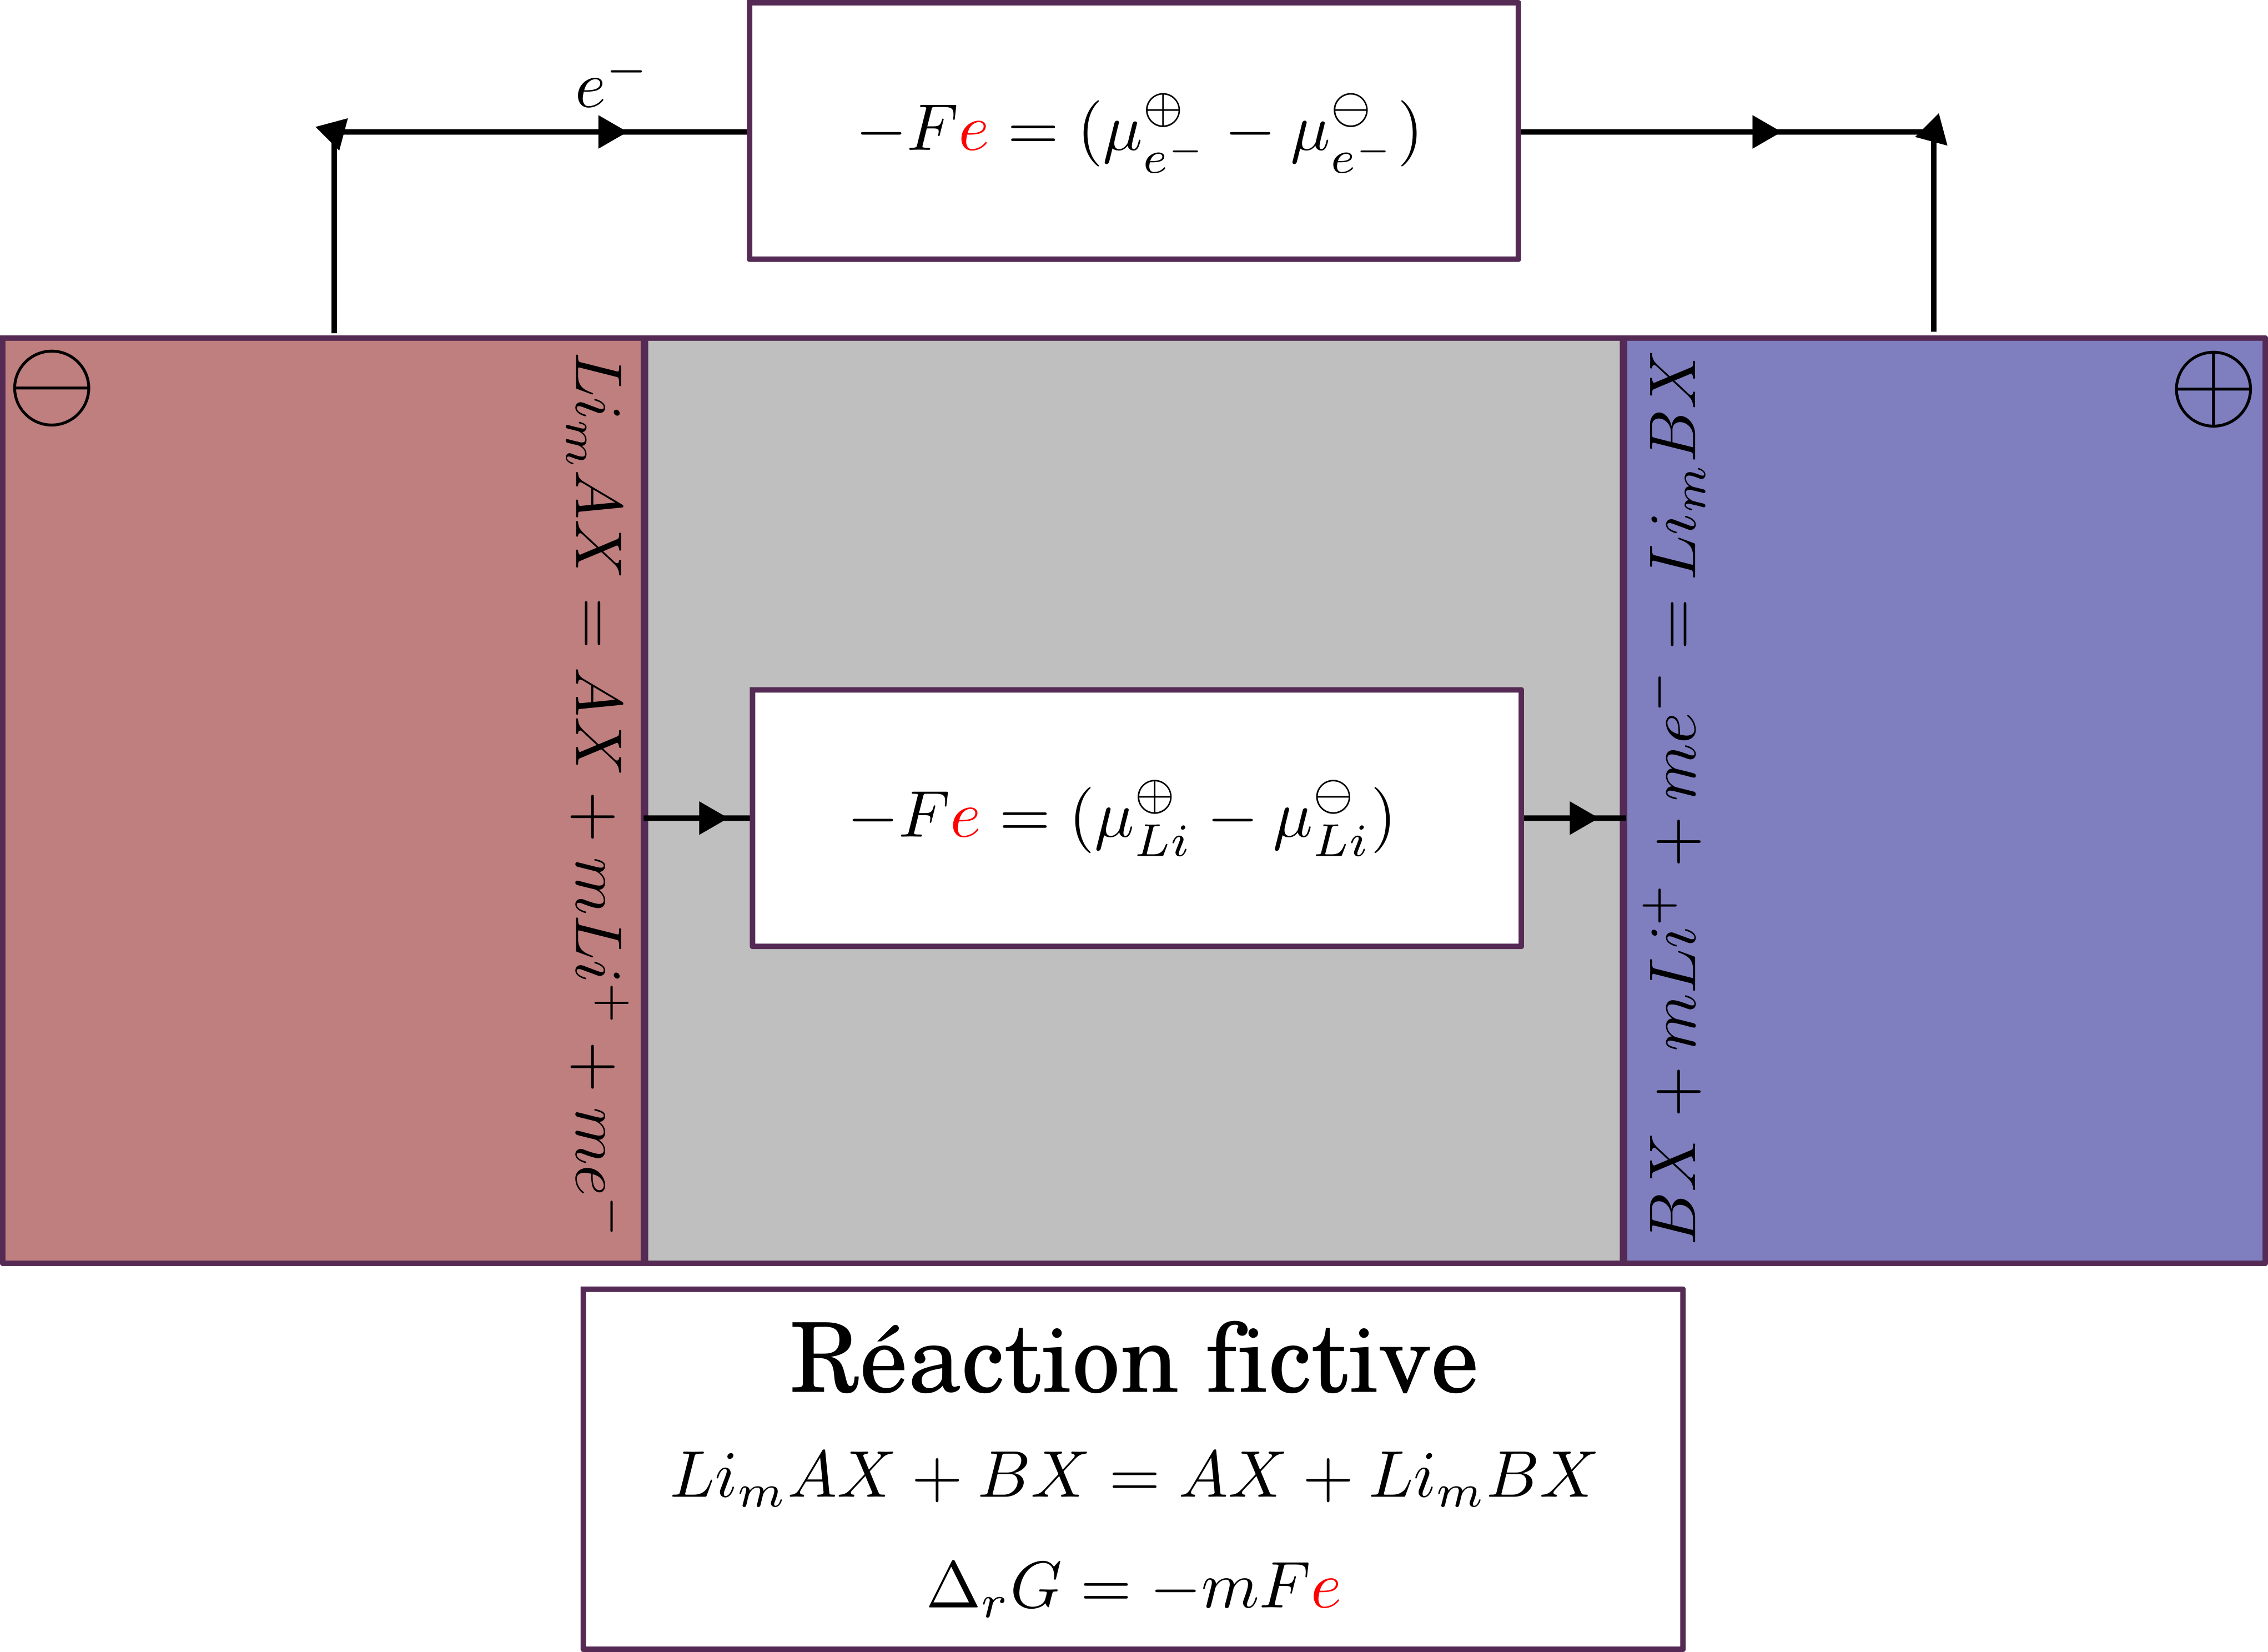
\includegraphics[width=0.8\textwidth]{figures-Chp1/Fig07}
\captionof{figure}{Résumé des relations clefs, utilisés dans le domaine des batteries, lors de la décharge d'un accumulateur au lithium composé de deux matériaux d'insertion aux pôles.}
\end{center}
Dans ce chapitre, on est parvenu à montrer que la force électromotrice est la grandeur thermodynamique qui permet de relier trois phénomènes : 
\begin{itemize}
\item la réaction fictive ;
\item le "transfert de phase" de l'électron ;
\item le "transfert de phase" du lithium.
\end{itemize}
Ces différentes relations, comme nous le verrons aux chapitres suivants, sont autant de points de vue possibles pour un chimiste d'interpréter les phénomènes chimiques à l'origine des variations de la f.e.m. 
}

%https://www.youtube.com/watch?v=7Wds1UdtOqc&ab_channel=PhysicalChemistry
\begin{comment}
\exercice{Donner la variance de quelques systèmes solides :
\begin{itemize}
\item donner la variance d'un alliage de bronze (solution solide de Cu et Zn)

\begin{boxedminipage}[t]{15cm}
\begin{align*}
X =4 &: P, T, \mu_{Cu}, \mu_{Zn} \\
Y =3 &: \text{1 phase solide} \\
v &= 3
\end{align*}
Un bronze stable est décrit à l'équilibre par (P, T, $x_{Cu}$).
\end{boxedminipage}

\end{itemize}}



\begin{boxedminipage}[t]{15cm}
Prenons-le cas de la pile $\ominus ~ \ce{Li} | \text{electrolyte} | \ce{I_2} ~ \oplus$, on peut alors écrire les différentes phases : 

On peut alors interpréter l'enthalpie libre de réaction par : 
%\begin{equation}
%\Delta_r G^\circ = \mu (\ce{LiI}) - \mu(\ce{Li}) - \frac{1}{2} \mu ( \ce{\LiI} )
%\end{equation}

\end{boxedminipage}
\end{comment}


%https://www.youtube.com/watch?v=4-1psMHSpKs&ab_channel=TheLimitingFactor

%https://www.college-de-france.fr/fr/agenda/cours/electrochimie-appliquee-les-differents-systemes-de-batteries/la-technologie-ion-lithium-son-origine-son-evolution-ses-dernieres-avancees-et-son-futur

%https://www.youtube.com/watch?v=DBLHaLhyo2w&ab_channel=BillyWu


\def \FigPath{/home/jeff/Documents/IUTOrsay/1-Cours/3p06-Cours_Batterie/01-Cours/figures-Chp4/}
\graphicspath{{/home/jeff/Documents/IUTOrsay/1-Cours/3p06-Cours_Batterie/01-Cours/figures-Chp4/}}
\anachapter{Force électromotrice \& relation aux matériaux}
\label{chp:fem}

\objectif{
\faBattery[0] Mesure de la f.e.m.
\begin{itemize}[label=\faAngleRight]
\item Principe, intérêt et limites du titrage coulométrique ;
\item Utiliser la variance et la variance particulière pour étudier les degrés de liberté d'un système.
\end{itemize}

\faBattery[2] \'{E}tude des systèmes binaires et ternaires
\begin{itemize}[label=\faAngleRight]
\item Interpréter ou construire un profil de potentiel issu d'un titrage coulométrique ;
\item Lier la force électromotrice aux grandeurs de réaction à différentes compositions dans un système à deux ou trois constituants de variance nulle ;
\item Calculer la capacité spécifique théorique et l'énergie théorique maximale ; 
\item Interpréter l'évolution du potentiel d'électrode dans un système de variance non nulle à l'aide du potentiel chimique.
\end{itemize}

\faBattery[4] Courbe de charge-décharge
\begin{itemize}[label=\faAngleRight]
\item Justifier l'origine de la différence de potentiel entre un système à courant nul et à courant constant ;
\item Expliquer l'origine de l'hystérèse entre charge et décharge à l'aide de la thermodynamique et mettre en relation avec les phénomènes microscopiques ;
\item Connaître et expliquer briévement les phénomènes dissipatifs et leur impact sur les courbes de charge-décharge.
\end{itemize}
}


\section{Quelles informations peut-on tirer de l'étude de la f.e.m. ?}

Avec l'ensemble des développements précédent, on a montré que la f.e.m. est la grandeur centrale qui apparaît dès lors que l'on modélise thermodynamiquement n'importe quel phénomène ayant lieu au sein d'une batterie.

Lorsque l'on étudie les matériaux d'électrode, on est souvent emmené à observer des modifications de structure cristallographique\mySideNote{On parle aussi de variété allotropique.}, appelées \blancbis{transitions de phase}, lors de la charge ou la décharge d'une batterie.

Par conséquent, la mesure de la f.e.m., assimilable à la tension à courant nul, rend compte de ces \blancbis{transitions de phase}. En particulier, la technique du titrage coulométrique permet de mesurer l'évolution de la f.e.m. en fonction de l'état de charge.

\subsection{Titrage coulométrique}

\subsubsection{Principe de la technique}

\definition{Le titrage coulométrique consiste à étudier l'évolution de la f.e.m. à différents états de charge d'une cellule ou batterie.\\

Pour cela, un opérateur charge ou décharge en contrôlant le courant d'une cellule. \`{A} chaque pas de temps, le système est équilibré en tension (c.-à-d. qu'à chaque pas de temps, l'opérateur coupe le courant et laisse le système relaxer). Cette tension d'équilibre, obtenue à courant nul, est assimilée à la f.e.m.
}


Afin de mettre en place les principales idées derrière le titrage coulométrique, on peut écrire la cellule suivante : 

\begin{equation}
\ominus ~ \ce{A(s)} | \text{électrolyte contenant } \ce{A^{z+} (el) } | \ce{A_y B} ~ \oplus 
\end{equation}
dont l'équation de réaction fictive est donnée par : 
\begin{equation}
\ce{y A(s, \ominus) + B(s, \oplus) = A_y B (s, \oplus)}
\end{equation}

On va considérer que \ce{B} est le matériau d'accueil des ions \ce{A^{z+}}. Cet ensemble binaire A-B forme une \blancbis{solution solide}. Par la suite, la pile va subir la séquence :
\begin{enumerate}
\item décharge à un courant $I$ fixé (de l'ordre de \SI{100}{\micro\ampere)} pendant un pas de temps $\Delta t = $ (\emph{par ex.} \SI{10}{\second}) ;
\item repos (c.-à-d. I=0) jusqu'à équilibration du potentiel mesuré.
\end{enumerate}

puis on redémarre le cycle.

\subsubsection{\'{E}volution de la quantité de A dans B}

On cherche à décrire l'évolution de la quantité de \ce{A} contenue dans \ce{B} lors d'une phase de décharge. Lors de l'expérience, on sait qu'à l'anode, le processus électrochimique est modélisé par l'équation de réaction  :
\begin{align}
\ce{A (s, \ominus) = A^{z+} (el) + z e^-}
\end{align}

On peut alors écrire une juste équivalence entre la quantité de charge émise, noté $Q$, à l'anode et la quantité de A consommée $\Delta n_A$.
\begin{align}
Q = z F \Delta n_A
\end{align}

Sachant que le courant est constant, on peut alors écrire : 

\begin{align}
I \Delta t = z F \Delta n_A \implies \Delta n_A = \frac{I \Delta t}{z F}
\end{align}

Il en résulte que la fraction molaire dans la phase B augmente de $\Delta y$, de sorte que : 
\begin{equation}
\Delta y = \frac{\Delta n_A}{n_B} = \frac{I \Delta t}{z F n_B}
\end{equation}

On peut alors calculer un ordre de grandeur de la sensibilité de cette technique. Prenons une électrode \ce{B} de \SI{5}{\gram}, avec B de masse molaire \SI{100}{\gram\per\mole}, on a alors : 

\begin{align}
\Delta y \sim 2 \cdot 10^{-7}
\end{align}

On peut donc à priori faire des études à des variations de composition extrêmement faibles.
\begin{comment}
\paragraph{\'{E}volution de la f.e.m.}
Lors de la décharge de cette pile, la réaction chimique est modélisée par : 
\begin{equation}
\ce{y A + B = A_y B} \quad \Delta_r G
\end{equation}

Dans un tel dispositif, on va supposer que :
\begin{itemize}
\item $\ce{A_y B}$ et $\ce{A^\circ}$ sont des conducteurs électriques parfait ;
\item l'electrolyte est un conducteur ionique parfait, c'est-à-dire qu'il y a autant \ce{A^{z+}} entrant que de \ce{A^{z+}} sortant ;
\item il n'y a pas de perte de A ou B par évaporation, précipitation ou interaction quelconque avec les collecteurs de courant ;
\item la diffusion de \ce{A^{z+}} au sein de \ce{A_y B} est suffisamment rapide pour que la solution solide s'équilibre rapidement.
\end{itemize}

%(1) The electrolyte is essentially only an ionic conductor, i.e., the ionic transference number is very close to unity. (2) There is no appreciable loss of either component from the electrode material A y B by evaporation, dissolution, or interaction with the electrical lead materials, the so-called current collectors. (3) The rate of compositional equilibration via chemical diffusion in the electrode material must be sufficiently fast.

Le transfert des cations \ce{A^{z+}} de l'anode vers la cathode peut s'écrire : 
\begin{equation}
\ce{A^{z+} (an) -> A^{z+} (el) -> A^{z+} (cath)} 
\end{equation} 

On peut alors écrire les potentiels chimiques à l'anode et à la cathode : 

\begin{align}
\mu_{\ominus} (A) &= \mu_{\ominus}^\circ (A) + RT \ln a_\ominus (A) + F \Phi_\ominus
& = \mu_{\ominus}^\circ (A) + F \Phi_\ominus \quad \text{car A est un corps pur à l'anode} \\
\mu_{\ominus} (A) &= \mu_{\oplus}^\circ (A) + RT \ln a_\oplus (A) + F \Phi_\oplus
\end{align}

Si on se place en circuit-ouvert et qu'on considère qu'à chaque instant de la charge le système est à l'équilibre, on a :
\begin{equation}
\begin{cases}
e &= \Phi_\oplus - \Phi_\ominus \\
\mu_\oplus(A) &= \mu_\ominus (A)
\end{cases} \implies e = -\frac{RT}{F} \ln a_\oplus (A)
\end{equation}

La force électromotrice est donc directement liée à l'évolution de l'activité de A à la cathode.

\section{Extension du potentiel chimique aux espèces chargées}

\subsection{Origine du problème}

Dans les batteries, l'espèce électroactive (\emph{par ex.} le cation lithium) est souvent une espèce mobile en équilibre entre les différentes phases anode/électrolyte et electrolyte/cathode.

Afin de tenir compte des interactions électrostatiques entre espèces chimiqus, on considère le travail électrique au sein de chacune des phases pour chaque espèc ionique en modifiant le potentiel chimique.

\definition{
Dans le cas d'une espèce chimique chargée $i$ plongée dans une phase supposée homogène et isotrope, le potentiel chimique, appelé potentiel électrochimique, est donné par : 

\begin{equation}
\tilde{\mu}_i = \mu_i^\circ + RT \ln (a_i) + z_i F \Phi
\end{equation}

où $z_i$ est la charge de l'espèce $i$ et $\Phi$ le potentiel électrique dans la phase.}

\begin{boxedminipage}[t]{15cm}
On cherche à exprimer l'enthalpie libre $G^\phi$ d'une transformation isobare/isotherme résersible, on a alors : 

\begin{equation}
d\tilde{G}^\phi = \sum_i \mu^\phi_i dn_i + \sum_i \Phi^\phi d q_i
\end{equation}

Or on sait que la charge totale $q_i$ d'une espèce $i$ est liée à la charge formelle de cette espèce $z_i$ et à sa quantité de matière dans la phase $\Phi$ :

\begin{equation}
q_i = z_i F n_i
\end{equation}

On a alors : 

\begin{equation}
d\tilde{G}^\phi = \sum_i (\mu^\phi_i + z_i F \Phi )dn_i 
\end{equation}


Or on sait que pour une transformation isobare/isotherme réversible : 

\begin{equation}
\tilde{\mu}_i = \frac{\partial \tilde{G}}{\partial n_i} = \mu^\phi_i + z_i F \Phi
\end{equation}

\end{boxedminipage}


\subsection{\'{E}quilibres}

Considèrons une espèce chargée formée à la surface de l'anode \ce{X^{z+}} qui peut potentiellement migrer au sein de la batterie en passant d'une phase $\varphi_1$ à une phase $\varphi_2$. 

Si on modèlise ce phenomène par l'équation de réaction
\begin{equation}
\ce{X^{z+} ( \varphi_1 ) = X^{z+} ( \varphi_2 )} \quad \Delta_d G
\end{equation}

On peut alors résumer les 3 situations rencontrées :  

\begin{align}
\ce{X^{z+} ( \varphi_1 ) -> X^{z+} ( \varphi_2 )} & \quad & \Delta_d G < 0 & \quad & \tilde{\mu}^{\varphi_2} ( X^{z+} ) < \tilde{\mu}^{\varphi_1} ( X^{z+} ) \\
\ce{X^{z+} ( \varphi_1 ) <=> X^{z+} ( \varphi_2 )} & \quad & \Delta_d G = 0 & \quad & \tilde{\mu}^{\varphi_2} ( X^{z+} ) = \tilde{\mu}^{\varphi_1} ( X^{z+} ) \\
\ce{X^{z+} ( \varphi_1 ) <- X^{z+} ( \varphi_2 )} & \quad & \Delta_d G > 0 & \quad & \tilde{\mu}^{\varphi_2} ( X^{z+} ) > \tilde{\mu}^{\varphi_1} ( X^{z+} )
\end{align}


\exercice{On considère la pile $\ominus ~ \ce{Li} | \text{electrolyte} | \ce{I_2} ~ \oplus$. On cherche à étudier l'équilibre du caion $Li^+$ à l'interface anode/électrolyte et électrolyte/cathode.

\Q \'{E}crire l'équation de réaction associé à l'équilibre du $\ce{Li^+}$ aux interfaces anode/électrolyte et électrolyte/cathode.

Lors de la mesure de la f.e.m., les ions lithium sont en équilibre aux interfaces.

\Q \'{E}crire deux relations liant les potentiels chimiques du cation lithium à l'anode, à l'électrode et à la cathode.

On considère que le potentiel chimique au sein de l'électrolyte ne varie pas.

\Q Montrer la relation : 
\begin{equation}
-F e = \mu_\oplus ( \ce{Li^+} ) - \mu_\ominus ( \ce{Li^+} )
\end{equation}

et en déduire la relation à l'activité du cation \ce{Li^+} au sein du pôle $\oplus$ et ${\ominus}$.}
\end{comment}

\subsection{Variation de f.e.m. et variance}

\subsubsection{Rappel sur la variance et système multiphasé}
L'objet de cette partie est d'introduire la variance d'un système\mySideNote{Notion abordée en BUT1 Thermodynamique} comme un outil permettant de lier l'allure de la f.e.m. aux phases présentent dans une "pile".

\definition{La variance d'un système thermodynamique est le nombre de variables d'état intensives qu'un opérateur peut fixer sans rompre l'état d'équilibre d'un système. Ce nombre est donné par la relation : 
\begin{equation}
v = 2 + N - M
\end{equation}

où $N$ est le nombre de constituant et $M$ le nombre de phase.}

\begin{boxedminipage}[t]{15cm}
La variance correspond au nombre de degré de liberté thermodynamique intensif, soit le nombre de variable d'état intensive, indiqué par $X$, auquel on soustrait le nombre de relation entre ces variables, noté $Y$. Au bilan, on a : 

\begin{align}
v = X - Y
\end{align}

On peut alors énumérer tous les paramètres intensifs :
\begin{equation}
P, T, \mu^{\phi_1}_1, \ldots \mu^{\phi_1}_N, \mu^{\phi_i}_1, \ldots \mu^{\phi_i}_N, \mu^{\phi_M}_1, \ldots \mu^{\phi_M}_N
\end{equation}

soit $X = 2 + N \cdot \Phi $

On peut alors énumérer le nombre de relation liant tous le paramètres : 
\begin{enumerate}
\item $M$ relations de conservation de la matière.
\item $N \cdot (M-1)$ relations d'équilibre des constituants dans chacune des phases.
\end{enumerate}

soit $Y = N (M-1) + M$

On trouve alors que : 
\begin{align*}
v = 2 + N - M
\end{align*}
\end{boxedminipage}

\subsubsection{Interpretation des courbes de titrage}

En général, lors d'une expérience de titrage, l'opérateur étudie le comportement de la cellule au contact d'un thermostat/barostat, c'est-à-dire que la pression et la température sont fixées.

Le nombre de degré de liberté qui peuvent être encore fixé par l'opérateur, appelée variance \blancbis{particulière} et notée $v_P$, correspond donc à : 

\begin{align*}
v_P = v - \text{nombre de paramètres intensifs déjà contraint}
\end{align*}

Dans le cas d'un titrage coulométrique, on a, en général, $v_P = v - 2$.

Considérons par exemple un batterie où la réaction fictive est une réaction de formation 
\begin{align*}
\ce{A + B -> AB}
\end{align*}

Dans un tel système, on a $N=3$ constituants et $M$ phases, soit $v_P = 3 - M$ 
Deux cas de figure se présente à nous :
\begin{enumerate}
\item $v_P = 0$, ce qui traduit le fait qu'il existe $3$ phases non miscibles dans ce système (\emph{par ex.} $A$, $B$ et $AB$) ;
\item $v_P\neq 0$, ce qui traduit le fait qu'il existe moins de $3$ phases non miscibles dans ce système (\emph{par ex.} A  est miscible dans $B$)
\end{enumerate}

Dans le premier cas, la variance particulière étant nulle, tous les paramètres intensifs sont fixés. Dans ce cas, la f.e.m. puique la f.e.m. est un paramètre intensif, celle-ci ne change pas avec la composition du mélange. Dans le second cas, la f.e.m. variera.

\definition{Dans le cas où la variance particulière est nulle $v_P = 0$, la f.e.m. résultante est constante.}

\exercice{
Dans le cas de la pile cardiaque $\ominus ~ \ce{Li} | \text{electrolyte} | \ce{I_2} ~ \oplus$, il est connu que \ce{Li} et \ce{I2} forment deux phases distinctes non miscibles.

\Q Calculer la variance particulière de ce système. En déduire l'évolution de la f.e.m. avec la capacité de décharge.

\Q Commenter la différence de comportement avec la Fig. \ref{fig:Chp1-06}. Quelle est l'origine la variation de f.e.m. si elle n'est pas thermodynamique ?}

\section{\'{E}tude de la force électromotrice d'un système simple Li||Sb}

\begin{minipage}{0.5\textwidth}
\centering

\includegraphics[width=\textwidth]{Fig01}
\end{minipage}\hfill \begin{minipage}{0.45\textwidth}
\captionof{table}{Pile composée d'un pôle $\ominus$ en lithium \ce{Li} et d'un pôle $\oplus$ en antimoine \ce{Sb}}
\label{fig:04-01}
\end{minipage}%Advanced battery


Des expérimentateurs ont étudié un système binaire composé d'un pôle $\ominus$ en \ce{Li} et d'un pôle $\oplus$ en $\ce{Sb}$ sur lequel ils ont réalisé une décharge contrôlée, modélisée par la réaction : 
\begin{equation}
xLi + Sb = Li_x Sb
\end{equation}

Les expérimentateurs ont travaillé à \SI{350}{\celsius} afin de disposer d'une diffusion des cations \ce{Li^+} rapide au sein du matériau cathodique, et une équilibration rapide de la tension à courant nul\mySideNote{à la valeur de la force électromotrice}.

Plusieurs composés définis\mySideNote{Il est fréquent que des éléments \ce{A} et \ce{B} puissent co-cristalliser et former un cristal de motif \ce{A_nB_m}. Le composé résultant est appelé \og composé défini \fg{} et est inhérent à l'existence d'un mode de cristallisation donné (il ne peut donc exister à l'état liquide par exemple).} entre \ce{Li} pur et \ce{Sb} pur : \ce{Li2Sb} et \ce{Li3Sb} ont été identifié, dont les enthalpies et entropies de formation sont référencées dans la littérature : 

\begin{center}
\begin{tabular}{ccc}
\toprule
Formule brute & Enthalpie de formation & Entropie de formation \\
 & [\si{\kilo\joule\per\mole}] & [\si{\joule\per\mole\per\kelvin}]\\
\midrule
\ce{Li2Sb} & -197.3 & -31.9 \\
\ce{Li3Sb} & -293.3 & -49.2 \\
\bottomrule
\end{tabular}

\captionof{table}{Enthalpie et entropie de formation standard déduit d'une étude menée à pression standard entre 355 et \SI{500}{\celsius}.}
\label{tab:DfHDfS_LiSb}
\end{center}%Thermodynamic Properties of the Intermetallic Systems Lithium‐Antimony and Lithium‐Bismuth


\subsection{Interprétation de la courbe de titrage coulométrique}

La courbe de titrage coulométrique exprime la force électromotrice du système, mesurée, en fonction de la st{\oe}chiométrie du lithium dans la cathode.

\begin{minipage}{0.6\textwidth}
\centering

\includegraphics[width=\textwidth]{Fig02}
\end{minipage}\hfill \begin{minipage}{0.35\textwidth}
\captionof{table}{Courbe de titrage coulométrique dans un système Li||Sb à \SI{360}{\celsius} où le potentiel cathodique est exprimé par rapport à $\ominus ~ \ce{Li} | \ce{Li^+}$ et à $\ominus ~ \ce{Al} | \ce{LiAl} | \ce{Li^+}$}
\label{fig:04-02}
\end{minipage}%Advanced battery

A priori, en tant que chimiste, on ne s'attend pas à ce que le lithium et l'antimoine puissent former des solutions solides, et on s'attend plutôt à observer une courbe résultant de la démixtion des phases. 

\subsubsection{Identification des phases}

Lorsque l'on étudie ce système, on observe 2 plateaux marqués par une discontinuité à $y=2$. Le premier plateau $v_p=0$ induit l'existence de deux phases de st{\oe}chiométrie : 0 et 2 respectivement. Le deuxième plateau quant à lui, sous-entend l'existence de deux phases de st{\oe}chiométrie : 2 et 3 respectivement.

On peut alors écrire deux réactions chimiques fictives décrivant les processus mis en jeu dans la pile : 

\begin{align*}
\ce{2 Li + Sb &= Li2Sb} \\
\ce{Li2Sb + Li &= Li3Sb}
\end{align*}

et établir un diagramme de phases en fonction de la st{\oe}chiométrie du \ce{Li} : 

\begin{center}
%% Creator: Matplotlib, PGF backend
%%
%% To include the figure in your LaTeX document, write
%%   \input{<filename>.pgf}
%%
%% Make sure the required packages are loaded in your preamble
%%   \usepackage{pgf}
%%
%% Also ensure that all the required font packages are loaded; for instance,
%% the lmodern package is sometimes necessary when using math font.
%%   \usepackage{lmodern}
%%
%% Figures using additional raster images can only be included by \input if
%% they are in the same directory as the main LaTeX file. For loading figures
%% from other directories you can use the `import` package
%%   \usepackage{import}
%%
%% and then include the figures with
%%   \import{<path to file>}{<filename>.pgf}
%%
%% Matplotlib used the following preamble
%%   
%%   \usepackage{fontspec}
%%   \setmainfont{DejaVuSerif.ttf}[Path=\detokenize{/home/jeff/anaconda3/envs/teaching3p11/lib/python3.11/site-packages/matplotlib/mpl-data/fonts/ttf/}]
%%   \setsansfont{DejaVuSans.ttf}[Path=\detokenize{/home/jeff/anaconda3/envs/teaching3p11/lib/python3.11/site-packages/matplotlib/mpl-data/fonts/ttf/}]
%%   \setmonofont{DejaVuSansMono.ttf}[Path=\detokenize{/home/jeff/anaconda3/envs/teaching3p11/lib/python3.11/site-packages/matplotlib/mpl-data/fonts/ttf/}]
%%   \makeatletter\@ifpackageloaded{underscore}{}{\usepackage[strings]{underscore}}\makeatother
%%
\begingroup%
\makeatletter%
\begin{pgfpicture}%
\pgfpathrectangle{\pgfpointorigin}{\pgfqpoint{4.939715in}{1.418794in}}%
\pgfusepath{use as bounding box, clip}%
\begin{pgfscope}%
\pgfsetbuttcap%
\pgfsetmiterjoin%
\definecolor{currentfill}{rgb}{1.000000,1.000000,1.000000}%
\pgfsetfillcolor{currentfill}%
\pgfsetlinewidth{0.000000pt}%
\definecolor{currentstroke}{rgb}{1.000000,1.000000,1.000000}%
\pgfsetstrokecolor{currentstroke}%
\pgfsetdash{}{0pt}%
\pgfpathmoveto{\pgfqpoint{-0.000000in}{0.000000in}}%
\pgfpathlineto{\pgfqpoint{4.939715in}{0.000000in}}%
\pgfpathlineto{\pgfqpoint{4.939715in}{1.418794in}}%
\pgfpathlineto{\pgfqpoint{-0.000000in}{1.418794in}}%
\pgfpathlineto{\pgfqpoint{-0.000000in}{0.000000in}}%
\pgfpathclose%
\pgfusepath{fill}%
\end{pgfscope}%
\begin{pgfscope}%
\pgfsetbuttcap%
\pgfsetmiterjoin%
\definecolor{currentfill}{rgb}{1.000000,1.000000,1.000000}%
\pgfsetfillcolor{currentfill}%
\pgfsetlinewidth{0.000000pt}%
\definecolor{currentstroke}{rgb}{0.000000,0.000000,0.000000}%
\pgfsetstrokecolor{currentstroke}%
\pgfsetstrokeopacity{0.000000}%
\pgfsetdash{}{0pt}%
\pgfpathmoveto{\pgfqpoint{0.119681in}{0.521603in}}%
\pgfpathlineto{\pgfqpoint{4.769681in}{0.521603in}}%
\pgfpathlineto{\pgfqpoint{4.769681in}{1.291603in}}%
\pgfpathlineto{\pgfqpoint{0.119681in}{1.291603in}}%
\pgfpathlineto{\pgfqpoint{0.119681in}{0.521603in}}%
\pgfpathclose%
\pgfusepath{fill}%
\end{pgfscope}%
\begin{pgfscope}%
\pgfsetbuttcap%
\pgfsetroundjoin%
\definecolor{currentfill}{rgb}{0.000000,0.000000,0.000000}%
\pgfsetfillcolor{currentfill}%
\pgfsetlinewidth{0.803000pt}%
\definecolor{currentstroke}{rgb}{0.000000,0.000000,0.000000}%
\pgfsetstrokecolor{currentstroke}%
\pgfsetdash{}{0pt}%
\pgfsys@defobject{currentmarker}{\pgfqpoint{0.000000in}{-0.048611in}}{\pgfqpoint{0.000000in}{0.000000in}}{%
\pgfpathmoveto{\pgfqpoint{0.000000in}{0.000000in}}%
\pgfpathlineto{\pgfqpoint{0.000000in}{-0.048611in}}%
\pgfusepath{stroke,fill}%
}%
\begin{pgfscope}%
\pgfsys@transformshift{0.176389in}{0.521603in}%
\pgfsys@useobject{currentmarker}{}%
\end{pgfscope}%
\end{pgfscope}%
\begin{pgfscope}%
\definecolor{textcolor}{rgb}{0.000000,0.000000,0.000000}%
\pgfsetstrokecolor{textcolor}%
\pgfsetfillcolor{textcolor}%
\pgftext[x=0.176389in,y=0.424381in,,top]{\color{textcolor}\rmfamily\fontsize{10.000000}{12.000000}\selectfont 0}%
\end{pgfscope}%
\begin{pgfscope}%
\pgfsetbuttcap%
\pgfsetroundjoin%
\definecolor{currentfill}{rgb}{0.000000,0.000000,0.000000}%
\pgfsetfillcolor{currentfill}%
\pgfsetlinewidth{0.803000pt}%
\definecolor{currentstroke}{rgb}{0.000000,0.000000,0.000000}%
\pgfsetstrokecolor{currentstroke}%
\pgfsetdash{}{0pt}%
\pgfsys@defobject{currentmarker}{\pgfqpoint{0.000000in}{-0.048611in}}{\pgfqpoint{0.000000in}{0.000000in}}{%
\pgfpathmoveto{\pgfqpoint{0.000000in}{0.000000in}}%
\pgfpathlineto{\pgfqpoint{0.000000in}{-0.048611in}}%
\pgfusepath{stroke,fill}%
}%
\begin{pgfscope}%
\pgfsys@transformshift{2.444681in}{0.521603in}%
\pgfsys@useobject{currentmarker}{}%
\end{pgfscope}%
\end{pgfscope}%
\begin{pgfscope}%
\definecolor{textcolor}{rgb}{0.000000,0.000000,0.000000}%
\pgfsetstrokecolor{textcolor}%
\pgfsetfillcolor{textcolor}%
\pgftext[x=2.444681in,y=0.424381in,,top]{\color{textcolor}\rmfamily\fontsize{10.000000}{12.000000}\selectfont 2}%
\end{pgfscope}%
\begin{pgfscope}%
\pgfsetbuttcap%
\pgfsetroundjoin%
\definecolor{currentfill}{rgb}{0.000000,0.000000,0.000000}%
\pgfsetfillcolor{currentfill}%
\pgfsetlinewidth{0.803000pt}%
\definecolor{currentstroke}{rgb}{0.000000,0.000000,0.000000}%
\pgfsetstrokecolor{currentstroke}%
\pgfsetdash{}{0pt}%
\pgfsys@defobject{currentmarker}{\pgfqpoint{0.000000in}{-0.048611in}}{\pgfqpoint{0.000000in}{0.000000in}}{%
\pgfpathmoveto{\pgfqpoint{0.000000in}{0.000000in}}%
\pgfpathlineto{\pgfqpoint{0.000000in}{-0.048611in}}%
\pgfusepath{stroke,fill}%
}%
\begin{pgfscope}%
\pgfsys@transformshift{3.578828in}{0.521603in}%
\pgfsys@useobject{currentmarker}{}%
\end{pgfscope}%
\end{pgfscope}%
\begin{pgfscope}%
\definecolor{textcolor}{rgb}{0.000000,0.000000,0.000000}%
\pgfsetstrokecolor{textcolor}%
\pgfsetfillcolor{textcolor}%
\pgftext[x=3.578828in,y=0.424381in,,top]{\color{textcolor}\rmfamily\fontsize{10.000000}{12.000000}\selectfont 3}%
\end{pgfscope}%
\begin{pgfscope}%
\pgfsetbuttcap%
\pgfsetroundjoin%
\definecolor{currentfill}{rgb}{0.000000,0.000000,0.000000}%
\pgfsetfillcolor{currentfill}%
\pgfsetlinewidth{0.803000pt}%
\definecolor{currentstroke}{rgb}{0.000000,0.000000,0.000000}%
\pgfsetstrokecolor{currentstroke}%
\pgfsetdash{}{0pt}%
\pgfsys@defobject{currentmarker}{\pgfqpoint{0.000000in}{-0.048611in}}{\pgfqpoint{0.000000in}{0.000000in}}{%
\pgfpathmoveto{\pgfqpoint{0.000000in}{0.000000in}}%
\pgfpathlineto{\pgfqpoint{0.000000in}{-0.048611in}}%
\pgfusepath{stroke,fill}%
}%
\begin{pgfscope}%
\pgfsys@transformshift{4.712974in}{0.521603in}%
\pgfsys@useobject{currentmarker}{}%
\end{pgfscope}%
\end{pgfscope}%
\begin{pgfscope}%
\definecolor{textcolor}{rgb}{0.000000,0.000000,0.000000}%
\pgfsetstrokecolor{textcolor}%
\pgfsetfillcolor{textcolor}%
\pgftext[x=4.712974in,y=0.424381in,,top]{\color{textcolor}\rmfamily\fontsize{10.000000}{12.000000}\selectfont \(\displaystyle \infty\)}%
\end{pgfscope}%
\begin{pgfscope}%
\definecolor{textcolor}{rgb}{0.000000,0.000000,0.000000}%
\pgfsetstrokecolor{textcolor}%
\pgfsetfillcolor{textcolor}%
\pgftext[x=2.444681in,y=0.234413in,,top]{\color{textcolor}\rmfamily\fontsize{10.000000}{12.000000}\selectfont x dans \(\displaystyle Li_xSb\)}%
\end{pgfscope}%
\begin{pgfscope}%
\pgfpathrectangle{\pgfqpoint{0.119681in}{0.521603in}}{\pgfqpoint{4.650000in}{0.770000in}}%
\pgfusepath{clip}%
\pgfsetrectcap%
\pgfsetroundjoin%
\pgfsetlinewidth{1.505625pt}%
\definecolor{currentstroke}{rgb}{0.000000,0.000000,0.000000}%
\pgfsetstrokecolor{currentstroke}%
\pgfsetdash{}{0pt}%
\pgfpathmoveto{\pgfqpoint{0.176389in}{0.906603in}}%
\pgfpathlineto{\pgfqpoint{2.444681in}{0.906603in}}%
\pgfpathlineto{\pgfqpoint{3.578828in}{0.906603in}}%
\pgfpathlineto{\pgfqpoint{4.712974in}{0.906603in}}%
\pgfusepath{stroke}%
\end{pgfscope}%
\begin{pgfscope}%
\pgfpathrectangle{\pgfqpoint{0.119681in}{0.521603in}}{\pgfqpoint{4.650000in}{0.770000in}}%
\pgfusepath{clip}%
\pgfsetbuttcap%
\pgfsetroundjoin%
\definecolor{currentfill}{rgb}{1.000000,1.000000,1.000000}%
\pgfsetfillcolor{currentfill}%
\pgfsetlinewidth{1.003750pt}%
\definecolor{currentstroke}{rgb}{0.000000,0.000000,0.000000}%
\pgfsetstrokecolor{currentstroke}%
\pgfsetdash{}{0pt}%
\pgfsys@defobject{currentmarker}{\pgfqpoint{-0.041667in}{-0.041667in}}{\pgfqpoint{0.041667in}{0.041667in}}{%
\pgfpathmoveto{\pgfqpoint{0.000000in}{-0.041667in}}%
\pgfpathcurveto{\pgfqpoint{0.011050in}{-0.041667in}}{\pgfqpoint{0.021649in}{-0.037276in}}{\pgfqpoint{0.029463in}{-0.029463in}}%
\pgfpathcurveto{\pgfqpoint{0.037276in}{-0.021649in}}{\pgfqpoint{0.041667in}{-0.011050in}}{\pgfqpoint{0.041667in}{0.000000in}}%
\pgfpathcurveto{\pgfqpoint{0.041667in}{0.011050in}}{\pgfqpoint{0.037276in}{0.021649in}}{\pgfqpoint{0.029463in}{0.029463in}}%
\pgfpathcurveto{\pgfqpoint{0.021649in}{0.037276in}}{\pgfqpoint{0.011050in}{0.041667in}}{\pgfqpoint{0.000000in}{0.041667in}}%
\pgfpathcurveto{\pgfqpoint{-0.011050in}{0.041667in}}{\pgfqpoint{-0.021649in}{0.037276in}}{\pgfqpoint{-0.029463in}{0.029463in}}%
\pgfpathcurveto{\pgfqpoint{-0.037276in}{0.021649in}}{\pgfqpoint{-0.041667in}{0.011050in}}{\pgfqpoint{-0.041667in}{0.000000in}}%
\pgfpathcurveto{\pgfqpoint{-0.041667in}{-0.011050in}}{\pgfqpoint{-0.037276in}{-0.021649in}}{\pgfqpoint{-0.029463in}{-0.029463in}}%
\pgfpathcurveto{\pgfqpoint{-0.021649in}{-0.037276in}}{\pgfqpoint{-0.011050in}{-0.041667in}}{\pgfqpoint{0.000000in}{-0.041667in}}%
\pgfpathlineto{\pgfqpoint{0.000000in}{-0.041667in}}%
\pgfpathclose%
\pgfusepath{stroke,fill}%
}%
\begin{pgfscope}%
\pgfsys@transformshift{0.176389in}{0.906603in}%
\pgfsys@useobject{currentmarker}{}%
\end{pgfscope}%
\begin{pgfscope}%
\pgfsys@transformshift{2.444681in}{0.906603in}%
\pgfsys@useobject{currentmarker}{}%
\end{pgfscope}%
\begin{pgfscope}%
\pgfsys@transformshift{3.578828in}{0.906603in}%
\pgfsys@useobject{currentmarker}{}%
\end{pgfscope}%
\begin{pgfscope}%
\pgfsys@transformshift{4.712974in}{0.906603in}%
\pgfsys@useobject{currentmarker}{}%
\end{pgfscope}%
\end{pgfscope}%
\begin{pgfscope}%
\pgfsetrectcap%
\pgfsetmiterjoin%
\pgfsetlinewidth{0.803000pt}%
\definecolor{currentstroke}{rgb}{0.000000,0.000000,0.000000}%
\pgfsetstrokecolor{currentstroke}%
\pgfsetdash{}{0pt}%
\pgfpathmoveto{\pgfqpoint{0.119681in}{0.521603in}}%
\pgfpathlineto{\pgfqpoint{4.769681in}{0.521603in}}%
\pgfusepath{stroke}%
\end{pgfscope}%
\begin{pgfscope}%
\definecolor{textcolor}{rgb}{0.000000,0.000000,0.000000}%
\pgfsetstrokecolor{textcolor}%
\pgfsetfillcolor{textcolor}%
\pgftext[x=0.176389in,y=0.628826in,,bottom]{\color{textcolor}\rmfamily\fontsize{10.000000}{12.000000}\selectfont \(\displaystyle Sb\)}%
\end{pgfscope}%
\begin{pgfscope}%
\definecolor{textcolor}{rgb}{0.000000,0.000000,0.000000}%
\pgfsetstrokecolor{textcolor}%
\pgfsetfillcolor{textcolor}%
\pgftext[x=2.472459in,y=0.628826in,,bottom]{\color{textcolor}\rmfamily\fontsize{10.000000}{12.000000}\selectfont \(\displaystyle Li_2Sb\)}%
\end{pgfscope}%
\begin{pgfscope}%
\definecolor{textcolor}{rgb}{0.000000,0.000000,0.000000}%
\pgfsetstrokecolor{textcolor}%
\pgfsetfillcolor{textcolor}%
\pgftext[x=3.620494in,y=0.628826in,,bottom]{\color{textcolor}\rmfamily\fontsize{10.000000}{12.000000}\selectfont \(\displaystyle Li_3Sb\)}%
\end{pgfscope}%
\begin{pgfscope}%
\definecolor{textcolor}{rgb}{0.000000,0.000000,0.000000}%
\pgfsetstrokecolor{textcolor}%
\pgfsetfillcolor{textcolor}%
\pgftext[x=4.768530in,y=0.628826in,,bottom]{\color{textcolor}\rmfamily\fontsize{10.000000}{12.000000}\selectfont \(\displaystyle Li\)}%
\end{pgfscope}%
\begin{pgfscope}%
\definecolor{textcolor}{rgb}{0.000000,0.000000,0.000000}%
\pgfsetstrokecolor{textcolor}%
\pgfsetfillcolor{textcolor}%
\pgftext[x=1.324424in,y=1.184381in,,bottom]{\color{textcolor}\rmfamily\fontsize{10.000000}{12.000000}\selectfont \(\displaystyle Sb\)+\(\displaystyle Li_2Sb\)}%
\end{pgfscope}%
\begin{pgfscope}%
\definecolor{textcolor}{rgb}{0.000000,0.000000,0.000000}%
\pgfsetstrokecolor{textcolor}%
\pgfsetfillcolor{textcolor}%
\pgftext[x=3.046477in,y=1.184381in,,bottom]{\color{textcolor}\rmfamily\fontsize{10.000000}{12.000000}\selectfont \(\displaystyle Li_2Sb\)+\(\displaystyle Li_3Sb\)}%
\end{pgfscope}%
\begin{pgfscope}%
\definecolor{textcolor}{rgb}{0.000000,0.000000,0.000000}%
\pgfsetstrokecolor{textcolor}%
\pgfsetfillcolor{textcolor}%
\pgftext[x=4.194512in,y=1.184381in,,bottom]{\color{textcolor}\rmfamily\fontsize{10.000000}{12.000000}\selectfont \(\displaystyle Li_3Sb\)+\(\displaystyle Li\)}%
\end{pgfscope}%
\end{pgfpicture}%
\makeatother%
\endgroup%

\captionof{figure}{Diagramme de phase d'un système binaire $\ce{Sb}-\ce{Li}$ à pression standard et \SI{360}{\celsius}, déduit de la courbe de titrage coulométrique Fig. \ref{fig:04-02}.}
\end{center}

On remarque immédiatement que les réactions de réaction de la pile sont des réactions de formation de \ce{Li2Sb} et \ce{Li3Sb} à partir de \ce{Li} et \ce{Sb} pris dans leur état standard de référence à \SI{360}{\celsius}.

\subsubsection{\'{E}tude de la f.e.m.}
Avant de commencer toute étude électrochimique, on doit établir les demi-équations rédox décrivant les équations de réaction fictive\mySideNote{Il est impossible de faire quoi que ce soit en chimie sans avoir posé un modèle chimique adéquat !} : 
\begin{center}
\begin{tabular}{C{0.35\textwidth}|C{0.35\textwidth}}
$ 0  \leq x < 2$ & $ 2  < x \leq 3$\\
{\begin{align*}
\ominus & \ce{Li = Li^+ + e^-} \\
\oplus & \ce{Sb + 2 Li^+ + 2e^- = Li_2Sb} \\
\hline
& \ce{2Li + Sb = Li2Sb}
\end{align*}}  & {\begin{align*}
\ominus & \ce{Li = Li^+ + e^-} \\
\oplus & \ce{Li_2 Sb + Li^+ + e^- = Li_3 Sb} \\
\hline
& \ce{Li_2 Sb + Li = Li_3 Sb}
\end{align*}}
\end{tabular}
\end{center}

Le travail électrique nous permet d'écrire immédiatement les enthalpies libres de formation de deux composés définis :  
\begin{align*}
\forall x \in [0,2[, \quad \Delta_f G^\circ (\ce{Li2Sb}) &= -2 F (E^\circ_\oplus - E^\circ (Li^+/Li)) \quad [V/ESH]\\
&= -2 F E^\circ_\oplus  \quad [V/\ce{Li^+}/\ce{Li}] \\
\forall x \in [2,3[, \quad \Delta_f G^\circ (\ce{Li3Sb}) - \Delta_f G^\circ (\ce{Li2Sb}) &= - F (E^\circ_\oplus - E^\circ (Li^+/Li)) \quad [V/ESH] \\
&= - F E^\circ_\oplus \quad [V/\ce{Li^+}/\ce{Li}]
\end{align*}

Bien entendu, qui dit réaction de formation, implique l'utilisation des grandeurs thermodynamiques tabulées Tab. \ref{tab:DfHDfS_LiSb} : 
\begin{align*}
& \begin{cases}
\Delta_f G^\circ (\ce{Li2Sb}) &= \Delta_f H^\circ (\ce{Li2Sb}) - \Delta_f S^\circ (\ce{Li2Sb}) T \\
\Delta_f G^\circ (\ce{Li3Sb}) &= \Delta_f H^\circ (\ce{Li3Sb}) - \Delta_f S^\circ (\ce{Li3Sb}) T
\end{cases} \\
\stackrel{T=360 ~ \si{\celsius}}{\implies} & \begin{cases}
\Delta_f G^\circ (\ce{Li2Sb}) &= -180.3 ~ \si{\kilo\joule\per\mole} \\
\Delta_f G^\circ (\ce{Li3Sb}) &= -267.1 ~ \si{\kilo\joule\per\mole}
\end{cases} 
\end{align*}

On peut alors remonter à la f.e.m. associée à chacun des plateaux : 
\begin{align*}
E^\circ_\oplus [\si{\volt\per{\ce{Li^+}/\ce{Li}}}]= \begin{cases}
- \frac{\Delta_f G^\circ (\ce{Li2Sb})}{2F} &= 0.934 \quad \text{si } x \in [0,2[\\
- \frac{\Delta_f G^\circ (\ce{Li3Sb}) - \Delta_f G^\circ (\ce{Li2Sb})}{F} &= 0.899 \quad \text{si } x \in [2,3[
\end{cases} 
\end{align*}

Ainsi, on peut parvenir à parfaitement rationaliser les courbes de titrage coulométrique grâce aux outils de la thermodynamique ! 

\subsection{Estimation des paramètres}
\subsubsection{Capacité spécifique massique}

La capacité massique est liée au nombre d'ions lithium ou d'électrons échangé entre l'anode et la cathode, divisée par la masse du matériau hôte.

\begin{align*}
C &= \frac{\text{charges échangées}}{\text{masse du matériau hôte}} \\
&= \frac{3 F}{M (\ce{Sb})} \quad [\si{\coulomb\per\gram}]
\end{align*}

Sachant que l'antimoine a une masse molaire de $121.76 ~ \si{\gram\per\mole}$ et que la constante de Faraday vaut $\sim ~ 96.5 \cdot 10^3 ~ \si{\coulomb\per\mole}$, on trouve une capacité spécifique de $2.38 \cdot 10^3 ~ \si{\coulomb\per\gram}$, soit $660 ~ \si{\ampere\hour\per\kilo\gram}$.
%(resp. le lithium) (resp. $6.941$)

\subsubsection{Energie théorique maximale}
\`{A} partir de l'étude que nous avons conduit, il est possible de calculer l'énergie théorique maximale (ETM) de ce système. En effet, la courbe de décharge peut être décomposée : 

\begin{minipage}{0.6\textwidth}
\centering

\includegraphics[width=\textwidth]{Fig03}
\end{minipage}\hfill \begin{minipage}{0.35\textwidth}
\captionof{table}{Décomposition de la courbe de titrage en deux rectangle facilement intégrable}
\label{fig:04-03}
\end{minipage}%Advanced battery

Cette décomposition permet de facilement intégrer la courbe de décharge et remonter à l'énergie théorique maximale du système : 

\begin{align*}
ETM &= ETM_A + ETM_B \\
&= E_{\oplus,A} \cdot C_A + E_{\oplus,B} \cdot C_B \\
&= \frac{2FE_{\oplus,A}}{M(\ce{Sb})} + \frac{FE_{\oplus,B}}{M(\ce{Sb})} \\
&= \frac{F}{M(\ce{Sb})} \left( 2 E_{\oplus,A} + E_{\oplus,B} \right) \\
&= C \cdot \frac{2 E_{\oplus,A} + E_{\oplus,B}}{3}
\end{align*}

L'énergie théorique maximale stockable est le produit de la capacité totale du matériau hôte et la moyenne pondérée de la force électromotrice par la st{\oe}chiométrie en atomes de lithium échangés.

L'application numérique conduit à trouver $2.20 \cdot 10^3 ~ \si{\kilo\joule\per\kilo\gram}$, soit \SI{610}{\watt\hour\per\kilo\gram}.

\definition{
De très nombreux systèmes de piles et accumulateurs résultent de systèmes binaires simples comme celui que nous venons de décrire. Nous avons vu qu'une connaissance préalable des \blancbis{transitions de phase} combinée à l'utilisation de la thermodynamique permet de remonter aux capacités et potentiels théoriques.

~

Il est à noter que le \blancbis{titrage coulométrique} est une technique qui peut être utilisée pour \blancbis{déterminer} les grandeurs thermodynamiques standard associées aux différentes phases mises en jeu dans une pile ou accumulateur. \`{A} partir de ces grandeurs ou de la courbe de titrage, on peut remonter aux \blancbis{performances} en charge et/ou en énergie du système. 
}

\section{\'{E}tude de la force électromotrice d'un système complexe}

La section précédente a abordé l'ensemble des concepts nécessaires à la détermination thermodynamique des paramètres d'une batterie. Cependant, nous verrons dans la suite du cours, que dans le cas des réactions d'insertion\mySideNote{type de réaction le plus commun dans les accumulateurs modernes au lithium}, la majorité des systèmes fonctionnent avec au moins trois constituants chimiques (\emph{par ex.} \ce{LiCoO2}, \ce{LiNiO2}$\ldots$)

\subsection{Systèmes ternaires}

Lors de l'étude des batteries composées de $3$ constituants (\emph{par ex.} A, B, C) dans des conditions isothermes, un chimiste peut représenter "l'espace chimique" à l'aide d'un graphe à trois entrées. Si la composition respective en A, B et C n'était pas contrainte\mySideNote{c.-à-d. les trois fractions molaires $x(\ce{A})$, $x(\ce{B})$ et $x(\ce{C})$ sont mathématiquement indépendantes.}, on représenterait un système ternaire dans un graphe à trois directions orthonormales. Or, il se trouve qu'en général, ces composés contiennent un anion et deux cations\mySideNote{dans le formalisme ionique de Pauling}, contraignant la composition du système par une équation de conservation de la charge.

Cette contrainte contraint le chimiste à utiliser une représentation appelée \blancbis{triangle isotherme de Gibbs} où chacun des sommets représente respectivement A pur, B pur et C pur. Sur chacun des côtés, on fait évoluer la composition respectivement en A, B et C.


\begin{minipage}{0.6\textwidth}
\centering

\includegraphics[width=\textwidth]{Fig07a}
\end{minipage}\hfill \begin{minipage}{0.35\textwidth}
\captionof{table}{Diagramme ternaire où des segments sur lesquels peuvent être lu les compositions respectives en A, B, C sont indiqués. }
\label{fig:04-07a}
\end{minipage}%Advanced battery

La composition est assez facile à lire quand on sait s'y prendre. Chaque segment perpendiculaire à la \blancbis{hauteur} du sommet \blancbis{A} a une composition en \ce{A} fixée. On peut faire de même avec chacun des pôles comme représenté à la Fig. \ref{fig:04-07a}.

Lorsque l'on cherche à représenter les phases dans un triangle isotherme de Gibbs, on indique les composés définis stables et on ajoute des segments, appelées \blancbis{lignes de démarcation}, qui relient tous les corps purs. Dans la Fig. \ref{fig:04-07b}, les pôles A, B, C et \ce{A_x B_y C_z} sont tous reliés.

\begin{minipage}{0.5\textwidth}
\centering
%% Creator: Matplotlib, PGF backend
%%
%% To include the figure in your LaTeX document, write
%%   \input{<filename>.pgf}
%%
%% Make sure the required packages are loaded in your preamble
%%   \usepackage{pgf}
%%
%% Also ensure that all the required font packages are loaded; for instance,
%% the lmodern package is sometimes necessary when using math font.
%%   \usepackage{lmodern}
%%
%% Figures using additional raster images can only be included by \input if
%% they are in the same directory as the main LaTeX file. For loading figures
%% from other directories you can use the `import` package
%%   \usepackage{import}
%%
%% and then include the figures with
%%   \import{<path to file>}{<filename>.pgf}
%%
%% Matplotlib used the following preamble
%%   
%%   \usepackage{fontspec}
%%   \setmainfont{DejaVuSerif.ttf}[Path=\detokenize{/home/jeff/anaconda3/envs/teaching3p11/lib/python3.11/site-packages/matplotlib/mpl-data/fonts/ttf/}]
%%   \setsansfont{DejaVuSans.ttf}[Path=\detokenize{/home/jeff/anaconda3/envs/teaching3p11/lib/python3.11/site-packages/matplotlib/mpl-data/fonts/ttf/}]
%%   \setmonofont{DejaVuSansMono.ttf}[Path=\detokenize{/home/jeff/anaconda3/envs/teaching3p11/lib/python3.11/site-packages/matplotlib/mpl-data/fonts/ttf/}]
%%   \makeatletter\@ifpackageloaded{underscore}{}{\usepackage[strings]{underscore}}\makeatother
%%
\begingroup%
\makeatletter%
\begin{pgfpicture}%
\pgfpathrectangle{\pgfpointorigin}{\pgfqpoint{4.149930in}{2.846270in}}%
\pgfusepath{use as bounding box, clip}%
\begin{pgfscope}%
\pgfsetbuttcap%
\pgfsetmiterjoin%
\definecolor{currentfill}{rgb}{1.000000,1.000000,1.000000}%
\pgfsetfillcolor{currentfill}%
\pgfsetlinewidth{0.000000pt}%
\definecolor{currentstroke}{rgb}{1.000000,1.000000,1.000000}%
\pgfsetstrokecolor{currentstroke}%
\pgfsetdash{}{0pt}%
\pgfpathmoveto{\pgfqpoint{0.000000in}{0.000000in}}%
\pgfpathlineto{\pgfqpoint{4.149930in}{0.000000in}}%
\pgfpathlineto{\pgfqpoint{4.149930in}{2.846270in}}%
\pgfpathlineto{\pgfqpoint{0.000000in}{2.846270in}}%
\pgfpathlineto{\pgfqpoint{0.000000in}{0.000000in}}%
\pgfpathclose%
\pgfusepath{fill}%
\end{pgfscope}%
\begin{pgfscope}%
\pgfsetbuttcap%
\pgfsetmiterjoin%
\definecolor{currentfill}{rgb}{1.000000,1.000000,1.000000}%
\pgfsetfillcolor{currentfill}%
\pgfsetlinewidth{0.000000pt}%
\definecolor{currentstroke}{rgb}{0.000000,0.000000,0.000000}%
\pgfsetstrokecolor{currentstroke}%
\pgfsetstrokeopacity{0.000000}%
\pgfsetdash{}{0pt}%
\pgfpathmoveto{\pgfqpoint{1.553799in}{2.321358in}}%
\pgfpathlineto{\pgfqpoint{1.553799in}{2.321358in}}%
\pgfpathlineto{\pgfqpoint{0.391299in}{0.307849in}}%
\pgfpathlineto{\pgfqpoint{0.391299in}{0.307849in}}%
\pgfpathlineto{\pgfqpoint{2.716299in}{0.307849in}}%
\pgfpathlineto{\pgfqpoint{2.716299in}{0.307849in}}%
\pgfpathlineto{\pgfqpoint{1.553799in}{2.321358in}}%
\pgfpathclose%
\pgfusepath{fill}%
\end{pgfscope}%
\begin{pgfscope}%
\pgfsetrectcap%
\pgfsetroundjoin%
\pgfsetlinewidth{0.803000pt}%
\definecolor{currentstroke}{rgb}{0.690196,0.690196,0.690196}%
\pgfsetstrokecolor{currentstroke}%
\pgfsetdash{}{0pt}%
\pgfpathmoveto{\pgfqpoint{2.716299in}{0.307849in}}%
\pgfpathlineto{\pgfqpoint{0.391299in}{0.307849in}}%
\pgfusepath{stroke}%
\end{pgfscope}%
\begin{pgfscope}%
\pgfsetbuttcap%
\pgfsetroundjoin%
\definecolor{currentfill}{rgb}{0.000000,0.000000,0.000000}%
\pgfsetfillcolor{currentfill}%
\pgfsetlinewidth{0.803000pt}%
\definecolor{currentstroke}{rgb}{0.000000,0.000000,0.000000}%
\pgfsetstrokecolor{currentstroke}%
\pgfsetdash{}{0pt}%
\pgfsys@defobject{currentmarker}{\pgfqpoint{0.000000in}{-0.000000in}}{\pgfqpoint{0.048611in}{0.000000in}}{%
\pgfpathmoveto{\pgfqpoint{0.000000in}{0.000000in}}%
\pgfpathlineto{\pgfqpoint{0.048611in}{-0.000000in}}%
\pgfusepath{stroke,fill}%
}%
\begin{pgfscope}%
\pgfsys@transformshift{2.716299in}{0.307849in}%
\pgfsys@useobject{currentmarker}{}%
\end{pgfscope}%
\end{pgfscope}%
\begin{pgfscope}%
\pgfsetrectcap%
\pgfsetroundjoin%
\pgfsetlinewidth{0.803000pt}%
\definecolor{currentstroke}{rgb}{0.690196,0.690196,0.690196}%
\pgfsetstrokecolor{currentstroke}%
\pgfsetdash{}{0pt}%
\pgfpathmoveto{\pgfqpoint{2.483799in}{0.710551in}}%
\pgfpathlineto{\pgfqpoint{0.623799in}{0.710551in}}%
\pgfusepath{stroke}%
\end{pgfscope}%
\begin{pgfscope}%
\pgfsetbuttcap%
\pgfsetroundjoin%
\definecolor{currentfill}{rgb}{0.000000,0.000000,0.000000}%
\pgfsetfillcolor{currentfill}%
\pgfsetlinewidth{0.803000pt}%
\definecolor{currentstroke}{rgb}{0.000000,0.000000,0.000000}%
\pgfsetstrokecolor{currentstroke}%
\pgfsetdash{}{0pt}%
\pgfsys@defobject{currentmarker}{\pgfqpoint{0.000000in}{-0.000000in}}{\pgfqpoint{0.048611in}{0.000000in}}{%
\pgfpathmoveto{\pgfqpoint{0.000000in}{0.000000in}}%
\pgfpathlineto{\pgfqpoint{0.048611in}{-0.000000in}}%
\pgfusepath{stroke,fill}%
}%
\begin{pgfscope}%
\pgfsys@transformshift{2.483799in}{0.710551in}%
\pgfsys@useobject{currentmarker}{}%
\end{pgfscope}%
\end{pgfscope}%
\begin{pgfscope}%
\pgfsetrectcap%
\pgfsetroundjoin%
\pgfsetlinewidth{0.803000pt}%
\definecolor{currentstroke}{rgb}{0.690196,0.690196,0.690196}%
\pgfsetstrokecolor{currentstroke}%
\pgfsetdash{}{0pt}%
\pgfpathmoveto{\pgfqpoint{2.251299in}{1.113253in}}%
\pgfpathlineto{\pgfqpoint{0.856299in}{1.113253in}}%
\pgfusepath{stroke}%
\end{pgfscope}%
\begin{pgfscope}%
\pgfsetbuttcap%
\pgfsetroundjoin%
\definecolor{currentfill}{rgb}{0.000000,0.000000,0.000000}%
\pgfsetfillcolor{currentfill}%
\pgfsetlinewidth{0.803000pt}%
\definecolor{currentstroke}{rgb}{0.000000,0.000000,0.000000}%
\pgfsetstrokecolor{currentstroke}%
\pgfsetdash{}{0pt}%
\pgfsys@defobject{currentmarker}{\pgfqpoint{0.000000in}{-0.000000in}}{\pgfqpoint{0.048611in}{0.000000in}}{%
\pgfpathmoveto{\pgfqpoint{0.000000in}{0.000000in}}%
\pgfpathlineto{\pgfqpoint{0.048611in}{-0.000000in}}%
\pgfusepath{stroke,fill}%
}%
\begin{pgfscope}%
\pgfsys@transformshift{2.251299in}{1.113253in}%
\pgfsys@useobject{currentmarker}{}%
\end{pgfscope}%
\end{pgfscope}%
\begin{pgfscope}%
\pgfsetrectcap%
\pgfsetroundjoin%
\pgfsetlinewidth{0.803000pt}%
\definecolor{currentstroke}{rgb}{0.690196,0.690196,0.690196}%
\pgfsetstrokecolor{currentstroke}%
\pgfsetdash{}{0pt}%
\pgfpathmoveto{\pgfqpoint{2.018799in}{1.515955in}}%
\pgfpathlineto{\pgfqpoint{1.088799in}{1.515955in}}%
\pgfusepath{stroke}%
\end{pgfscope}%
\begin{pgfscope}%
\pgfsetbuttcap%
\pgfsetroundjoin%
\definecolor{currentfill}{rgb}{0.000000,0.000000,0.000000}%
\pgfsetfillcolor{currentfill}%
\pgfsetlinewidth{0.803000pt}%
\definecolor{currentstroke}{rgb}{0.000000,0.000000,0.000000}%
\pgfsetstrokecolor{currentstroke}%
\pgfsetdash{}{0pt}%
\pgfsys@defobject{currentmarker}{\pgfqpoint{0.000000in}{-0.000000in}}{\pgfqpoint{0.048611in}{0.000000in}}{%
\pgfpathmoveto{\pgfqpoint{0.000000in}{0.000000in}}%
\pgfpathlineto{\pgfqpoint{0.048611in}{-0.000000in}}%
\pgfusepath{stroke,fill}%
}%
\begin{pgfscope}%
\pgfsys@transformshift{2.018799in}{1.515955in}%
\pgfsys@useobject{currentmarker}{}%
\end{pgfscope}%
\end{pgfscope}%
\begin{pgfscope}%
\pgfsetrectcap%
\pgfsetroundjoin%
\pgfsetlinewidth{0.803000pt}%
\definecolor{currentstroke}{rgb}{0.690196,0.690196,0.690196}%
\pgfsetstrokecolor{currentstroke}%
\pgfsetdash{}{0pt}%
\pgfpathmoveto{\pgfqpoint{1.786299in}{1.918656in}}%
\pgfpathlineto{\pgfqpoint{1.321299in}{1.918656in}}%
\pgfusepath{stroke}%
\end{pgfscope}%
\begin{pgfscope}%
\pgfsetbuttcap%
\pgfsetroundjoin%
\definecolor{currentfill}{rgb}{0.000000,0.000000,0.000000}%
\pgfsetfillcolor{currentfill}%
\pgfsetlinewidth{0.803000pt}%
\definecolor{currentstroke}{rgb}{0.000000,0.000000,0.000000}%
\pgfsetstrokecolor{currentstroke}%
\pgfsetdash{}{0pt}%
\pgfsys@defobject{currentmarker}{\pgfqpoint{0.000000in}{-0.000000in}}{\pgfqpoint{0.048611in}{0.000000in}}{%
\pgfpathmoveto{\pgfqpoint{0.000000in}{0.000000in}}%
\pgfpathlineto{\pgfqpoint{0.048611in}{-0.000000in}}%
\pgfusepath{stroke,fill}%
}%
\begin{pgfscope}%
\pgfsys@transformshift{1.786299in}{1.918656in}%
\pgfsys@useobject{currentmarker}{}%
\end{pgfscope}%
\end{pgfscope}%
\begin{pgfscope}%
\pgfsetrectcap%
\pgfsetroundjoin%
\pgfsetlinewidth{0.803000pt}%
\definecolor{currentstroke}{rgb}{0.690196,0.690196,0.690196}%
\pgfsetstrokecolor{currentstroke}%
\pgfsetdash{}{0pt}%
\pgfpathmoveto{\pgfqpoint{1.553799in}{2.321358in}}%
\pgfpathlineto{\pgfqpoint{1.553799in}{2.321358in}}%
\pgfusepath{stroke}%
\end{pgfscope}%
\begin{pgfscope}%
\pgfsetbuttcap%
\pgfsetroundjoin%
\definecolor{currentfill}{rgb}{0.000000,0.000000,0.000000}%
\pgfsetfillcolor{currentfill}%
\pgfsetlinewidth{0.803000pt}%
\definecolor{currentstroke}{rgb}{0.000000,0.000000,0.000000}%
\pgfsetstrokecolor{currentstroke}%
\pgfsetdash{}{0pt}%
\pgfsys@defobject{currentmarker}{\pgfqpoint{0.000000in}{-0.000000in}}{\pgfqpoint{0.048611in}{0.000000in}}{%
\pgfpathmoveto{\pgfqpoint{0.000000in}{0.000000in}}%
\pgfpathlineto{\pgfqpoint{0.048611in}{-0.000000in}}%
\pgfusepath{stroke,fill}%
}%
\begin{pgfscope}%
\pgfsys@transformshift{1.553799in}{2.321358in}%
\pgfsys@useobject{currentmarker}{}%
\end{pgfscope}%
\end{pgfscope}%
\begin{pgfscope}%
\definecolor{textcolor}{rgb}{0.000000,0.501961,0.000000}%
\pgfsetstrokecolor{textcolor}%
\pgfsetfillcolor{textcolor}%
\pgftext[x=1.553799in,y=2.461111in,,bottom]{\color{textcolor}\rmfamily\fontsize{12.000000}{14.400000}\selectfont \(\displaystyle C\)}%
\end{pgfscope}%
\begin{pgfscope}%
\pgfsetrectcap%
\pgfsetroundjoin%
\pgfsetlinewidth{0.803000pt}%
\definecolor{currentstroke}{rgb}{0.690196,0.690196,0.690196}%
\pgfsetstrokecolor{currentstroke}%
\pgfsetdash{}{0pt}%
\pgfpathmoveto{\pgfqpoint{1.553799in}{2.321358in}}%
\pgfpathlineto{\pgfqpoint{2.716299in}{0.307849in}}%
\pgfusepath{stroke}%
\end{pgfscope}%
\begin{pgfscope}%
\pgfsetbuttcap%
\pgfsetroundjoin%
\definecolor{currentfill}{rgb}{0.000000,0.000000,0.000000}%
\pgfsetfillcolor{currentfill}%
\pgfsetlinewidth{0.803000pt}%
\definecolor{currentstroke}{rgb}{0.000000,0.000000,0.000000}%
\pgfsetstrokecolor{currentstroke}%
\pgfsetdash{}{0pt}%
\pgfsys@defobject{currentmarker}{\pgfqpoint{-0.024306in}{0.000000in}}{\pgfqpoint{0.000000in}{0.042098in}}{%
\pgfpathmoveto{\pgfqpoint{0.000000in}{0.000000in}}%
\pgfpathlineto{\pgfqpoint{-0.024306in}{0.042098in}}%
\pgfusepath{stroke,fill}%
}%
\begin{pgfscope}%
\pgfsys@transformshift{1.553799in}{2.321358in}%
\pgfsys@useobject{currentmarker}{}%
\end{pgfscope}%
\end{pgfscope}%
\begin{pgfscope}%
\pgfsetrectcap%
\pgfsetroundjoin%
\pgfsetlinewidth{0.803000pt}%
\definecolor{currentstroke}{rgb}{0.690196,0.690196,0.690196}%
\pgfsetstrokecolor{currentstroke}%
\pgfsetdash{}{0pt}%
\pgfpathmoveto{\pgfqpoint{1.321299in}{1.918656in}}%
\pgfpathlineto{\pgfqpoint{2.251299in}{0.307849in}}%
\pgfusepath{stroke}%
\end{pgfscope}%
\begin{pgfscope}%
\pgfsetbuttcap%
\pgfsetroundjoin%
\definecolor{currentfill}{rgb}{0.000000,0.000000,0.000000}%
\pgfsetfillcolor{currentfill}%
\pgfsetlinewidth{0.803000pt}%
\definecolor{currentstroke}{rgb}{0.000000,0.000000,0.000000}%
\pgfsetstrokecolor{currentstroke}%
\pgfsetdash{}{0pt}%
\pgfsys@defobject{currentmarker}{\pgfqpoint{-0.024306in}{0.000000in}}{\pgfqpoint{0.000000in}{0.042098in}}{%
\pgfpathmoveto{\pgfqpoint{0.000000in}{0.000000in}}%
\pgfpathlineto{\pgfqpoint{-0.024306in}{0.042098in}}%
\pgfusepath{stroke,fill}%
}%
\begin{pgfscope}%
\pgfsys@transformshift{1.321299in}{1.918656in}%
\pgfsys@useobject{currentmarker}{}%
\end{pgfscope}%
\end{pgfscope}%
\begin{pgfscope}%
\pgfsetrectcap%
\pgfsetroundjoin%
\pgfsetlinewidth{0.803000pt}%
\definecolor{currentstroke}{rgb}{0.690196,0.690196,0.690196}%
\pgfsetstrokecolor{currentstroke}%
\pgfsetdash{}{0pt}%
\pgfpathmoveto{\pgfqpoint{1.088799in}{1.515955in}}%
\pgfpathlineto{\pgfqpoint{1.786299in}{0.307849in}}%
\pgfusepath{stroke}%
\end{pgfscope}%
\begin{pgfscope}%
\pgfsetbuttcap%
\pgfsetroundjoin%
\definecolor{currentfill}{rgb}{0.000000,0.000000,0.000000}%
\pgfsetfillcolor{currentfill}%
\pgfsetlinewidth{0.803000pt}%
\definecolor{currentstroke}{rgb}{0.000000,0.000000,0.000000}%
\pgfsetstrokecolor{currentstroke}%
\pgfsetdash{}{0pt}%
\pgfsys@defobject{currentmarker}{\pgfqpoint{-0.024306in}{0.000000in}}{\pgfqpoint{0.000000in}{0.042098in}}{%
\pgfpathmoveto{\pgfqpoint{0.000000in}{0.000000in}}%
\pgfpathlineto{\pgfqpoint{-0.024306in}{0.042098in}}%
\pgfusepath{stroke,fill}%
}%
\begin{pgfscope}%
\pgfsys@transformshift{1.088799in}{1.515955in}%
\pgfsys@useobject{currentmarker}{}%
\end{pgfscope}%
\end{pgfscope}%
\begin{pgfscope}%
\pgfsetrectcap%
\pgfsetroundjoin%
\pgfsetlinewidth{0.803000pt}%
\definecolor{currentstroke}{rgb}{0.690196,0.690196,0.690196}%
\pgfsetstrokecolor{currentstroke}%
\pgfsetdash{}{0pt}%
\pgfpathmoveto{\pgfqpoint{0.856299in}{1.113253in}}%
\pgfpathlineto{\pgfqpoint{1.321299in}{0.307849in}}%
\pgfusepath{stroke}%
\end{pgfscope}%
\begin{pgfscope}%
\pgfsetbuttcap%
\pgfsetroundjoin%
\definecolor{currentfill}{rgb}{0.000000,0.000000,0.000000}%
\pgfsetfillcolor{currentfill}%
\pgfsetlinewidth{0.803000pt}%
\definecolor{currentstroke}{rgb}{0.000000,0.000000,0.000000}%
\pgfsetstrokecolor{currentstroke}%
\pgfsetdash{}{0pt}%
\pgfsys@defobject{currentmarker}{\pgfqpoint{-0.024306in}{0.000000in}}{\pgfqpoint{0.000000in}{0.042098in}}{%
\pgfpathmoveto{\pgfqpoint{0.000000in}{0.000000in}}%
\pgfpathlineto{\pgfqpoint{-0.024306in}{0.042098in}}%
\pgfusepath{stroke,fill}%
}%
\begin{pgfscope}%
\pgfsys@transformshift{0.856299in}{1.113253in}%
\pgfsys@useobject{currentmarker}{}%
\end{pgfscope}%
\end{pgfscope}%
\begin{pgfscope}%
\pgfsetrectcap%
\pgfsetroundjoin%
\pgfsetlinewidth{0.803000pt}%
\definecolor{currentstroke}{rgb}{0.690196,0.690196,0.690196}%
\pgfsetstrokecolor{currentstroke}%
\pgfsetdash{}{0pt}%
\pgfpathmoveto{\pgfqpoint{0.623799in}{0.710551in}}%
\pgfpathlineto{\pgfqpoint{0.856299in}{0.307849in}}%
\pgfusepath{stroke}%
\end{pgfscope}%
\begin{pgfscope}%
\pgfsetbuttcap%
\pgfsetroundjoin%
\definecolor{currentfill}{rgb}{0.000000,0.000000,0.000000}%
\pgfsetfillcolor{currentfill}%
\pgfsetlinewidth{0.803000pt}%
\definecolor{currentstroke}{rgb}{0.000000,0.000000,0.000000}%
\pgfsetstrokecolor{currentstroke}%
\pgfsetdash{}{0pt}%
\pgfsys@defobject{currentmarker}{\pgfqpoint{-0.024306in}{0.000000in}}{\pgfqpoint{0.000000in}{0.042098in}}{%
\pgfpathmoveto{\pgfqpoint{0.000000in}{0.000000in}}%
\pgfpathlineto{\pgfqpoint{-0.024306in}{0.042098in}}%
\pgfusepath{stroke,fill}%
}%
\begin{pgfscope}%
\pgfsys@transformshift{0.623799in}{0.710551in}%
\pgfsys@useobject{currentmarker}{}%
\end{pgfscope}%
\end{pgfscope}%
\begin{pgfscope}%
\pgfsetrectcap%
\pgfsetroundjoin%
\pgfsetlinewidth{0.803000pt}%
\definecolor{currentstroke}{rgb}{0.690196,0.690196,0.690196}%
\pgfsetstrokecolor{currentstroke}%
\pgfsetdash{}{0pt}%
\pgfpathmoveto{\pgfqpoint{0.391299in}{0.307849in}}%
\pgfpathlineto{\pgfqpoint{0.391299in}{0.307849in}}%
\pgfusepath{stroke}%
\end{pgfscope}%
\begin{pgfscope}%
\pgfsetbuttcap%
\pgfsetroundjoin%
\definecolor{currentfill}{rgb}{0.000000,0.000000,0.000000}%
\pgfsetfillcolor{currentfill}%
\pgfsetlinewidth{0.803000pt}%
\definecolor{currentstroke}{rgb}{0.000000,0.000000,0.000000}%
\pgfsetstrokecolor{currentstroke}%
\pgfsetdash{}{0pt}%
\pgfsys@defobject{currentmarker}{\pgfqpoint{-0.024306in}{0.000000in}}{\pgfqpoint{0.000000in}{0.042098in}}{%
\pgfpathmoveto{\pgfqpoint{0.000000in}{0.000000in}}%
\pgfpathlineto{\pgfqpoint{-0.024306in}{0.042098in}}%
\pgfusepath{stroke,fill}%
}%
\begin{pgfscope}%
\pgfsys@transformshift{0.391299in}{0.307849in}%
\pgfsys@useobject{currentmarker}{}%
\end{pgfscope}%
\end{pgfscope}%
\begin{pgfscope}%
\definecolor{textcolor}{rgb}{0.000000,0.000000,1.000000}%
\pgfsetstrokecolor{textcolor}%
\pgfsetfillcolor{textcolor}%
\pgftext[x=0.270270in,y=0.237973in,,top,rotate=300.000000]{\color{textcolor}\rmfamily\fontsize{12.000000}{14.400000}\selectfont \(\displaystyle A\)}%
\end{pgfscope}%
\begin{pgfscope}%
\pgfsetrectcap%
\pgfsetroundjoin%
\pgfsetlinewidth{0.803000pt}%
\definecolor{currentstroke}{rgb}{0.690196,0.690196,0.690196}%
\pgfsetstrokecolor{currentstroke}%
\pgfsetdash{}{0pt}%
\pgfpathmoveto{\pgfqpoint{0.391299in}{0.307849in}}%
\pgfpathlineto{\pgfqpoint{1.553799in}{2.321358in}}%
\pgfusepath{stroke}%
\end{pgfscope}%
\begin{pgfscope}%
\pgfsetbuttcap%
\pgfsetroundjoin%
\definecolor{currentfill}{rgb}{0.000000,0.000000,0.000000}%
\pgfsetfillcolor{currentfill}%
\pgfsetlinewidth{0.803000pt}%
\definecolor{currentstroke}{rgb}{0.000000,0.000000,0.000000}%
\pgfsetstrokecolor{currentstroke}%
\pgfsetdash{}{0pt}%
\pgfsys@defobject{currentmarker}{\pgfqpoint{-0.024306in}{-0.042098in}}{\pgfqpoint{0.000000in}{0.000000in}}{%
\pgfpathmoveto{\pgfqpoint{0.000000in}{0.000000in}}%
\pgfpathlineto{\pgfqpoint{-0.024306in}{-0.042098in}}%
\pgfusepath{stroke,fill}%
}%
\begin{pgfscope}%
\pgfsys@transformshift{0.391299in}{0.307849in}%
\pgfsys@useobject{currentmarker}{}%
\end{pgfscope}%
\end{pgfscope}%
\begin{pgfscope}%
\pgfsetrectcap%
\pgfsetroundjoin%
\pgfsetlinewidth{0.803000pt}%
\definecolor{currentstroke}{rgb}{0.690196,0.690196,0.690196}%
\pgfsetstrokecolor{currentstroke}%
\pgfsetdash{}{0pt}%
\pgfpathmoveto{\pgfqpoint{0.856299in}{0.307849in}}%
\pgfpathlineto{\pgfqpoint{1.786299in}{1.918656in}}%
\pgfusepath{stroke}%
\end{pgfscope}%
\begin{pgfscope}%
\pgfsetbuttcap%
\pgfsetroundjoin%
\definecolor{currentfill}{rgb}{0.000000,0.000000,0.000000}%
\pgfsetfillcolor{currentfill}%
\pgfsetlinewidth{0.803000pt}%
\definecolor{currentstroke}{rgb}{0.000000,0.000000,0.000000}%
\pgfsetstrokecolor{currentstroke}%
\pgfsetdash{}{0pt}%
\pgfsys@defobject{currentmarker}{\pgfqpoint{-0.024306in}{-0.042098in}}{\pgfqpoint{0.000000in}{0.000000in}}{%
\pgfpathmoveto{\pgfqpoint{0.000000in}{0.000000in}}%
\pgfpathlineto{\pgfqpoint{-0.024306in}{-0.042098in}}%
\pgfusepath{stroke,fill}%
}%
\begin{pgfscope}%
\pgfsys@transformshift{0.856299in}{0.307849in}%
\pgfsys@useobject{currentmarker}{}%
\end{pgfscope}%
\end{pgfscope}%
\begin{pgfscope}%
\pgfsetrectcap%
\pgfsetroundjoin%
\pgfsetlinewidth{0.803000pt}%
\definecolor{currentstroke}{rgb}{0.690196,0.690196,0.690196}%
\pgfsetstrokecolor{currentstroke}%
\pgfsetdash{}{0pt}%
\pgfpathmoveto{\pgfqpoint{1.321299in}{0.307849in}}%
\pgfpathlineto{\pgfqpoint{2.018799in}{1.515955in}}%
\pgfusepath{stroke}%
\end{pgfscope}%
\begin{pgfscope}%
\pgfsetbuttcap%
\pgfsetroundjoin%
\definecolor{currentfill}{rgb}{0.000000,0.000000,0.000000}%
\pgfsetfillcolor{currentfill}%
\pgfsetlinewidth{0.803000pt}%
\definecolor{currentstroke}{rgb}{0.000000,0.000000,0.000000}%
\pgfsetstrokecolor{currentstroke}%
\pgfsetdash{}{0pt}%
\pgfsys@defobject{currentmarker}{\pgfqpoint{-0.024306in}{-0.042098in}}{\pgfqpoint{0.000000in}{0.000000in}}{%
\pgfpathmoveto{\pgfqpoint{0.000000in}{0.000000in}}%
\pgfpathlineto{\pgfqpoint{-0.024306in}{-0.042098in}}%
\pgfusepath{stroke,fill}%
}%
\begin{pgfscope}%
\pgfsys@transformshift{1.321299in}{0.307849in}%
\pgfsys@useobject{currentmarker}{}%
\end{pgfscope}%
\end{pgfscope}%
\begin{pgfscope}%
\pgfsetrectcap%
\pgfsetroundjoin%
\pgfsetlinewidth{0.803000pt}%
\definecolor{currentstroke}{rgb}{0.690196,0.690196,0.690196}%
\pgfsetstrokecolor{currentstroke}%
\pgfsetdash{}{0pt}%
\pgfpathmoveto{\pgfqpoint{1.786299in}{0.307849in}}%
\pgfpathlineto{\pgfqpoint{2.251299in}{1.113253in}}%
\pgfusepath{stroke}%
\end{pgfscope}%
\begin{pgfscope}%
\pgfsetbuttcap%
\pgfsetroundjoin%
\definecolor{currentfill}{rgb}{0.000000,0.000000,0.000000}%
\pgfsetfillcolor{currentfill}%
\pgfsetlinewidth{0.803000pt}%
\definecolor{currentstroke}{rgb}{0.000000,0.000000,0.000000}%
\pgfsetstrokecolor{currentstroke}%
\pgfsetdash{}{0pt}%
\pgfsys@defobject{currentmarker}{\pgfqpoint{-0.024306in}{-0.042098in}}{\pgfqpoint{0.000000in}{0.000000in}}{%
\pgfpathmoveto{\pgfqpoint{0.000000in}{0.000000in}}%
\pgfpathlineto{\pgfqpoint{-0.024306in}{-0.042098in}}%
\pgfusepath{stroke,fill}%
}%
\begin{pgfscope}%
\pgfsys@transformshift{1.786299in}{0.307849in}%
\pgfsys@useobject{currentmarker}{}%
\end{pgfscope}%
\end{pgfscope}%
\begin{pgfscope}%
\pgfsetrectcap%
\pgfsetroundjoin%
\pgfsetlinewidth{0.803000pt}%
\definecolor{currentstroke}{rgb}{0.690196,0.690196,0.690196}%
\pgfsetstrokecolor{currentstroke}%
\pgfsetdash{}{0pt}%
\pgfpathmoveto{\pgfqpoint{2.251299in}{0.307849in}}%
\pgfpathlineto{\pgfqpoint{2.483799in}{0.710551in}}%
\pgfusepath{stroke}%
\end{pgfscope}%
\begin{pgfscope}%
\pgfsetbuttcap%
\pgfsetroundjoin%
\definecolor{currentfill}{rgb}{0.000000,0.000000,0.000000}%
\pgfsetfillcolor{currentfill}%
\pgfsetlinewidth{0.803000pt}%
\definecolor{currentstroke}{rgb}{0.000000,0.000000,0.000000}%
\pgfsetstrokecolor{currentstroke}%
\pgfsetdash{}{0pt}%
\pgfsys@defobject{currentmarker}{\pgfqpoint{-0.024306in}{-0.042098in}}{\pgfqpoint{0.000000in}{0.000000in}}{%
\pgfpathmoveto{\pgfqpoint{0.000000in}{0.000000in}}%
\pgfpathlineto{\pgfqpoint{-0.024306in}{-0.042098in}}%
\pgfusepath{stroke,fill}%
}%
\begin{pgfscope}%
\pgfsys@transformshift{2.251299in}{0.307849in}%
\pgfsys@useobject{currentmarker}{}%
\end{pgfscope}%
\end{pgfscope}%
\begin{pgfscope}%
\pgfsetrectcap%
\pgfsetroundjoin%
\pgfsetlinewidth{0.803000pt}%
\definecolor{currentstroke}{rgb}{0.690196,0.690196,0.690196}%
\pgfsetstrokecolor{currentstroke}%
\pgfsetdash{}{0pt}%
\pgfpathmoveto{\pgfqpoint{2.716299in}{0.307849in}}%
\pgfpathlineto{\pgfqpoint{2.716299in}{0.307849in}}%
\pgfusepath{stroke}%
\end{pgfscope}%
\begin{pgfscope}%
\pgfsetbuttcap%
\pgfsetroundjoin%
\definecolor{currentfill}{rgb}{0.000000,0.000000,0.000000}%
\pgfsetfillcolor{currentfill}%
\pgfsetlinewidth{0.803000pt}%
\definecolor{currentstroke}{rgb}{0.000000,0.000000,0.000000}%
\pgfsetstrokecolor{currentstroke}%
\pgfsetdash{}{0pt}%
\pgfsys@defobject{currentmarker}{\pgfqpoint{-0.024306in}{-0.042098in}}{\pgfqpoint{0.000000in}{0.000000in}}{%
\pgfpathmoveto{\pgfqpoint{0.000000in}{0.000000in}}%
\pgfpathlineto{\pgfqpoint{-0.024306in}{-0.042098in}}%
\pgfusepath{stroke,fill}%
}%
\begin{pgfscope}%
\pgfsys@transformshift{2.716299in}{0.307849in}%
\pgfsys@useobject{currentmarker}{}%
\end{pgfscope}%
\end{pgfscope}%
\begin{pgfscope}%
\definecolor{textcolor}{rgb}{1.000000,0.000000,0.000000}%
\pgfsetstrokecolor{textcolor}%
\pgfsetfillcolor{textcolor}%
\pgftext[x=2.837328in,y=0.237973in,,top,rotate=60.000000]{\color{textcolor}\rmfamily\fontsize{12.000000}{14.400000}\selectfont \(\displaystyle B\)}%
\end{pgfscope}%
\begin{pgfscope}%
\pgfpathmoveto{\pgfqpoint{1.553799in}{2.321358in}}%
\pgfpathlineto{\pgfqpoint{1.553799in}{2.321358in}}%
\pgfpathlineto{\pgfqpoint{0.391299in}{0.307849in}}%
\pgfpathlineto{\pgfqpoint{0.391299in}{0.307849in}}%
\pgfpathlineto{\pgfqpoint{2.716299in}{0.307849in}}%
\pgfpathlineto{\pgfqpoint{2.716299in}{0.307849in}}%
\pgfpathlineto{\pgfqpoint{1.553799in}{2.321358in}}%
\pgfpathclose%
\pgfusepath{clip}%
\pgfsetrectcap%
\pgfsetroundjoin%
\pgfsetlinewidth{4.015000pt}%
\definecolor{currentstroke}{rgb}{0.121569,0.466667,0.705882}%
\pgfsetstrokecolor{currentstroke}%
\pgfsetdash{}{0pt}%
\pgfpathmoveto{\pgfqpoint{1.553799in}{2.321358in}}%
\pgfpathlineto{\pgfqpoint{0.391299in}{0.307849in}}%
\pgfusepath{stroke}%
\end{pgfscope}%
\begin{pgfscope}%
\pgfpathmoveto{\pgfqpoint{1.553799in}{2.321358in}}%
\pgfpathlineto{\pgfqpoint{1.553799in}{2.321358in}}%
\pgfpathlineto{\pgfqpoint{0.391299in}{0.307849in}}%
\pgfpathlineto{\pgfqpoint{0.391299in}{0.307849in}}%
\pgfpathlineto{\pgfqpoint{2.716299in}{0.307849in}}%
\pgfpathlineto{\pgfqpoint{2.716299in}{0.307849in}}%
\pgfpathlineto{\pgfqpoint{1.553799in}{2.321358in}}%
\pgfpathclose%
\pgfusepath{clip}%
\pgfsetrectcap%
\pgfsetroundjoin%
\pgfsetlinewidth{4.015000pt}%
\definecolor{currentstroke}{rgb}{1.000000,0.498039,0.054902}%
\pgfsetstrokecolor{currentstroke}%
\pgfsetdash{}{0pt}%
\pgfpathmoveto{\pgfqpoint{1.553799in}{2.321358in}}%
\pgfpathlineto{\pgfqpoint{2.716299in}{0.307849in}}%
\pgfusepath{stroke}%
\end{pgfscope}%
\begin{pgfscope}%
\pgfpathmoveto{\pgfqpoint{1.553799in}{2.321358in}}%
\pgfpathlineto{\pgfqpoint{1.553799in}{2.321358in}}%
\pgfpathlineto{\pgfqpoint{0.391299in}{0.307849in}}%
\pgfpathlineto{\pgfqpoint{0.391299in}{0.307849in}}%
\pgfpathlineto{\pgfqpoint{2.716299in}{0.307849in}}%
\pgfpathlineto{\pgfqpoint{2.716299in}{0.307849in}}%
\pgfpathlineto{\pgfqpoint{1.553799in}{2.321358in}}%
\pgfpathclose%
\pgfusepath{clip}%
\pgfsetrectcap%
\pgfsetroundjoin%
\pgfsetlinewidth{4.015000pt}%
\definecolor{currentstroke}{rgb}{0.172549,0.627451,0.172549}%
\pgfsetstrokecolor{currentstroke}%
\pgfsetdash{}{0pt}%
\pgfpathmoveto{\pgfqpoint{1.553799in}{2.321358in}}%
\pgfpathlineto{\pgfqpoint{1.844424in}{0.811226in}}%
\pgfusepath{stroke}%
\end{pgfscope}%
\begin{pgfscope}%
\pgfpathmoveto{\pgfqpoint{1.553799in}{2.321358in}}%
\pgfpathlineto{\pgfqpoint{1.553799in}{2.321358in}}%
\pgfpathlineto{\pgfqpoint{0.391299in}{0.307849in}}%
\pgfpathlineto{\pgfqpoint{0.391299in}{0.307849in}}%
\pgfpathlineto{\pgfqpoint{2.716299in}{0.307849in}}%
\pgfpathlineto{\pgfqpoint{2.716299in}{0.307849in}}%
\pgfpathlineto{\pgfqpoint{1.553799in}{2.321358in}}%
\pgfpathclose%
\pgfusepath{clip}%
\pgfsetrectcap%
\pgfsetroundjoin%
\pgfsetlinewidth{4.015000pt}%
\definecolor{currentstroke}{rgb}{0.839216,0.152941,0.156863}%
\pgfsetstrokecolor{currentstroke}%
\pgfsetdash{}{0pt}%
\pgfpathmoveto{\pgfqpoint{0.391299in}{0.307849in}}%
\pgfpathlineto{\pgfqpoint{2.716299in}{0.307849in}}%
\pgfusepath{stroke}%
\end{pgfscope}%
\begin{pgfscope}%
\pgfpathmoveto{\pgfqpoint{1.553799in}{2.321358in}}%
\pgfpathlineto{\pgfqpoint{1.553799in}{2.321358in}}%
\pgfpathlineto{\pgfqpoint{0.391299in}{0.307849in}}%
\pgfpathlineto{\pgfqpoint{0.391299in}{0.307849in}}%
\pgfpathlineto{\pgfqpoint{2.716299in}{0.307849in}}%
\pgfpathlineto{\pgfqpoint{2.716299in}{0.307849in}}%
\pgfpathlineto{\pgfqpoint{1.553799in}{2.321358in}}%
\pgfpathclose%
\pgfusepath{clip}%
\pgfsetrectcap%
\pgfsetroundjoin%
\pgfsetlinewidth{4.015000pt}%
\definecolor{currentstroke}{rgb}{0.580392,0.403922,0.741176}%
\pgfsetstrokecolor{currentstroke}%
\pgfsetdash{}{0pt}%
\pgfpathmoveto{\pgfqpoint{0.391299in}{0.307849in}}%
\pgfpathlineto{\pgfqpoint{1.844424in}{0.811226in}}%
\pgfusepath{stroke}%
\end{pgfscope}%
\begin{pgfscope}%
\pgfpathmoveto{\pgfqpoint{1.553799in}{2.321358in}}%
\pgfpathlineto{\pgfqpoint{1.553799in}{2.321358in}}%
\pgfpathlineto{\pgfqpoint{0.391299in}{0.307849in}}%
\pgfpathlineto{\pgfqpoint{0.391299in}{0.307849in}}%
\pgfpathlineto{\pgfqpoint{2.716299in}{0.307849in}}%
\pgfpathlineto{\pgfqpoint{2.716299in}{0.307849in}}%
\pgfpathlineto{\pgfqpoint{1.553799in}{2.321358in}}%
\pgfpathclose%
\pgfusepath{clip}%
\pgfsetrectcap%
\pgfsetroundjoin%
\pgfsetlinewidth{4.015000pt}%
\definecolor{currentstroke}{rgb}{0.549020,0.337255,0.294118}%
\pgfsetstrokecolor{currentstroke}%
\pgfsetdash{}{0pt}%
\pgfpathmoveto{\pgfqpoint{2.716299in}{0.307849in}}%
\pgfpathlineto{\pgfqpoint{1.844424in}{0.811226in}}%
\pgfusepath{stroke}%
\end{pgfscope}%
\begin{pgfscope}%
\pgfsetrectcap%
\pgfsetmiterjoin%
\pgfsetlinewidth{0.803000pt}%
\definecolor{currentstroke}{rgb}{0.000000,0.000000,0.000000}%
\pgfsetstrokecolor{currentstroke}%
\pgfsetdash{}{0pt}%
\pgfpathmoveto{\pgfqpoint{2.716299in}{0.307849in}}%
\pgfpathlineto{\pgfqpoint{0.391299in}{0.307849in}}%
\pgfusepath{stroke}%
\end{pgfscope}%
\begin{pgfscope}%
\pgfsetrectcap%
\pgfsetmiterjoin%
\pgfsetlinewidth{0.803000pt}%
\definecolor{currentstroke}{rgb}{0.000000,0.000000,0.000000}%
\pgfsetstrokecolor{currentstroke}%
\pgfsetdash{}{0pt}%
\pgfpathmoveto{\pgfqpoint{1.553799in}{2.321358in}}%
\pgfpathlineto{\pgfqpoint{1.553799in}{2.321358in}}%
\pgfusepath{stroke}%
\end{pgfscope}%
\begin{pgfscope}%
\pgfsetrectcap%
\pgfsetmiterjoin%
\pgfsetlinewidth{0.803000pt}%
\definecolor{currentstroke}{rgb}{0.000000,0.000000,0.000000}%
\pgfsetstrokecolor{currentstroke}%
\pgfsetdash{}{0pt}%
\pgfpathmoveto{\pgfqpoint{1.553799in}{2.321358in}}%
\pgfpathlineto{\pgfqpoint{2.716299in}{0.307849in}}%
\pgfusepath{stroke}%
\end{pgfscope}%
\begin{pgfscope}%
\pgfsetrectcap%
\pgfsetmiterjoin%
\pgfsetlinewidth{0.803000pt}%
\definecolor{currentstroke}{rgb}{0.000000,0.000000,0.000000}%
\pgfsetstrokecolor{currentstroke}%
\pgfsetdash{}{0pt}%
\pgfpathmoveto{\pgfqpoint{0.391299in}{0.307849in}}%
\pgfpathlineto{\pgfqpoint{0.391299in}{0.307849in}}%
\pgfusepath{stroke}%
\end{pgfscope}%
\begin{pgfscope}%
\pgfsetrectcap%
\pgfsetmiterjoin%
\pgfsetlinewidth{0.803000pt}%
\definecolor{currentstroke}{rgb}{0.000000,0.000000,0.000000}%
\pgfsetstrokecolor{currentstroke}%
\pgfsetdash{}{0pt}%
\pgfpathmoveto{\pgfqpoint{0.391299in}{0.307849in}}%
\pgfpathlineto{\pgfqpoint{1.553799in}{2.321358in}}%
\pgfusepath{stroke}%
\end{pgfscope}%
\begin{pgfscope}%
\pgfsetrectcap%
\pgfsetmiterjoin%
\pgfsetlinewidth{0.803000pt}%
\definecolor{currentstroke}{rgb}{0.000000,0.000000,0.000000}%
\pgfsetstrokecolor{currentstroke}%
\pgfsetdash{}{0pt}%
\pgfpathmoveto{\pgfqpoint{2.716299in}{0.307849in}}%
\pgfpathlineto{\pgfqpoint{2.716299in}{0.307849in}}%
\pgfusepath{stroke}%
\end{pgfscope}%
\begin{pgfscope}%
\pgfsetbuttcap%
\pgfsetmiterjoin%
\definecolor{currentfill}{rgb}{1.000000,1.000000,1.000000}%
\pgfsetfillcolor{currentfill}%
\pgfsetfillopacity{0.800000}%
\pgfsetlinewidth{1.003750pt}%
\definecolor{currentstroke}{rgb}{0.800000,0.800000,0.800000}%
\pgfsetstrokecolor{currentstroke}%
\pgfsetstrokeopacity{0.800000}%
\pgfsetdash{}{0pt}%
\pgfpathmoveto{\pgfqpoint{2.532966in}{1.192687in}}%
\pgfpathlineto{\pgfqpoint{4.016597in}{1.192687in}}%
\pgfpathquadraticcurveto{\pgfqpoint{4.049930in}{1.192687in}}{\pgfqpoint{4.049930in}{1.226020in}}%
\pgfpathlineto{\pgfqpoint{4.049930in}{2.712937in}}%
\pgfpathquadraticcurveto{\pgfqpoint{4.049930in}{2.746270in}}{\pgfqpoint{4.016597in}{2.746270in}}%
\pgfpathlineto{\pgfqpoint{2.532966in}{2.746270in}}%
\pgfpathquadraticcurveto{\pgfqpoint{2.499633in}{2.746270in}}{\pgfqpoint{2.499633in}{2.712937in}}%
\pgfpathlineto{\pgfqpoint{2.499633in}{1.226020in}}%
\pgfpathquadraticcurveto{\pgfqpoint{2.499633in}{1.192687in}}{\pgfqpoint{2.532966in}{1.192687in}}%
\pgfpathlineto{\pgfqpoint{2.532966in}{1.192687in}}%
\pgfpathclose%
\pgfusepath{stroke,fill}%
\end{pgfscope}%
\begin{pgfscope}%
\pgfsetrectcap%
\pgfsetroundjoin%
\pgfsetlinewidth{4.015000pt}%
\definecolor{currentstroke}{rgb}{0.121569,0.466667,0.705882}%
\pgfsetstrokecolor{currentstroke}%
\pgfsetdash{}{0pt}%
\pgfpathmoveto{\pgfqpoint{2.566299in}{2.611309in}}%
\pgfpathlineto{\pgfqpoint{2.732966in}{2.611309in}}%
\pgfpathlineto{\pgfqpoint{2.899633in}{2.611309in}}%
\pgfusepath{stroke}%
\end{pgfscope}%
\begin{pgfscope}%
\definecolor{textcolor}{rgb}{0.000000,0.000000,0.000000}%
\pgfsetstrokecolor{textcolor}%
\pgfsetfillcolor{textcolor}%
\pgftext[x=3.032966in,y=2.552976in,left,base]{\color{textcolor}\rmfamily\fontsize{12.000000}{14.400000}\selectfont \(\displaystyle C\) + \(\displaystyle A\)}%
\end{pgfscope}%
\begin{pgfscope}%
\pgfsetrectcap%
\pgfsetroundjoin%
\pgfsetlinewidth{4.015000pt}%
\definecolor{currentstroke}{rgb}{1.000000,0.498039,0.054902}%
\pgfsetstrokecolor{currentstroke}%
\pgfsetdash{}{0pt}%
\pgfpathmoveto{\pgfqpoint{2.566299in}{2.366681in}}%
\pgfpathlineto{\pgfqpoint{2.732966in}{2.366681in}}%
\pgfpathlineto{\pgfqpoint{2.899633in}{2.366681in}}%
\pgfusepath{stroke}%
\end{pgfscope}%
\begin{pgfscope}%
\definecolor{textcolor}{rgb}{0.000000,0.000000,0.000000}%
\pgfsetstrokecolor{textcolor}%
\pgfsetfillcolor{textcolor}%
\pgftext[x=3.032966in,y=2.308347in,left,base]{\color{textcolor}\rmfamily\fontsize{12.000000}{14.400000}\selectfont \(\displaystyle C\) + \(\displaystyle B\)}%
\end{pgfscope}%
\begin{pgfscope}%
\pgfsetrectcap%
\pgfsetroundjoin%
\pgfsetlinewidth{4.015000pt}%
\definecolor{currentstroke}{rgb}{0.172549,0.627451,0.172549}%
\pgfsetstrokecolor{currentstroke}%
\pgfsetdash{}{0pt}%
\pgfpathmoveto{\pgfqpoint{2.566299in}{2.122052in}}%
\pgfpathlineto{\pgfqpoint{2.732966in}{2.122052in}}%
\pgfpathlineto{\pgfqpoint{2.899633in}{2.122052in}}%
\pgfusepath{stroke}%
\end{pgfscope}%
\begin{pgfscope}%
\definecolor{textcolor}{rgb}{0.000000,0.000000,0.000000}%
\pgfsetstrokecolor{textcolor}%
\pgfsetfillcolor{textcolor}%
\pgftext[x=3.032966in,y=2.063719in,left,base]{\color{textcolor}\rmfamily\fontsize{12.000000}{14.400000}\selectfont \(\displaystyle C\) + \(\displaystyle A_xB_yC_z\)}%
\end{pgfscope}%
\begin{pgfscope}%
\pgfsetrectcap%
\pgfsetroundjoin%
\pgfsetlinewidth{4.015000pt}%
\definecolor{currentstroke}{rgb}{0.839216,0.152941,0.156863}%
\pgfsetstrokecolor{currentstroke}%
\pgfsetdash{}{0pt}%
\pgfpathmoveto{\pgfqpoint{2.566299in}{1.865486in}}%
\pgfpathlineto{\pgfqpoint{2.732966in}{1.865486in}}%
\pgfpathlineto{\pgfqpoint{2.899633in}{1.865486in}}%
\pgfusepath{stroke}%
\end{pgfscope}%
\begin{pgfscope}%
\definecolor{textcolor}{rgb}{0.000000,0.000000,0.000000}%
\pgfsetstrokecolor{textcolor}%
\pgfsetfillcolor{textcolor}%
\pgftext[x=3.032966in,y=1.807153in,left,base]{\color{textcolor}\rmfamily\fontsize{12.000000}{14.400000}\selectfont \(\displaystyle A\) + \(\displaystyle B\)}%
\end{pgfscope}%
\begin{pgfscope}%
\pgfsetrectcap%
\pgfsetroundjoin%
\pgfsetlinewidth{4.015000pt}%
\definecolor{currentstroke}{rgb}{0.580392,0.403922,0.741176}%
\pgfsetstrokecolor{currentstroke}%
\pgfsetdash{}{0pt}%
\pgfpathmoveto{\pgfqpoint{2.566299in}{1.620857in}}%
\pgfpathlineto{\pgfqpoint{2.732966in}{1.620857in}}%
\pgfpathlineto{\pgfqpoint{2.899633in}{1.620857in}}%
\pgfusepath{stroke}%
\end{pgfscope}%
\begin{pgfscope}%
\definecolor{textcolor}{rgb}{0.000000,0.000000,0.000000}%
\pgfsetstrokecolor{textcolor}%
\pgfsetfillcolor{textcolor}%
\pgftext[x=3.032966in,y=1.562524in,left,base]{\color{textcolor}\rmfamily\fontsize{12.000000}{14.400000}\selectfont \(\displaystyle A\) + \(\displaystyle A_xB_yC_z\)}%
\end{pgfscope}%
\begin{pgfscope}%
\pgfsetrectcap%
\pgfsetroundjoin%
\pgfsetlinewidth{4.015000pt}%
\definecolor{currentstroke}{rgb}{0.549020,0.337255,0.294118}%
\pgfsetstrokecolor{currentstroke}%
\pgfsetdash{}{0pt}%
\pgfpathmoveto{\pgfqpoint{2.566299in}{1.364291in}}%
\pgfpathlineto{\pgfqpoint{2.732966in}{1.364291in}}%
\pgfpathlineto{\pgfqpoint{2.899633in}{1.364291in}}%
\pgfusepath{stroke}%
\end{pgfscope}%
\begin{pgfscope}%
\definecolor{textcolor}{rgb}{0.000000,0.000000,0.000000}%
\pgfsetstrokecolor{textcolor}%
\pgfsetfillcolor{textcolor}%
\pgftext[x=3.032966in,y=1.305958in,left,base]{\color{textcolor}\rmfamily\fontsize{12.000000}{14.400000}\selectfont \(\displaystyle B\) + \(\displaystyle A_xB_yC_z\)}%
\end{pgfscope}%
\begin{pgfscope}%
\pgfpathmoveto{\pgfqpoint{1.553799in}{2.321358in}}%
\pgfpathlineto{\pgfqpoint{1.553799in}{2.321358in}}%
\pgfpathlineto{\pgfqpoint{0.391299in}{0.307849in}}%
\pgfpathlineto{\pgfqpoint{0.391299in}{0.307849in}}%
\pgfpathlineto{\pgfqpoint{2.716299in}{0.307849in}}%
\pgfpathlineto{\pgfqpoint{2.716299in}{0.307849in}}%
\pgfpathlineto{\pgfqpoint{1.553799in}{2.321358in}}%
\pgfpathclose%
\pgfusepath{clip}%
\pgfsetbuttcap%
\pgfsetroundjoin%
\definecolor{currentfill}{rgb}{0.501961,0.501961,0.501961}%
\pgfsetfillcolor{currentfill}%
\pgfsetlinewidth{1.003750pt}%
\definecolor{currentstroke}{rgb}{0.501961,0.501961,0.501961}%
\pgfsetstrokecolor{currentstroke}%
\pgfsetdash{}{0pt}%
\pgfsys@defobject{currentmarker}{\pgfqpoint{-0.138889in}{-0.138889in}}{\pgfqpoint{0.138889in}{0.138889in}}{%
\pgfpathmoveto{\pgfqpoint{0.000000in}{-0.138889in}}%
\pgfpathcurveto{\pgfqpoint{0.036834in}{-0.138889in}}{\pgfqpoint{0.072164in}{-0.124255in}}{\pgfqpoint{0.098209in}{-0.098209in}}%
\pgfpathcurveto{\pgfqpoint{0.124255in}{-0.072164in}}{\pgfqpoint{0.138889in}{-0.036834in}}{\pgfqpoint{0.138889in}{0.000000in}}%
\pgfpathcurveto{\pgfqpoint{0.138889in}{0.036834in}}{\pgfqpoint{0.124255in}{0.072164in}}{\pgfqpoint{0.098209in}{0.098209in}}%
\pgfpathcurveto{\pgfqpoint{0.072164in}{0.124255in}}{\pgfqpoint{0.036834in}{0.138889in}}{\pgfqpoint{0.000000in}{0.138889in}}%
\pgfpathcurveto{\pgfqpoint{-0.036834in}{0.138889in}}{\pgfqpoint{-0.072164in}{0.124255in}}{\pgfqpoint{-0.098209in}{0.098209in}}%
\pgfpathcurveto{\pgfqpoint{-0.124255in}{0.072164in}}{\pgfqpoint{-0.138889in}{0.036834in}}{\pgfqpoint{-0.138889in}{0.000000in}}%
\pgfpathcurveto{\pgfqpoint{-0.138889in}{-0.036834in}}{\pgfqpoint{-0.124255in}{-0.072164in}}{\pgfqpoint{-0.098209in}{-0.098209in}}%
\pgfpathcurveto{\pgfqpoint{-0.072164in}{-0.124255in}}{\pgfqpoint{-0.036834in}{-0.138889in}}{\pgfqpoint{0.000000in}{-0.138889in}}%
\pgfpathlineto{\pgfqpoint{0.000000in}{-0.138889in}}%
\pgfpathclose%
\pgfusepath{stroke,fill}%
}%
\begin{pgfscope}%
\pgfsys@transformshift{1.553799in}{2.321358in}%
\pgfsys@useobject{currentmarker}{}%
\end{pgfscope}%
\end{pgfscope}%
\begin{pgfscope}%
\pgfpathmoveto{\pgfqpoint{1.553799in}{2.321358in}}%
\pgfpathlineto{\pgfqpoint{1.553799in}{2.321358in}}%
\pgfpathlineto{\pgfqpoint{0.391299in}{0.307849in}}%
\pgfpathlineto{\pgfqpoint{0.391299in}{0.307849in}}%
\pgfpathlineto{\pgfqpoint{2.716299in}{0.307849in}}%
\pgfpathlineto{\pgfqpoint{2.716299in}{0.307849in}}%
\pgfpathlineto{\pgfqpoint{1.553799in}{2.321358in}}%
\pgfpathclose%
\pgfusepath{clip}%
\pgfsetbuttcap%
\pgfsetroundjoin%
\definecolor{currentfill}{rgb}{0.501961,0.501961,0.501961}%
\pgfsetfillcolor{currentfill}%
\pgfsetlinewidth{1.003750pt}%
\definecolor{currentstroke}{rgb}{0.501961,0.501961,0.501961}%
\pgfsetstrokecolor{currentstroke}%
\pgfsetdash{}{0pt}%
\pgfsys@defobject{currentmarker}{\pgfqpoint{-0.138889in}{-0.138889in}}{\pgfqpoint{0.138889in}{0.138889in}}{%
\pgfpathmoveto{\pgfqpoint{0.000000in}{-0.138889in}}%
\pgfpathcurveto{\pgfqpoint{0.036834in}{-0.138889in}}{\pgfqpoint{0.072164in}{-0.124255in}}{\pgfqpoint{0.098209in}{-0.098209in}}%
\pgfpathcurveto{\pgfqpoint{0.124255in}{-0.072164in}}{\pgfqpoint{0.138889in}{-0.036834in}}{\pgfqpoint{0.138889in}{0.000000in}}%
\pgfpathcurveto{\pgfqpoint{0.138889in}{0.036834in}}{\pgfqpoint{0.124255in}{0.072164in}}{\pgfqpoint{0.098209in}{0.098209in}}%
\pgfpathcurveto{\pgfqpoint{0.072164in}{0.124255in}}{\pgfqpoint{0.036834in}{0.138889in}}{\pgfqpoint{0.000000in}{0.138889in}}%
\pgfpathcurveto{\pgfqpoint{-0.036834in}{0.138889in}}{\pgfqpoint{-0.072164in}{0.124255in}}{\pgfqpoint{-0.098209in}{0.098209in}}%
\pgfpathcurveto{\pgfqpoint{-0.124255in}{0.072164in}}{\pgfqpoint{-0.138889in}{0.036834in}}{\pgfqpoint{-0.138889in}{0.000000in}}%
\pgfpathcurveto{\pgfqpoint{-0.138889in}{-0.036834in}}{\pgfqpoint{-0.124255in}{-0.072164in}}{\pgfqpoint{-0.098209in}{-0.098209in}}%
\pgfpathcurveto{\pgfqpoint{-0.072164in}{-0.124255in}}{\pgfqpoint{-0.036834in}{-0.138889in}}{\pgfqpoint{0.000000in}{-0.138889in}}%
\pgfpathlineto{\pgfqpoint{0.000000in}{-0.138889in}}%
\pgfpathclose%
\pgfusepath{stroke,fill}%
}%
\begin{pgfscope}%
\pgfsys@transformshift{0.391299in}{0.307849in}%
\pgfsys@useobject{currentmarker}{}%
\end{pgfscope}%
\end{pgfscope}%
\begin{pgfscope}%
\pgfpathmoveto{\pgfqpoint{1.553799in}{2.321358in}}%
\pgfpathlineto{\pgfqpoint{1.553799in}{2.321358in}}%
\pgfpathlineto{\pgfqpoint{0.391299in}{0.307849in}}%
\pgfpathlineto{\pgfqpoint{0.391299in}{0.307849in}}%
\pgfpathlineto{\pgfqpoint{2.716299in}{0.307849in}}%
\pgfpathlineto{\pgfqpoint{2.716299in}{0.307849in}}%
\pgfpathlineto{\pgfqpoint{1.553799in}{2.321358in}}%
\pgfpathclose%
\pgfusepath{clip}%
\pgfsetbuttcap%
\pgfsetroundjoin%
\definecolor{currentfill}{rgb}{0.501961,0.501961,0.501961}%
\pgfsetfillcolor{currentfill}%
\pgfsetlinewidth{1.003750pt}%
\definecolor{currentstroke}{rgb}{0.501961,0.501961,0.501961}%
\pgfsetstrokecolor{currentstroke}%
\pgfsetdash{}{0pt}%
\pgfsys@defobject{currentmarker}{\pgfqpoint{-0.138889in}{-0.138889in}}{\pgfqpoint{0.138889in}{0.138889in}}{%
\pgfpathmoveto{\pgfqpoint{0.000000in}{-0.138889in}}%
\pgfpathcurveto{\pgfqpoint{0.036834in}{-0.138889in}}{\pgfqpoint{0.072164in}{-0.124255in}}{\pgfqpoint{0.098209in}{-0.098209in}}%
\pgfpathcurveto{\pgfqpoint{0.124255in}{-0.072164in}}{\pgfqpoint{0.138889in}{-0.036834in}}{\pgfqpoint{0.138889in}{0.000000in}}%
\pgfpathcurveto{\pgfqpoint{0.138889in}{0.036834in}}{\pgfqpoint{0.124255in}{0.072164in}}{\pgfqpoint{0.098209in}{0.098209in}}%
\pgfpathcurveto{\pgfqpoint{0.072164in}{0.124255in}}{\pgfqpoint{0.036834in}{0.138889in}}{\pgfqpoint{0.000000in}{0.138889in}}%
\pgfpathcurveto{\pgfqpoint{-0.036834in}{0.138889in}}{\pgfqpoint{-0.072164in}{0.124255in}}{\pgfqpoint{-0.098209in}{0.098209in}}%
\pgfpathcurveto{\pgfqpoint{-0.124255in}{0.072164in}}{\pgfqpoint{-0.138889in}{0.036834in}}{\pgfqpoint{-0.138889in}{0.000000in}}%
\pgfpathcurveto{\pgfqpoint{-0.138889in}{-0.036834in}}{\pgfqpoint{-0.124255in}{-0.072164in}}{\pgfqpoint{-0.098209in}{-0.098209in}}%
\pgfpathcurveto{\pgfqpoint{-0.072164in}{-0.124255in}}{\pgfqpoint{-0.036834in}{-0.138889in}}{\pgfqpoint{0.000000in}{-0.138889in}}%
\pgfpathlineto{\pgfqpoint{0.000000in}{-0.138889in}}%
\pgfpathclose%
\pgfusepath{stroke,fill}%
}%
\begin{pgfscope}%
\pgfsys@transformshift{2.716299in}{0.307849in}%
\pgfsys@useobject{currentmarker}{}%
\end{pgfscope}%
\end{pgfscope}%
\begin{pgfscope}%
\pgfpathmoveto{\pgfqpoint{1.553799in}{2.321358in}}%
\pgfpathlineto{\pgfqpoint{1.553799in}{2.321358in}}%
\pgfpathlineto{\pgfqpoint{0.391299in}{0.307849in}}%
\pgfpathlineto{\pgfqpoint{0.391299in}{0.307849in}}%
\pgfpathlineto{\pgfqpoint{2.716299in}{0.307849in}}%
\pgfpathlineto{\pgfqpoint{2.716299in}{0.307849in}}%
\pgfpathlineto{\pgfqpoint{1.553799in}{2.321358in}}%
\pgfpathclose%
\pgfusepath{clip}%
\pgfsetbuttcap%
\pgfsetroundjoin%
\definecolor{currentfill}{rgb}{0.501961,0.501961,0.501961}%
\pgfsetfillcolor{currentfill}%
\pgfsetlinewidth{1.003750pt}%
\definecolor{currentstroke}{rgb}{0.501961,0.501961,0.501961}%
\pgfsetstrokecolor{currentstroke}%
\pgfsetdash{}{0pt}%
\pgfsys@defobject{currentmarker}{\pgfqpoint{-0.138889in}{-0.138889in}}{\pgfqpoint{0.138889in}{0.138889in}}{%
\pgfpathmoveto{\pgfqpoint{0.000000in}{-0.138889in}}%
\pgfpathcurveto{\pgfqpoint{0.036834in}{-0.138889in}}{\pgfqpoint{0.072164in}{-0.124255in}}{\pgfqpoint{0.098209in}{-0.098209in}}%
\pgfpathcurveto{\pgfqpoint{0.124255in}{-0.072164in}}{\pgfqpoint{0.138889in}{-0.036834in}}{\pgfqpoint{0.138889in}{0.000000in}}%
\pgfpathcurveto{\pgfqpoint{0.138889in}{0.036834in}}{\pgfqpoint{0.124255in}{0.072164in}}{\pgfqpoint{0.098209in}{0.098209in}}%
\pgfpathcurveto{\pgfqpoint{0.072164in}{0.124255in}}{\pgfqpoint{0.036834in}{0.138889in}}{\pgfqpoint{0.000000in}{0.138889in}}%
\pgfpathcurveto{\pgfqpoint{-0.036834in}{0.138889in}}{\pgfqpoint{-0.072164in}{0.124255in}}{\pgfqpoint{-0.098209in}{0.098209in}}%
\pgfpathcurveto{\pgfqpoint{-0.124255in}{0.072164in}}{\pgfqpoint{-0.138889in}{0.036834in}}{\pgfqpoint{-0.138889in}{0.000000in}}%
\pgfpathcurveto{\pgfqpoint{-0.138889in}{-0.036834in}}{\pgfqpoint{-0.124255in}{-0.072164in}}{\pgfqpoint{-0.098209in}{-0.098209in}}%
\pgfpathcurveto{\pgfqpoint{-0.072164in}{-0.124255in}}{\pgfqpoint{-0.036834in}{-0.138889in}}{\pgfqpoint{0.000000in}{-0.138889in}}%
\pgfpathlineto{\pgfqpoint{0.000000in}{-0.138889in}}%
\pgfpathclose%
\pgfusepath{stroke,fill}%
}%
\begin{pgfscope}%
\pgfsys@transformshift{1.844424in}{0.811226in}%
\pgfsys@useobject{currentmarker}{}%
\end{pgfscope}%
\end{pgfscope}%
\end{pgfpicture}%
\makeatother%
\endgroup%

\end{minipage}\hfill \begin{minipage}{0.45\textwidth}
\vspace{4cm}
\captionof{table}{Diagramme ternaire de Gibbs, isotherme, dans lequel apparaît un unique composé défini de composition $A_x B_y C_z$.}
\label{fig:04-07b}
\end{minipage}%Advanced battery

Lorsque l'on se balade sur ces lignes de démarcation, le système est biphasique et la variance particulière vaut donc $1$. Entre chacune de ces lignes de démarcation, le système est triphasique et la variance particulière vaut donc $0$. En particulier, chaque domaine triphasique forme un "sous triangle", dont les trois phases sont données par ses sommets.

Les Fig. \ref{fig:04-08a} et \ref{fig:04-08b} illustrent les nombreuses autres formes usuelles de triangles isothermes que vous pourriez rencontrer dans les batteries lithium


\begin{figure}[H]
\begin{centering}
\subfloat[\label{fig:04-08a}]{\resizebox{!}{0.45\linewidth}{
\includegraphics[width=\textwidth]{Fig08a}}}\hfill
\subfloat[\label{fig:04-08b}]{\resizebox{!}{0.45\linewidth}{
\includegraphics[width=\textwidth]{Fig08b}}}
\end{centering}
\caption{Diagramme de phases ternaire Li-M-X dans lequel \ref{fig:04-08a} Li-M et M-X possèdent chacun un composé défini dans leur binaire ; \ref{fig:04-08b} Li-M, M-X et Li-X possèdent chacun un composé défini dans leur binaire.}
[$X$ indique le pôle de l'oxygène ou autre chalcogène, $M$ indique le pôle associé à un métal de transition]
\end{figure}%Advanced battery

\subsection{\'{E}tude et exploitation des diagrammes ternaires}

Considérons qu'un expérimentateur réalise un titrage coulométrique en décharge à l'aide de la cellule électrochimique suivante : 

\begin{align*}
\ominus ~ \ce{Li(s) | Li^+ (el) \text{électrolyte} | X_iM (s)} ~ \oplus
\end{align*}

où \ce{X} (resp. \ce{M}) indique un anion (resp. un cation) où dans un composé \ce{X_iM} le rapport de st{\oe}chiométrie anion/cation vaut $i$

Si on sait que ce matériau au pôle $\oplus$ possède un diagramme ternaire tel que celui de la Fig. \ref{fig:04-08a}, il devient assez simple de comprendre les courbes de titrage si l'on connaît les potentiels thermodynamiques attendus dans les régions de variance nul. 

Par exemple, si on est dans la région \ce{A} et qu'on prend la zone de \ce{A} où il n'y a pas de \ce{X}, la réaction fictive associée à la décharge est : 

\begin{align*}
Li + M = LiM \quad \Delta_f G^\circ ( \text{LiM} )= -F E_{\oplus, A}^\circ
\end{align*}

Comme la variance particulière est nulle, la relation déduite ci-dessus est toujours vraie reste vraie pour tout A. Ceci put sembler étrange chimiquement parlant, cela signifie que le potentiel ne change pas même si le matériau présente une structure chimique différente. En réalité, l'ajout d'anion ne modifie pas le potentiel de l'électrode, mais la longueur du plateau.

Si on prend la région B, on peut choisir la droite LiM-MX pour décrire de système : 

\begin{align*}
LiM + X = Li + MX \quad \Delta_r G^\circ_B = \Delta_f G^\circ (\text{MX}) - \Delta_f G^\circ (\text{LiM}) = -FE_{\oplus,B}^\circ
\end{align*}

Comme précédemment, dans la région C, on sait directement que le potentiel sera celui du Li.\mySideNote{soit 0 si le pôle $\ominus$ est du Li.}

Une fois que l'on connait le potentiel des régions de variance nul, on peut alors représenter les droites associés à la décharge de l'accumulateur/pile qui sont situées entre le pôle de composition initiale de l'électrode $\oplus$ et celui du \ce{Li} pur.

\begin{figure}[H]
\begin{centering}
\subfloat[\label{fig:04-09a}]{\resizebox{!}{0.45\linewidth}{
\includegraphics[width=\textwidth]{Fig09a}}}\hfill
\subfloat[\label{fig:04-09b}]{\resizebox{!}{0.45\linewidth}{
\includegraphics[width=\textwidth]{Fig09b}}}
\end{centering}
\caption{\ref{fig:04-09a} Représentation sur le diagramme ternaire de la Fig. \ref{fig:04-08a} des lignes de décharge entre les pôles \ce{X_iM} et \ce{Li} ; \ref{fig:04-09b} Variation du potentiel d'électrode $\oplus$ lorsque du lithium est inséré à partir des compositions \ce{X_a M}, \ce{X_b M} et \ce{X_c M} (de haut en bas).}
\end{figure}%Advanced battery

Si on prend la ligne \ce{X_c M}-\ce{Li}, on voit qu'initialement le potentiel vaut $E_{\oplus,B}$, puis au croisement avec la ligne de démarcation (\ce{Li_yM-X}), le potentiel change\mySideNote{normal, sur la ligne de démarcation la variance vaut $1$ !} pour passer à 0 !

\definition{
Les matériaux d'insertion, utilisés dans les technologies modernes de batteries, sont des systèmes complexes qui présentent aux minimums trois constituants chimiques.

~

Dans le cas des systèmes ternaires, les diagrammes de Gibbs isothermes permettent de représenter "l'espace chimique" sur lequel travaille un chimiste et lui permet, par une étude des phases, d'interpréter l'évolution du potentiel et de comprendre, voire prédire, les transitions de phases présentent dans les courbes de titrage coulométrique.
}

\subsection{Interprétation thermodynamique de la stabilité des oxydes lithiés et non lithiés}

\subsubsection{Diagramme d'Ellingham : une façon de classer thermodynamiquement la stabilité des oxydes métalliques}

Les diagrammes d'Ellingham, devéloppé en 1944, sont des représentations graphiques permettant d'évaluer la capacité des oxydes ou sulfures métalliques à s'oxyder ou se réduire.\mySideNote{Ils sont très utilisés en métallurgie pour prédire la température d'équilibre entre un métal, son oxyde et le dioxygène et déterminer les températures de travail pour réduire un oxyde en son métal.}.

\definition{Dans le domaine des batteries, le diagramme d'Ellingham est un outil permettant de \blancbis{classer} les oxydes métalliques en fonction de leur \blancbis{stabilité relative} vis-à-vis du dioxygène.  

~

La réaction permettant de classer les oxydes métalliques est la réaction de \blancbis{formation} de l'oxyde \ce{MOy (s)} à partir de l'élement métallique corps pur \ce{M (s)} et du dioxygène gazeux \ce{O2 (g)}. On la modélise par l'équation de réaction suivante : 

\begin{align*}
\ce{\frac{2}{y} M (s) + O2 (g) = \frac{2}{y} MO_y(s)}
\end{align*}

Cette réaction est toujours ramenée à une coefficient st{\oe}chiométrique pour \ce{O2} mis à \blancbis{l'unité} !
}

Dans une telle réaction, à l'équilibre chimique, on peut exprimer trois relations : 

\begin{align}
\begin{cases}
Q_r &= \frac{1}{a(\ce{O2})} \\
\Delta_f G &= \Delta_f G^\circ + RT \ln Q_r \\
\Delta_f G &= 0
\end{cases} &\implies \Delta_f G^\circ \stackrel{\text{eq}}{=} RT \ln a_{eq}(\ce{O2})  \stackrel{\text{gaz parfait}}{\implies} \Delta_f G^\circ \stackrel{\text{eq}}{=} RT \ln \frac{P_{eq} (\ce{O2})}{P^\circ}
\label{eq:ellingham}
\end{align}

De manière assez intruitive, plus la pression en \ce{O2} à appliquer $P_{eq} (\ce{O2})$ est grande, plus la formation de l'oxyde métallique est difficile (oxyde instable).

%ceci revient à dire que plus un oxyde est inerte chimiquement (donc stable), plus  $\Delta_r G$ est grand et plus la pression minimale en \ce{O2} à appliquer l'est aussi.

Expérimentalement, l'Eq. \ref{eq:ellingham} traduit trois situations possible à une température donnée :
\begin{enumerate}
\item $\Delta_f G < 0 \implies P(\ce{O2}) > P_{eq} (\ce{O2})$ formation spontannée de l'oxyde ;
\item $\Delta_f G = 0 \implies P(\ce{O2}) = P_{eq} (\ce{O2})$ coexistence de l'oxyde et du métal ;
\item $\Delta_f G > 0 \implies P(\ce{O2}) < P_{eq} (\ce{O2})$ formation spontannée du métal.
\end{enumerate}

\definition{
Dans un diagramme d'Ellingham, on représente l'évolution de la stabilité d'un oxyde sous pression d'oxygène en fonction de la température. En général, le \blancbis{comportement thermique} est décrit dans le cadre de \blancbis{l'approximation d'Ellingham}.
}

Dans le cadre de l'approximation d'Ellingham, on suppose que les \blancbis{enthalpies de formation} et \blancbis{entropies de formation} pour obtenir l'équation décrivant l'évolution en température de l'enthalpie de formation standard\mySideNote{On a donc l'évolution en température de la pression minimale à appliquer pour oxyder l'oxyde : 
\begin{align*}
P_{eq} (\ce{O2}) = P^\circ e^{-\frac{\Delta_f S^\circ}{R}} e^\frac{\Delta_f H^\circ}{RT}
\end{align*}} : 

\begin{align*}
\Delta_f G^\circ (T) = \Delta_f H^\circ_{298 K} - \Delta_f S^\circ_{298 K} T
\end{align*}

L'inconvénient de ces réactions de formation, c'est qu'elles ne rendent pas forcément compte de réactions ayant réellement lieu. Par exemple, dans le cas du manganèse, la réaction de formation de \ce{MnO} est physiquement observée, mais celle de \ce{Mn3O4} ne l'est pas. Celui-ci est formé à partir de \ce{MnO}.

\attention{Il est à noter aussi que lors de l'étude d'une oxydation en prenant comme référence \ce{Mn(s)}, les droites associées aux différentes enthalpies de formation obtenues sont parallèles. Ceci vient du fait que l'entropie de réaction est dominée par l'entropie d'une mole de gaz : \ce{O2 (g)}, soit : 
\begin{align*}
\Delta_f S^\circ \approx - S^\circ_m (\ce{O2 (g)})
\end{align*}
}

Ainsi, pour étudier la stabilité relative des oxydes (\emph{par ex.} \ce{MO_y} et \ce{MO_p} avec $p>y$), on va comparer les oxydes entre eux :

\begin{center}
\begin{minipage}{0.5\textwidth}
\begin{align*}
\ce{\frac{2}{y} M(s) + O2 (g) &= MOy(s)} \quad \Delta_f G^\circ \\
\ce{\frac{2}{p} M(s) + O2 (g) &= MOp(s)} \quad \Delta_f G^{\circ '} \\
\hline
\ce{\frac{2}{p-y} MO_y(s) + O2 (g) &= \frac{2}{p-y} MO_p (s)}  \quad \Delta_r G^\circ = \frac{p \Delta_f G^\circ - y \Delta_f G^{\circ '}}{p-y}
\end{align*}
\end{minipage}
\end{center}

Avec une telle combinaison, on se ramène à une réaction réelle où on pourra comparer les grandeurs de formation des deux oxydes métalliques à différentes températures.\mySideNote{L'étude des composés lithiés et la relation entre diagramme d'Ellingham et f.e.m. sera établie en TD.}

\begin{minipage}{0.7\textwidth}
\centering

\includegraphics[width=10cm]{Fig19}
\end{minipage}\hfill \begin{minipage}{0.25\textwidth}
\captionof{figure}{Diagramme d'Ellingham de quelques oxydes de manganèse entre les degrés d'oxydation 0 et +IV. Les pressions d'équilibre en oxygène sont indiquées sur l'axe de droite en échelle logarithmique.}
[$-$ donnent l'enthalpie libre des réactions de formations absolues, $--$ donnent l'enthalpie libre des réactions de formations relatives]
\end{minipage}

\subsubsection{Quelques mots sur la relation entre force électromotrice et diagramme d'Ellingham}
Dans le cas des batteries lithium, on est emmené à étudier la stabilité relative entre un oxyde de formule brute \ce{MO_y} et un même oxyde lithié \ce{Li_xMO_y}. 

Il se trouve que pour la majorité des oxydes, l'enthalpie standard de formation de ces oxydes \blancbis{corréle linéairement} et \blancbis{positivement} avec le potentiel d'électrode au pôle $\oplus$ de l'oxyde :

\begin{minipage}{0.48\textwidth}

\includegraphics[width=\textwidth]{Fig20}
\end{minipage}\hfill\begin{minipage}{0.48\textwidth}
\captionof{figure}{Relation affine existant entre la stabilité des oxydes donné par l'enthalpie libre standard de formation et le potentiel rédox au pôle $\oplus$}
\end{minipage}

En décharge, plus un matériau à un potentiel cathodique élevé, plus il est facilement réductible. Ceci explique que le potentiel d'électrode $E_\oplus^\circ$ corréle positivement avec le logarithme décimal de $P_{eq} ( \ce{O2} )$

Il existe des oxydes lithiés qui on un potentiel $E^\circ_\oplus$ expérimental \blancbis{plus grand} (sous-triangle vert) ou \blancbis{plus petit} (sous-triangle bleu) que celui prédit par la relation linéaire. Lorsque le potentiel est plus grand (resp. plus petit), ceci veut dire que la réduction (resp. l'oxydation) est plus facile, et par conséquent, la \blancbis{lithiation est plus favorable} (resp. \blancbis{défavorable}).







\section{\'{E}cart à la thermodynamique : les courbes de charge - décharge}

Nous avons vu que la thermodynamique permet de comprendre et d'interpréter les courbes de titrage coulométrique.

Cependant, nous savons que le titrage coulométrique impose que le système soit capable de s'équilibrer rapidement. En général, cela impose de travailler à de hautes températures pour augmenter la capacité de diffusion de l'électrolyte\mySideNote{dans notre cas, le cation \ce{Li^+}}.


En général, lorsque l'on cherche à évaluer les performances d'une batterie à température ambiante, les expérimentateurs sont conduit à réaliser l'acquisition de la tension aux bornes d'un accumulateur à \blancbis{courant non nul} ! Dans ce cas, la tension mesurée contient à la fois une information \blancbis{thermodynamique} et \blancbis{cinétique}.

\begin{center}

\includegraphics[width=8cm]{Fig13}
\captionof{figure}{Allure d'une courbe de charge-décharge à courant non nul dans un système à deux constituants et deux phases non solubles, où la référence au pôle $\ominus$ est une électrode de lithium métallique.}
\end{center}

De manière tout à fait surprenante la première fois, la mesure à courant non nul conduit à l'apparition de \blancbis{phénomène d'hystérèse}. Cela signifie que le potentiel de charge, le potentiel de décharge et le potentiel thermodynamique s'écartent mutuellement, même dans une cathode "idéale"\mySideNote{idéale ici signifie que la cathode ne dissiperait aucune "chaleur"}.

\subsection{Origine de l'hystérèse}

Pour comprendre le phénomène d'hystérèse, il faut se souvenir de l'interprétation de la f.e.m. que l'on avait formulé en terme de potentiel chimique :

\begin{align*}
-F e(x) = \mu_\oplus^{Li} (x) - \mu_\ominus^{Li} 
\end{align*} 
avec $\mu_k^{Li}$ le potentiel chimique du lithium dans la phase associée au pôle $k$ et $x$ la fraction de lithium dans le matériau du pôle $\oplus$.

Or le pôle $\ominus$ etant constitué de \ce{Li(s)} métallique, la fraction molaire $x$ en lithium ne modifie en rien le potentiel chimique.

On sait aussi que le potentiel chimique dérive de l'enthalpie libre et que la f.e.m. de notre pile équivaut au potentiel cathodique (exprimé en \si{\volt\per{\ce{Li^+}/\ce{Li}}}) : 

\begin{align*}
-F E_\oplus (x) = \frac{\partial G_\oplus}{\partial n_{Li}} (x) - \mu_{\ce{Li}}^\circ
\end{align*} 

Cette relation montre que le potentiel cathodique de ce système est donné par la dérivée de l'enthalpie libre à une constante près.

\begin{minipage}{0.6\textwidth}
\centering

\includegraphics[width=\textwidth]{Fig14a}
\end{minipage}\hfill \begin{minipage}{0.35\textwidth}
\captionof{table}{Profil simple de l'enthalpie libre d'un système cathodique, biphasique où la phase lithiée, notée $\beta$ est légèrement plus instable que la phase délithiée notée $\alpha$.}
\label{fig:04-14a}


\includegraphics[width=5cm]{Fig14b}

\end{minipage}

Dans un tel système, on situe immédiatement deux minimums locaux d'énergie associé à chacune des phases stables : une phase délithiée\mySideNote{pauvre en lithium} et une phase lithiée\mySideNote{riche en lithium}.

On voit que la phase $\beta$ est plus instable que la phase $\alpha$ au points d'équilibre de chacune des phases. Dans un tel diagramme, le potentiel cathodique d'équilibre\mySideNote{f.e.m.} à la transition de phase est donné, à un préfacteur près, par la pente de la droite en pointillé.

Ainsi, le potentiel d'équilibre thermodynamique est donné par les lignes pleines avant et après les compositions d'équilibre de chacune des deux phases, et par l'horizontale en pointillé entre ces deux compositions.

Alors que se passe-t-il lorsque l'on est à courant fini ? Le graphe indique deux fonds de couleur : 
\begin{itemize}
\item[$\color{blue} \bigcirc$] zone thermodynamiquement stable où chacune des phases existe seule;
\item[$\color{red} \bigcirc$] zone thermodynamique instable où les deux phases coexistent.
\end{itemize}

Lorsque l'on charge, on fournit un excès d'énergie permettant de passer la barrière d'enthalpie libre\mySideNote{On peut la voir comme la barrière d'activation d'une réaction chimique.} associée à la coexistence instable des deux phases. 

\begin{center}

\includegraphics[width=0.8\textwidth]{Fig15ab}
\end{center}

Bien entendu, en décharge, le même processus se déroule sauf que cette fois-ci une partie de l'énergie chimique libérée (thermodynamique) est utilisée pour permettre de passer la barrière dans le sens $\alpha \to \beta$.

\begin{minipage}{0.6\textwidth}
\centering

\includegraphics[width=\textwidth]{Fig15}
\end{minipage}\hfill \begin{minipage}{0.35\textwidth}
\captionof{table}{Décalage du plateau de potentiel lors d'une charge, puis d'une décharge, causée par la présence de processus d'activation.}
\label{fig:04-15}
\end{minipage}

Toutes ces interprétations en énergie se retranscrivent dans la valeur du potentiel d'électrode mesuré.

La barrière d'activation a de multiples origines microscopiques. Si on réalise une décharge à partir d'une cathode délithiée : 
\begin{itemize}
\item l'existence de deux phases (lithiée / non lithiée) hétérogènes a souvent un coût énergétique provoqué par l'apparition d'une \blancbis{interface} $\alpha / \beta$ ;
\item l'existence d'une phase pouvant accueillir des ions lithiums (et des électrons) provoque un coût énergétique pour \blancbis{stabiliser la structure} (\emph{par ex.} il va y avoir un ajustement des paramètres de maille)
\end{itemize}

Bien entendu, les interprétations structurales ci-dessus négligent d'autres constituants de la batterie : le solvant, l'électrolyte qui peuvent subir des modifications chimiques ou piéger des ions \ce{Li^+}, ce qui a pour conséquence de nous éloigner de la description thermodynamique du système.

\subsection{Influence de la vitesse de charge}

\begin{center}

\includegraphics[width=8cm]{Fig16}
\captionof{figure}{Allure d'une courbe de charge-décharge à courant non nul dans un système à deux constituants et deux phases non solubles, où la référence au pôle $\ominus$ est une électrode de lithium métallique.}
\label{fig:04-16}
\end{center}

Contrairement à l'électrode idéale, les électrodes réelles présentent des phénomènes dits \blancbis{dissipatifs}\mySideNote{il est possible d'établir une analogie avec la mécanique classique. Une force dissipative est une force, comme les forces de frottements, qui va causer une perte d'énergie au système.}, qui sont à l'origine de l'échauffement des dispositifs. Ces phénomènes ont plusieurs origines microscopiques : 
\begin{itemize}
\item la \blancbis{résistance de l'électrolyte} ou des \blancbis{jonctions}\mySideNote{en électrochimie, vous appellerez ceci la chute ohmique}, qui devient particulièrement importante lorsque l'on essaie de charger à une vitesse plus grande que la vitesse à laquelle les ions migrent ;
\item le \blancbis{transfert de charge}\mySideNote{en électrochimie, vous appellerez ceci la résistance de transfert de charge ou résistance de polarisation}, qui devient particulièrement important lorsque l'on essaie d'extraire des électrons plus rapidement que la matériau peut en délivrer ;
\item l'\blancbis{inhomogeneité en concentration} au sein de l'électrolyte qui arrive lorsque le lithium est peu concentré et que celui-ci migre trop lentement. Il apparaît au sein de l'électrolyte des zones sur-concentrées et d'autres sous-concentrées
\end{itemize}

Comme représenté à la Fig. \ref{fig:04-16}, les phénomènes dissipatifs exacerbent la perte de charge\mySideNote{rendement en charge diminue} et la perte d'énergie\mySideNote{rendement énergétique diminue} par rapport à une électrode "idéale".

Il est important de retenir que les phénomènes \blancbis{dissipatifs} ont un impact sur les performances d'une batterie, d'autant plus marqué que le courant est élevé. 

\begin{minipage}{0.6\textwidth}
\centering

\includegraphics[width=\textwidth]{Fig17}
\end{minipage}\hfill \begin{minipage}{0.35\textwidth}
\captionof{table}{Influence de la vitesse de charge sur des cathodes \ce{LiMn2O4}.}
[$N \cdot C$ signifie que l'on décharge $N$ fois plus vite que la courbe 1C]
\label{fig:04-17}
\end{minipage}%Porous LiMn2 O4 microspheres as durable high power cathode materials for lithium ion batteries

\`{A} la Fig. \ref{fig:04-17}, on observe que pour une cathode de manganèse, le potentiel est décalé pour une augmentation par 10 de la vitesse de décharge. Ce décalage correspond à la résistance du milieu (principalement l'électrolyte). Ensuite, aux vitesses de charge plus grande, on observe un décalage non linéaire provoqué par les deux autres processus.

\definition{
\setlength{\columnsep}{5pt}
\begin{wrapfigure}{r}{0cm}% r à droite et l pour à gauche

\includegraphics[width=4cm]{Fig18}%https://sciencepost.fr/alessandro-volta-1745-1827-linventeur-de-la-pile-electrique/
\end{wrapfigure}Les courbes de charge/décharge obéissent au même principe que les titrages coulométriques, mais sont menées à courant fini et donc en dehors de l'équilibre thermodynamique. 

~

Tout courant électrique conduit à l'apparition d'un phénomène d'hystérèse, provoqué par un \blancbis{retard} à la mise en mouvement des ions lithium ou des électrons. L'ensemble des processus chimique expliquant ce "retard" sont regroupés dans le terme \blancbis{activation}.

~

Enfin, les électrodes réelles présentent des phénomènes résistifs ou de polarisation regroupés sous le terme \blancbis{dissipatif}. Ces phénomènes sont très dépendants de la valeur du courant et provoquent l'échauffement de l'accumulateur ou batterie.}


\begin{comment}
\section{\'{E}tude et optimisation d'un système ternaire Li-Cu-Cl}

\subsubsection{Données thermodynamiques}

\subsubsection{\'{E}nergie des sites d'insertion}
\begin{minipage}{0.5\textwidth}
\centering
\begin{tabular}{cc}
\toprule
Phase & $\Delta_f G^\circ [\si{\kilo\joule\per\mole}]$ \\
\midrule
\ce{LiCl} & -384.0 \\
\ce{CuCl} & -138.7 \\
\ce{CuCl2} & -173.8 \\
\bottomrule
\end{tabular}
\end{minipage}\hfill \begin{minipage}{0.45\textwidth}
\captionof{table}{à \SI{298}{\kelvin}}
\label{tab:01}
\end{minipage}%Advanced battery


\begin{minipage}{0.5\textwidth}
\centering

\includegraphics[width=\textwidth]{Fig10}
\end{minipage}\hfill \begin{minipage}{0.45\textwidth}
\captionof{table}{à \SI{298}{\kelvin}}
\label{fig:04-10}
\end{minipage}%Advanced battery

\begin{figure}[H]
\begin{centering}
\subfloat[\label{fig:04-09a}]{\resizebox{!}{0.45\linewidth}{
\includegraphics[width=\textwidth]{Fig11a}}}\hfill
\subfloat[\label{fig:04-09b}]{\resizebox{!}{0.45\linewidth}{
\includegraphics[width=\textwidth]{Fig11b}}}
\end{centering}
\caption{\ref{fig:04-Gpy-02} \'{E}volution de l'enthalpie libre de sublimation, le potentiel d'ionisation et l'enthalpie libr d'hydratation dans la famille des alcalins ; \ref{fig:04-Gpy-03} Enthalpie libre de demi-réaction résultant du cycle de Born-Haber de la Fig. \ref{fig:04-03}.}
\end{figure}%Advanced battery

\begin{figure}[H]
\begin{centering}
\subfloat[\label{fig:04-12a}]{\resizebox{!}{0.45\linewidth}{
\includegraphics[width=\textwidth]{Fig12a}}}\hfill
\subfloat[\label{fig:04-12b}]{\resizebox{!}{0.45\linewidth}{
\includegraphics[width=\textwidth]{Fig12b}}}
\end{centering}
\caption{\ref{fig:04-Gpy-02} \'{E}volution de l'enthalpie libre de sublimation, le potentiel d'ionisation et l'enthalpie libr d'hydratation dans la famille des alcalins ; \ref{fig:04-Gpy-03} Enthalpie libre de demi-réaction résultant du cycle de Born-Haber de la Fig. \ref{fig:04-03}.}
\end{figure}%Advanced battery


\subsection{Calcul des performances}

\subsubsection{Tension à courant nul dans le système}

\subsubsection{Capacité theorique de cellules Li/CuCl et Li/\ce{CuCl2}}



%\chapter{\'{E}volution et avancées dans les matériaux d'électrodes}

%https://www.college-de-france.fr/fr/agenda/cours/electrochimie-appliquee-les-differents-systemes-de-batteries/la-technologie-ion-lithium-son-origine-son-evolution-ses-dernieres-avancees-et-son-futur

%Socio-économique :
%1971
%1979
% trouver de meilleurs moyens de produire des matériaux à BT + améliorer le stockage et la conversion d'énergie

% chimie du solide : matériaux BT au lieu de HT
% nouvelles technologies de batteries

\section{Origine}
\subsection{Technologies plus anciennes}
%batteries au plomb : électrolyte acide actif / Converson 25/35 Wh/kg  et 60/120 Wh/L

%batteries Ni-Cd : électrolyte alcalin, Ni(OH)2 matériau d'insertion
%45-60 Wh/kg, 240 Wh/L
%pb Cd toxique

%batteries Ni - MH 
%éectrolyte alcalin,
%Ni(OH)2 matériau d'ionsertion
% MxHy matériau d'inversion
% 80 Wh/kg, 320 Wh/L

%Milieu H2O
% Stabilité thermodynamique : 1.2 V


\subsection{Degrés de liberté du chimiste}
Comment améliorer la densité d'énergie de ces systèmes ?
%Potentiel x Capacité = Energie

- Augmenter le potentiel

- Augmenter la capacité :
-- Passage du proton au lithium (élément le plus électropositif)
-- Passer d'électrolytes aqueux à des électrolytes non aqueux
-- Changement de paradigme 

- Apparition années 1970 : MnO2/Zn - remplacé par MnO2/Li
%passage de milieu aqueux


\subsection{Systèmes rechargeables}
\subsubsection{Technologie métal-ion}
TiS2 (Exxon), NbSe3 (Bell Labs), MoS2 (Moli Energy)
Matériau d'inversion / Métal-Li
% Fin de la technologie Li-métallique

\subsubsection{Alternatives}
% Remplacer l'élctrolyte liquide par un électrolyte polymère
% Li-métal-polymère : limite formation de dendrit, absence de solvant organique, pb : faible conductivité ionique
% Li-ion : deux matériaux d'insertion, 
%Concept : DWMurphy, B Scrosati (1980)
%Electrode positive (métériau d'inversion
% Electrode négative (graphite)
% C [Ah/kg] = 26.8 * Nb de Li / M

Stratégies : augmenter le nb de lacune ou abaisser la masse molaire
%Commercialisation Sony 1991

\section{Développements}
%M.M. Thackeray , Mat Res Bull, 18, 461-472
%K.B. Goodenough Mat Res Bull, 15, 783-789
%Cahier des charges : 
- Conductvité électronique élevée
- Large particules 
- Stable chimiquement
- Diffusion rapide du Li+
- Bas coûts et sans toxcité
- Sites cristalographiques cides
- Centres cationiques rédox.

\subsection{Maturation}
%%%%%%%%%%%%%%%%%%%%%%%%%%%%%
% Electrode positive
%%%%%%%%%%%%%%%%%%%%%%%%%%%%%
Electrode - liant - conducteur électronique
- transfert des électrons,
- transfert des ions
- interfaces

Performance de la batterie : 
Matériau d'électrode + Interface + Electrolytes

Sulfures -> oxydes

Quelques matériaux répondent au cahier des charges : 
- Spinelle 3D LiMn2O4
- Oxydes lamellaires 2D LiCoO2, LiNiO2
- Tension = f-C

Etude du diagramme ternaire : 
LiCoO2 Li2MnO3 LiNi1/2Mn1/2O2

Li Ni 1/3 Mn1/3 Co1/3 O2
- Stabilité thermiqu
- Capacité de décharge
- Meilleur cyclage 
avec la sécurité.
%T Ohzuku, J Electrochem Soc 141 2972 1994
%J Dahn J Electrochem Soc 138 2207-2211 1991
%HJ Noh J Power Sources 233 121 2013

Transition structurale : 
Mn2 O4 + Li0 + e- -> LiMn3+ Mn4+ O4

Broyage électrochimique (effet Jahn Teller -> variation de volume du matériau)
Dissolution du Mn
Electrolyte résistants à 4V

Renault-Nissan (2014) Moli Energy 1999

Solutions : 
- Electrolyte LP30 depuis 1994
- Enrobage (revêtement verre d'oxyde)

% Thackerey Mater Res Buil 18 461 1983
%J.M. Tarascon Solid State Ionics 69 293-305 1994
%G.G. Amatucci et al Solid State Ionics 104 13-25 1997

%%%%%%%%%%%%%%%%%%%%%%%%%%%%%
% Electrode négative
%%%%%%%%%%%%%%%%%%%%%%%%%%%%%
Difficulté : interaction entre le carbone/électrolyte

- Carbones mous (préparés 
- Carbonate de propylène rentrait, intercalation du PC dans le graphite nature).
- Solution avec le carbonate d'éthylène
- Carbones durs (non synthétisables)
%J R Dahn t al, Idustrial Chemistry Library Vol 5 (ed Pistoia G) 1994

- interface solide électrolyte
1979 : E Peled : modèle de cette SEI
1987 : D Aurbauch 
1997 : Peled et al : D Aurbach et al, J Phys Chem 104 12282 
2008 : Edstrom, Gonbeau et al (couche mixte organique/inorganique)

%%%%%%%%%%%%%%%%%%%%%%%%%%%%%
% Configuration des électrolutes
%%%%%%%%%%%%%%%%%%%%%%%%%%%%%
- Cyclindre, prisme, bouton

Devéloppement des batteries plastiques à ions PLiON 1994

%J.M. Tarascon, Solid State Ionics 86 49-54, 1996




\subsection{Exploration de tous les possibles}
%Tuer les dogmes : 
Stable chimiquement, bas coût, centrre cationiques rédox

Nanomatériaux :
- Echelle nanométrique d'avantage de SEI
- Réduire la taille des matériaux et de faire un enrobage (permet de stabiliser le matériau)
Armand M, Gauthier, Magnan, Rave World Patentn WO 02/27823 A1
- Enrobage

Surface : Chimie de greffage, pyrolyse de sucres


%Matériaux : 
- LiFePO4 : Commercialisé A123, Valence, 2006
- Li-Si ou Li-Sn : Echelle nanométrique empêche une augmentation de volume lors des charges

%Nexelon, Sony 2005

% N. Ravet et al Abstr No 127, ECS Fall Meeting Haaii 1999
% Saint J Advanced Functional Materials, 17, 1765-1774, 2007

Réaction de conversion, 2000 : 
CoO + 2e + 2Li+ Co + Li2O
Tous les systèmes binaires permettent d'obtenir des larges tensions 0.2V et 3.5V
- 16 ans de publication mais de nombreux verrous technologiques majeurs
- Pb : Efficacité énergétique faible (perte de 25\% de l'énergie)
- Magnifiqu images en TEM
- Attention : Nano métrique != meilleurs performances.
%P. Poizot et al, Nature, 407, 496-499, 2000

Technologies nanomatériaux -> importance ! Passage des systèmes portatifs aux systèmes voumineux.

\subsection{Développement durable}
Journaux : The Seattle Tmes: Bolivia, Th Saudi Arabia of Lithium
Peak Lithium : Will supply fears drive alternative batteries ? The wall street journal

Ishihara K. et al, Life Cycle Analysis, Proc. 5th Int, Conf. EcoBalance, 293-294, 2009
JM Tarascon, D. Larcher, Nature Chemistry Decembre 2014

4 axes d traaillles : 
- conception de matériaux d'électrodes à partir d'éléments abondants
- développement d synthèses moins énergivores
- utilisation d'électrodes organiques renouvelables provenant de la biomasse
- explorer de nouvelle chimie au delà du Li

G Rousse, Tarascon, Chemistry of materials, 26, 394-406, 2014
J. Miot ... Tarascon, Energy and Environmental Science, 7, 451-460

ex : Na3V2(PO4) -> RS2E
Avantage: nombre de cycle, performances en charge/décharge rapide
Technologie qui va émerger 5-10 années -> mais dans des niches économiques
Diagramme de Ragone -> performanches en puissance supériur au Li-ion mais avec moins de densié d'énergie

Quelle aures technologies : 
Li/air : 2 Li + O2 = Li2O2 3.0V/ESH Densité d'énergie 3505 Wh/kg
Li/S : 2Li + S = Li2S 2.2 V/ESH 257 Wh/kg
-> voir cours LiAir LiS

Retourner sur des systèmes aqueux : 
C Grey, JM Tarascon Nature Materials 2017
-> potentiel limité
-> travailler sur des aspects de surface pour bloquer cinétiquement une réacton électrochimique

Na0.44 MnO2 -> technologie sodium ions stable
Whitecare et al Power source 2009
Technologie : Aquion Energy (28 kWh -> coût trop élevé)

\subsection{Nouvel élan}
NMC phases
Stable chimiqument, Bas coût et sans toxicité, Centres cationiques redox

Idée : acjouter des atomes de lithium dans les feuillets -> amplifie les capacités !
Li[LiNiMnCo]O3 !

Techniques analytiques : Rayons X (XPS) et RPE
Li2 Ru0.75 Sn0.25 O3
Formation de liaisons peroxo : accumulation d'espèces rédox cationiques et anioniques
Fin de 25 ans de croyances -> la capacité d'un matériau ne dépend pas uniquement de la charpente cationique


Jean Rouxel : chimie des trous
-> situation classique (orbitales d plus hautes que p de l'oxygène)
-> situation illicite (orbitales d plus basses que les p)

Oxygène devient moins électronégatifs que le métal ?


Yabuushi et al PNAS May 2015
M Freire et al Nature materials Nov. 2015
P. Pearce et al, Nature materials in press 2017

Imbriquer l'activité anionique dans la charpente
Designer des matériaux à double capacité

-> jouer avec le tableau périodique : 
--> niveau de Fermi O -> S -> Se
--> Fe -> Ru -> Os

Critères : Stable chimiquement, bas coût et sans toxicité (dernier critère encore existants)

Verrous technologiques : 
- chute de potentiel avec le cyclage 
- limitation cinétique (deux mécanismes en fonction de la cinétique)

Y.K. Sun, Y-K et al Nat Mater 11 942-947, 2012 
J. Li et al, Chem Mater 27 3366-3377, 2015
Sathya et al Nature Materials, 2015, vol 14, no2

\subsection{Reve sur l'au-delà}
2015 : Tesla power wall (même matériau que toutes les batteries) 
- bas-coût

Coût = Chimie/densité d'énergie + effet de volume + seconde vie batterie

Seconde vie : 
- on n'a pas d'idée de traçabilité sur l'état de santé de la batterie
- développement techniques in situ afin de sonder l'état des batteries à différentes échelles.
- difficulté : rajouter des vapteurs sur une batterie afin de sonder son état de santé - ientifier les défaillances - réparation - autoréparation
--> inspiration dans la médecine.

Attention : le stockage électrochimique ne suit pas la loi de Moore ! 
Toujours un grand avenir  : 
- autonomie (nouveau matériaux, concepts)
- durabilité (methode analyse in situ)
- fiabilité, diminuer l'anxiété (traçabilité)

\end{comment}


\def \FigPath{/home/jeff/Documents/IUTOrsay/1-Cours/3p06-Cours_Batterie/01-Cours/figures-Chp2/}
\graphicspath{{/home/jeff/Documents/IUTOrsay/1-Cours/3p06-Cours_Batterie/01-Cours/figures-Chp2/}}
\anachapter{De l'atome de lithium aux matériaux du pôle $\oplus$}
%\anachapter{Propriétés élèmentaires du lithium}
\label{chp:atom_to_mat}

\objectif{
\faBattery[0] De l'atome au matériau
\begin{itemize}[label=\faAngleRight]
\item Connaître la classification de dimensionnement et citer quelques matériaux d'intérêt dans les batteries ;
\item Savoir donner un sens thermodynamique sur la base d'arguments enthalpique et entropique justifiant l'insertion du lithium dans une structure ;
\item Avoir quelques idées sur les différents modes d'insertion du lithium dans une structure ;
\item Savoir interpréter la stabilité d'une phase/structure/variété allotropique à l'aide d'une courbe de solvus ;
\item Justifier l'évolution de la f.e.m. à l'aide de la stabilité des phases, du nombre de phase dans une courbe de charge/décharge.
\end{itemize}

\faBattery[2] Stabilité des structures d'insertion les plus courantes
\begin{itemize}[label=\faAngleRight]
\item Connaître les paramètres stabilisant une charpente moléculaire ;
\item Identifier les sites d'insertion dans une structure ;
\item Connaître les paramètres pouvant jouer un rôle dans la stabilité des sites d'insertion lors de l'occupation par des ions lithium.
\end{itemize}

\faBattery[4] Stabilité des liaisons iono-covalentes
\begin{itemize}[label=\faAngleRight]
\item Identifier la coordination des cations dans la charpente moléculaire et justifier de la stabilité de l'ion ;
\item Savoir juger de la stabilité d'une structure hôte en utilisant le modèle de liaison ionique, sur la base d'arguments structuraux (rayons, polyèdres, connectivité$\ldots$) et énergétiques (champs cristallin) ;
\item Interpréter des modifications structurales (\emph{par ex.} paramètres de maille) ou des paramètres énergétique (\emph{par ex.} f.e.m.) sur la base d'une interaction à deux orbitales.
\end{itemize}
}

%\section{De l'atome aux matériaux}

Dans cette section, nous allons aborder l'aspect structural des matériaux d'insertion du pôle $\oplus$. Comme souvent en chimie, les chimistes des matériaux disposent d'un pool restreint de "structures cristallographiques" qui peuvent être viables pour les batteries. \`{A} partir de ce pool, les chimistes réalisent des substitutions d'éléments afin d'améliorer les performances d'un matériau et de répondre au cahier des charges fixé.

%WARNING ci-dessous
%\ce{M^{no} O2 + xLi^+ + x e^- = A_x M^{no-x} O2}
%Dualité ion-électron = ion associé à la structure cristallographique

Dans la majorité des technologies de batteries d'aujourd'hui, il est important de se souvenir que les phénomènes ayant lieu \blancbis{au sein} du matériau, sont tout aussi importants que les phénomènes ayant lieu à l'interface du matériau et de l'électrolyte\mySideNote{L'étude de la réactivité, des phenomènes d'adsorption$\ldots$ ayant lieu à l'interface des solides est un des principaux axes de recherche en électrochimie et sera abordé dans le module associé.}.

De ce fait, il est important de penser la structure des matériaux comme quelque chose de \blancbis{dynamique}, et non pas de statique et immuable. En effet, lorsqu'il y a insertion du lithium dans un matériau, plusieurs questions se posent : 
\begin{itemize}
\item le lithium stabilise-t-il ou destabilise-t-il le matériau ? 
\item dans quels sites cristallographiques le lithium s'insère-t-il de manière préférentielle ?
\item le matériau hôte est-il stable ? Si oui, va-t-il ne connaître qu'une légère dilatation de sa structure ? Sinon, va-t-il subir un changement de structure (transition de phase) ou carrément se vitrifier ?
\end{itemize}

\section{Le lithium au sein d'un matériau hôte}

\subsection{Topologie des matériaux d'insertion : la dimension des matériaux}

Les matériaux d'insertion sont des structures disposants de sites interstitiels\mySideNote{En cristallographie, vous avez vu jusque-là les sites octaédriques et les sites tétraédriques.} pouvant accueillir des ions lithium.

\begin{figure}[H]
\begin{centering}
\subfloat[\label{fig:02-09c}]{
\includegraphics[height=5cm]{Fig09c}}\hfill
\subfloat[\label{fig:02-09a}]{
\includegraphics[height=5cm]{Fig09a}}\hfill
\subfloat[\label{fig:02-09b}]{
\includegraphics[height=5cm]{Fig09b}}
\end{centering}
\caption{Exemples de structures : \ref{fig:02-09c}  1D (Olivine \ce{LiFePO4}) ; \ref{fig:02-09a} 2D (Lamellaire \ce{LiCoO2}) ; \ref{fig:02-09b} 3D (Spinelle \ce{LiMn2O4})}
\label{fig:09}
\end{figure}

\definition{Les structures moléculaires d'insertion se distinguent par le \blancbis{nombre de directions} orthogonales par lesquelles un ion inséré peut \blancbis{diffuser}. Ce critère permet de les \blancbis{catégoriser}.}

Comme représenté à la Fig. \ref{fig:09}, la diffusion des ions lithium peut avoir lieu :
\begin{itemize}
\item dans la direction $\vec{b}$ dans l'olivine ;
\item dans les directions $(\vec{a}, \vec{b})$ dans les matériaux lamellaires ;
\item dans les trois directions dans la spinelle.
\end{itemize} 

Dans le domaine des batteries, on fait une distinction physique entre la \blancbis{charpente moléculaire}, laquelle existe toujours que l'on charge/décharge et les \blancbis{sites} accueillant le \blancbis{lithium} (qui peut être plus ou moins présent en fonction du SoC).

En fonction du type de structure rencontré, plusieurs termes de vocabulaire sont usités par les scientifiques pour décrire les structures : 

\definition{Les termes fréquemment rencontrés sont les suivants : 

\begin{center}
\begin{tabular}{cccc}
\toprule
 & Termes anglais & Termes français & Exemple de structures \\
\midrule
\multirow{4}{*}{Charpente} & Sheets & Feuilles & Graphène \\
 & Stacks & Pile de feuilles & Graphite \\
 & Slabs & Plaques & Lamellaires \\
 & Pillars & Pilliers & Olivines \\
\midrule
\multirow{4}{*}{Insertion} & Galeries & Galeries & Lamellaires \\
 & Tunnels & Tunnels & Olivine ou Spinelle \\
 & Cavities & Cavités & - \\
 & Windows & Fenêtres & - \\
\bottomrule
\end{tabular}
\captionof{table}{Termes fréquemment rencontrés pour décrire les structures d'insertion/intercalation du lithium}
\end{center}}

\subsection{Environnement chimique du lithium inséré : influence sur la f.e.m.}

Lorsque l'on étudie les performances de matériaux de différentes dimensions, on se rend compte qu'en théorie, tous les matériaux d'une même classe disposent d'une  capacité théorique proche\mySideNote{éléments de transition proches dans le tableau périodique}.

\begin{center}
\begin{tabular}{cccc}
\toprule
\multirow{2}{*}{Dimension} & \multirow{2}{*}{Composé} & Capacité spécifique  & Potentiel rédox moyen \\ 
& & [\si{\milli\ampere\hour\per\gram}] & \si{\volt}/\ce{Li^+/Li}  \\
\midrule
\multirow{2}{*}{1D} & \ce{LiFePO4} & 170 (160) & 3.45 \\
 & \ce{LiFe_{0.5}Mn_{0.5}PO4} & 170 (160) & 3.4/4.1 \\
\midrule
\multirow{2}{*}{2D} & \ce{LiCoO2} & 272 (140) & 4.2 \\
& \ce{LiNi_{0.33}Mn_{0.33}Co_{0.33}O2} & 272 (200) & 4.0 \\
\midrule
\multirow{2}{*}{3D} & \ce{LiMn2O4} & 148 (120) & 4.1 \\
 & \ce{LiMn_{1.5}Ni_{0.5}O4} & 148 (120) & 4.7 \\
\bottomrule
\end{tabular}
\captionof{table}{Capacités spécifiques et potentiels rédox de quelques structures cristallographiques lithiées.}
\end{center} %Inorganics 2014, 2

En effet, si deux matériaux lithiés ont la même \blancbis{charpente moléculaire}\mySideNote{donc ils appartiennent au même groupe d'espace}, on peut s'attendre théoriquement à ce qu'ils puissent \blancbis{accueillir autant} d'ions lithium. Cependant, en pratique, ceci n'est pas forcément vérifié expérimentalement à cause d'éventuelles différences de stabilité de ces deux structures vis-à-vis de la présence d'ions lithium insérés.

Le \blancbis{potentiel rédox}, lui, est très dépendant de la \blancbis{nature} des atomes, particulièrement des \blancbis{cations}\mySideNote{mais aussi indirectement des anions comme nous le verrons au dernier chapitre} de la charpente qui changent l'environnement chimique des atomes de lithium\mySideNote{comme l'hydratation des ions lithium impacte les performances rédox par rapport à la phase gaz}. Cet environnement chimique va jouer un rôle crucial dans la \blancbis{stabilité} des phases cristallines.

\definition{La capacité spécifique est liée à la structure, tandis que la force électromotrice est liée à la force des liaisons chimiques mises en jeu dans les structures.}

%\section{Diffusion du Li au sein d'un hôte et stabilité thermodynamique}

\subsection{Critères de stabilité des sites et mécanisme de diffusion}

Lorsque le lithium va s'insérer dans un matériau, il peut apparaître de multiples phases stables thermodynamiquement\mySideNote{Nous nous contenterons d'interpréter des stabilités d'ordre thermodynamique. Bien entendu, la vitesse d'insertion trop rapide des ions lithium peut conduire à la formation de phases instables thermodynamiquement, mais qui se forment plus rapidement}.

Pour les interpréter, il faut comparer les phases thermodynamiquement stable : 

\begin{center}

\includegraphics[width=0.9\textwidth]{Fig30}
\captionof{figure}{Réaction "fictive" de mélange d'une phase contenant que du lithium à une phase ne contenant pas de lithium}
\end{center}

Dans cette réaction, l'enthalpie de mélange $\Delta G_m$ associée à la différence d'enthalpie entre la phase sans lithium et la phase avec lithium s'écrit à une température et une pression donnée :

\begin{align*}
\Delta G_m (x) = G (x) - \left[ x G(x = 1) + (1-x) G(x=0) \right]
\end{align*}

avec $x$ la fraction de lithium inséré dans le matériau. Le signe de $\Delta G_m$ à une fraction $x$ de lithium nous informe sur le gain de stabilité apporté lorsque l'on ajoute du lithium dans la structure. Or, cette enthalpie de mélange dépend de deux facteurs : 

\begin{align*}
\Delta G_m (x) = \Delta H_m (x) - T \Delta S_m (x)
\end{align*}

avec $\Delta H_m$ représentant le terme enthalpique et $\Delta S_m$ représentant le terme entropique.

\`{A} un courant modéré, si le lithium ne perturbe pas\mySideNote{n'interagit pas} la structure, l'\blancbis{entropie} permettra toujours au lithium de s'insérer/de se solubiliser dans une structure présentant des sites d'insertion.

Cependant, en général, l'insertion ou la desinsertion de lithium peut créer une instabilité \blancbis{enthalpique} de la structure : il se passe alors un phénomène démixion, c'est-à-dire l'apparition de plusieurs phases thermodynamiquement stables, l'une enrichie en lithium et l'une appauvrie en lithium.

\begin{figure}[H]
\begin{centering}
\subfloat[\label{fig:02-14a}]{
\includegraphics[height=5cm]{Fig14a}}\hfill
\subfloat[\label{fig:02-14b}]{
\includegraphics[height=5cm]{Fig14b}}\hfill
\subfloat[\label{fig:02-14c}]{
\includegraphics[height=5cm]{Fig14c}}
\caption{\ref{fig:02-14a} Diffusion aléatoire de l'ion inséré sans modification de structure ; \ref{fig:02-14b} Diffusion aléatoire de l'ion intercalé avec apparition de deux phases distinctes (avec et sans lithium) ; \ref{fig:02-09b} Diffusion ordonnée de l'ion intercalé avec apparition de deux phases distinctes (avec et sans lithium)}
\end{centering}
\end{figure}

Le mécanisme de diffusion est largement dépendant de l'effet enthalpique du lithium sur la structure :

\begin{center}
\begin{minipage}{0.40\textwidth}
\begin{tabular}{cccc}
\toprule
& \ref{fig:02-14a} & \ref{fig:02-14b} & \ref{fig:02-14c} \\
\midrule
$\Delta H_m$ & $\sim 0$ & $\gg 0$ & $\ll 0$ \\
$-T \Delta S_m$ & $<0$ & $<0$ & $<0$ \\
$\Delta G_m$ & $< 0$ & $> 0$ & $\ll 0$ \\
\bottomrule
\end{tabular}
\end{minipage}\begin{minipage}{0.56\textwidth}
\captionof{table}{Types de mécanismes attendus en fonction de la stabilité de la structure lors de l'insertion du lithium}
\end{minipage}
\end{center}

Expérimentalement, on peut retranscrire l'effet de la température et de la fraction de lithium à l'aide d'une courbe de solubilité, appelée courbe du \blancbis{solvus} : 

\begin{center}
\begin{minipage}{0.48\textwidth}
\centering

\includegraphics[width=0.5\textwidth]{Fig31}
\end{minipage}\begin{minipage}{0.48\textwidth}
\captionof{figure}{Allure d'une courbe de solvus en fonction de la fraction en lithium dans la structure.}
\end{minipage}
\end{center}

En général dans les solides, la température favorise l'insertion du lithium dans une structure. Au-dessus d'une température critique, appelée \blancbis{température de consolution}, le système est monophasique pour toute composition en lithium. On se retrouve alors dans la situation de la Fig. \ref{fig:02-14a}.

Sinon, le système peut avoir une place de composition pour laquelle il existe de manière biphasique. On se retrouve alors dans la situation de la Fig. \ref{fig:02-14b}.

\definition{
Les mécanismes d'insertion du lithium sont largement dépendants de la stabilité de la structure lors de l'insertion. Le terme \blancbis{enthalpique} joue un rôle crucial dans les mécanismes mis en jeu et dépend exclusivement :
\begin{itemize}
\item la stabilité de la charpente moléculaire en présence ou absence de lithium ;
\item la stabilité du lithium dans les sites d'insertions.
\end{itemize}
}


%Ainsi, on peut dresser un bilan du type de mécanisme que l'on peut observer pour le lithium en fonction de deux considérations précédentes (stabilité des sites/stabilité de la charpente) : 

%\begin{center}
%\begin{tabular}{cccc}
%\toprule
%& \ref{fig:02-14a} & \ref{fig:02-14b} & \ref{fig:02-14c} \\
%\midrule
%Charpente initiale stable avec Li & \faCheck & \faRemove & \faRemove \\
%Sites préférentiels & \faRemove & \faRemove & \faCheck \\
%\bottomrule
%\end{tabular}
%\captionof{table}{Types de mécanisme attendu en fonction de la stabilité du lithium dans les différents sites d'insertion et la stabilité de la charpente moléculaire en présence d'ions lithiums}
%\end{center}
%Charpente alternative stable avec Li & \faCheck ou \faRemove & \faCheck & \faCheck \\

%Dans l'ensemble, cela détermine les différents modes de diffusion. Lors de l'insertion du lithium, si celui-ci est toléré dans la structure hôte mais que tous les sites sont équivalens, on se retrouve dans la situation \ref{fig:14a}. Dans le cas où une transition de phase permet à la structure d'accueillir le lithium, mais que tous


\subsection{Conséquences sur la force électromotrice}

Nous avons vu que les courbes de charge/décharge contiennent une information thermodynamique via la force électromotrice. Dans le système :
\begin{equation*}
\oplus ~ \ce{MO} (s) | \ce{Li^+} (\text{electrolyte}) | \ce{Li(s)} ~ \ominus
\end{equation*} 

la force électromotrice nous donne le potentiel d'électrode au pôle $\oplus$, laquelle sera liée à la nature des phases présentent au sein du matériau. On a du point de vu des phases, trois cas possibles illustrés à la section précédente : 
\begin{enumerate}
\item formation d'une seule phase homogène où le lithum diffuse aléatoirement au sein du matériau (c.-à-d. une phase \ce{Li_x MO}) (cf. Fig. \ref{fig:02-14a}) ; 
\item formation de deux phases, non miscibles, où le lithium diffuse aléatoirement au sein du matériau (c-à-d. formation d'une phase \ce{Li MO} et une phase \ce{MO}) (cf. Fig. \ref{fig:02-14b}) ;
\item formation de deux phases, partiellement miscibles, où le lithium diffusion aléatoire au sein du matériau (c-à-d. formation d'une phase enrichie en lithium \ce{Li_x MO} et une phase appauvrie \ce{Li_y MO} où $x \gg y$) (cf. Fig. \ref{fig:02-14c}).
\end{enumerate}

\begin{figure}[H]
\begin{centering}
\subfloat[\label{fig:23a}]{
\includegraphics[height=4.5cm]{Fig23a}}\hfill
\subfloat[\label{fig:23b}]{
\includegraphics[height=4.5cm]{Fig23b}}
\end{centering}
\caption{\'{E}volution du potentiel d'électrode $\oplus$ en fonction de la composition $x$ de l'électrode en Li dans le cas \ref{fig:23a} monophasé et dans le cas \ref{fig:23b} biphasé}
\end{figure}

\definition{Les courbes de charge/décharge sont donc capable de nous renseigner sur les phases présentent, ainsi que les transitions de phases à une température donnée.}

\section{Stabilité de la structure hôte et transition de phase}

\subsection{Stabilisation d'une charpente moléculaire}

Afin de réflechir à la \blancbis{stabilité} d'une \blancbis{charpente moléculaire}, nous allons poser une structure \blancbis{lamellaire} \ce{MX2} où M est le \blancbis{métal} et X un \blancbis{anion divalent} (oxygène, soufre, sélénium).%adoptant une structure lamellaire.

%Comme vu dans l'étude de la stabilité des sites du lithium, la répulsion coulombienne entre les feuillets est un critère de stabilité important. La stabilisation d'une charpente lamellaire peut se faire de deux manières :
Dans les structures lamellaires, la stabilité d'une charpente lamellaire est liée à la répulsion coulombienne entre les plaques, qui peut être diminuée en :
\begin{enumerate}
\item réduisant la charge partielle des anions \ce{X} au sein de la structure,
\item écrantant la charge partielle des anions \ce{X}.
\end{enumerate}

Pour cela, diverses stratégies sont envisageables par le chimiste : 
\begin{enumerate}
\item utiliser des anions plus gros (\emph{par ex.} soufre, sélénium), permettant de rendre plus \blancbis{diffuse} la charge $\ominus$ des anions (cf. \ref{fig:16a}) ;
\item utiliser des \blancbis{métaux de transition} avec un grand degré d'oxydation\mySideNote{ou nombre d'oxydation} qui augmentera la \blancbis{donation d'électrons} de l'anion $X$ vers le métal $M$ (cf. \ref{fig:16b}) ;
\item utiliser des structures où il existe une fraction non négligeable de \blancbis{cations} dans les galeries pour stabiliser la charpente (cf. \ref{fig:16c}).
\end{enumerate}

\begin{figure}[H]
\begin{centering}
\subfloat[\label{fig:16a}]{
\includegraphics[height=3cm]{Fig16a}}\hfill
\subfloat[\label{fig:16b}]{
\includegraphics[height=3cm]{Fig16b}}\hfill
\subfloat[\label{fig:16c}]{
\includegraphics[height=3cm]{Fig16c}}
\end{centering}
\caption{\ref{fig:16a} Structures soufrés ; \ref{fig:16b} Structures à haut d.o. ; \ref{fig:16c} Cations \ce{Li+} ou \ce{H+} présents pour stabiliser la structure.}
\end{figure}

Dans le cas des autres structures : olivine et spinelle, l'absence de galeries implique beaucoup moins de modification structurales lors de l'ajout ou du départ du lithium.

\subsubsection{Paramètres influençant la stabilité du lithium au sein de la structure hôte}

Nous allons nous appuyer sur les structures lamellaires pour définir quelques règles de bon sens justifiant la stabilité des cations lithium au sein d'une de ces structures.

\begin{minipage}{0.45\textwidth}
\centering

\includegraphics[width=6cm]{Fig10}
\end{minipage}\hfill\begin{minipage}{0.45\textwidth}
\captionof{figure}{Trois polyèdres de coordination couramment rencontrés dans les structures lithiées}
\label{fig:10}
\end{minipage}

\definition{L'environnement de coordination du lithium est défini par le polyèdre formé par les anions qui lui sont les plus proches voisins.}

Comme illustré à la Fig. \ref{fig:10}, dans les structures lamellaires, on trouve trois types de polyèdres de coordination\mySideNote{Coordinence d'un atome \ce{A} est le nombre d'atomes qui sont proches voisins de lui.} : l'octaèdre [6], le prisme [6] et le tétraèdre [4].

Au sein des structures lamellaires, les scientifiques ont par exemple étudié les structures lithiées \ce{LiCoO2} et \ce{LiTiS2}.

\begin{minipage}{0.65\textwidth}
\centering

\includegraphics[width=10cm]{Fig11}
\end{minipage}\hfill\begin{minipage}{0.25\textwidth}
\captionof{figure}{Trois empilements rencontrés dans les structures \ce{LiCoO2} et \ce{LiTiS2}}
\label{fig:11}
\end{minipage}

\`{A} la Fig. \ref{fig:11}, trois structures O1, O3 et P3\mySideNote{Cette notation se lit comme suit : 
\begin{enumerate}
\item une lettre pour le polyèdre formé par l'atome inséré ;
\item un nombre pour le nombre minimal de plaques à inclure dans la maille élémentaire.
\end{enumerate}
} communes sont présentées. Ces structures correspondent à des \blancbis{empilements compacts} d'atomes d'oxygène différent (resp. $BABABA\ldots$, $BACBACBA\ldots$, $BAACCB\ldots$), séparées par des galeries. Ces trois \blancbis{variétés allotropiques} de \ce{LiCoO2} sont structuralement proches, puisque l'on peut passer de l'une à l'autre par un \blancbis{simple glissement} relatif des \blancbis{plaques}. On peut donc s'attendre à rencontrer ces trois structures pour tout état de charge et puisqu'elles sont proches, qu'elles puissent coexister simultanément\mySideNote{Comme le dit l'adage britannique, "like dissolves like"}.

\begin{minipage}{0.45\textwidth}
\centering

\includegraphics[width=6cm]{Fig13}
\end{minipage}\hfill\begin{minipage}{0.45\textwidth}
\captionof{figure}{Distance des ions lithium présent au sein d'une même galerie [représentation selon une projection dans le plan d'une galerie]}
\label{fig:13}
\end{minipage}

Dans ces structures, deux environnements de coordination du lithium sont présents : octaédrique et prismatique. Si on regarde comment les ions lithium sont organisés dans le plan de la galerie (voir Fig. \ref{fig:13}), on remarque un réseau en nid d'abeilles (resp. triangulaire) pour une coordination prismatique (resp. octaédrique). La structure P3 permet donc d'augmenter la distance cation-cation au sein de la galerie.

\begin{minipage}{0.55\textwidth}
\centering

\includegraphics[width=8cm]{Fig12}
\end{minipage}\hfill\begin{minipage}{0.35\textwidth}
\captionof{figure}{Comparaison du rapport entre le rayon du cation alcalin et du rayon des anions au sein d'un octaèdre et d'un tétraèdre.}
\end{minipage}

Cependant, la structure P3 n'est pas celle observée à l'état \SI{100}{\percent} chargé, ce n'est \emph{a priori} pas la plus stable. En effet, si on considère qu'il y a contact anion-anion et entre le lithium-anion, on peut alors calculer l'espacement entre deux plaques\mySideNote{slabs}. On observe que celle-ci est plus courte pour un prisme que pour un octaèdre. Cet effet déstabilisant est d'autant plus grand que le cation est petit\mySideNote{or le lithium est le plus "petit" alcalin.}.

Enfin, un autre aspect qui peut-être abordé est la connectivité entre les polyèdres de lithium et des cations de la charpente. On peut compter le nombre de faces mises en jeu : O3 < O1 < P3\mySideNote{avec "<" qui signifie "a moins de face commune entre polyèdres que"}.

\definition{
Lorsque les ions lithium s'insérent dans une structure, ils le font en général en obéissant à quelques règles de bon sens :

\begin{enumerate}
\item minimisant la répulsion électrostatique entre les cations lithium insérés ;
\item minimisant la répulsion électrostatique entre les cations lithium et ceux de la charpente ; 
\item minimisant la répulsion entre anions coordonnés à l'ion lithium (donc entre les plaques lorsque la structure est lamellaire).
\end{enumerate}}


\begin{minipage}{0.55\textwidth}
\centering

\includegraphics[width=8cm]{Fig15}
\end{minipage}\hfill\begin{minipage}{0.35\textwidth}
\captionof{figure}{Courbe de charge de \ce{Li_xCoO2} à courant constant valant $C/24$ à température ambiante.}
[H1-3 est une phase intermédiaire où coexistent les phases O1 et O3]
\end{minipage}%WARNING

Dans \ce{Li_x CoO2}, il a été observé que : 
\begin{itemize}
\item O1 est la phase la plus stable lorsqu'il n'y a pas de lithium ($x \to 0$);
\item O3 est la phase la plus stable lorsqu'il y a du lithium ($x \to 1$) ;
\item P3 n'est sont pas observé mais cette structure existe pour de plus gros cations ($\ce{Na^+}, \ce{K^+}\ldots$).
\end{itemize}

\subsection{Interprétation de la stabilité des liaisons chimiques}

Il existe des règles permettant de rationnaliser la stabilité des structures cristallographiques : que ça soit au niveau de la charpente moléculaire ou au niveau des ions insérés. Cependant, ces règles dépendent de la nature de la liaison chimique : covalente ou ionique pour les oxudes.

\begin{center}
\begin{minipage}{0.48\textwidth}
\centering

\includegraphics[width=0.8\textwidth]{Fig29}
\end{minipage}\hfill\begin{minipage}{0.48\textwidth}
\captionof{figure}{Triangle de Katelaar}
\label{fig:29}
\end{minipage}
\end{center}

Comme le représente le triangle de Katelaar à la Fig. \ref{fig:29}, l'ionicité de la liaison dépend de la différence d'électronégativité entre les atomes. Plus cette différence est grande, plus les liaisons chimiques sont proches d'un modèle purement ionique. Dans le cas contraire, la liaison possède un caractère covalent, le pôle métallique n'étant pas accessible pour un oxyde ou dérivé.



\subsubsection{Caractère ionique : critères structuraux}
%Solid State Chemistry and its Applications
Des règles \blancbis{structurales} ont été pausé par \blancbis{Pauling} en 1929 pour rationaliser la stabilité d'une structure cristallographique. Ces règles sont au nombre de 5\mySideNote{Ces règles ne sont pas absolues, il n'existe que très peu de structures qui respectent l'ensemble des règles. Toutefois, elles restent un outil rapide pour rationaliser le comportement des structures.} :  

\definition{
\blancbis{Règle du rapport des rayons} 

La distance entre un cation et un anion est déterminée par la somme des rayons \blancbis{ioniques}, soit $r_\oplus + r_\ominus$. La coordinence du polyèdre de coordination dépend du rapport des rayons : 
\begin{align*}
\frac{r_\oplus}{r_\ominus}
\end{align*}}

\begin{center}

\includegraphics[width=10cm]{Fig17}
\captionof{figure}{\'{E}volution attendue de la coordination en fonction du rapport des rayons}
\end{center}

Cette règle, déjà vue en première année, vous permet de "prédire" des espèces en fonction du rapport de leurs rayons ioniques. Pour cela, il faut établir deux relations permettant de se ramener aux paramètres de maille.

\definition{\blancbis{Règle de la valence} 

Dans un polyèdre de coordination, la liaison chimique anion-cation est d'autant plus forte que le rapport :

\begin{align*}
\frac{\text{charge du cation}}{\text{coordination du cation}}
\end{align*} 

est grand.}

\begin{figure}[H]
\begin{centering}
\subfloat[\label{fig:02-18a}]{
\includegraphics[width=3cm]{Fig18a}}\hfill
\subfloat[\label{fig:02-18c}]{
\includegraphics[width=3cm]{Fig18c}}\hfill
\subfloat[\label{fig:02-18b}]{
\includegraphics[width=3cm]{Fig18b}}
\end{centering}
\caption{Classement de 3 coordinations par ordre croissant de stabilité en allant de gauche à droite.}
\end{figure}

Cette règle vous permet de "prédire" la force des liaisons ioniques dans un matériau. Elle suppose qu'entre deux structures cristallographiques équivalentes, les effets de dilatation ou contraction de la structure sont négligeables.

\definition{\blancbis{Règle de connectivité des polyèdres}

La présence d'arêtes partagées, et en particulier de faces partagées, dans une structure coordonnée diminue sa stabilité. Cet effet est d'autant plus important pour les cations ont une \blancbis{grande valence} (un grand d.o.) et un petit \blancbis{nombre de coordinations}, et il est particulièrement important lorsque le rapport des rayons approche \blancbis{la limite inférieure} de stabilité du polyèdre.}

Cette règle est assez importante, et permet de facilement identifier la stabilité des polyèdres entre eux en fonction de leur \blancbis{connectivité}.

\definition{\blancbis{Règle des "mélanges" de cations} Dans un cristal contenant différents cations, ceux qui ont une grande valence et un petit nombre de coordinations ont tendance à ne pas avoir de connexions les uns les autres.}

\begin{minipage}[]{0.5\textwidth}
\centering

\includegraphics[width=5cm]{Fig19}
\end{minipage}\hfill\begin{minipage}[]{0.46\textwidth}
\centering
\captionof{figure}{Projection de la structure d'une olivine Forstérite \ce{Mg2SiO4}}
\end{minipage}

Par exemple, lorsque l'on regarde la structure d'une olivine dans un plan, on constate que les polyèdres de silicium ne sont jamais directement reliés entre eux.

\definition{\blancbis{Règle de parcimonie} Le nombre de polyèdres différents dans un cristal tend à être faible.}

En général, on trouve 1 ou 2 polyèdres différents dans un cristal. Ceci se comprend bien si on considère qu'un cation va privilégier un environnement chimique\mySideNote{un polyèdre de coordination} donné.

On remarquera que l'on a utilisé des idées équivalentes pour interpréter la stabilité du lithium, peut-être est-ce dû au caractère assez ionique de la liaison \ce{Li-O} ?%WARNING

\subsubsection{Caractère ionique : critères énergétiques}

La stabilité d'une structure à fort caractère ionique peut être expliquée à l'aide du formalisme de la \blancbis{théorie du champ cristallin}\mySideNote{cf annexe \ref{chp:cristal_field}, vu en BUT1}. Cette théorie peut permettre d'interpréter la stabilité des \blancbis{oxydes métalliques} utilisés dans les batteries, comme par exemple : 
\begin{itemize}
\item pour prédire si une structure est \blancbis{spinelle} ou \blancbis{anti-spinelle} dans les métaux de transition ;
\item pour prédire si le \blancbis{polyèdre de coordination} est \blancbis{octaédrique} ou \blancbis{tétraédrique}.
\end{itemize}

\begin{center}

\includegraphics[width=0.9\textwidth]{Fig20}
\captionof{figure}{Diagramme d'un atome $d^6$ (\emph{par ex.} le Co(III)) en configuration champ fort/bas spin}
\end{center}

Par exemple, dans le cas de la structure \ce{Li_xCoO2}, si on analyse les structures limites\mySideNote{correspondant à l'état $SoC=$\SI{100}{\percent} et $SoC=$\SI{0}{\percent})}, on est en capacité de calculer la différence d'énergie entre ces deux structures, et donc d'estimer la stabilité relative selon le champ cristallin. 

\begin{center}
\begin{adjustbox}{max width=\textwidth}
\begin{tabular}{ccccccc}
\toprule
Nom & $no(\ce{Co})$ & Configuration & Type de champ & $ESCC(Oh)$ & $ESCC(Td)$ & $\Delta ESCC$ \\
\midrule
\ce{LiCoO2} & III & $d^6$ & Bas spin/Champ fort & $-2.4 ~ \Delta_O$ & $-0.6 ~ \Delta_T$ & $-2.13 ~ \Delta_O$ \\
\ce{CoO2} & IV & $d^5$ & Bas spin/Champ fort & $-2.0 ~ \Delta_O$ & $0$ & $-2.00 ~ \Delta_O$ \\
\bottomrule
\end{tabular}
\end{adjustbox}
\captionof{figure}{Calcul de la différence de stabilité entre des structures tétaédrique (Td) et octaédriques (Oh) pour le Co(III/IV)}
[l'énergie d'appariement des électrons est négligée, $\Delta ESCC$ est défini comme $ESCC(Oh) - ESCC (Td)$]
\end{center}

On montre ainsi que dans les deux structures limites, le \ce{Co} est \emph{a priori} dans un environnement octaédrique.

\begin{center}

\includegraphics[width=10cm]{Fig21}
\captionof{figure}{Diagramme d'un atome $d^4$ (\emph{par ex.} le Mn(III)) en configuration champ faible/haut spin}
\end{center}

La théorie du champ cristallin est aussi parfois un bon moyen d'interpréter les déformations ayant lieu au sein des polyèdres de coordination. Par exemple, dans le cas d'un octaèdre, il est courant que les configurations $d^4$ (champ faible), $d^7$ (champ fort) et $d^9$ se stabilisent en ayant un polyèdre irrégulier (octaèdre étiré). Cet effet est communément appelé effet \blancbis{Jahn-Teller}.

\definition{La théorie du champ cristallin est une méthode appropriée pour interpréter énergétiquement la stabilité des polyèdres de coordination présents dans les oxydes ou dérivés utilisés dans les batteries. Cependant, la nature \blancbis{ionique} des liaisons chimiques sous-tend son utilisation.}

\subsubsection{Caractère covalent}

Au sein des oxydes métalliques, les oxygènes forment des \blancbis{liaisons chimiques} avec les métaux, souvent des métaux de transition.

L'écart d'électronégativité entre les anions et les métaux de transition est souvent insuffisante pour conduire à la formation de liaisons chimiques purement ionique, comme représenté à la Fig. \ref{fig:02-07c}.\mySideNote{Au contraire, on s'attend à ce que la liaison \ce{Li-O} soit proche de ce qui est représenté à la Fig. \ref{fig:02-07c}.}

\begin{figure}[H]
\begin{centering}
\subfloat[\label{fig:02-07a}]{
\includegraphics[height=5cm]{Fig07a}}\hfill
\subfloat[\label{fig:02-07b}]{
\includegraphics[height=5cm]{Fig07b}}\hfill
\subfloat[\label{fig:02-07c}]{
\includegraphics[height=5cm]{Fig07c}}
\end{centering}
\caption{Diagramme d'orbitales moléculaires entre une entité atomique \ce{A} et une entité atomique \ce{B} attendu pour une liaison \ref{fig:02-07a} purement covalente, \ref{fig:02-07b} iono-covalente et \ref{fig:02-07c} purement ionique}
[$\Delta \chi = \chi_B - \chi_A$ montre que l'évolution du diagramme orbitalaire dépend de la différence d'électronégativité des entités atomiques, avec ici \ce{B} plus électronégatif que \ce{A}]
\end{figure}

Par conséquent, comme représenté à la Fig{fig:02-07b}, les liaisons formées sont généralement des liaisons \blancbis{iono-covalentes} où l'utilisation de modèles prévu pour les liaisons ioniques (règles de Pauling, champ cristallin) ne fonctionnent pas ou ne permettent pas de justifier tous les résultats expérimentaux.

Ainsi, au second ordre, on pourra être emmené à interpréter des \blancbis{diagrammes d'orbitales} pour interpréter les déviations entre l'expérience et le modèle ionique.\mySideNote{Dans ce cours, on se limitera à la construction d'interactions orbitalaires simples entre deux orbitales atomiques$\ldots$} 

\definition{Pour interpréter la stabilité des liaisons possédant un caractère \blancbis{covalent}, à l'aide de diagrammes orbitalaires, on aura besoin :
\begin{enumerate}
\item de représenter les orbitales $s$, $p$ et $d$ ;
\item de connaître l'influence de l'électronégativité sur la position des orbitales $s$, $p$ et $d$ d'un atome ;
\item de construire des interactions à deux orbitales ;
\item d'interpréter la distribution des électrons dans les orbitales liantes et anti-liantes résultant d'une interaction à deux orbitales.
\end{enumerate}
}

\begin{comment}
%\subsection{Comportement des courbes de titrage coulométriques}

%A voir !

Sites Td versus sites Oh

Structure cristallographique : site pour accueillir un ion Li

Formes élémentaires : Td, Oh


OD : 
1D : NaCoSO4F.2H2O, MX3, AFeS2, A Mo3X3, nanotubes de C
2D : CoO2, graphite, dichalcogénures, oxyhalogénures
3D : LiFeSO4F, spinelles, phases de chevrel, péroxskites, rutiles

Li+ : sites d'accueil (Td, trigonal prismatique, Oh) , réaction d'inversion : 
Plus la répulsion est élevée : sites octaedriques plutôt que trigonal prismatique.
Ex : TiS2, NbS2 (charge soufre-séleniures diffuse)



V2O5, LiCoO2, Ni(OH)2
-> augmenter le no du métal : V(+V)
-> intercalation du lithium (synthèse in situ avec du lthium)
-> proton

%Structure de LiMn2O4
%https://www.youtube.com/watch?v=2_IILk7jzkQ&ab_channel=MaterialsScienceEducation
%Phase transtion Cuvbic/Tetragonal


Lien : Maille élémentaire -> Cristal

Electrochimie : Dualité ion - électron 
\end{comment}

\begin{comment}
\section{Relation entre structure cristallographique et transfert des électrons}

Lorsque l'on étudie les réactions rédox, il va de soi qu'il est nécessaire de parler de structure électronique. Or, au sein de molécules, la structure électronique peut être décrite à l'aide de la théorie des \blancbis{orbitales moléculaires}\mySideNote{abordée en BUT1}, résultats pouvant être qualitativement décrits, feuille et crayon en main, à l'aide de la méthode des \blancbis{combinaisons linéaires d'orbitales atomiques}.

\section{Formalisme simplifié de la théorie des bandes}

Dans le cas des solides cristallins, l'approche est bien plus complexe. En effet, vous avez vu qu'un solide peut être décrit comme un \blancbis{enchaînement infini} de \blancbis{motifs cristallins} sur le réseau périodique. De cela, il en résulte qu'un solide peut-être vu comme une molécule géante composée d'une infinité d'atomes, espacés de manière constante et régulière sur le réseau.

\subsection{Construction du modèle}

Nous n'allons pas chercher à construire un modèle de bande parfait, nous nous limiterons aux notions importantes pour comprendre les comportements électroniques dans les solides cristallins, et plus précisément les \blancbis{oxydes métalliques} ou autres dérivés analogues.

Prenons un cas simple : une anode en lithium métallique. Pour simplifier, nous considérerons un réseau 1D où les sites du réseau sont espacés d'un pas $a$ constant\mySideNote{la distance \ce{Li-Li}}.

\begin{center}

\includegraphics[height=5cm]{Fig04}
\captionof{figure}{Construction d'une bande à l'aide d'un réseau unidimentionnel présentant une périodicité $a$ et une longueur infinie.}
\end{center}

La structure électronique de l'atome de lithium nous indique qu'il ne possède qu'une orbitale de valence, simplement occupée\mySideNote{l'orbitale $2s$}. Lorsque l'on ajoute progressivement des atomes de lithium sur le réseau, on réalise des combinaisons linéaires d'orbitales atomiques, on a alors : 

\begin{itemize}
\item formation de niveaux \blancbis{liants} et \blancbis{antiliants} ;
\item rapprochement des niveaux au fur et à mesure de l'ajout des atomes.
\end{itemize}

Lorsque l'on atteind une infinité d'atome\mySideNote{Cela n'a pas de sens physique, pour un physico-chimiste, on peut appréciablement considérer que le nombre d'atomes dans une molécule tend vers $\infty$ lorsque le nombre d'atomes mis en jeu en commensurable au nombre d'Avogadro $N_A$.}, les niveaux sont infiniment proche\mySideNote{Cela signifie physiquement que la différence d'énergie entre deux niveaux est plus petite que l'énergie thermique (de l'ordre de $\sim RT$).}. On a alors formation d'une \blancbis{bande continue d'énergie}.

\subsection{Modèle des bandes au c{\oe}ur des transferts rédox}
Le transfert d'électron implique le plus souvent des matériaux d'électrodes, dont la structure électronique est décrite par une ou plusieurs bandes. On considère initialement une électrode $\ominus$ composée de lithium métallique.

\begin{minipage}{0.5\textwidth}

\includegraphics[height=4.5cm]{Fig05b}
\end{minipage} \hfill \begin{minipage}{0.45\textwidth}
\captionof{figure}{Bande simple attendue pour une électrode en Li au pôle $\ominus$}
\label{fig:05b}
\end{minipage}

Lorsque deux atomes de \ce{Li} interagissent, on sait que ce dimère est de configuration :
\begin{align*}
(\sigma)^2 (\sigma^{\star})^0
\end{align*}

où $\sigma$ désigne le niveau liant (plein) et $\sigma^\star$ désigne le niveau anti-liant (vide). Il existe donc 4 spin-orbitales\mySideNote{On considère une orbitale comme une fonction électronique décrite par le triplet $(n,l,m)$. On appelle spin-orbitale, la fonction électrique à laqulle on ajoute une composante décrivant l'état de spin, soit un quadruplet $(n,l,m,m_s)$} possibles pour les électrons, et seulement la moitié est occupée. Si on étend ceci à $N$ atomes, on s'attend donc à avoir $N$ orbitales dont $N/2$ sont occupées.

Un peut alors poser trois notions élémentaires pour décrire une bande : le niveau de Fermi, la bande de conduction et la bande de valence.

\definition{
\blancbis{Niveau de Fermi} Dans un solide à \SI{0}{\kelvin}, le niveau de Fermi désigne la limite en énergie entre le dernier niveau occupé et le premier niveau vide. Il est noté $\epsilon_F$ et est donné le plus souvent en \si{\electronvolt}.

~

\blancbis{Bandes de conduction} La(es) bande(s) de conduction désigne(nt) l'ensemble des orbitales innocupées. Si on pose $\epsilon_c$, l'énergie du niveau le plus bas, la bande de conduction est définie sur l'intervalle $[\epsilon_c, + \infty[$.

~

\blancbis{Bandes de valence} La(es) bande(s) de valence désigne(nt) l'ensemble des orbitales occupées. Si on pose $\epsilon_v$, l'énergie du niveau le plus haut, la bande de valence est définie sur l'intervalle $]- \infty,\epsilon_v]$.

~

Le niveau de Fermi peut se définir relativement aux bandes, et équivaut à :

\begin{align*}
\epsilon_F \approx \frac{\epsilon_c + \epsilon_v}{2}
\end{align*}
} 

Dans le cas du lithium métallique, on a une correspondance directe entre niveaux liants (resp. antiliants) et la bande de valence (resp. de conduction). Lorsque l'on oxyde le lithium, on a \blancbis{perte d'électrons} dans les niveaux liants de la bande de valence. Lorsque l'on réduit le lithium, on a \blancbis{gain d'électrons} dans les niveaux antiliants de la bande de conduction. Dans les deux situations, l'oxydation ou la réduction a pour effet de \blancbis{destabiliser} une structure moléculaire \blancbis{stable}.

Du point de vu énergétique, le niveau de Fermi est une sonde du \blancbis{potentiel} de l'électron au sein d'un solide comme illustré aux Fig. \ref{fig:05a} et Fig. \ref{fig:05c}.

\begin{minipage}{0.7\textwidth}
\begin{figure}[H]
\begin{centering}
\subfloat[\label{fig:05a}]{
\includegraphics[height=4.5cm]{Fig05a}}
\subfloat[\label{fig:05c}]{
\includegraphics[height=4.5cm]{Fig05c}}
\end{centering}
\end{figure}
\end{minipage}\hfill \begin{minipage}{0.25\textwidth}
\captionof{figure}{\ref{fig:05a} Abaissement du niveau de Fermi lors d'une oxydation ; \ref{fig:05c} Augmentation du niveau de Fermi lors d'une réduction}
\end{minipage}


En effet, même si nous ne pouvons pas établir d'équivalence, nous admettrons la règle suivante.

\definition{L'énergie de Fermi représente l'énergie potentielle d'un électron dans une phase condensée à \SI{0}{\kelvin} et en l'absence de travail des forces électriques extérieur. Le potentiel chimique de l'électron, introduit au Chp. \ref{chp:thermochimie} est l'analogue thermodynamique de l'énergie de Fermi, et présente exactement le même sens. En réalité, ces grandeurs sont équivalentes à une conversion d'unité près.

\begin{align*}
\epsilon_F ( 0 ~ \si{\kelvin}) = \frac{1}{N_A} \mu_{e^-} (0 ~ \si{\kelvin})
\end{align*}

Dans une cellule électrochimique en circuit ouvert, on pourra alors écrire : 
\begin{equation}
-e_{f.e.m.} = \frac{\epsilon_F^\oplus - \epsilon_F^\ominus}{e}
\end{equation}

où $e$ indique la charge élementaire de l'électron et $e_{f.e.m}$ la force électromotrice.}


\subsection{Autres grandeurs du modèle des bandes}

\subsubsection{Densité d'état}

Dans les pays anglophones, cette grandeur appelée Density-Of-States\mySideNote{Souvent notée DOS dans les exercices, et en général, dans la littérature}, peut se lire de la manière suivante : 
\begin{equation}
\rho_\epsilon ( \epsilon ) \cdot d \epsilon \text{ : Nombre d'état d'énergie }\epsilon\text{ à } d\epsilon \text{ près.}
\end{equation}

Ainsi, la valeur de cette fonction vous indique comme sont réparties les niveaux d'énergie au sein des bandes, et combien d'état sont disponibles à une énergie donnée. Dans la Fig. \ref{fig:05b}, on voit qu'il existe plus d'états électroniques au milieu de la bande qu'à ses limites.

\definition{La densité est une fonction mathématique, notée $\rho_\epsilon (\epsilon)$, qui représente la variation du nombre d'état en fonction de l'énergie. Elle a pour unité l'inverse d'une énergie.}



\subsubsection{Gap d'énergie}

Les bandes d'énergies ne sont pas forcément continues comme nous le verrons par la suite, mais il peut exister une zone où aucun état existe\mySideNote{c'est-à-dire que la densité d'état est nulle} entre la bande de valence et de conduction.

\definition{Lorsque sur l'intervalle $[\epsilon_v, \epsilon_c]$, la densité d'état est nulle sur une plage d'énergie grande devant l'énergie thermique, on parle d'énergie de gap (ou avec l'anglicisme gap d'énergie). L'énergie de gap est définie comme : 
\begin{align*}
E_g = \epsilon_c - \epsilon_v
\end{align*}
et est le plus souvent exprimée en \si{\electronvolt}.}


\section{Comprendre les bandes au sein des oxydes et dérivés}

Les oxydes métalliques sont composés de liaisons iono-covalent, majoritairement ioniques. Lorsqu'un cation et anion forment une liaison ionique comme représenté à la Fig. \ref{fig:02-07c}, on sait que les niveaux de haute (resp. basse) énergie sont centrés sur l'orbitale atomique du cation (resp. anion).

En général, on classifie les bandes en deux catégories dans les oxydes :
\begin{itemize}
\item les \blancbis{bandes anioniques}, qui sont les plus basses en énergie ;
\item les \blancbis{bandes cationiques}, qui sont les plus hautes en énergie.
\end{itemize}

\attention{
Il doit vous sembler naturel que les niveaux des anions soient plus bas en énergie que ceux des cations. Sinon, cela signifierait que les anions s'oxyderaient au profit des cations$\ldots$
}

Le physicien américain J.-B. Goodenough, prix nobel 2019\mySideNote{avec S. Whittingham et A. Yoshiro pour \og leur contribution à la création des batteries au lithium-ion \fg{} . On est pile dans le sujet !}, a établi des schémas de bande qualitatif pour les principaux oxydes simples et complexes. On va se proposer de construire progressivement ces diagrammes en partant de la liaison ionique.

L'ensemble sera illustré sur l'exemple du monoxyde de titane \ce{TiO}, qui cristallise en mode cubique face centré\mySideNote{cf. \ce{CoO} et \ce{NiO} en 3.05}. 

\subsection{Modèle de bande en supposant une liaison purement ionique}

D'après les règles de l'Aufbau, le remplissage électronique donne : 
\begin{align*}
_8[\ce{O}] &= ~ _2[\ce{He}]2s^2 2p^4 \\
_{22}[\ce{Ti}] &= ~ _{18}[\ce{Ar}]4s^2 3d^2 4p^0
\end{align*}

Dans l'oxygène \ce{O} (resp. \ce{Ti}), les orbitales de valences sont $2s$ et $2p$ (resp. $3d$, $4s$ et $4p$) et présentent $6$ (resp. $4$) électrons de valence. On a au final 26 états possibles\mySideNote{donc 13 niveaux d'énergie puisqu'il y a 2 états de spin par niveaux} par motif, dont 10 sont occupés.

Selon la théorie du champ cristallin, l'éclatement de orbitales $d$ est dû à la géométrie et l'intensité de la coordination des métaux de transition aux plus proche voisins (dans un oxyde \ce{O^{2-}}).

Si la liaison est purement ionique\mySideNote{"grand" écart $\Delta \chi$}, on s'attend à avoir des orbitales localisées sur les atomes :

\begin{minipage}{0.48\textwidth}
\centering

\includegraphics[width=0.5\textwidth]{Fig26a}
\end{minipage}\begin{minipage}{0.48\textwidth}
\captionof{figure}{Diagramme d'interaction entre deux orbitales pour une iaison \SI{100}{\percent} ionique entre le métal et l'oxygène.}
\end{minipage}

On obtient le diagramme d'orbitale moléculaire suivant que l'on peut "étendre" au cristal.

\begin{center}

\includegraphics[width=0.95\textwidth]{Fig26b}
\captionof{figure}{Diagramme d'orbitale moléculaire du monoxyde de titane, et extension au diagramme de bande, en supposant une liaison purement ionique}
\end{center}

Les bandes d'énergie dans les liaisons ioniques sont très étroites, on a rarement superposition des bandes. On dit que ce sont des \og{} états localisés \fg{} sur les états.

On retrouve bien que les états de basses (resp. hautes) énergies sont anioniques (resp. cationiques). Le remplissage électronique entre états anioniques et cationiques montre bien que l'on a une liaison ionique : 
\begin{align*}
\ce{Ti-O <-> Ti^{2+} + O^{2-}}
\end{align*}

Ce diagramme ionique type est à avoir en tête, car c'est la description la plus basique que l'on puisse faire des bandes. Les choses se compliquent lorsque l'on ajoute la covalence.

\subsection{Modèle de bande en supposant une liaison iono-covalente, faiblement covalente}

Prendre en compte la covalence revient à dire qu'il existe des recouvrements orbitalaires entre les orbitales, ce qui signifie que lors d'une interaction orbitalaire, les électrons de l'anion (resp. centre métallique) sont partiellement partagés le centre métallique (resp. l'anion).

\begin{minipage}{0.48\textwidth}
\centering

\includegraphics[width=0.5\textwidth]{Fig26c}
\end{minipage}\begin{minipage}{0.48\textwidth}
\captionof{figure}{Diagramme d'interaction entre deux orbitales pour une liaison iono-covalente entre le métal et l'oxygène.}
\end{minipage}

Il existe trois possibilités de recouvrement dans une structure métallique.

\begin{figure}[H]
\centering
\subfloat[\label{fig:27a}]{
\includegraphics[height=3cm]{Fig27a}}\hfill\subfloat[\label{fig:27b}]{
\includegraphics[height=3cm]{Fig27b}}\hfill\subfloat[\label{fig:27c}]{
\includegraphics[height=3cm]{Fig27c}}
\caption{Recouvrement orbitalaires possibles \ref{fig:27a} métal-anion, selon l'axe de la liaison ; \ref{fig:27b} métal-anion, perpendiculairement à l'axe de la liaison et \ref{fig:27c} métal-métal}
\end{figure}

Les recouvrements métal-anion sont les plus fréquemment rencontré et sont soit axial\mySideNote{noté $\sigma$} (voir Fig. \ref{fig:27a}), soit latéral\mySideNote{noté $\pi$} (voir Fig. \ref{fig:27b}). Parfois, il existe des recouvrements métal-métal, qui sont d'autant plus probable : 
\begin{itemize}
\item le centre métallique a un nombre quantique principal grand ;
\item le centre métallique est en début de période ;
\item le degré d'oxydation du métal est faible ;
\item les centres métalliques sont "proches".
\end{itemize}

On admettra que toutes ces interactions donnent un diagramme d'orbitale qui a cette forme : 

\begin{center}

\includegraphics[width=0.95\textwidth]{Fig26d}
\captionof{figure}{Diagramme d'orbitale moléculaire du monoxyde de titane, et extension au diagramme de bande, en supposant une liaison iono-covalente}
\end{center}

La covalence a deux conséquences immédiates : 
\begin{itemize}
\item une diminution $\Delta E_+$ (resp. augmentation $\Delta E_-$) de l'énergie de niveaux liants (resp. antiliants) d'autant plus forte que l'interaction entre les orbitales est grande ;
\item un \blancbis{élargissement des bandes} qui est d'autant plus grand que l'interaction entre les orbitales est grande.
\end{itemize}

\definition{On gardera en tête que l'interaction entre deux orbitales évolue en :
\begin{align*}
\text{interaction} \propto \frac{s^2}{\Delta E}
\end{align*}
où $\Delta E$ est l'écart d'énergie et $s$ le recouvrement entre les deux orbitales qui interagissent.
L'interaction joue sur l'\blancbis{éclatement des bandes} et la \blancbis{largeur de bande}.
}

\section{"Manipuler" les bandes quand on est chimiste}

\subsection{Rédox classique versus rédox interne}

Lorsque l'on charge une batterie, il y a apparition de phénomènes d'oxydation interne entre le(s) métal(ux) de transition et le lithium au pôle $\oplus$. Par exemple, dans un dioxyde métallique lithié \ce{Li_xMO2}: 
\begin{center}
\begin{tabular}{ccc}
$SoC = \SI{100}{\percent}$ & $x=0$ & no(\ce{M}) = +IV \\ 
$SoC = \SI{0}{\percent}$ & $x=1$ & no(\ce{M}) = +III
\end{tabular}
\end{center}

Classiquement, comme représenté à la Fig.\ref{fig:02-08a}, ce sont les orbitales $d$ du métal\mySideNote{orbitales cationiques} qui sont concernées par les processus rédox.
\begin{figure}[H]
\begin{centering}
\subfloat[\label{fig:02-08a}]{
\includegraphics[height=5cm]{Fig08a}}\hfill
\subfloat[\label{fig:02-08b}]{
\includegraphics[height=5cm]{Fig08b}}\hfill
\subfloat[\label{fig:02-08c}]{
\includegraphics[height=5cm]{Fig08c}}
\end{centering}
\caption{Allure du diagramme de bande lorsque \ref{fig:02-08a} les interactions orbitalaires sont faibles ; \ref{fig:02-08b} les interactions orbitalaires sont fortes, causant l'apparition de rédox interne ; \ref{fig:02-08c} le processus de rédox interne a lieu.}
\end{figure}

Cependant, quand les interactions covalentes sont très fortes, comme représenté à la Fig.\ref{fig:02-08b}, les bandes aioniques peuvent être très proche du niveau de Fermi. Dans ce genre de situation, il apparaît des phénomènes de \blancbis{rédox interne} où l'oxydation n'est plus localisée sur le métal, mais aussi sur l'anion.


\subsection{Substitution}

La principale manière qu'a le chimiste de contrôler la position des bandes, c'est de réaliser des substitutions.

Soit la substitution est \blancbis{cationique}, ce qui permettra de jouer sur la position des bandes $d$. 

Soit la substitution est \blancbis{anionique}, ce qui permettra de jouer sur la position des bandes des anions et de manière indirect\mySideNote{interaction orbitalaire} jouer sur la position des bandes cationiques $d$.

Au chapitre suivant, on sera emmené à visiter un cas d'école pour voir comment vous pouvez jouer sur la composition chimique des solides pour obtenir les propriétés désirées.
\end{comment}





\begin{comment}
\definition{

\paragraph*{Règle 1} L'éclatement de orbitales $d$ est dû à la géométrie et l'intensité de la coordination des métaux de transition aux plus proche voisins (\ce{O^{2-}}). Cet éclatement est similaire à celui obtenu par la théorie du champ cristallin.



\paragraph*{Règle 2} Deux orbitales atomiques ne se combinent que si leur recouvrement $S$ est non nul. Pour cela, elles doivent possèder les mêmes propriétés de symétries présenter un faible écart en énergie $\Delta E$.

\paragraph*{Règle 3} L'éclatement entre niveaux liants et anti-liants résultant est d'autant plus grand que l'écart d'énergie $\Delta E$ des orbitales atomiques est petit et que le recouvrement $S$ est grand.

\paragraph*{Règle 4} Du fait de la grande quantité d'interactions inter-atomiques, les niveaux d'énergie s'élargissent en bande dont la position est donnée par :

\begin{itemize}
\item la position des niveaux des atomes isolés ;
\item de la stabilisation par l'environnement chimique (un cation est finalement "solubilisé" dans une mer de \ce{O2^{2-}}).
\end{itemize}

\paragraph*{Règle 5} La largeur des bandes augmente (donc les gaps d'énergie diminuent) lorsque : 
\begin{enumerate}
\item on part des retrouvrements d'orbitales de type $p$ vers des recouvrement de type $s$ ;
\item on passe des orbitales les plus basses vers les orbitales les plus hautes en énergie.
\end{enumerate}


\paragraph*{Règle 6} le nombre total d'état est conservé quand on passe des atomes aux cristals.}
\end{comment}


%\begin{center}
%
\includegraphics[height=5cm]{Fig06}
%\captionof{figure}{Fig06}
%\end{center}




\begin{comment}
%\subsection{Aspect électroniques des matériaux d'électrode}


Structure de bande : bande 2p
Potentiel rédox : niveau de Fermi
- niveau occupés = oxydation
- niveau vide = réduction

Aspect 

Chimie quantique du solide : décrire le cristal comme un ensemble de maille successifs

-> Maille Li, Li2, Li3, Li4
-> bande d'énergie (continuum de niveaux électroniques)

Oxydation : Mettre des électrons dans des niveaux anti-liants -> déstabilisation
Réduction : Enlever des électrons -> déstabilisation électronique
-> Interaction entre les atomes de Li faible : 
-> Gap d'énergie : gap Mott-Hubbard (UHP, LHB)

Interaction AB : 
Liaison Ti-O : diagrammde d'énergie intra-maille

Situation : Interaction intra-maille > inter-maille
Situations rédox classiques

Situation : Interaction inter-maille > intra-maille
Transfert d'électron d'une band à une autre

-> Nature des bandes = définie le potentiel de la cellule
-> nombre de bande = contrôle de la capacité

Molécule AB : Liaison ionique vs liaison iono-covalente.
Transfert total d'électron vs transfert partiel d'électron
Rédox atomique ou rédox moléculaire.

Dureté chimique corrélable

%\subsection{Structures cristallographiques}

Classification 0D, 1D, 2D, 3D
Sites Td versus sites Oh

Structure cristallographique : site pour accueillir un ion Li

Formes élémentaires : Td, Oh

Connectivité des polyèdres : 
- sommets, arrête, faces

OD : 
1D : NaCoSO4F.2H2O, MX3, AFeS2, A Mo3X3, nanotubes de C
2D : CoO2, graphite, dichalcogénures, oxyhalogénures
3D : LiFeSO4F, spinelles, phases de chevrel, péroxskites, rutiles

Li+ : sites d'accueil (Td, trigonal prismatique, Oh) , réaction d'inversion : 
Plus la répulsion est élevée : sites octaedriques plutôt que trigonal prismatique.
Ex : TiS2, NbS2 (charge soufre-séleniures diffuse)



V2O5, LiCoO2, Ni(OH)2
-> augmenter le no du métal : V(+V)
-> intercalation du lithium (synthèse in situ avec du lthium)
-> proton

%Structure de LiMn2O4
%https://www.youtube.com/watch?v=2_IILk7jzkQ&ab_channel=MaterialsScienceEducation
%Phase transtion Cuvbic/Tetragonal


Lien : Maille élémentaire -> Cristal



\subsubsection{Influence de la substitution}


Relation entre potentiel d'électrode et structure électronique}


%https://www.youtube.com/watch?v=zdZIwLedZ5w&t=2518s&ab_channel=EliasSebti
%https://www.youtube.com/watch?v=UIwAKPvg4vo&list=PLSIQyXlfw9qceUWcpZPPhNVdxzjIeT7V3&ab_channel=MaterialsScienceEducation

Structure de bande : bande 2p
Potentiel rédox : niveau de Fermi
- niveau occupés = oxydation
- niveau vide = réduction

Aspect 

Chimie quantique du solide : décrire le cristal comme un ensemble de maille successifs

-> Maille Li, Li2, Li3, Li4
-> bande d'énergie (continuum de niveaux électroniques)

Oxydation : Mettre des électrons dans des niveaux anti-liants -> déstabilisation
Réduction : Enlever des électrons -> déstabilisation électronique
-> Interaction entre les atomes de Li faible : 
-> Gap d'énergie : gap Mott-Hubbard (UHP, LHB)

Interaction AB : 
Liaison Ti-O : diagrammde d'énergie intra-maille

Situation : Interaction intra-maille > inter-maille
Situations rédox classiques

Situation : Interaction inter-maille > intra-maille
Transfert d'électron d'une band à une autre

-> Nature des bandes = définie le potentiel de la cellule
-> nombre de bande = contrôle de la capacité

Molécule AB : Liaison ionique vs liaison iono-covalente.
Transfert total d'électron vs transfert partiel d'électron
Rédox atomique ou rédox moléculaire.

Dureté chimique corrélable
\end{comment}

\def \FigPath{/home/jeff/Documents/IUTOrsay/1-Cours/3p06-Cours_Batterie/01-Cours/figures-Chp3/}
\graphicspath{{/home/jeff/Documents/IUTOrsay/1-Cours/3p06-Cours_Batterie/01-Cours/figures-Chp3/}}
\anachapter{Explorer tous les possibles : "designer" un matériau d'électrode quand on est chimiste !}
\label{chp:designer}


\setlength{\columnsep}{5pt}
\begin{wrapfigure}{r}{0cm}% r à droite et l pour à gauche

\includegraphics[width=6cm]{Fig22}
\end{wrapfigure}
Dans le chapitre précédent, nous avons étudié les paramètres microscopiques et structuraux influençant les performances et la stabilité d'une batterie mesurée à l'aide de deux grandeurs électrochimiques : le \blancbis{potentiel} de chacun des pôles (et la f.e.m. résultante) ainsi que la \blancbis{capacité}.

Or un matériau d'électrode est avant tout le résultat d'une synthèse dont les conditions opératoires vont jouer sur sa cristallinité, ses écarts à la st{\oe}chiométrique$\ldots$ dont l'étude sera faite en S4. Suite à cette synthèse et mise en forme, le matériau dispose d'un \blancbis{motif} (=formule brute) indiquant sa \blancbis{composition chimique} et d'une \blancbis{structure cristallographique} indiquant l'\blancbis{agencement} des atomes dans l'espace.

De ces deux paramètres microscopiques, la \blancbis{capacité} résulte exclusivement des \blancbis{sites cristallographiques} disponibles pouvant accueillir le \blancbis{lithium}, tandis que le \blancbis{potentiel} résulte de la \blancbis{structure des bandes} et donc de la \blancbis{nature chimique} et des \blancbis{interactions} entre les élements du matériau.  

En 3.05, vous avez vu que la \blancbis{substitution}\mySideNote{en général possible dès lors que les atomes présentent des électronégativités proches, des tailles équivalentes, des degrés d'oxydation proches et le même mode de cristallisation.} est une bonne manière d'\blancbis{influer sur} les propriétés et de les optimiser. Pour choisir \blancbis{intelligemment} ces substitutions, un chimiste peut procéder des manières suivantes : 
\begin{enumerate}
\item Chimie \blancbis{expérimentale combinatoire} : le chimiste teste toutes les substitutions possibles expérimentalement ;
\item Chimie \blancbis{théorique combinatoire} : le chimiste prédit les substitutions les plus intéressants computationnellement puis teste expérimentalement les matériaux les plus prometteurs ;
\item \blancbis{Déduction et analogie} : le chimiste connaît le comportement de quelques matériaux de référence et extrapole la modification des propriétés attendues dans le cas d'une \blancbis{substitution}.
\end{enumerate} 

Dans le cadre de ce dernier chapitre, nous allons voir comment opérer de la dernière manière en nous appuyant sur la relation intime entre structure et propriété !

\objectif{
\faBattery[0] Bases de l'optimisation du rédox cationique par une approche déductive
\begin{itemize}[label=\faAngleRight]
\item Connaître et argumenter les choix d'une substitution cationique ;
\item Connaître et argumenter les choix d'une substitution anionique ;
\item Connaître et argumenter de l'influence d'une structure sur le potentiel de la cellule.
\end{itemize}

\faBattery[4] Un exemple d'optimisation du rédox cationique : les oxydes lamellaires
\begin{itemize}[label=\faAngleRight]
\item Connaître les spécificités de chacun des pôles Co-Ni-Mn ;
\item Savoir utiliser des arguments simples comme l'atomistique pour relativiser les comportements expérimentaux ;
\item Savoir lire les informations moléculaires et énergétiques dans une courbe de charge-décharge.
\end{itemize}
}

\section{Paramètres d'optimisation des chimistes}

Lorsqu'un chimiste va chercher à optimiser ses matériaux, il va chercher à améliorer les performances de ces deux grandeurs en partant d'une structure cristallographique donnée et en réalisant des \blancbis{substitutions}.

\begin{center}

\includegraphics[width=\textwidth]{Fig01}
\captionof{figure}{Délimitation du pool d'élement chimique utilisable pour les batteries dans un tableau périodique des élements}
[\ce{V} et \ce{Co} sont toujours étudiés malgré leur toxicité avéré ; \ce{Sn}, \ce{Nb}, \ce{Mo} et \ce{W} présente des performances életrochimiques à priori viable, mais le peu d'étude actuel sur ces élements font qu'ils ne figurent pas dans ce tableau]
\label{fig:03-01}
\end{center}%Understanding electrochemical potentials of cathode materials in rechargeable batteries

La majorité des matériaux d'insertions sont de la forme \ce{LiM_xX_y} où \ce{M} est un métal de transition $d$. Le choix du métal de transition est critique et répond à différents critères\mySideNote{pour que ça soit économiquement viable et pouvoir les commercialiser}  : 
\begin{itemize}
\item l'élément ne doit pas présenter de toxicité pour l'Homme et l'environnement ;
\item l'élément n'est pas radioactif ;
\item l'élément est abondant sur Terre et peu cher ; 
\item l'élément présente une masse molaire faible pour permettre d'obtenir des capacités massiques acceptables.
\end{itemize}

\`{A} la Fig.\ref{fig:03-01}, on a utilisé l'ensemble de ces critères pour délimiter un pool de cations viables pour les batteries.
\begin{center}
\begin{tabular}{c}
\toprule
Pool d'élément de transition \\
\midrule
\ce{Ti}, \ce{V}, \ce{Mn}, \ce{Fe}, \ce{Co}, \ce{Ni}, \ce{Cu} \\
\bottomrule
\end{tabular}
\end{center}


%\attention{Le }

\subsection{Substitution cationique : quels cations ?}

\subsubsection{Amélioration des performances en tension}

Lors du Chp. \ref{chp:thermochimie}, nous avons montré que dans une pile où l'on étudie la tension à courant nul en fonction d'une référence $| \ce{Li^+} (\text{électrolyte}) | \ce{Li (s)} ~ \ominus$, l'enthalpie de réaction du pôle $\oplus$ est donné par : 
\begin{equation*}
\Delta_r G = -m F E_\oplus
\end{equation*}

avec $m$ le nombre d'électrons échangés et $E_\oplus$ donné en \si{\volt\per{\ce{Li+/Li}}}

Or l'enthalpie libre de réaction $\Delta_r G$ est directement liée à l'état de valence, au rayon ionique et à l'électronégativité des éléments de transition des oxydes\mySideNote{En effet, ce sont ces éléments qui en général acceptent et donnent un électron. On parle de rédox cationique dans le domaine des batteries.}.

Un beau résultat consiste à s'intéresser à la variation du potentiel d'électrode de certains oxydes en fonction de la structure de valence des métaux 

\begin{minipage}{0.5\textwidth}

\includegraphics[width=\textwidth]{Fig02}
\end{minipage}\hfill \begin{minipage}{0.45\textwidth}
\captionof{figure}{Corrélation entre le potentiel cathodique et le nombre d'électron dans les orbitales $d$.}
\label{fig:03-02}
\end{minipage}%Understanding electrochemical potentials of cathode materials in rechargeable batteries

Ainsi, dans un modèle purement ionique, le nombre d'électron de la couche $d$ d'une même période corrèle \blancbis{linéairement} avec le potentiel d'électrode cathodique. On peut interpréter cette évolution comme suit : 
\begin{itemize}
\item au sein d'une même famille, les éléments ont le plus souvent la même coordination et la même valence, le rayon ionique des éléments de transition est donc le seul paramètre critique. Or celui-ci décline en allant de droite à gauche du tableau périodique, les électrons sont donc plus proches du noyau et l'oxydation des métaux est plus \blancbis{difficile} ;
\item en augmentant le nombre quantique principal (\ce{Mo}, \ce{Ru}), on augmente le rayon ionique ce qui facilite l'oxydation des métaux, et par conséquent, abaisse le potentiel d'oxydation.
\end{itemize}

\setlength{\columnsep}{5pt}
\begin{wrapfigure}{r}{0cm}% r à droite et l pour à gauche

\includegraphics[width=6cm]{Fig04b}
\captionof{figure}{Abaissement de la $\sigma^\star$ par augmentation de l'ionicité de la liaison \ce{M-X}}
\end{wrapfigure}%Design and Preparation of Materials for Advanced Electrochemical Storage

Orbitalairement, ceci se comprend assez facilement. Imaginons que l'on \blancbis{augmente} le caractère ionique d'une liaison, cela signifie que :
\begin{itemize}
\item la \blancbis{différence d'énergie} entre la \ce{HO} de l'anion et la \ce{BV} du métal \blancbis{augmente}\mySideNote{augmentation de la différence d'électronégativité} ; 
\item le \blancbis{recouvrement} entre les orbitales du métal et de l'anion diminue, ce qui abaisse l'orbitale $\sigma^\star$.
\end{itemize}

Comme représenté dans la Fig. \ref{fig:03-04c}, l'abaissement de la $\sigma^\star$ du métal se traduit par un abaissement du \blancbis{niveau de Fermi} de la cathode, et donc du \blancbis{potentiel chimique} de l'électron à la cathode.  

\begin{minipage}{0.5\textwidth}
\centering

\includegraphics[width=\textwidth]{Fig04c}
\end{minipage}\hfill\begin{minipage}{0.45\textwidth}
\captionof{figure}{Abaissement du niveau de Fermi au pôle $\oplus$.}
\label{fig:03-04c}
\end{minipage}

Par conséquent, la force électromotrice\mySideNote{qui est, pour le système étudié, le potentiel à la cathode.} augmente.

\subsubsection{Impact sur la capacité massique}

Bien entendu, il ne faut pas perdre de vu que les performances d'une batterie résulte aussi de la \blancbis{capacité spécifique} (massique). Or l'utilisation éventuelle de métaux lourd pourrait dégrader les performances en capacité.

\begin{minipage}{0.5\textwidth}

\includegraphics[width=\textwidth]{Fig03}
\end{minipage}\hfill \begin{minipage}{0.45\textwidth}
\captionof{figure}{Potentiel moyen de cathodes composées de phosphates métalliques en fonction de la capacité spécifique massique.}
[les densités d'énergies à \SI{600}{\watt\hour\per\kilo\gram} et à \SI{800}{\watt\hour\per\kilo\gram} sont représentés en {\color{blue} - - -}]
\label{fig:03-03}
\end{minipage}%Understanding electrochemical potentials of cathode materials in rechargeable batteries

\`{A} la Fig. \ref{fig:03-03}, le \ce{Bi} et le \ce{Mo} possède une \blancbis{grande masse atomique} ce qui se traduit par une faible capacité spécifique (< \SI{100}{\ampere\hour\per\kilo\gram}). Cependant, le \ce{Bi} est plus électronégatif que le \ce{Mo}, ce qui traduit une liaison \ce{Bi}-\ce{O} plus \blancbis{ionique}, et donc un \blancbis{potentiel cathodique} plus grand pour le \ce{Bi}.

Au niveau des phosphates métalliques, on retrouve exactement la même série pour les éléments de transitions de la troisième période que précédent, donc les capacités spécifiques sont relativement proches\mySideNote{En effet, dans la série $3d$, la masse molaire ne varie que de 45 à 66 masses atomiques.}.

\subsection{Substitution anionique : quels anions ?}

\subsubsection{Influence des anions simple sur le degré d'oxydation des métaux}

Si le polyèdre de coordination du cation est invariant lors de la substitution des anions, on s'attend à avoir selon la première règle de Pauling, un ratio $r_\oplus / r_\ominus$ quasi constant.

Par conséquent, toute \blancbis{augmentation} du rayon ionique de l'anion, doit se traduire par un \blancbis{diminution} du rayon du cation.

\begin{minipage}{0.5\textwidth}

\includegraphics[width=\textwidth]{Fig08}
\end{minipage}\hfill \begin{minipage}{0.45\textwidth}
\captionof{figure}{Influence du rayon de l'anion sur le nombre d'oxydation du métal de transition.}
\label{fig:03-08}
\end{minipage}

\`{A} nombre de coordination fixé, la seule manière de diminuer le rayon du cation est que celui-ci augmente son degré d'oxydation.

Cette augmentation abaisse le nombre d'électrons de la bande $d$, ce qui se traduit par un abaissement du niveau de Fermi et donc du potentiel d'électrode $\oplus$.

\subsubsection{Exacerber l'ionicité par l'utilisation de polyèdres anioniques}

\setlength{\columnsep}{5pt}
\begin{wrapfigure}{r}{0cm}% r à droite et l pour à gauche

\includegraphics[width=6cm]{Fig04d}
\end{wrapfigure}%Design and Preparation of Materials for Advanced Electrochemical Storage

Un chimiste peu chercher à optimiser l'environnement de coordination du polyèdre du métal de transition. En effet, si on mesure le potentiel cathodique de \ce{LiCoO2}, on trouve une valeur autour de \SI{4}{\volt}. Or, en substituant l'anion superoxide \ce{O^{2-}} par un phosphate, on constate que le potentiel d'électrode est autour de \SI{4.8}{\volt}.

Ce constat est généralisable avec tous les analogues structuraux des anions phosphates : \ce{MoO4^{2-}}, \ce{WO4^{2-}}, \ce{SO4^{2-}}. Contrairement aux ions \ce{O^{2-}}, la présence d'effets mésomères attracteurs tend à stabiliser la charge négative dans le polyèdre anionique. La densité électronique est davantage centrée au niveau des tétraèdres.

De plus, si on analyse plus finement et que l'on regarde les structures proposées à la Fig. \ref{fig:03-04a}, les scientifiques ont remarqué que dans la série \ce{MoO4^{2-}}, \ce{WO4^{2-}}, \ce{SO4^{2-}} la distance métal-oxygène était similaire et que ces structures possèdent la même charge formelle. Or, avec le tableau périodique, on sait que : 
\begin{equation*}
\chi (S) > \chi ( \ce{Mo} ) > \chi( \ce{W} ) 
\end{equation*}

avec "$>$" qui signifie \og être plus électronégatif que \fg{} 

\begin{minipage}{0.5\textwidth}

\includegraphics[width=\textwidth]{Fig04a}
\end{minipage}\hfill \begin{minipage}{0.45\textwidth}
\captionof{figure}{\'{E}volution du potentiel cathodique moyen d'une électrode composée de Fe en fonction de l'affinité du ligand pour les électrons [appelée par abus de langage électronégativité]}
\label{fig:03-04a}
\end{minipage}%Understanding electrochemical potentials of cathode materials in rechargeable batteries

Ainsi, plus l'\blancbis{élément central} du tétraèdre est électronégatif, plus la densité electronique sera \blancbis{localisée} au niveau du \blancbis{tétraèdre}.

Cette série de mesures du potentiel d'électrode cathodique permet de classer les contre-ions en fonction de leur affinité pour les électrons.\mySideNote{L'électronégativité est un terme "abusif" dans la Fig. \ref{fig:03-04a}.} En effet, plus le tétraédre lié au métal est électroattracteur, plus la liaison métal-oxygène devient ionique, ce qui se traduit par une augmentation de son potentiel rédox (comme justifié aux sections précédentes.).

Le comportement peut-être généralisé aux anions les plus communs : 
\begin{align*}
\ce{S^{2-}} < \ce{O^{2-}} < \ce{PO4^{3-}} \text{(et analogues)} < \ce{F-}
\end{align*}

Une application intéressante des \blancbis{polyèdres anioniques}, en particulier les \blancbis{sulfates}, est d'avoir permis aux chimistes d'obtenir des performances en tension des \blancbis{batteries sodium} à des niveaux comparables aux \blancbis{batteries lithium}.


\subsection{Choix de la structure : performances usuelles des structures communes}
\subsubsection{Influence sur le potentiel d'électrode moyen de la cellule}

La structure cristallographique va avoir une influnce sur la capacité spécifique, mais dépend aussi de la \blancbis{nature} de la \blancbis{liaison chimique}.

\begin{minipage}{0.5\textwidth}

\includegraphics[width=\textwidth]{Fig06}
\end{minipage}\hfill \begin{minipage}{0.45\textwidth}
\captionof{figure}{\'{E}volution de la masse volumique et de la longueur de liaison \ce{Fe-O} dans différents composés de fer.}
\label{fig:03-06}
\end{minipage}%Design and Preparation of Materials for Advanced Electrochemical Storage

\`{A} la Fig. \ref{fig:03-06}, la longueur de liaison diminuent en allant de gauche à droite. Ce raccourcissement traduit une \blancbis{augmentation} du recouvrement orbitalaire entre les orbitales de l'oxygène et celles du métal, donc une \blancbis{augmentation} du \blancbis{caractère covalent} de la liaison chimique.

La densité des solides évolue dans le sens inverse de ce que l'on pourrait attendre. En général, les structures \blancbis{ioniques} sont plus \blancbis{compactes}\mySideNote{au sens du terme \og compacité \fg{} vu en BUT1.}

Ainsi, on a deux effets antagonistes lorsque l'ionicité des liaisons chimiques augmente :
\begin{enumerate}
\item amélioration de la force électromotrice du dispositif ;
\item augmentation de la "masse", soit diminution de la capacité spécifique.
\end{enumerate}
Tout le travail du chimiste est de trouver le juste équilibre entre ces deux phénomènes.

\subsubsection{Influence de la composition en Li sur le potentiel d'électrode}
Nous avons vu les structures lamellaires (2D) où les ions lithium s'introduisent dans des galeries, séparées par des plaques et les structures spinelles (1D) et olivines (3D) dans lesquels les ions s'insèrent dans des canaux ou des cavités.

\begin{minipage}{0.5\textwidth}

\includegraphics[width=\textwidth]{Fig05}
\end{minipage}\hfill \begin{minipage}{0.45\textwidth}
\captionof{figure}{Profil de décharge de quelques matériaux cathodiques couramment utilisés}
\label{fig:03-05}
\end{minipage}%Understanding electrochemical potentials of cathode materials in rechargeable batteries

Dans tous ces matériaux, la capacité spécifique est similaire\mySideNote{à l'exception de \ce{Li2MnO3} - \ce{LiCo_{0.33} Ni_{0.33} Mo_{0.33}O2} à cause de la présence de 2 Li par Mn dans une partie de la structure} à cause de l'utilisation d'élément de transition proches dans le tableau périodique. 

Le choix des structures d'insertion joue un rôle prépondérant dans le comportement en charge de la tension électrique.

Dans les structures présentant une architecture moléculaire\mySideNote{olivine et spinelle} peu distordue par la présence ou l'absence des ions \ce{Li+}, le potentiel chimique du Li à la cathode est quasi constant à toute composition.

Dans les structures lamellaires, l'insertion d'ions \ce{Li+} modifient grandement les paramètres cristallins, modifiant l'énergie des sites d'insertion avec la composition en Li. On s'attend alors à ce que la composition en \ce{Li} impacte fortement le potentiel du \ce{Li} à la cathode, et donc le potentiel à cette électrode.



\section{Optimisation des systèmes lamellaires par une approche déductive}

L'approche déductive nécessite d'avoir un minimum de connaissances sur les propriétés des matériaux, ici des oxydes composés d'un seul élément de transition.


\subsection{Matériaux de départ : le pôle Co}

Nous avons à plusieurs reprises abordé \ce{LiCoO2}, matériau de cathode utilisé depuis les années 1990, qui présence une capacité spécifique théorique de \SI{290}{\milli\ampere\hour\per\gram}. Cependant, lors d'expériences de cyclage (charge/décharge), les électrochimistes se sont rendu compte que ce matériau n'était stable dans le temps que si l'on ne dépassait pas une capacité spécifique expérimentale de \SI{150}{\milli\ampere\hour\per\gram} de capacité en charge et décharge.

\begin{minipage}{0.5\textwidth}

\includegraphics[width=\textwidth]{Fig09}
\end{minipage}\hfill \begin{minipage}{0.45\textwidth}
\captionof{figure}{Expérience de cyclage réalisée sur \ce{Li_{1-x} CoO2} en fonction de la fraction molaire en \ce{Li^+} absente de la cathode}
\label{fig:03-09}
\end{minipage}

Par conséquent, lorsque la batterie est en charge, modélisée par l'équation de demi-réaction cathodique :
\begin{align*}
\ce{LiCoO2 = Li_{1-x}CoO2 + x Li^+ + x e^-}
\end{align*}

On ne parvient jamais expérimentalement au départ de plus de \SI{50}{\percent} de \ce{Li} des galeries sans perdre les performances de \blancbis{cyclage}\mySideNote{Il faut se rappeler que maintenir des ions \ce{Li^+} au sein des galeries est un moyen de stabiliser les galeries}.

Que peut-il bien se passer si on descend en-dessous de \SI{50}{\percent} ? Imaginons qu'une batterie soit complètement chargé. Sous une pression en \ce{O2}\mySideNote{D'après le principe de Le Chatelier, si la pression en \ce{O2} diminue, on déplace l'équilibre thermodynamique dans le sens direct.} trop faible, on s'attend à avoir décomposition du dioxyde en monoxyde métallique : 
\begin{equation*}
\ce{MO2 (s) = MO (s) + \frac{1}{2} O2 (g)}
\end{equation*}

Si on estime de manière rudimentaire l'enthalpie libre standard de réduction\mySideNote{on parle de \og réduction sèche \fg{}} de cette réaction à l'aide des enthalpies de dissociation, on observe que : 

\begin{minipage}{0.5\textwidth}
\begin{align*}
\Delta_r H^\circ &= \underbrace{\left( \frac{1}{2} D^\circ (\ce{O=O}) + D^\circ ( \ce{M-O} ) \right)}_{\text{produits}} - \underbrace{D^\circ ( \ce{M-O} )}_{\text{réactifs}} \\
&= \frac{1}{2} D^\circ (\ce{O=O}) - D^\circ ( \ce{M-O} )
\end{align*}
\end{minipage}\hfill \begin{minipage}{0.45\textwidth}
\begin{tabular}{cc}
\toprule
Liaison & Enthalpie de dissociation \\
 & [\si{\kilo\joule\per\mole}] \\
\midrule
\ce{Co-O} & 368 \\
\ce{Ni-O} & 392 \\
\ce{Mn-O} & 402 \\
\ce{O=O} & 497 \\
\bottomrule
\end{tabular}
\captionof{table}{Enthalpie de dissociation, notée $D^\circ$, de quelques liaisons utiles dans les cathodes d'oxydes métalliques.}
\label{tab:enthalpy}
\end{minipage}

Si on calcule l'énergie thermique reçue par mole d'avancement ($= \Delta_r H^\circ$), on trouve \SI{-155}{\kilo\joule\per\mole}, soit $-62 R T_{amb}$ ! Inéluctablement, tout augmentation du potentiel cathodique au délà de 4.2-4.3 \si{\volt} risque de conduire à l'explosion de la structure lamellaire.  



\subsection{Stabiliser les systèmes lamellaires : quels métaux ?}

Le fait de ne décharger qu'à \SI{50}{\percent} \ce{LiCoO2} a permis le développement des premiers accumulateurs à des performances bien moindres que celles attendues. Bien entendu, commercialement, l'optimisation reste nécessaire et elle passe par l'identification d'éléments chimiques permettant de stabiliser des systèmes cristallins lamellaires.

\begin{minipage}{0.5\textwidth}

\includegraphics[width=\textwidth]{Fig07}
\end{minipage}\hfill \begin{minipage}{0.45\textwidth}
\captionof{figure}{Influence de la différence de rayon ionique entre les métaux de transition et et le lithium}
[les rayons ioniques sont donnés en configuration haut spin pour une coordination octaédrique]
\label{fig:03-07}
\end{minipage}

Si on analyse les structures obtenues en fonction du rayon ionique des métaux de transition, par rapport à celui du lithium, il a été observé que les structures lamellaires étaient le plus souvent obtenues pour des métaux de transition présentant des rayons ioniques faibles, soit la plus grande différence avec le lithium.

En particulier, on observe que le \ce{Co^{3+}} (dans \ce{LiCoO2}) et le \ce{Ni^{3+}} (dans \ce{LiNiO2}) sont de bons candidats. On peut donc essayer d'étudier le pôle \ce{Ni}, qui présente \blancbis{un rayon ionique}, une \blancbis{électronégativité} et une \blancbis{structure cristallographique} proche de \ce{Co}, et devrait permettre sans aucune souci la \blancbis{substitution}.

%Partir des propriétés atomiques (par ex. rayon ionique)
%-> stabilisation des sytèmes lamellaires passe par l'utilisation de métaux ayant une grande différence de taille avec le lithium : 
%ex : Ni3+/Mn4+/Co3+

%Diagramme ternaire :Quels composés ?

\subsection{\'{E}tude des pôles}

\subsubsection{Etude du pôle Ni}
\paragraph{Le corps pur} Expérimentalement, lorsque l'on étudie le pôle \ce{LiNiO2} par des expériences de cyclage (voir Fig. \ref{fig:03-10a}), l'instabilité thermique observée dans \ce{LiCoO2} existe toujours. Cependant, 2/3 des ions lithium peuvent être retirés de la structure sans que celle-ci n'explose\mySideNote{Là encore, avec les données à la Tab. \ref{tab:enthalpy}, vous pourriez montrer que la réaction serait exothermique !}




\begin{figure}[H]
\begin{centering}
\subfloat[\label{fig:03-10a}]{
\includegraphics[height=5cm]{Fig10a}}\hfill
\subfloat[\label{fig:03-10b}]{
\includegraphics[height=5cm]{Fig10b}}
\end{centering}
\caption{Expérience de cyclage (2 cycle de charge/décharge) de \ref{fig:03-10a} \ce{Li_x Ni_{1.02} O2} et \ref{fig:03-10b} \ce{Li_x Ni_{1.24} O2}}
\end{figure}%A. Rougier et al 1996 J. Electrochem. Soc. 143 1168

Cependant, les composés aux \ce{Ni} ont tendance à s'éloigner fortement de la st{\oe}chiométrie.

\begin{minipage}{0.5\textwidth}

\includegraphics[width=\textwidth]{Fig11}
\end{minipage}\hfill \begin{minipage}{0.45\textwidth}
\captionof{figure}{Structure non-st{\oe}chiométrique du Ni où les ions \ce{Ni^{2+}} occupent des sites octaédriques occupés normalement par le \ce{Li^+}.}
\label{fig:03-11}
\end{minipage}%A. Rougier et al 1996 J. Electrochem. Soc. 143 1168

En effet, si on reprend les rayons ioniques présentés à la Fig. \ref{fig:03-07}, on observe que le \ce{Ni^{2+}} a un rayon ionique proche de celui du \ce{Li^+}. Par conséquent, comme présenté à la Fig. \ref{fig:03-11}, la non-st{\oe}chiométrie est provoquée par l'apparition d'ions \ce{Ni^{2+}} au sein des sites octaédriques des galeries, ce qui se traduit par l'équation de réaction : 

\begin{equation*}
\ce{LiNiO2 = x Li + Li_{1-x} [ Ni^{II}_x Ni^{III}_{1-x}]O2}
\end{equation*}

où $x$ indique l'écart à la st{\oe}chiométrie.

Bien entendu, comme illustré à la Fig. \ref{fig:03-10b}, un tel écart à la st{\oe}chiométrie se traduit pas une dégradation notable des capacités spécifiques expérimentales du dioxyde de nickel. De plus, la capacité de diffusion du \ce{Li^+} au sein des galeries diminue.

Dans ce cas, un chimiste ne peut que pousser le système vers la st{\oe}chiométrie. Pour cela, comme on s'y attend\mySideNote{encore une fois, repenser au diagramme d'Ellingham}, la synthèse de \ce{LiNiO2} dans des conditions très oxydantes et à une température bien choisie permettra sûrement d'approcher au mieux la st{\oe}chiométrie.\mySideNote{on est parvenu à synthétiser tout de même un composé comme \ce{Li Ni_{1.02} O_2} !}



%Soucis de réversibilité du système : 
%- instabilité thermique du système

%\begin{align*}
%\ce{LiCoO2 = Li_{1-x}CoO2 + x Li^+ + x e^-}
%\end{align*}




%- perte de performances en capacité : 
%= \ce{Li_{1-z} Ni_{1+z} O2} car rédox interne conduit à \ce{Ni^{2+} -> Ni^{3+} +e^-} (perte de capacité)
%= perte des capacités de diffusion de Li au sein des galeries.

%=> favoriser formation de LiNiO2 z-> 1 en utilisant une atmosphère oxydante ! 
%Meilleures performances.

%-> 

\paragraph{Etude de la substitution par le Co}

Lorsque l'on substitue le Ni par le Co, le \blancbis{volume} de la maille hexagonale diminue du fait que le \blancbis{rayon ionique} du cobalt est légèrement \blancbis{plus petit} que celui du \blancbis{nickel}. \`{A} la Fig. \ref{fig:03-12}, les données montrent que le volume suit une loi de Vegard, ce qui traduit généralement une substitution parfaite\mySideNote{c'est-à-dire sans insertion} des atomes de Ni par ceux de Co.
\begin{center}
\begin{minipage}[]{0.5\textwidth}
%% Creator: Matplotlib, PGF backend
%%
%% To include the figure in your LaTeX document, write
%%   \input{<filename>.pgf}
%%
%% Make sure the required packages are loaded in your preamble
%%   \usepackage{pgf}
%%
%% Also ensure that all the required font packages are loaded; for instance,
%% the lmodern package is sometimes necessary when using math font.
%%   \usepackage{lmodern}
%%
%% Figures using additional raster images can only be included by \input if
%% they are in the same directory as the main LaTeX file. For loading figures
%% from other directories you can use the `import` package
%%   \usepackage{import}
%%
%% and then include the figures with
%%   \import{<path to file>}{<filename>.pgf}
%%
%% Matplotlib used the following preamble
%%   
%%   \usepackage{fontspec}
%%   \setmainfont{DejaVuSerif.ttf}[Path=\detokenize{/home/jeff/anaconda3/envs/teaching3p11/lib/python3.11/site-packages/matplotlib/mpl-data/fonts/ttf/}]
%%   \setsansfont{DejaVuSans.ttf}[Path=\detokenize{/home/jeff/anaconda3/envs/teaching3p11/lib/python3.11/site-packages/matplotlib/mpl-data/fonts/ttf/}]
%%   \setmonofont{DejaVuSansMono.ttf}[Path=\detokenize{/home/jeff/anaconda3/envs/teaching3p11/lib/python3.11/site-packages/matplotlib/mpl-data/fonts/ttf/}]
%%   \makeatletter\@ifpackageloaded{underscore}{}{\usepackage[strings]{underscore}}\makeatother
%%
\begingroup%
\makeatletter%
\begin{pgfpicture}%
\pgfpathrectangle{\pgfpointorigin}{\pgfqpoint{3.124715in}{2.935121in}}%
\pgfusepath{use as bounding box, clip}%
\begin{pgfscope}%
\pgfsetbuttcap%
\pgfsetmiterjoin%
\definecolor{currentfill}{rgb}{1.000000,1.000000,1.000000}%
\pgfsetfillcolor{currentfill}%
\pgfsetlinewidth{0.000000pt}%
\definecolor{currentstroke}{rgb}{1.000000,1.000000,1.000000}%
\pgfsetstrokecolor{currentstroke}%
\pgfsetdash{}{0pt}%
\pgfpathmoveto{\pgfqpoint{0.000000in}{0.000000in}}%
\pgfpathlineto{\pgfqpoint{3.124715in}{0.000000in}}%
\pgfpathlineto{\pgfqpoint{3.124715in}{2.935121in}}%
\pgfpathlineto{\pgfqpoint{0.000000in}{2.935121in}}%
\pgfpathlineto{\pgfqpoint{0.000000in}{0.000000in}}%
\pgfpathclose%
\pgfusepath{fill}%
\end{pgfscope}%
\begin{pgfscope}%
\pgfsetbuttcap%
\pgfsetmiterjoin%
\definecolor{currentfill}{rgb}{1.000000,1.000000,1.000000}%
\pgfsetfillcolor{currentfill}%
\pgfsetlinewidth{0.000000pt}%
\definecolor{currentstroke}{rgb}{0.000000,0.000000,0.000000}%
\pgfsetstrokecolor{currentstroke}%
\pgfsetstrokeopacity{0.000000}%
\pgfsetdash{}{0pt}%
\pgfpathmoveto{\pgfqpoint{0.610981in}{0.525121in}}%
\pgfpathlineto{\pgfqpoint{2.935981in}{0.525121in}}%
\pgfpathlineto{\pgfqpoint{2.935981in}{2.835121in}}%
\pgfpathlineto{\pgfqpoint{0.610981in}{2.835121in}}%
\pgfpathlineto{\pgfqpoint{0.610981in}{0.525121in}}%
\pgfpathclose%
\pgfusepath{fill}%
\end{pgfscope}%
\begin{pgfscope}%
\pgfpathrectangle{\pgfqpoint{0.610981in}{0.525121in}}{\pgfqpoint{2.325000in}{2.310000in}}%
\pgfusepath{clip}%
\pgfsetrectcap%
\pgfsetroundjoin%
\pgfsetlinewidth{0.803000pt}%
\definecolor{currentstroke}{rgb}{0.690196,0.690196,0.690196}%
\pgfsetstrokecolor{currentstroke}%
\pgfsetdash{}{0pt}%
\pgfpathmoveto{\pgfqpoint{0.610981in}{0.525121in}}%
\pgfpathlineto{\pgfqpoint{0.610981in}{2.835121in}}%
\pgfusepath{stroke}%
\end{pgfscope}%
\begin{pgfscope}%
\pgfsetbuttcap%
\pgfsetroundjoin%
\definecolor{currentfill}{rgb}{0.000000,0.000000,0.000000}%
\pgfsetfillcolor{currentfill}%
\pgfsetlinewidth{0.803000pt}%
\definecolor{currentstroke}{rgb}{0.000000,0.000000,0.000000}%
\pgfsetstrokecolor{currentstroke}%
\pgfsetdash{}{0pt}%
\pgfsys@defobject{currentmarker}{\pgfqpoint{0.000000in}{-0.048611in}}{\pgfqpoint{0.000000in}{0.000000in}}{%
\pgfpathmoveto{\pgfqpoint{0.000000in}{0.000000in}}%
\pgfpathlineto{\pgfqpoint{0.000000in}{-0.048611in}}%
\pgfusepath{stroke,fill}%
}%
\begin{pgfscope}%
\pgfsys@transformshift{0.610981in}{0.525121in}%
\pgfsys@useobject{currentmarker}{}%
\end{pgfscope}%
\end{pgfscope}%
\begin{pgfscope}%
\definecolor{textcolor}{rgb}{0.000000,0.000000,0.000000}%
\pgfsetstrokecolor{textcolor}%
\pgfsetfillcolor{textcolor}%
\pgftext[x=0.610981in,y=0.427899in,,top]{\color{textcolor}\rmfamily\fontsize{10.000000}{12.000000}\selectfont \(\displaystyle {0.0}\)}%
\end{pgfscope}%
\begin{pgfscope}%
\pgfpathrectangle{\pgfqpoint{0.610981in}{0.525121in}}{\pgfqpoint{2.325000in}{2.310000in}}%
\pgfusepath{clip}%
\pgfsetrectcap%
\pgfsetroundjoin%
\pgfsetlinewidth{0.803000pt}%
\definecolor{currentstroke}{rgb}{0.690196,0.690196,0.690196}%
\pgfsetstrokecolor{currentstroke}%
\pgfsetdash{}{0pt}%
\pgfpathmoveto{\pgfqpoint{1.075981in}{0.525121in}}%
\pgfpathlineto{\pgfqpoint{1.075981in}{2.835121in}}%
\pgfusepath{stroke}%
\end{pgfscope}%
\begin{pgfscope}%
\pgfsetbuttcap%
\pgfsetroundjoin%
\definecolor{currentfill}{rgb}{0.000000,0.000000,0.000000}%
\pgfsetfillcolor{currentfill}%
\pgfsetlinewidth{0.803000pt}%
\definecolor{currentstroke}{rgb}{0.000000,0.000000,0.000000}%
\pgfsetstrokecolor{currentstroke}%
\pgfsetdash{}{0pt}%
\pgfsys@defobject{currentmarker}{\pgfqpoint{0.000000in}{-0.048611in}}{\pgfqpoint{0.000000in}{0.000000in}}{%
\pgfpathmoveto{\pgfqpoint{0.000000in}{0.000000in}}%
\pgfpathlineto{\pgfqpoint{0.000000in}{-0.048611in}}%
\pgfusepath{stroke,fill}%
}%
\begin{pgfscope}%
\pgfsys@transformshift{1.075981in}{0.525121in}%
\pgfsys@useobject{currentmarker}{}%
\end{pgfscope}%
\end{pgfscope}%
\begin{pgfscope}%
\definecolor{textcolor}{rgb}{0.000000,0.000000,0.000000}%
\pgfsetstrokecolor{textcolor}%
\pgfsetfillcolor{textcolor}%
\pgftext[x=1.075981in,y=0.427899in,,top]{\color{textcolor}\rmfamily\fontsize{10.000000}{12.000000}\selectfont \(\displaystyle {0.2}\)}%
\end{pgfscope}%
\begin{pgfscope}%
\pgfpathrectangle{\pgfqpoint{0.610981in}{0.525121in}}{\pgfqpoint{2.325000in}{2.310000in}}%
\pgfusepath{clip}%
\pgfsetrectcap%
\pgfsetroundjoin%
\pgfsetlinewidth{0.803000pt}%
\definecolor{currentstroke}{rgb}{0.690196,0.690196,0.690196}%
\pgfsetstrokecolor{currentstroke}%
\pgfsetdash{}{0pt}%
\pgfpathmoveto{\pgfqpoint{1.540981in}{0.525121in}}%
\pgfpathlineto{\pgfqpoint{1.540981in}{2.835121in}}%
\pgfusepath{stroke}%
\end{pgfscope}%
\begin{pgfscope}%
\pgfsetbuttcap%
\pgfsetroundjoin%
\definecolor{currentfill}{rgb}{0.000000,0.000000,0.000000}%
\pgfsetfillcolor{currentfill}%
\pgfsetlinewidth{0.803000pt}%
\definecolor{currentstroke}{rgb}{0.000000,0.000000,0.000000}%
\pgfsetstrokecolor{currentstroke}%
\pgfsetdash{}{0pt}%
\pgfsys@defobject{currentmarker}{\pgfqpoint{0.000000in}{-0.048611in}}{\pgfqpoint{0.000000in}{0.000000in}}{%
\pgfpathmoveto{\pgfqpoint{0.000000in}{0.000000in}}%
\pgfpathlineto{\pgfqpoint{0.000000in}{-0.048611in}}%
\pgfusepath{stroke,fill}%
}%
\begin{pgfscope}%
\pgfsys@transformshift{1.540981in}{0.525121in}%
\pgfsys@useobject{currentmarker}{}%
\end{pgfscope}%
\end{pgfscope}%
\begin{pgfscope}%
\definecolor{textcolor}{rgb}{0.000000,0.000000,0.000000}%
\pgfsetstrokecolor{textcolor}%
\pgfsetfillcolor{textcolor}%
\pgftext[x=1.540981in,y=0.427899in,,top]{\color{textcolor}\rmfamily\fontsize{10.000000}{12.000000}\selectfont \(\displaystyle {0.4}\)}%
\end{pgfscope}%
\begin{pgfscope}%
\pgfpathrectangle{\pgfqpoint{0.610981in}{0.525121in}}{\pgfqpoint{2.325000in}{2.310000in}}%
\pgfusepath{clip}%
\pgfsetrectcap%
\pgfsetroundjoin%
\pgfsetlinewidth{0.803000pt}%
\definecolor{currentstroke}{rgb}{0.690196,0.690196,0.690196}%
\pgfsetstrokecolor{currentstroke}%
\pgfsetdash{}{0pt}%
\pgfpathmoveto{\pgfqpoint{2.005981in}{0.525121in}}%
\pgfpathlineto{\pgfqpoint{2.005981in}{2.835121in}}%
\pgfusepath{stroke}%
\end{pgfscope}%
\begin{pgfscope}%
\pgfsetbuttcap%
\pgfsetroundjoin%
\definecolor{currentfill}{rgb}{0.000000,0.000000,0.000000}%
\pgfsetfillcolor{currentfill}%
\pgfsetlinewidth{0.803000pt}%
\definecolor{currentstroke}{rgb}{0.000000,0.000000,0.000000}%
\pgfsetstrokecolor{currentstroke}%
\pgfsetdash{}{0pt}%
\pgfsys@defobject{currentmarker}{\pgfqpoint{0.000000in}{-0.048611in}}{\pgfqpoint{0.000000in}{0.000000in}}{%
\pgfpathmoveto{\pgfqpoint{0.000000in}{0.000000in}}%
\pgfpathlineto{\pgfqpoint{0.000000in}{-0.048611in}}%
\pgfusepath{stroke,fill}%
}%
\begin{pgfscope}%
\pgfsys@transformshift{2.005981in}{0.525121in}%
\pgfsys@useobject{currentmarker}{}%
\end{pgfscope}%
\end{pgfscope}%
\begin{pgfscope}%
\definecolor{textcolor}{rgb}{0.000000,0.000000,0.000000}%
\pgfsetstrokecolor{textcolor}%
\pgfsetfillcolor{textcolor}%
\pgftext[x=2.005981in,y=0.427899in,,top]{\color{textcolor}\rmfamily\fontsize{10.000000}{12.000000}\selectfont \(\displaystyle {0.6}\)}%
\end{pgfscope}%
\begin{pgfscope}%
\pgfpathrectangle{\pgfqpoint{0.610981in}{0.525121in}}{\pgfqpoint{2.325000in}{2.310000in}}%
\pgfusepath{clip}%
\pgfsetrectcap%
\pgfsetroundjoin%
\pgfsetlinewidth{0.803000pt}%
\definecolor{currentstroke}{rgb}{0.690196,0.690196,0.690196}%
\pgfsetstrokecolor{currentstroke}%
\pgfsetdash{}{0pt}%
\pgfpathmoveto{\pgfqpoint{2.470981in}{0.525121in}}%
\pgfpathlineto{\pgfqpoint{2.470981in}{2.835121in}}%
\pgfusepath{stroke}%
\end{pgfscope}%
\begin{pgfscope}%
\pgfsetbuttcap%
\pgfsetroundjoin%
\definecolor{currentfill}{rgb}{0.000000,0.000000,0.000000}%
\pgfsetfillcolor{currentfill}%
\pgfsetlinewidth{0.803000pt}%
\definecolor{currentstroke}{rgb}{0.000000,0.000000,0.000000}%
\pgfsetstrokecolor{currentstroke}%
\pgfsetdash{}{0pt}%
\pgfsys@defobject{currentmarker}{\pgfqpoint{0.000000in}{-0.048611in}}{\pgfqpoint{0.000000in}{0.000000in}}{%
\pgfpathmoveto{\pgfqpoint{0.000000in}{0.000000in}}%
\pgfpathlineto{\pgfqpoint{0.000000in}{-0.048611in}}%
\pgfusepath{stroke,fill}%
}%
\begin{pgfscope}%
\pgfsys@transformshift{2.470981in}{0.525121in}%
\pgfsys@useobject{currentmarker}{}%
\end{pgfscope}%
\end{pgfscope}%
\begin{pgfscope}%
\definecolor{textcolor}{rgb}{0.000000,0.000000,0.000000}%
\pgfsetstrokecolor{textcolor}%
\pgfsetfillcolor{textcolor}%
\pgftext[x=2.470981in,y=0.427899in,,top]{\color{textcolor}\rmfamily\fontsize{10.000000}{12.000000}\selectfont \(\displaystyle {0.8}\)}%
\end{pgfscope}%
\begin{pgfscope}%
\pgfpathrectangle{\pgfqpoint{0.610981in}{0.525121in}}{\pgfqpoint{2.325000in}{2.310000in}}%
\pgfusepath{clip}%
\pgfsetrectcap%
\pgfsetroundjoin%
\pgfsetlinewidth{0.803000pt}%
\definecolor{currentstroke}{rgb}{0.690196,0.690196,0.690196}%
\pgfsetstrokecolor{currentstroke}%
\pgfsetdash{}{0pt}%
\pgfpathmoveto{\pgfqpoint{2.935981in}{0.525121in}}%
\pgfpathlineto{\pgfqpoint{2.935981in}{2.835121in}}%
\pgfusepath{stroke}%
\end{pgfscope}%
\begin{pgfscope}%
\pgfsetbuttcap%
\pgfsetroundjoin%
\definecolor{currentfill}{rgb}{0.000000,0.000000,0.000000}%
\pgfsetfillcolor{currentfill}%
\pgfsetlinewidth{0.803000pt}%
\definecolor{currentstroke}{rgb}{0.000000,0.000000,0.000000}%
\pgfsetstrokecolor{currentstroke}%
\pgfsetdash{}{0pt}%
\pgfsys@defobject{currentmarker}{\pgfqpoint{0.000000in}{-0.048611in}}{\pgfqpoint{0.000000in}{0.000000in}}{%
\pgfpathmoveto{\pgfqpoint{0.000000in}{0.000000in}}%
\pgfpathlineto{\pgfqpoint{0.000000in}{-0.048611in}}%
\pgfusepath{stroke,fill}%
}%
\begin{pgfscope}%
\pgfsys@transformshift{2.935981in}{0.525121in}%
\pgfsys@useobject{currentmarker}{}%
\end{pgfscope}%
\end{pgfscope}%
\begin{pgfscope}%
\definecolor{textcolor}{rgb}{0.000000,0.000000,0.000000}%
\pgfsetstrokecolor{textcolor}%
\pgfsetfillcolor{textcolor}%
\pgftext[x=2.935981in,y=0.427899in,,top]{\color{textcolor}\rmfamily\fontsize{10.000000}{12.000000}\selectfont \(\displaystyle {1.0}\)}%
\end{pgfscope}%
\begin{pgfscope}%
\definecolor{textcolor}{rgb}{0.000000,0.000000,0.000000}%
\pgfsetstrokecolor{textcolor}%
\pgfsetfillcolor{textcolor}%
\pgftext[x=1.773481in,y=0.237930in,,top]{\color{textcolor}\rmfamily\fontsize{10.000000}{12.000000}\selectfont z dans \(\displaystyle LiNi_{1-z}Co_z O_2\)}%
\end{pgfscope}%
\begin{pgfscope}%
\pgfpathrectangle{\pgfqpoint{0.610981in}{0.525121in}}{\pgfqpoint{2.325000in}{2.310000in}}%
\pgfusepath{clip}%
\pgfsetrectcap%
\pgfsetroundjoin%
\pgfsetlinewidth{0.803000pt}%
\definecolor{currentstroke}{rgb}{0.690196,0.690196,0.690196}%
\pgfsetstrokecolor{currentstroke}%
\pgfsetdash{}{0pt}%
\pgfpathmoveto{\pgfqpoint{0.610981in}{0.759092in}}%
\pgfpathlineto{\pgfqpoint{2.935981in}{0.759092in}}%
\pgfusepath{stroke}%
\end{pgfscope}%
\begin{pgfscope}%
\pgfsetbuttcap%
\pgfsetroundjoin%
\definecolor{currentfill}{rgb}{0.000000,0.000000,0.000000}%
\pgfsetfillcolor{currentfill}%
\pgfsetlinewidth{0.803000pt}%
\definecolor{currentstroke}{rgb}{0.000000,0.000000,0.000000}%
\pgfsetstrokecolor{currentstroke}%
\pgfsetdash{}{0pt}%
\pgfsys@defobject{currentmarker}{\pgfqpoint{-0.048611in}{0.000000in}}{\pgfqpoint{-0.000000in}{0.000000in}}{%
\pgfpathmoveto{\pgfqpoint{-0.000000in}{0.000000in}}%
\pgfpathlineto{\pgfqpoint{-0.048611in}{0.000000in}}%
\pgfusepath{stroke,fill}%
}%
\begin{pgfscope}%
\pgfsys@transformshift{0.610981in}{0.759092in}%
\pgfsys@useobject{currentmarker}{}%
\end{pgfscope}%
\end{pgfscope}%
\begin{pgfscope}%
\definecolor{textcolor}{rgb}{0.000000,0.000000,0.000000}%
\pgfsetstrokecolor{textcolor}%
\pgfsetfillcolor{textcolor}%
\pgftext[x=0.374869in, y=0.706331in, left, base]{\color{textcolor}\rmfamily\fontsize{10.000000}{12.000000}\selectfont \(\displaystyle {97}\)}%
\end{pgfscope}%
\begin{pgfscope}%
\pgfpathrectangle{\pgfqpoint{0.610981in}{0.525121in}}{\pgfqpoint{2.325000in}{2.310000in}}%
\pgfusepath{clip}%
\pgfsetrectcap%
\pgfsetroundjoin%
\pgfsetlinewidth{0.803000pt}%
\definecolor{currentstroke}{rgb}{0.690196,0.690196,0.690196}%
\pgfsetstrokecolor{currentstroke}%
\pgfsetdash{}{0pt}%
\pgfpathmoveto{\pgfqpoint{0.610981in}{1.111754in}}%
\pgfpathlineto{\pgfqpoint{2.935981in}{1.111754in}}%
\pgfusepath{stroke}%
\end{pgfscope}%
\begin{pgfscope}%
\pgfsetbuttcap%
\pgfsetroundjoin%
\definecolor{currentfill}{rgb}{0.000000,0.000000,0.000000}%
\pgfsetfillcolor{currentfill}%
\pgfsetlinewidth{0.803000pt}%
\definecolor{currentstroke}{rgb}{0.000000,0.000000,0.000000}%
\pgfsetstrokecolor{currentstroke}%
\pgfsetdash{}{0pt}%
\pgfsys@defobject{currentmarker}{\pgfqpoint{-0.048611in}{0.000000in}}{\pgfqpoint{-0.000000in}{0.000000in}}{%
\pgfpathmoveto{\pgfqpoint{-0.000000in}{0.000000in}}%
\pgfpathlineto{\pgfqpoint{-0.048611in}{0.000000in}}%
\pgfusepath{stroke,fill}%
}%
\begin{pgfscope}%
\pgfsys@transformshift{0.610981in}{1.111754in}%
\pgfsys@useobject{currentmarker}{}%
\end{pgfscope}%
\end{pgfscope}%
\begin{pgfscope}%
\definecolor{textcolor}{rgb}{0.000000,0.000000,0.000000}%
\pgfsetstrokecolor{textcolor}%
\pgfsetfillcolor{textcolor}%
\pgftext[x=0.374869in, y=1.058993in, left, base]{\color{textcolor}\rmfamily\fontsize{10.000000}{12.000000}\selectfont \(\displaystyle {98}\)}%
\end{pgfscope}%
\begin{pgfscope}%
\pgfpathrectangle{\pgfqpoint{0.610981in}{0.525121in}}{\pgfqpoint{2.325000in}{2.310000in}}%
\pgfusepath{clip}%
\pgfsetrectcap%
\pgfsetroundjoin%
\pgfsetlinewidth{0.803000pt}%
\definecolor{currentstroke}{rgb}{0.690196,0.690196,0.690196}%
\pgfsetstrokecolor{currentstroke}%
\pgfsetdash{}{0pt}%
\pgfpathmoveto{\pgfqpoint{0.610981in}{1.464416in}}%
\pgfpathlineto{\pgfqpoint{2.935981in}{1.464416in}}%
\pgfusepath{stroke}%
\end{pgfscope}%
\begin{pgfscope}%
\pgfsetbuttcap%
\pgfsetroundjoin%
\definecolor{currentfill}{rgb}{0.000000,0.000000,0.000000}%
\pgfsetfillcolor{currentfill}%
\pgfsetlinewidth{0.803000pt}%
\definecolor{currentstroke}{rgb}{0.000000,0.000000,0.000000}%
\pgfsetstrokecolor{currentstroke}%
\pgfsetdash{}{0pt}%
\pgfsys@defobject{currentmarker}{\pgfqpoint{-0.048611in}{0.000000in}}{\pgfqpoint{-0.000000in}{0.000000in}}{%
\pgfpathmoveto{\pgfqpoint{-0.000000in}{0.000000in}}%
\pgfpathlineto{\pgfqpoint{-0.048611in}{0.000000in}}%
\pgfusepath{stroke,fill}%
}%
\begin{pgfscope}%
\pgfsys@transformshift{0.610981in}{1.464416in}%
\pgfsys@useobject{currentmarker}{}%
\end{pgfscope}%
\end{pgfscope}%
\begin{pgfscope}%
\definecolor{textcolor}{rgb}{0.000000,0.000000,0.000000}%
\pgfsetstrokecolor{textcolor}%
\pgfsetfillcolor{textcolor}%
\pgftext[x=0.374869in, y=1.411655in, left, base]{\color{textcolor}\rmfamily\fontsize{10.000000}{12.000000}\selectfont \(\displaystyle {99}\)}%
\end{pgfscope}%
\begin{pgfscope}%
\pgfpathrectangle{\pgfqpoint{0.610981in}{0.525121in}}{\pgfqpoint{2.325000in}{2.310000in}}%
\pgfusepath{clip}%
\pgfsetrectcap%
\pgfsetroundjoin%
\pgfsetlinewidth{0.803000pt}%
\definecolor{currentstroke}{rgb}{0.690196,0.690196,0.690196}%
\pgfsetstrokecolor{currentstroke}%
\pgfsetdash{}{0pt}%
\pgfpathmoveto{\pgfqpoint{0.610981in}{1.817078in}}%
\pgfpathlineto{\pgfqpoint{2.935981in}{1.817078in}}%
\pgfusepath{stroke}%
\end{pgfscope}%
\begin{pgfscope}%
\pgfsetbuttcap%
\pgfsetroundjoin%
\definecolor{currentfill}{rgb}{0.000000,0.000000,0.000000}%
\pgfsetfillcolor{currentfill}%
\pgfsetlinewidth{0.803000pt}%
\definecolor{currentstroke}{rgb}{0.000000,0.000000,0.000000}%
\pgfsetstrokecolor{currentstroke}%
\pgfsetdash{}{0pt}%
\pgfsys@defobject{currentmarker}{\pgfqpoint{-0.048611in}{0.000000in}}{\pgfqpoint{-0.000000in}{0.000000in}}{%
\pgfpathmoveto{\pgfqpoint{-0.000000in}{0.000000in}}%
\pgfpathlineto{\pgfqpoint{-0.048611in}{0.000000in}}%
\pgfusepath{stroke,fill}%
}%
\begin{pgfscope}%
\pgfsys@transformshift{0.610981in}{1.817078in}%
\pgfsys@useobject{currentmarker}{}%
\end{pgfscope}%
\end{pgfscope}%
\begin{pgfscope}%
\definecolor{textcolor}{rgb}{0.000000,0.000000,0.000000}%
\pgfsetstrokecolor{textcolor}%
\pgfsetfillcolor{textcolor}%
\pgftext[x=0.305424in, y=1.764317in, left, base]{\color{textcolor}\rmfamily\fontsize{10.000000}{12.000000}\selectfont \(\displaystyle {100}\)}%
\end{pgfscope}%
\begin{pgfscope}%
\pgfpathrectangle{\pgfqpoint{0.610981in}{0.525121in}}{\pgfqpoint{2.325000in}{2.310000in}}%
\pgfusepath{clip}%
\pgfsetrectcap%
\pgfsetroundjoin%
\pgfsetlinewidth{0.803000pt}%
\definecolor{currentstroke}{rgb}{0.690196,0.690196,0.690196}%
\pgfsetstrokecolor{currentstroke}%
\pgfsetdash{}{0pt}%
\pgfpathmoveto{\pgfqpoint{0.610981in}{2.169740in}}%
\pgfpathlineto{\pgfqpoint{2.935981in}{2.169740in}}%
\pgfusepath{stroke}%
\end{pgfscope}%
\begin{pgfscope}%
\pgfsetbuttcap%
\pgfsetroundjoin%
\definecolor{currentfill}{rgb}{0.000000,0.000000,0.000000}%
\pgfsetfillcolor{currentfill}%
\pgfsetlinewidth{0.803000pt}%
\definecolor{currentstroke}{rgb}{0.000000,0.000000,0.000000}%
\pgfsetstrokecolor{currentstroke}%
\pgfsetdash{}{0pt}%
\pgfsys@defobject{currentmarker}{\pgfqpoint{-0.048611in}{0.000000in}}{\pgfqpoint{-0.000000in}{0.000000in}}{%
\pgfpathmoveto{\pgfqpoint{-0.000000in}{0.000000in}}%
\pgfpathlineto{\pgfqpoint{-0.048611in}{0.000000in}}%
\pgfusepath{stroke,fill}%
}%
\begin{pgfscope}%
\pgfsys@transformshift{0.610981in}{2.169740in}%
\pgfsys@useobject{currentmarker}{}%
\end{pgfscope}%
\end{pgfscope}%
\begin{pgfscope}%
\definecolor{textcolor}{rgb}{0.000000,0.000000,0.000000}%
\pgfsetstrokecolor{textcolor}%
\pgfsetfillcolor{textcolor}%
\pgftext[x=0.305424in, y=2.116979in, left, base]{\color{textcolor}\rmfamily\fontsize{10.000000}{12.000000}\selectfont \(\displaystyle {101}\)}%
\end{pgfscope}%
\begin{pgfscope}%
\pgfpathrectangle{\pgfqpoint{0.610981in}{0.525121in}}{\pgfqpoint{2.325000in}{2.310000in}}%
\pgfusepath{clip}%
\pgfsetrectcap%
\pgfsetroundjoin%
\pgfsetlinewidth{0.803000pt}%
\definecolor{currentstroke}{rgb}{0.690196,0.690196,0.690196}%
\pgfsetstrokecolor{currentstroke}%
\pgfsetdash{}{0pt}%
\pgfpathmoveto{\pgfqpoint{0.610981in}{2.522402in}}%
\pgfpathlineto{\pgfqpoint{2.935981in}{2.522402in}}%
\pgfusepath{stroke}%
\end{pgfscope}%
\begin{pgfscope}%
\pgfsetbuttcap%
\pgfsetroundjoin%
\definecolor{currentfill}{rgb}{0.000000,0.000000,0.000000}%
\pgfsetfillcolor{currentfill}%
\pgfsetlinewidth{0.803000pt}%
\definecolor{currentstroke}{rgb}{0.000000,0.000000,0.000000}%
\pgfsetstrokecolor{currentstroke}%
\pgfsetdash{}{0pt}%
\pgfsys@defobject{currentmarker}{\pgfqpoint{-0.048611in}{0.000000in}}{\pgfqpoint{-0.000000in}{0.000000in}}{%
\pgfpathmoveto{\pgfqpoint{-0.000000in}{0.000000in}}%
\pgfpathlineto{\pgfqpoint{-0.048611in}{0.000000in}}%
\pgfusepath{stroke,fill}%
}%
\begin{pgfscope}%
\pgfsys@transformshift{0.610981in}{2.522402in}%
\pgfsys@useobject{currentmarker}{}%
\end{pgfscope}%
\end{pgfscope}%
\begin{pgfscope}%
\definecolor{textcolor}{rgb}{0.000000,0.000000,0.000000}%
\pgfsetstrokecolor{textcolor}%
\pgfsetfillcolor{textcolor}%
\pgftext[x=0.305424in, y=2.469641in, left, base]{\color{textcolor}\rmfamily\fontsize{10.000000}{12.000000}\selectfont \(\displaystyle {102}\)}%
\end{pgfscope}%
\begin{pgfscope}%
\definecolor{textcolor}{rgb}{0.000000,0.000000,0.000000}%
\pgfsetstrokecolor{textcolor}%
\pgfsetfillcolor{textcolor}%
\pgftext[x=0.249869in,y=1.680121in,,bottom,rotate=90.000000]{\color{textcolor}\rmfamily\fontsize{10.000000}{12.000000}\selectfont Volume de la maille [\(\displaystyle \mathring{A}^3\)]}%
\end{pgfscope}%
\begin{pgfscope}%
\pgfpathrectangle{\pgfqpoint{0.610981in}{0.525121in}}{\pgfqpoint{2.325000in}{2.310000in}}%
\pgfusepath{clip}%
\pgfsetbuttcap%
\pgfsetroundjoin%
\definecolor{currentfill}{rgb}{0.000000,0.000000,0.000000}%
\pgfsetfillcolor{currentfill}%
\pgfsetlinewidth{1.003750pt}%
\definecolor{currentstroke}{rgb}{0.000000,0.000000,0.000000}%
\pgfsetstrokecolor{currentstroke}%
\pgfsetdash{}{0pt}%
\pgfsys@defobject{currentmarker}{\pgfqpoint{-0.069444in}{-0.069444in}}{\pgfqpoint{0.069444in}{0.069444in}}{%
\pgfpathmoveto{\pgfqpoint{0.000000in}{-0.069444in}}%
\pgfpathcurveto{\pgfqpoint{0.018417in}{-0.069444in}}{\pgfqpoint{0.036082in}{-0.062127in}}{\pgfqpoint{0.049105in}{-0.049105in}}%
\pgfpathcurveto{\pgfqpoint{0.062127in}{-0.036082in}}{\pgfqpoint{0.069444in}{-0.018417in}}{\pgfqpoint{0.069444in}{0.000000in}}%
\pgfpathcurveto{\pgfqpoint{0.069444in}{0.018417in}}{\pgfqpoint{0.062127in}{0.036082in}}{\pgfqpoint{0.049105in}{0.049105in}}%
\pgfpathcurveto{\pgfqpoint{0.036082in}{0.062127in}}{\pgfqpoint{0.018417in}{0.069444in}}{\pgfqpoint{0.000000in}{0.069444in}}%
\pgfpathcurveto{\pgfqpoint{-0.018417in}{0.069444in}}{\pgfqpoint{-0.036082in}{0.062127in}}{\pgfqpoint{-0.049105in}{0.049105in}}%
\pgfpathcurveto{\pgfqpoint{-0.062127in}{0.036082in}}{\pgfqpoint{-0.069444in}{0.018417in}}{\pgfqpoint{-0.069444in}{0.000000in}}%
\pgfpathcurveto{\pgfqpoint{-0.069444in}{-0.018417in}}{\pgfqpoint{-0.062127in}{-0.036082in}}{\pgfqpoint{-0.049105in}{-0.049105in}}%
\pgfpathcurveto{\pgfqpoint{-0.036082in}{-0.062127in}}{\pgfqpoint{-0.018417in}{-0.069444in}}{\pgfqpoint{0.000000in}{-0.069444in}}%
\pgfpathlineto{\pgfqpoint{0.000000in}{-0.069444in}}%
\pgfpathclose%
\pgfusepath{stroke,fill}%
}%
\begin{pgfscope}%
\pgfsys@transformshift{0.615979in}{2.626261in}%
\pgfsys@useobject{currentmarker}{}%
\end{pgfscope}%
\begin{pgfscope}%
\pgfsys@transformshift{0.616537in}{2.624709in}%
\pgfsys@useobject{currentmarker}{}%
\end{pgfscope}%
\begin{pgfscope}%
\pgfsys@transformshift{0.616886in}{2.623828in}%
\pgfsys@useobject{currentmarker}{}%
\end{pgfscope}%
\begin{pgfscope}%
\pgfsys@transformshift{0.774428in}{2.571810in}%
\pgfsys@useobject{currentmarker}{}%
\end{pgfscope}%
\begin{pgfscope}%
\pgfsys@transformshift{0.911440in}{2.528503in}%
\pgfsys@useobject{currentmarker}{}%
\end{pgfscope}%
\begin{pgfscope}%
\pgfsys@transformshift{1.189115in}{2.195061in}%
\pgfsys@useobject{currentmarker}{}%
\end{pgfscope}%
\begin{pgfscope}%
\pgfsys@transformshift{1.473695in}{1.861655in}%
\pgfsys@useobject{currentmarker}{}%
\end{pgfscope}%
\begin{pgfscope}%
\pgfsys@transformshift{1.770133in}{1.647342in}%
\pgfsys@useobject{currentmarker}{}%
\end{pgfscope}%
\begin{pgfscope}%
\pgfsys@transformshift{1.828188in}{1.616802in}%
\pgfsys@useobject{currentmarker}{}%
\end{pgfscope}%
\begin{pgfscope}%
\pgfsys@transformshift{2.010956in}{1.388629in}%
\pgfsys@useobject{currentmarker}{}%
\end{pgfscope}%
\begin{pgfscope}%
\pgfsys@transformshift{2.307556in}{1.187541in}%
\pgfsys@useobject{currentmarker}{}%
\end{pgfscope}%
\begin{pgfscope}%
\pgfsys@transformshift{2.357381in}{1.051167in}%
\pgfsys@useobject{currentmarker}{}%
\end{pgfscope}%
\begin{pgfscope}%
\pgfsys@transformshift{2.621245in}{0.977708in}%
\pgfsys@useobject{currentmarker}{}%
\end{pgfscope}%
\begin{pgfscope}%
\pgfsys@transformshift{2.936213in}{0.864891in}%
\pgfsys@useobject{currentmarker}{}%
\end{pgfscope}%
\begin{pgfscope}%
\pgfsys@transformshift{2.945606in}{0.858966in}%
\pgfsys@useobject{currentmarker}{}%
\end{pgfscope}%
\end{pgfscope}%
\begin{pgfscope}%
\pgfpathrectangle{\pgfqpoint{0.610981in}{0.525121in}}{\pgfqpoint{2.325000in}{2.310000in}}%
\pgfusepath{clip}%
\pgfsetrectcap%
\pgfsetroundjoin%
\pgfsetlinewidth{1.505625pt}%
\definecolor{currentstroke}{rgb}{1.000000,0.000000,0.000000}%
\pgfsetstrokecolor{currentstroke}%
\pgfsetdash{}{0pt}%
\pgfpathmoveto{\pgfqpoint{0.600981in}{2.646958in}}%
\pgfpathlineto{\pgfqpoint{2.945981in}{0.725269in}}%
\pgfusepath{stroke}%
\end{pgfscope}%
\begin{pgfscope}%
\pgfsetrectcap%
\pgfsetmiterjoin%
\pgfsetlinewidth{0.803000pt}%
\definecolor{currentstroke}{rgb}{0.000000,0.000000,0.000000}%
\pgfsetstrokecolor{currentstroke}%
\pgfsetdash{}{0pt}%
\pgfpathmoveto{\pgfqpoint{0.610981in}{0.525121in}}%
\pgfpathlineto{\pgfqpoint{0.610981in}{2.835121in}}%
\pgfusepath{stroke}%
\end{pgfscope}%
\begin{pgfscope}%
\pgfsetrectcap%
\pgfsetmiterjoin%
\pgfsetlinewidth{0.803000pt}%
\definecolor{currentstroke}{rgb}{0.000000,0.000000,0.000000}%
\pgfsetstrokecolor{currentstroke}%
\pgfsetdash{}{0pt}%
\pgfpathmoveto{\pgfqpoint{2.935981in}{0.525121in}}%
\pgfpathlineto{\pgfqpoint{2.935981in}{2.835121in}}%
\pgfusepath{stroke}%
\end{pgfscope}%
\begin{pgfscope}%
\pgfsetrectcap%
\pgfsetmiterjoin%
\pgfsetlinewidth{0.803000pt}%
\definecolor{currentstroke}{rgb}{0.000000,0.000000,0.000000}%
\pgfsetstrokecolor{currentstroke}%
\pgfsetdash{}{0pt}%
\pgfpathmoveto{\pgfqpoint{0.610981in}{0.525121in}}%
\pgfpathlineto{\pgfqpoint{2.935981in}{0.525121in}}%
\pgfusepath{stroke}%
\end{pgfscope}%
\begin{pgfscope}%
\pgfsetrectcap%
\pgfsetmiterjoin%
\pgfsetlinewidth{0.803000pt}%
\definecolor{currentstroke}{rgb}{0.000000,0.000000,0.000000}%
\pgfsetstrokecolor{currentstroke}%
\pgfsetdash{}{0pt}%
\pgfpathmoveto{\pgfqpoint{0.610981in}{2.835121in}}%
\pgfpathlineto{\pgfqpoint{2.935981in}{2.835121in}}%
\pgfusepath{stroke}%
\end{pgfscope}%
\begin{pgfscope}%
\pgfsetbuttcap%
\pgfsetmiterjoin%
\definecolor{currentfill}{rgb}{1.000000,1.000000,1.000000}%
\pgfsetfillcolor{currentfill}%
\pgfsetfillopacity{0.800000}%
\pgfsetlinewidth{1.003750pt}%
\definecolor{currentstroke}{rgb}{0.800000,0.800000,0.800000}%
\pgfsetstrokecolor{currentstroke}%
\pgfsetstrokeopacity{0.800000}%
\pgfsetdash{}{0pt}%
\pgfpathmoveto{\pgfqpoint{1.029568in}{2.308768in}}%
\pgfpathlineto{\pgfqpoint{2.838758in}{2.308768in}}%
\pgfpathquadraticcurveto{\pgfqpoint{2.866536in}{2.308768in}}{\pgfqpoint{2.866536in}{2.336546in}}%
\pgfpathlineto{\pgfqpoint{2.866536in}{2.737899in}}%
\pgfpathquadraticcurveto{\pgfqpoint{2.866536in}{2.765677in}}{\pgfqpoint{2.838758in}{2.765677in}}%
\pgfpathlineto{\pgfqpoint{1.029568in}{2.765677in}}%
\pgfpathquadraticcurveto{\pgfqpoint{1.001790in}{2.765677in}}{\pgfqpoint{1.001790in}{2.737899in}}%
\pgfpathlineto{\pgfqpoint{1.001790in}{2.336546in}}%
\pgfpathquadraticcurveto{\pgfqpoint{1.001790in}{2.308768in}}{\pgfqpoint{1.029568in}{2.308768in}}%
\pgfpathlineto{\pgfqpoint{1.029568in}{2.308768in}}%
\pgfpathclose%
\pgfusepath{stroke,fill}%
\end{pgfscope}%
\begin{pgfscope}%
\pgfsetbuttcap%
\pgfsetroundjoin%
\definecolor{currentfill}{rgb}{0.000000,0.000000,0.000000}%
\pgfsetfillcolor{currentfill}%
\pgfsetlinewidth{1.003750pt}%
\definecolor{currentstroke}{rgb}{0.000000,0.000000,0.000000}%
\pgfsetstrokecolor{currentstroke}%
\pgfsetdash{}{0pt}%
\pgfsys@defobject{currentmarker}{\pgfqpoint{-0.069444in}{-0.069444in}}{\pgfqpoint{0.069444in}{0.069444in}}{%
\pgfpathmoveto{\pgfqpoint{0.000000in}{-0.069444in}}%
\pgfpathcurveto{\pgfqpoint{0.018417in}{-0.069444in}}{\pgfqpoint{0.036082in}{-0.062127in}}{\pgfqpoint{0.049105in}{-0.049105in}}%
\pgfpathcurveto{\pgfqpoint{0.062127in}{-0.036082in}}{\pgfqpoint{0.069444in}{-0.018417in}}{\pgfqpoint{0.069444in}{0.000000in}}%
\pgfpathcurveto{\pgfqpoint{0.069444in}{0.018417in}}{\pgfqpoint{0.062127in}{0.036082in}}{\pgfqpoint{0.049105in}{0.049105in}}%
\pgfpathcurveto{\pgfqpoint{0.036082in}{0.062127in}}{\pgfqpoint{0.018417in}{0.069444in}}{\pgfqpoint{0.000000in}{0.069444in}}%
\pgfpathcurveto{\pgfqpoint{-0.018417in}{0.069444in}}{\pgfqpoint{-0.036082in}{0.062127in}}{\pgfqpoint{-0.049105in}{0.049105in}}%
\pgfpathcurveto{\pgfqpoint{-0.062127in}{0.036082in}}{\pgfqpoint{-0.069444in}{0.018417in}}{\pgfqpoint{-0.069444in}{0.000000in}}%
\pgfpathcurveto{\pgfqpoint{-0.069444in}{-0.018417in}}{\pgfqpoint{-0.062127in}{-0.036082in}}{\pgfqpoint{-0.049105in}{-0.049105in}}%
\pgfpathcurveto{\pgfqpoint{-0.036082in}{-0.062127in}}{\pgfqpoint{-0.018417in}{-0.069444in}}{\pgfqpoint{0.000000in}{-0.069444in}}%
\pgfpathlineto{\pgfqpoint{0.000000in}{-0.069444in}}%
\pgfpathclose%
\pgfusepath{stroke,fill}%
}%
\begin{pgfscope}%
\pgfsys@transformshift{1.196234in}{2.653209in}%
\pgfsys@useobject{currentmarker}{}%
\end{pgfscope}%
\end{pgfscope}%
\begin{pgfscope}%
\definecolor{textcolor}{rgb}{0.000000,0.000000,0.000000}%
\pgfsetstrokecolor{textcolor}%
\pgfsetfillcolor{textcolor}%
\pgftext[x=1.446234in,y=2.604598in,left,base]{\color{textcolor}\rmfamily\fontsize{10.000000}{12.000000}\selectfont Points calculés}%
\end{pgfscope}%
\begin{pgfscope}%
\pgfsetrectcap%
\pgfsetroundjoin%
\pgfsetlinewidth{1.505625pt}%
\definecolor{currentstroke}{rgb}{1.000000,0.000000,0.000000}%
\pgfsetstrokecolor{currentstroke}%
\pgfsetdash{}{0pt}%
\pgfpathmoveto{\pgfqpoint{1.057346in}{2.443791in}}%
\pgfpathlineto{\pgfqpoint{1.196234in}{2.443791in}}%
\pgfpathlineto{\pgfqpoint{1.335123in}{2.443791in}}%
\pgfusepath{stroke}%
\end{pgfscope}%
\begin{pgfscope}%
\definecolor{textcolor}{rgb}{0.000000,0.000000,0.000000}%
\pgfsetstrokecolor{textcolor}%
\pgfsetfillcolor{textcolor}%
\pgftext[x=1.446234in,y=2.395180in,left,base]{\color{textcolor}\rmfamily\fontsize{10.000000}{12.000000}\selectfont Régression linéaire}%
\end{pgfscope}%
\end{pgfpicture}%
\makeatother%
\endgroup%

\end{minipage}\hfill\begin{minipage}[]{0.45\textwidth}
\captionof{figure}{Loi de Vegard décrivant la substitution du Co par le Ni dans une structure lamellaire.}
\label{fig:03-12}
\end{minipage}
\end{center}

En testant les performances en cyclage pour des substitutions en Co croissantes, il a été observé que la structure \ce{LiNi_{0.7}Co_{0.3}O2} est la première structure où la st{\oe}chiométrie est conservée lors de cycles de charge/décharge !

En effet, comme le montre la Fig. \ref{fig:03-13a}, \ce{LiNi_{0.7}Co_{0.3}O2} a subi une augmentation de la capacité d'accueil des ions Li (allant jusqu'à 0.9). La Fig. \ref{fig:03-13b}) montre que l'amélioration de la capacité s'accompagne d'une conservation des performances en énergie lors d'expériences de cyclage.


\begin{figure}[H]
\begin{centering}
\subfloat[\label{fig:03-13a}]{
\includegraphics[height=5cm]{Fig13a}}\hfill
\subfloat[\label{fig:03-13b}]{
\includegraphics[height=5cm]{Fig13b}}
\end{centering}
\captionof{figure}{\ref{fig:03-13a} Courbe de cyclage de \ce{LiNi_{0.7}Co_{0.3}O2} sous une densité de courant de \SI{400}{\micro\ampere\per\centi\meter\square}, \ref{fig:03-13b} Variation de la densité d'énergie d'un accumulateur $\ominus ~ \ce{Li}||\ce{LixNi_{0.7}Co_{0.3}O2} ~ \oplus$ en fonction du nombre de cycle de charge/décharge.}
\end{figure}

Cependant, un autre problèm persiste dans ce matériau : sa stabilité thermique de ces matériaux ! En effet, il a été impossible de charger au-delà de \SI{4.0}{\volt} sans perte des performances de cyclage. 

\subsubsection{\'{E}tude du pôle \ce{Mn}}

\begin{center}
%% Creator: Matplotlib, PGF backend
%%
%% To include the figure in your LaTeX document, write
%%   \input{<filename>.pgf}
%%
%% Make sure the required packages are loaded in your preamble
%%   \usepackage{pgf}
%%
%% Also ensure that all the required font packages are loaded; for instance,
%% the lmodern package is sometimes necessary when using math font.
%%   \usepackage{lmodern}
%%
%% Figures using additional raster images can only be included by \input if
%% they are in the same directory as the main LaTeX file. For loading figures
%% from other directories you can use the `import` package
%%   \usepackage{import}
%%
%% and then include the figures with
%%   \import{<path to file>}{<filename>.pgf}
%%
%% Matplotlib used the following preamble
%%   
%%   \usepackage{fontspec}
%%   \setmainfont{DejaVuSerif.ttf}[Path=\detokenize{/home/jeff/anaconda3/envs/teaching3p11/lib/python3.11/site-packages/matplotlib/mpl-data/fonts/ttf/}]
%%   \setsansfont{DejaVuSans.ttf}[Path=\detokenize{/home/jeff/anaconda3/envs/teaching3p11/lib/python3.11/site-packages/matplotlib/mpl-data/fonts/ttf/}]
%%   \setmonofont{DejaVuSansMono.ttf}[Path=\detokenize{/home/jeff/anaconda3/envs/teaching3p11/lib/python3.11/site-packages/matplotlib/mpl-data/fonts/ttf/}]
%%   \makeatletter\@ifpackageloaded{underscore}{}{\usepackage[strings]{underscore}}\makeatother
%%
\begingroup%
\makeatletter%
\begin{pgfpicture}%
\pgfpathrectangle{\pgfpointorigin}{\pgfqpoint{5.123841in}{1.391798in}}%
\pgfusepath{use as bounding box, clip}%
\begin{pgfscope}%
\pgfsetbuttcap%
\pgfsetmiterjoin%
\definecolor{currentfill}{rgb}{1.000000,1.000000,1.000000}%
\pgfsetfillcolor{currentfill}%
\pgfsetlinewidth{0.000000pt}%
\definecolor{currentstroke}{rgb}{1.000000,1.000000,1.000000}%
\pgfsetstrokecolor{currentstroke}%
\pgfsetdash{}{0pt}%
\pgfpathmoveto{\pgfqpoint{0.000000in}{0.000000in}}%
\pgfpathlineto{\pgfqpoint{5.123841in}{0.000000in}}%
\pgfpathlineto{\pgfqpoint{5.123841in}{1.391798in}}%
\pgfpathlineto{\pgfqpoint{0.000000in}{1.391798in}}%
\pgfpathlineto{\pgfqpoint{0.000000in}{0.000000in}}%
\pgfpathclose%
\pgfusepath{fill}%
\end{pgfscope}%
\begin{pgfscope}%
\pgfsetbuttcap%
\pgfsetmiterjoin%
\definecolor{currentfill}{rgb}{1.000000,1.000000,1.000000}%
\pgfsetfillcolor{currentfill}%
\pgfsetlinewidth{0.000000pt}%
\definecolor{currentstroke}{rgb}{0.000000,0.000000,0.000000}%
\pgfsetstrokecolor{currentstroke}%
\pgfsetstrokeopacity{0.000000}%
\pgfsetdash{}{0pt}%
\pgfpathmoveto{\pgfqpoint{0.373841in}{0.521798in}}%
\pgfpathlineto{\pgfqpoint{5.023841in}{0.521798in}}%
\pgfpathlineto{\pgfqpoint{5.023841in}{1.291798in}}%
\pgfpathlineto{\pgfqpoint{0.373841in}{1.291798in}}%
\pgfpathlineto{\pgfqpoint{0.373841in}{0.521798in}}%
\pgfpathclose%
\pgfusepath{fill}%
\end{pgfscope}%
\begin{pgfscope}%
\pgfsetbuttcap%
\pgfsetroundjoin%
\definecolor{currentfill}{rgb}{0.000000,0.000000,0.000000}%
\pgfsetfillcolor{currentfill}%
\pgfsetlinewidth{0.803000pt}%
\definecolor{currentstroke}{rgb}{0.000000,0.000000,0.000000}%
\pgfsetstrokecolor{currentstroke}%
\pgfsetdash{}{0pt}%
\pgfsys@defobject{currentmarker}{\pgfqpoint{0.000000in}{-0.048611in}}{\pgfqpoint{0.000000in}{0.000000in}}{%
\pgfpathmoveto{\pgfqpoint{0.000000in}{0.000000in}}%
\pgfpathlineto{\pgfqpoint{0.000000in}{-0.048611in}}%
\pgfusepath{stroke,fill}%
}%
\begin{pgfscope}%
\pgfsys@transformshift{0.585204in}{0.521798in}%
\pgfsys@useobject{currentmarker}{}%
\end{pgfscope}%
\end{pgfscope}%
\begin{pgfscope}%
\definecolor{textcolor}{rgb}{0.000000,0.000000,0.000000}%
\pgfsetstrokecolor{textcolor}%
\pgfsetfillcolor{textcolor}%
\pgftext[x=0.585204in,y=0.424576in,,top]{\color{textcolor}\rmfamily\fontsize{10.000000}{12.000000}\selectfont \(\displaystyle {0.0}\)}%
\end{pgfscope}%
\begin{pgfscope}%
\pgfsetbuttcap%
\pgfsetroundjoin%
\definecolor{currentfill}{rgb}{0.000000,0.000000,0.000000}%
\pgfsetfillcolor{currentfill}%
\pgfsetlinewidth{0.803000pt}%
\definecolor{currentstroke}{rgb}{0.000000,0.000000,0.000000}%
\pgfsetstrokecolor{currentstroke}%
\pgfsetdash{}{0pt}%
\pgfsys@defobject{currentmarker}{\pgfqpoint{0.000000in}{-0.048611in}}{\pgfqpoint{0.000000in}{0.000000in}}{%
\pgfpathmoveto{\pgfqpoint{0.000000in}{0.000000in}}%
\pgfpathlineto{\pgfqpoint{0.000000in}{-0.048611in}}%
\pgfusepath{stroke,fill}%
}%
\begin{pgfscope}%
\pgfsys@transformshift{1.853386in}{0.521798in}%
\pgfsys@useobject{currentmarker}{}%
\end{pgfscope}%
\end{pgfscope}%
\begin{pgfscope}%
\definecolor{textcolor}{rgb}{0.000000,0.000000,0.000000}%
\pgfsetstrokecolor{textcolor}%
\pgfsetfillcolor{textcolor}%
\pgftext[x=1.853386in,y=0.424576in,,top]{\color{textcolor}\rmfamily\fontsize{10.000000}{12.000000}\selectfont \(\displaystyle {0.3}\)}%
\end{pgfscope}%
\begin{pgfscope}%
\pgfsetbuttcap%
\pgfsetroundjoin%
\definecolor{currentfill}{rgb}{0.000000,0.000000,0.000000}%
\pgfsetfillcolor{currentfill}%
\pgfsetlinewidth{0.803000pt}%
\definecolor{currentstroke}{rgb}{0.000000,0.000000,0.000000}%
\pgfsetstrokecolor{currentstroke}%
\pgfsetdash{}{0pt}%
\pgfsys@defobject{currentmarker}{\pgfqpoint{0.000000in}{-0.048611in}}{\pgfqpoint{0.000000in}{0.000000in}}{%
\pgfpathmoveto{\pgfqpoint{0.000000in}{0.000000in}}%
\pgfpathlineto{\pgfqpoint{0.000000in}{-0.048611in}}%
\pgfusepath{stroke,fill}%
}%
\begin{pgfscope}%
\pgfsys@transformshift{4.812477in}{0.521798in}%
\pgfsys@useobject{currentmarker}{}%
\end{pgfscope}%
\end{pgfscope}%
\begin{pgfscope}%
\definecolor{textcolor}{rgb}{0.000000,0.000000,0.000000}%
\pgfsetstrokecolor{textcolor}%
\pgfsetfillcolor{textcolor}%
\pgftext[x=4.812477in,y=0.424576in,,top]{\color{textcolor}\rmfamily\fontsize{10.000000}{12.000000}\selectfont \(\displaystyle {1.0}\)}%
\end{pgfscope}%
\begin{pgfscope}%
\definecolor{textcolor}{rgb}{0.000000,0.000000,0.000000}%
\pgfsetstrokecolor{textcolor}%
\pgfsetfillcolor{textcolor}%
\pgftext[x=2.698841in,y=0.234607in,,top]{\color{textcolor}\rmfamily\fontsize{10.000000}{12.000000}\selectfont z in \(\displaystyle LiNi_{1-z}Co_{z}O_2\)}%
\end{pgfscope}%
\begin{pgfscope}%
\pgfpathrectangle{\pgfqpoint{0.373841in}{0.521798in}}{\pgfqpoint{4.650000in}{0.770000in}}%
\pgfusepath{clip}%
\pgfsetrectcap%
\pgfsetroundjoin%
\pgfsetlinewidth{1.505625pt}%
\definecolor{currentstroke}{rgb}{0.000000,0.000000,0.000000}%
\pgfsetstrokecolor{currentstroke}%
\pgfsetdash{}{0pt}%
\pgfpathmoveto{\pgfqpoint{0.585204in}{0.906798in}}%
\pgfpathlineto{\pgfqpoint{1.853386in}{0.906798in}}%
\pgfpathlineto{\pgfqpoint{4.812477in}{0.906798in}}%
\pgfusepath{stroke}%
\end{pgfscope}%
\begin{pgfscope}%
\pgfpathrectangle{\pgfqpoint{0.373841in}{0.521798in}}{\pgfqpoint{4.650000in}{0.770000in}}%
\pgfusepath{clip}%
\pgfsetbuttcap%
\pgfsetroundjoin%
\definecolor{currentfill}{rgb}{1.000000,1.000000,1.000000}%
\pgfsetfillcolor{currentfill}%
\pgfsetlinewidth{1.003750pt}%
\definecolor{currentstroke}{rgb}{0.000000,0.000000,0.000000}%
\pgfsetstrokecolor{currentstroke}%
\pgfsetdash{}{0pt}%
\pgfsys@defobject{currentmarker}{\pgfqpoint{-0.041667in}{-0.041667in}}{\pgfqpoint{0.041667in}{0.041667in}}{%
\pgfpathmoveto{\pgfqpoint{0.000000in}{-0.041667in}}%
\pgfpathcurveto{\pgfqpoint{0.011050in}{-0.041667in}}{\pgfqpoint{0.021649in}{-0.037276in}}{\pgfqpoint{0.029463in}{-0.029463in}}%
\pgfpathcurveto{\pgfqpoint{0.037276in}{-0.021649in}}{\pgfqpoint{0.041667in}{-0.011050in}}{\pgfqpoint{0.041667in}{0.000000in}}%
\pgfpathcurveto{\pgfqpoint{0.041667in}{0.011050in}}{\pgfqpoint{0.037276in}{0.021649in}}{\pgfqpoint{0.029463in}{0.029463in}}%
\pgfpathcurveto{\pgfqpoint{0.021649in}{0.037276in}}{\pgfqpoint{0.011050in}{0.041667in}}{\pgfqpoint{0.000000in}{0.041667in}}%
\pgfpathcurveto{\pgfqpoint{-0.011050in}{0.041667in}}{\pgfqpoint{-0.021649in}{0.037276in}}{\pgfqpoint{-0.029463in}{0.029463in}}%
\pgfpathcurveto{\pgfqpoint{-0.037276in}{0.021649in}}{\pgfqpoint{-0.041667in}{0.011050in}}{\pgfqpoint{-0.041667in}{0.000000in}}%
\pgfpathcurveto{\pgfqpoint{-0.041667in}{-0.011050in}}{\pgfqpoint{-0.037276in}{-0.021649in}}{\pgfqpoint{-0.029463in}{-0.029463in}}%
\pgfpathcurveto{\pgfqpoint{-0.021649in}{-0.037276in}}{\pgfqpoint{-0.011050in}{-0.041667in}}{\pgfqpoint{0.000000in}{-0.041667in}}%
\pgfpathlineto{\pgfqpoint{0.000000in}{-0.041667in}}%
\pgfpathclose%
\pgfusepath{stroke,fill}%
}%
\begin{pgfscope}%
\pgfsys@transformshift{0.585204in}{0.906798in}%
\pgfsys@useobject{currentmarker}{}%
\end{pgfscope}%
\begin{pgfscope}%
\pgfsys@transformshift{1.853386in}{0.906798in}%
\pgfsys@useobject{currentmarker}{}%
\end{pgfscope}%
\begin{pgfscope}%
\pgfsys@transformshift{4.812477in}{0.906798in}%
\pgfsys@useobject{currentmarker}{}%
\end{pgfscope}%
\end{pgfscope}%
\begin{pgfscope}%
\pgfsetrectcap%
\pgfsetmiterjoin%
\pgfsetlinewidth{0.803000pt}%
\definecolor{currentstroke}{rgb}{0.000000,0.000000,0.000000}%
\pgfsetstrokecolor{currentstroke}%
\pgfsetdash{}{0pt}%
\pgfpathmoveto{\pgfqpoint{0.373841in}{0.521798in}}%
\pgfpathlineto{\pgfqpoint{5.023841in}{0.521798in}}%
\pgfusepath{stroke}%
\end{pgfscope}%
\begin{pgfscope}%
\definecolor{textcolor}{rgb}{0.000000,0.000000,0.000000}%
\pgfsetstrokecolor{textcolor}%
\pgfsetfillcolor{textcolor}%
\pgftext[x=0.585204in,y=0.629020in,right,bottom]{\color{textcolor}\rmfamily\fontsize{10.000000}{12.000000}\selectfont \(\displaystyle LiNiO_2\)}%
\end{pgfscope}%
\begin{pgfscope}%
\definecolor{textcolor}{rgb}{0.000000,0.000000,0.000000}%
\pgfsetstrokecolor{textcolor}%
\pgfsetfillcolor{textcolor}%
\pgftext[x=1.857553in,y=0.629020in,right,bottom]{\color{textcolor}\rmfamily\fontsize{10.000000}{12.000000}\selectfont \(\displaystyle LiNi_{0.7}Co_{0.3}O_2\)}%
\end{pgfscope}%
\begin{pgfscope}%
\definecolor{textcolor}{rgb}{0.000000,0.000000,0.000000}%
\pgfsetstrokecolor{textcolor}%
\pgfsetfillcolor{textcolor}%
\pgftext[x=4.826366in,y=0.629020in,right,bottom]{\color{textcolor}\rmfamily\fontsize{10.000000}{12.000000}\selectfont \(\displaystyle LiCoO_2\)}%
\end{pgfscope}%
\end{pgfpicture}%
\makeatother%
\endgroup%

\end{center}

Afin d'améliorer la stabilité thermique du matériau \ce{LiNi_{0.7}Co_{0.3}O2}, un chimiste va chercher un troisième constituant chimique permettant d'améliorer les \blancbis{performances thermiques}. Ainsi, à l'axe de composition ci-dessus, les chercheurs vont ajouter un nouvel axe vertical et donc chercher le meilleur compromis au sein d'un diagramme ternaire.

Un des métaux proche du couple Ni/Co est le \blancbis{manganèse}, élément utilisé dans les cathodes \ce{LiMn2O4}\mySideNote{laquelle est synthétisée et étudiée expérimentalement aux TPs du module 3.16.}. 

Dans cette cathode, le manganèse existe à deux degrés d'oxydation : III et IV. Or, si on ajoute le rayon du manganèse IV à la Fig. \ref{fig:03-07}, celui-ci présente un rayon ionique proche du \ce{Co^{3+}} et \ce{Ni^{3+}}.

\begin{center}
\begin{minipage}[]{0.48\textwidth}

\includegraphics[width=\textwidth]{Fig16}
\end{minipage}\hfill\begin{minipage}[]{0.48\textwidth}
\captionof{figure}{Ajout du manganèse IV à la Fig. \ref{fig:03-07}}
\label{fig:03-16}
\end{minipage}
\end{center}

Par conséquent, cet élément au degré d'oxydation IV doit être un bon candidat à la substitution et éventuellement un bon candidat pour stabiliser la phase lamellaire.


\paragraph{Comportement thermique des oxydes de \ce{Mn}}

En particulier, une étude de la stabilité relative de \ce{NiO2} et \ce{CoO2} par rapport à l'allotrope $\lambda$\mySideNote{il s'agit d'une des structures cristallographiques possibles pour \ce{MnO2}} du dioxyde de manganèse \ce{MnO2} a été menée par thermogravimétrie\mySideNote{cf annexe TP n°2}.  

\begin{center}
\begin{minipage}[]{0.48\textwidth}

\includegraphics[width=\textwidth]{Fig15}
\end{minipage}\hfill\begin{minipage}[]{0.48\textwidth}
\captionof{figure}{Analyse thermogravimétrique (TGA) de trois matériaux composés respectivement de Ni, Co et Mn sous la forme de la dérivée de la masse en fonction de la tempéature pour une rampe en température de \SI{2}{\celsius\per\minute} en atmosphère de \ce{Ar}}
\label{fig:03-15}
\end{minipage}
\end{center} %Thermal stability of LixCoO2, LixNiO2 and 2-MnO2 and consequences for the safety of Li-ion cells

En appliquant une rampe de température entre 0 et \SI{600}{\celsius} pendant \SI{5}{\hour}, les scientifiques ont représenté les variations de la masse perdue par chacun des oxydes en fonction de la température. L'objectif était d'identifier le pic exothermique associé à la décomposition des dioxydes en monoxydes.

La perte de masse du \ce{MnO2} a lieu à des températures bien plus haute ($\sim 450 ~ \si{\celsius})$ que les deux autres composés ($200-250$ \si{\celsius}). Par conséquent, le pôle \blancbis{manganèse} semble être \blancbis{un bon candidat} pour \blancbis{stabiliser} thermiquement les matériaux.

\paragraph{Mariage du meilleur des deux mondes : le ternaire \ce{Co}-\ce{Ni}-\ce{Mn}}

Il se trouve que l'ajout de manganèse a permis le développement du matériau \ce{LiCo_{1/3}Ni_{1/3}Mn_{1/3}O2}, appelé NMC par les spécialistes du domaine, qui est un des meilleurs compromis entre stabilité en cyclage, capacité de décharge et stabilité thermique. 

\begin{center}
\begin{minipage}[]{0.48\textwidth}

\includegraphics[width=\textwidth]{Fig19}
\end{minipage}\hfill\begin{minipage}[]{0.48\textwidth}
\captionof{figure}{Courbe de cyclage (charge/décharge) d'un accumulateur $\ominus ~ \ce{Li}||\ce{LiCo_{1/3}Ni_{1/3}Mn_{1/3}O2} ~ \oplus$ à une densité de courant de \SI{0.17}{\milli\ampere\per\centi\meter\squared} entre 2.5 et \SI{5.0}{\volt\per{\ce{Li^+}/\ce{Li}}} à \SI{30}{\celsius}}
\label{fig:03-19}
\end{minipage}
\end{center}%Layered Lithium Insertion Material of LiCo 1/3 Ni 1/3 Mn 1/3 O 2 for Lithium-Ion Batteries, Ohzuku


Comme observé ici, contrairement à \ce{LiCoO2} et \ce{LiNiO2}, ce ternaire est capable de cycler à des tensions au-delà de \SI{4.5}{\volt\per{\ce{Li^+}/\ce{Li}}} sans subir de détérioration majeure en cyclage. De plus, la capacité expérimentale autour de \SI{200}{\milli\ampere\per\hour\per\gram} est meilleure que celle de \ce{LiCoO2}.

\section{Bilan}
Nous avons vu que le chimiste sur une bonne lecture du tableau périodique et une connaissance des matériaux simples (les \ce{LiMO2}) est capable d'orienter ses substitutions afin d'aboutir à un matériau qui réponde au mieux au cahier des charges : capacité, stabilité électrochimique \& stabilité thermique.  

\begin{center}
%% Creator: Matplotlib, PGF backend
%%
%% To include the figure in your LaTeX document, write
%%   \input{<filename>.pgf}
%%
%% Make sure the required packages are loaded in your preamble
%%   \usepackage{pgf}
%%
%% Also ensure that all the required font packages are loaded; for instance,
%% the lmodern package is sometimes necessary when using math font.
%%   \usepackage{lmodern}
%%
%% Figures using additional raster images can only be included by \input if
%% they are in the same directory as the main LaTeX file. For loading figures
%% from other directories you can use the `import` package
%%   \usepackage{import}
%%
%% and then include the figures with
%%   \import{<path to file>}{<filename>.pgf}
%%
%% Matplotlib used the following preamble
%%   
%%   \usepackage{fontspec}
%%   \setmainfont{DejaVuSerif.ttf}[Path=\detokenize{/home/jeff/anaconda3/envs/teaching3p11/lib/python3.11/site-packages/matplotlib/mpl-data/fonts/ttf/}]
%%   \setsansfont{DejaVuSans.ttf}[Path=\detokenize{/home/jeff/anaconda3/envs/teaching3p11/lib/python3.11/site-packages/matplotlib/mpl-data/fonts/ttf/}]
%%   \setmonofont{DejaVuSansMono.ttf}[Path=\detokenize{/home/jeff/anaconda3/envs/teaching3p11/lib/python3.11/site-packages/matplotlib/mpl-data/fonts/ttf/}]
%%   \makeatletter\@ifpackageloaded{underscore}{}{\usepackage[strings]{underscore}}\makeatother
%%
\begingroup%
\makeatletter%
\begin{pgfpicture}%
\pgfpathrectangle{\pgfpointorigin}{\pgfqpoint{5.892362in}{5.126539in}}%
\pgfusepath{use as bounding box, clip}%
\begin{pgfscope}%
\pgfsetbuttcap%
\pgfsetmiterjoin%
\definecolor{currentfill}{rgb}{1.000000,1.000000,1.000000}%
\pgfsetfillcolor{currentfill}%
\pgfsetlinewidth{0.000000pt}%
\definecolor{currentstroke}{rgb}{1.000000,1.000000,1.000000}%
\pgfsetstrokecolor{currentstroke}%
\pgfsetdash{}{0pt}%
\pgfpathmoveto{\pgfqpoint{0.000000in}{0.000000in}}%
\pgfpathlineto{\pgfqpoint{5.892362in}{0.000000in}}%
\pgfpathlineto{\pgfqpoint{5.892362in}{5.126539in}}%
\pgfpathlineto{\pgfqpoint{0.000000in}{5.126539in}}%
\pgfpathlineto{\pgfqpoint{0.000000in}{0.000000in}}%
\pgfpathclose%
\pgfusepath{fill}%
\end{pgfscope}%
\begin{pgfscope}%
\pgfsetbuttcap%
\pgfsetmiterjoin%
\definecolor{currentfill}{rgb}{1.000000,1.000000,1.000000}%
\pgfsetfillcolor{currentfill}%
\pgfsetlinewidth{0.000000pt}%
\definecolor{currentstroke}{rgb}{0.000000,0.000000,0.000000}%
\pgfsetstrokecolor{currentstroke}%
\pgfsetstrokeopacity{0.000000}%
\pgfsetdash{}{0pt}%
\pgfpathmoveto{\pgfqpoint{2.939684in}{4.572299in}}%
\pgfpathlineto{\pgfqpoint{2.939684in}{4.572299in}}%
\pgfpathlineto{\pgfqpoint{0.614684in}{0.545281in}}%
\pgfpathlineto{\pgfqpoint{0.614684in}{0.545281in}}%
\pgfpathlineto{\pgfqpoint{5.264684in}{0.545281in}}%
\pgfpathlineto{\pgfqpoint{5.264684in}{0.545281in}}%
\pgfpathlineto{\pgfqpoint{2.939684in}{4.572299in}}%
\pgfpathclose%
\pgfusepath{fill}%
\end{pgfscope}%
\begin{pgfscope}%
\pgfpathmoveto{\pgfqpoint{2.939684in}{4.572299in}}%
\pgfpathlineto{\pgfqpoint{2.939684in}{4.572299in}}%
\pgfpathlineto{\pgfqpoint{0.614684in}{0.545281in}}%
\pgfpathlineto{\pgfqpoint{0.614684in}{0.545281in}}%
\pgfpathlineto{\pgfqpoint{5.264684in}{0.545281in}}%
\pgfpathlineto{\pgfqpoint{5.264684in}{0.545281in}}%
\pgfpathlineto{\pgfqpoint{2.939684in}{4.572299in}}%
\pgfpathclose%
\pgfusepath{clip}%
\pgfsetbuttcap%
\pgfsetroundjoin%
\definecolor{currentfill}{rgb}{1.000000,0.000000,0.000000}%
\pgfsetfillcolor{currentfill}%
\pgfsetlinewidth{1.003750pt}%
\definecolor{currentstroke}{rgb}{1.000000,0.000000,0.000000}%
\pgfsetstrokecolor{currentstroke}%
\pgfsetdash{}{0pt}%
\pgfsys@defobject{currentmarker}{\pgfqpoint{-0.138889in}{-0.138889in}}{\pgfqpoint{0.138889in}{0.138889in}}{%
\pgfpathmoveto{\pgfqpoint{0.000000in}{-0.138889in}}%
\pgfpathcurveto{\pgfqpoint{0.036834in}{-0.138889in}}{\pgfqpoint{0.072164in}{-0.124255in}}{\pgfqpoint{0.098209in}{-0.098209in}}%
\pgfpathcurveto{\pgfqpoint{0.124255in}{-0.072164in}}{\pgfqpoint{0.138889in}{-0.036834in}}{\pgfqpoint{0.138889in}{0.000000in}}%
\pgfpathcurveto{\pgfqpoint{0.138889in}{0.036834in}}{\pgfqpoint{0.124255in}{0.072164in}}{\pgfqpoint{0.098209in}{0.098209in}}%
\pgfpathcurveto{\pgfqpoint{0.072164in}{0.124255in}}{\pgfqpoint{0.036834in}{0.138889in}}{\pgfqpoint{0.000000in}{0.138889in}}%
\pgfpathcurveto{\pgfqpoint{-0.036834in}{0.138889in}}{\pgfqpoint{-0.072164in}{0.124255in}}{\pgfqpoint{-0.098209in}{0.098209in}}%
\pgfpathcurveto{\pgfqpoint{-0.124255in}{0.072164in}}{\pgfqpoint{-0.138889in}{0.036834in}}{\pgfqpoint{-0.138889in}{0.000000in}}%
\pgfpathcurveto{\pgfqpoint{-0.138889in}{-0.036834in}}{\pgfqpoint{-0.124255in}{-0.072164in}}{\pgfqpoint{-0.098209in}{-0.098209in}}%
\pgfpathcurveto{\pgfqpoint{-0.072164in}{-0.124255in}}{\pgfqpoint{-0.036834in}{-0.138889in}}{\pgfqpoint{0.000000in}{-0.138889in}}%
\pgfpathlineto{\pgfqpoint{0.000000in}{-0.138889in}}%
\pgfpathclose%
\pgfusepath{stroke,fill}%
}%
\begin{pgfscope}%
\pgfsys@transformshift{5.264684in}{0.545281in}%
\pgfsys@useobject{currentmarker}{}%
\end{pgfscope}%
\end{pgfscope}%
\begin{pgfscope}%
\pgfpathmoveto{\pgfqpoint{2.939684in}{4.572299in}}%
\pgfpathlineto{\pgfqpoint{2.939684in}{4.572299in}}%
\pgfpathlineto{\pgfqpoint{0.614684in}{0.545281in}}%
\pgfpathlineto{\pgfqpoint{0.614684in}{0.545281in}}%
\pgfpathlineto{\pgfqpoint{5.264684in}{0.545281in}}%
\pgfpathlineto{\pgfqpoint{5.264684in}{0.545281in}}%
\pgfpathlineto{\pgfqpoint{2.939684in}{4.572299in}}%
\pgfpathclose%
\pgfusepath{clip}%
\pgfsetbuttcap%
\pgfsetroundjoin%
\definecolor{currentfill}{rgb}{0.000000,0.000000,1.000000}%
\pgfsetfillcolor{currentfill}%
\pgfsetlinewidth{1.003750pt}%
\definecolor{currentstroke}{rgb}{0.000000,0.000000,1.000000}%
\pgfsetstrokecolor{currentstroke}%
\pgfsetdash{}{0pt}%
\pgfsys@defobject{currentmarker}{\pgfqpoint{-0.138889in}{-0.138889in}}{\pgfqpoint{0.138889in}{0.138889in}}{%
\pgfpathmoveto{\pgfqpoint{0.000000in}{-0.138889in}}%
\pgfpathcurveto{\pgfqpoint{0.036834in}{-0.138889in}}{\pgfqpoint{0.072164in}{-0.124255in}}{\pgfqpoint{0.098209in}{-0.098209in}}%
\pgfpathcurveto{\pgfqpoint{0.124255in}{-0.072164in}}{\pgfqpoint{0.138889in}{-0.036834in}}{\pgfqpoint{0.138889in}{0.000000in}}%
\pgfpathcurveto{\pgfqpoint{0.138889in}{0.036834in}}{\pgfqpoint{0.124255in}{0.072164in}}{\pgfqpoint{0.098209in}{0.098209in}}%
\pgfpathcurveto{\pgfqpoint{0.072164in}{0.124255in}}{\pgfqpoint{0.036834in}{0.138889in}}{\pgfqpoint{0.000000in}{0.138889in}}%
\pgfpathcurveto{\pgfqpoint{-0.036834in}{0.138889in}}{\pgfqpoint{-0.072164in}{0.124255in}}{\pgfqpoint{-0.098209in}{0.098209in}}%
\pgfpathcurveto{\pgfqpoint{-0.124255in}{0.072164in}}{\pgfqpoint{-0.138889in}{0.036834in}}{\pgfqpoint{-0.138889in}{0.000000in}}%
\pgfpathcurveto{\pgfqpoint{-0.138889in}{-0.036834in}}{\pgfqpoint{-0.124255in}{-0.072164in}}{\pgfqpoint{-0.098209in}{-0.098209in}}%
\pgfpathcurveto{\pgfqpoint{-0.072164in}{-0.124255in}}{\pgfqpoint{-0.036834in}{-0.138889in}}{\pgfqpoint{0.000000in}{-0.138889in}}%
\pgfpathlineto{\pgfqpoint{0.000000in}{-0.138889in}}%
\pgfpathclose%
\pgfusepath{stroke,fill}%
}%
\begin{pgfscope}%
\pgfsys@transformshift{0.614684in}{0.545281in}%
\pgfsys@useobject{currentmarker}{}%
\end{pgfscope}%
\end{pgfscope}%
\begin{pgfscope}%
\pgfpathmoveto{\pgfqpoint{2.939684in}{4.572299in}}%
\pgfpathlineto{\pgfqpoint{2.939684in}{4.572299in}}%
\pgfpathlineto{\pgfqpoint{0.614684in}{0.545281in}}%
\pgfpathlineto{\pgfqpoint{0.614684in}{0.545281in}}%
\pgfpathlineto{\pgfqpoint{5.264684in}{0.545281in}}%
\pgfpathlineto{\pgfqpoint{5.264684in}{0.545281in}}%
\pgfpathlineto{\pgfqpoint{2.939684in}{4.572299in}}%
\pgfpathclose%
\pgfusepath{clip}%
\pgfsetbuttcap%
\pgfsetroundjoin%
\definecolor{currentfill}{rgb}{0.000000,0.501961,0.000000}%
\pgfsetfillcolor{currentfill}%
\pgfsetlinewidth{1.003750pt}%
\definecolor{currentstroke}{rgb}{0.000000,0.501961,0.000000}%
\pgfsetstrokecolor{currentstroke}%
\pgfsetdash{}{0pt}%
\pgfsys@defobject{currentmarker}{\pgfqpoint{-0.138889in}{-0.138889in}}{\pgfqpoint{0.138889in}{0.138889in}}{%
\pgfpathmoveto{\pgfqpoint{0.000000in}{-0.138889in}}%
\pgfpathcurveto{\pgfqpoint{0.036834in}{-0.138889in}}{\pgfqpoint{0.072164in}{-0.124255in}}{\pgfqpoint{0.098209in}{-0.098209in}}%
\pgfpathcurveto{\pgfqpoint{0.124255in}{-0.072164in}}{\pgfqpoint{0.138889in}{-0.036834in}}{\pgfqpoint{0.138889in}{0.000000in}}%
\pgfpathcurveto{\pgfqpoint{0.138889in}{0.036834in}}{\pgfqpoint{0.124255in}{0.072164in}}{\pgfqpoint{0.098209in}{0.098209in}}%
\pgfpathcurveto{\pgfqpoint{0.072164in}{0.124255in}}{\pgfqpoint{0.036834in}{0.138889in}}{\pgfqpoint{0.000000in}{0.138889in}}%
\pgfpathcurveto{\pgfqpoint{-0.036834in}{0.138889in}}{\pgfqpoint{-0.072164in}{0.124255in}}{\pgfqpoint{-0.098209in}{0.098209in}}%
\pgfpathcurveto{\pgfqpoint{-0.124255in}{0.072164in}}{\pgfqpoint{-0.138889in}{0.036834in}}{\pgfqpoint{-0.138889in}{0.000000in}}%
\pgfpathcurveto{\pgfqpoint{-0.138889in}{-0.036834in}}{\pgfqpoint{-0.124255in}{-0.072164in}}{\pgfqpoint{-0.098209in}{-0.098209in}}%
\pgfpathcurveto{\pgfqpoint{-0.072164in}{-0.124255in}}{\pgfqpoint{-0.036834in}{-0.138889in}}{\pgfqpoint{0.000000in}{-0.138889in}}%
\pgfpathlineto{\pgfqpoint{0.000000in}{-0.138889in}}%
\pgfpathclose%
\pgfusepath{stroke,fill}%
}%
\begin{pgfscope}%
\pgfsys@transformshift{2.939684in}{4.572299in}%
\pgfsys@useobject{currentmarker}{}%
\end{pgfscope}%
\end{pgfscope}%
\begin{pgfscope}%
\pgfsetrectcap%
\pgfsetroundjoin%
\pgfsetlinewidth{0.803000pt}%
\definecolor{currentstroke}{rgb}{0.690196,0.690196,0.690196}%
\pgfsetstrokecolor{currentstroke}%
\pgfsetdash{}{0pt}%
\pgfpathmoveto{\pgfqpoint{5.264684in}{0.545281in}}%
\pgfpathlineto{\pgfqpoint{0.614684in}{0.545281in}}%
\pgfusepath{stroke}%
\end{pgfscope}%
\begin{pgfscope}%
\pgfsetbuttcap%
\pgfsetroundjoin%
\definecolor{currentfill}{rgb}{0.000000,0.000000,0.000000}%
\pgfsetfillcolor{currentfill}%
\pgfsetlinewidth{0.803000pt}%
\definecolor{currentstroke}{rgb}{0.000000,0.000000,0.000000}%
\pgfsetstrokecolor{currentstroke}%
\pgfsetdash{}{0pt}%
\pgfsys@defobject{currentmarker}{\pgfqpoint{0.000000in}{-0.000000in}}{\pgfqpoint{0.048611in}{0.000000in}}{%
\pgfpathmoveto{\pgfqpoint{0.000000in}{0.000000in}}%
\pgfpathlineto{\pgfqpoint{0.048611in}{-0.000000in}}%
\pgfusepath{stroke,fill}%
}%
\begin{pgfscope}%
\pgfsys@transformshift{5.264684in}{0.545281in}%
\pgfsys@useobject{currentmarker}{}%
\end{pgfscope}%
\end{pgfscope}%
\begin{pgfscope}%
\definecolor{textcolor}{rgb}{0.000000,0.000000,0.000000}%
\pgfsetstrokecolor{textcolor}%
\pgfsetfillcolor{textcolor}%
\pgftext[x=5.361906in, y=0.492520in, left, base]{\color{textcolor}\rmfamily\fontsize{10.000000}{12.000000}\selectfont \(\displaystyle {0.0}\)}%
\end{pgfscope}%
\begin{pgfscope}%
\pgfsetrectcap%
\pgfsetroundjoin%
\pgfsetlinewidth{0.803000pt}%
\definecolor{currentstroke}{rgb}{0.690196,0.690196,0.690196}%
\pgfsetstrokecolor{currentstroke}%
\pgfsetdash{}{0pt}%
\pgfpathmoveto{\pgfqpoint{4.799684in}{1.350685in}}%
\pgfpathlineto{\pgfqpoint{1.079684in}{1.350685in}}%
\pgfusepath{stroke}%
\end{pgfscope}%
\begin{pgfscope}%
\pgfsetbuttcap%
\pgfsetroundjoin%
\definecolor{currentfill}{rgb}{0.000000,0.000000,0.000000}%
\pgfsetfillcolor{currentfill}%
\pgfsetlinewidth{0.803000pt}%
\definecolor{currentstroke}{rgb}{0.000000,0.000000,0.000000}%
\pgfsetstrokecolor{currentstroke}%
\pgfsetdash{}{0pt}%
\pgfsys@defobject{currentmarker}{\pgfqpoint{0.000000in}{-0.000000in}}{\pgfqpoint{0.048611in}{0.000000in}}{%
\pgfpathmoveto{\pgfqpoint{0.000000in}{0.000000in}}%
\pgfpathlineto{\pgfqpoint{0.048611in}{-0.000000in}}%
\pgfusepath{stroke,fill}%
}%
\begin{pgfscope}%
\pgfsys@transformshift{4.799684in}{1.350685in}%
\pgfsys@useobject{currentmarker}{}%
\end{pgfscope}%
\end{pgfscope}%
\begin{pgfscope}%
\definecolor{textcolor}{rgb}{0.000000,0.000000,0.000000}%
\pgfsetstrokecolor{textcolor}%
\pgfsetfillcolor{textcolor}%
\pgftext[x=4.896906in, y=1.297923in, left, base]{\color{textcolor}\rmfamily\fontsize{10.000000}{12.000000}\selectfont \(\displaystyle {0.2}\)}%
\end{pgfscope}%
\begin{pgfscope}%
\pgfsetrectcap%
\pgfsetroundjoin%
\pgfsetlinewidth{0.803000pt}%
\definecolor{currentstroke}{rgb}{0.690196,0.690196,0.690196}%
\pgfsetstrokecolor{currentstroke}%
\pgfsetdash{}{0pt}%
\pgfpathmoveto{\pgfqpoint{4.334684in}{2.156089in}}%
\pgfpathlineto{\pgfqpoint{1.544684in}{2.156089in}}%
\pgfusepath{stroke}%
\end{pgfscope}%
\begin{pgfscope}%
\pgfsetbuttcap%
\pgfsetroundjoin%
\definecolor{currentfill}{rgb}{0.000000,0.000000,0.000000}%
\pgfsetfillcolor{currentfill}%
\pgfsetlinewidth{0.803000pt}%
\definecolor{currentstroke}{rgb}{0.000000,0.000000,0.000000}%
\pgfsetstrokecolor{currentstroke}%
\pgfsetdash{}{0pt}%
\pgfsys@defobject{currentmarker}{\pgfqpoint{0.000000in}{-0.000000in}}{\pgfqpoint{0.048611in}{0.000000in}}{%
\pgfpathmoveto{\pgfqpoint{0.000000in}{0.000000in}}%
\pgfpathlineto{\pgfqpoint{0.048611in}{-0.000000in}}%
\pgfusepath{stroke,fill}%
}%
\begin{pgfscope}%
\pgfsys@transformshift{4.334684in}{2.156089in}%
\pgfsys@useobject{currentmarker}{}%
\end{pgfscope}%
\end{pgfscope}%
\begin{pgfscope}%
\definecolor{textcolor}{rgb}{0.000000,0.000000,0.000000}%
\pgfsetstrokecolor{textcolor}%
\pgfsetfillcolor{textcolor}%
\pgftext[x=4.431906in, y=2.103327in, left, base]{\color{textcolor}\rmfamily\fontsize{10.000000}{12.000000}\selectfont \(\displaystyle {0.4}\)}%
\end{pgfscope}%
\begin{pgfscope}%
\pgfsetrectcap%
\pgfsetroundjoin%
\pgfsetlinewidth{0.803000pt}%
\definecolor{currentstroke}{rgb}{0.690196,0.690196,0.690196}%
\pgfsetstrokecolor{currentstroke}%
\pgfsetdash{}{0pt}%
\pgfpathmoveto{\pgfqpoint{3.869684in}{2.961492in}}%
\pgfpathlineto{\pgfqpoint{2.009684in}{2.961492in}}%
\pgfusepath{stroke}%
\end{pgfscope}%
\begin{pgfscope}%
\pgfsetbuttcap%
\pgfsetroundjoin%
\definecolor{currentfill}{rgb}{0.000000,0.000000,0.000000}%
\pgfsetfillcolor{currentfill}%
\pgfsetlinewidth{0.803000pt}%
\definecolor{currentstroke}{rgb}{0.000000,0.000000,0.000000}%
\pgfsetstrokecolor{currentstroke}%
\pgfsetdash{}{0pt}%
\pgfsys@defobject{currentmarker}{\pgfqpoint{0.000000in}{-0.000000in}}{\pgfqpoint{0.048611in}{0.000000in}}{%
\pgfpathmoveto{\pgfqpoint{0.000000in}{0.000000in}}%
\pgfpathlineto{\pgfqpoint{0.048611in}{-0.000000in}}%
\pgfusepath{stroke,fill}%
}%
\begin{pgfscope}%
\pgfsys@transformshift{3.869684in}{2.961492in}%
\pgfsys@useobject{currentmarker}{}%
\end{pgfscope}%
\end{pgfscope}%
\begin{pgfscope}%
\definecolor{textcolor}{rgb}{0.000000,0.000000,0.000000}%
\pgfsetstrokecolor{textcolor}%
\pgfsetfillcolor{textcolor}%
\pgftext[x=3.966906in, y=2.908731in, left, base]{\color{textcolor}\rmfamily\fontsize{10.000000}{12.000000}\selectfont \(\displaystyle {0.6}\)}%
\end{pgfscope}%
\begin{pgfscope}%
\pgfsetrectcap%
\pgfsetroundjoin%
\pgfsetlinewidth{0.803000pt}%
\definecolor{currentstroke}{rgb}{0.690196,0.690196,0.690196}%
\pgfsetstrokecolor{currentstroke}%
\pgfsetdash{}{0pt}%
\pgfpathmoveto{\pgfqpoint{3.404684in}{3.766896in}}%
\pgfpathlineto{\pgfqpoint{2.474684in}{3.766896in}}%
\pgfusepath{stroke}%
\end{pgfscope}%
\begin{pgfscope}%
\pgfsetbuttcap%
\pgfsetroundjoin%
\definecolor{currentfill}{rgb}{0.000000,0.000000,0.000000}%
\pgfsetfillcolor{currentfill}%
\pgfsetlinewidth{0.803000pt}%
\definecolor{currentstroke}{rgb}{0.000000,0.000000,0.000000}%
\pgfsetstrokecolor{currentstroke}%
\pgfsetdash{}{0pt}%
\pgfsys@defobject{currentmarker}{\pgfqpoint{0.000000in}{-0.000000in}}{\pgfqpoint{0.048611in}{0.000000in}}{%
\pgfpathmoveto{\pgfqpoint{0.000000in}{0.000000in}}%
\pgfpathlineto{\pgfqpoint{0.048611in}{-0.000000in}}%
\pgfusepath{stroke,fill}%
}%
\begin{pgfscope}%
\pgfsys@transformshift{3.404684in}{3.766896in}%
\pgfsys@useobject{currentmarker}{}%
\end{pgfscope}%
\end{pgfscope}%
\begin{pgfscope}%
\definecolor{textcolor}{rgb}{0.000000,0.000000,0.000000}%
\pgfsetstrokecolor{textcolor}%
\pgfsetfillcolor{textcolor}%
\pgftext[x=3.501906in, y=3.714134in, left, base]{\color{textcolor}\rmfamily\fontsize{10.000000}{12.000000}\selectfont \(\displaystyle {0.8}\)}%
\end{pgfscope}%
\begin{pgfscope}%
\pgfsetrectcap%
\pgfsetroundjoin%
\pgfsetlinewidth{0.803000pt}%
\definecolor{currentstroke}{rgb}{0.690196,0.690196,0.690196}%
\pgfsetstrokecolor{currentstroke}%
\pgfsetdash{}{0pt}%
\pgfpathmoveto{\pgfqpoint{2.939684in}{4.572299in}}%
\pgfpathlineto{\pgfqpoint{2.939684in}{4.572299in}}%
\pgfusepath{stroke}%
\end{pgfscope}%
\begin{pgfscope}%
\pgfsetbuttcap%
\pgfsetroundjoin%
\definecolor{currentfill}{rgb}{0.000000,0.000000,0.000000}%
\pgfsetfillcolor{currentfill}%
\pgfsetlinewidth{0.803000pt}%
\definecolor{currentstroke}{rgb}{0.000000,0.000000,0.000000}%
\pgfsetstrokecolor{currentstroke}%
\pgfsetdash{}{0pt}%
\pgfsys@defobject{currentmarker}{\pgfqpoint{0.000000in}{-0.000000in}}{\pgfqpoint{0.048611in}{0.000000in}}{%
\pgfpathmoveto{\pgfqpoint{0.000000in}{0.000000in}}%
\pgfpathlineto{\pgfqpoint{0.048611in}{-0.000000in}}%
\pgfusepath{stroke,fill}%
}%
\begin{pgfscope}%
\pgfsys@transformshift{2.939684in}{4.572299in}%
\pgfsys@useobject{currentmarker}{}%
\end{pgfscope}%
\end{pgfscope}%
\begin{pgfscope}%
\definecolor{textcolor}{rgb}{0.000000,0.000000,0.000000}%
\pgfsetstrokecolor{textcolor}%
\pgfsetfillcolor{textcolor}%
\pgftext[x=3.036906in, y=4.519538in, left, base]{\color{textcolor}\rmfamily\fontsize{10.000000}{12.000000}\selectfont \(\displaystyle {1.0}\)}%
\end{pgfscope}%
\begin{pgfscope}%
\definecolor{textcolor}{rgb}{0.000000,0.501961,0.000000}%
\pgfsetstrokecolor{textcolor}%
\pgfsetfillcolor{textcolor}%
\pgftext[x=2.939684in,y=4.892126in,,bottom]{\color{textcolor}\rmfamily\fontsize{10.000000}{12.000000}\selectfont \(\displaystyle LiMn_2O_4\)}%
\end{pgfscope}%
\begin{pgfscope}%
\pgfsetrectcap%
\pgfsetroundjoin%
\pgfsetlinewidth{0.803000pt}%
\definecolor{currentstroke}{rgb}{0.690196,0.690196,0.690196}%
\pgfsetstrokecolor{currentstroke}%
\pgfsetdash{}{0pt}%
\pgfpathmoveto{\pgfqpoint{2.939684in}{4.572299in}}%
\pgfpathlineto{\pgfqpoint{5.264684in}{0.545281in}}%
\pgfusepath{stroke}%
\end{pgfscope}%
\begin{pgfscope}%
\pgfsetbuttcap%
\pgfsetroundjoin%
\definecolor{currentfill}{rgb}{0.000000,0.000000,0.000000}%
\pgfsetfillcolor{currentfill}%
\pgfsetlinewidth{0.803000pt}%
\definecolor{currentstroke}{rgb}{0.000000,0.000000,0.000000}%
\pgfsetstrokecolor{currentstroke}%
\pgfsetdash{}{0pt}%
\pgfsys@defobject{currentmarker}{\pgfqpoint{-0.024306in}{0.000000in}}{\pgfqpoint{0.000000in}{0.042098in}}{%
\pgfpathmoveto{\pgfqpoint{0.000000in}{0.000000in}}%
\pgfpathlineto{\pgfqpoint{-0.024306in}{0.042098in}}%
\pgfusepath{stroke,fill}%
}%
\begin{pgfscope}%
\pgfsys@transformshift{2.939684in}{4.572299in}%
\pgfsys@useobject{currentmarker}{}%
\end{pgfscope}%
\end{pgfscope}%
\begin{pgfscope}%
\definecolor{textcolor}{rgb}{0.000000,0.000000,0.000000}%
\pgfsetstrokecolor{textcolor}%
\pgfsetfillcolor{textcolor}%
\pgftext[x=2.756645in, y=4.783809in, left, base,rotate=300.000000]{\color{textcolor}\rmfamily\fontsize{10.000000}{12.000000}\selectfont \(\displaystyle {0.0}\)}%
\end{pgfscope}%
\begin{pgfscope}%
\pgfsetrectcap%
\pgfsetroundjoin%
\pgfsetlinewidth{0.803000pt}%
\definecolor{currentstroke}{rgb}{0.690196,0.690196,0.690196}%
\pgfsetstrokecolor{currentstroke}%
\pgfsetdash{}{0pt}%
\pgfpathmoveto{\pgfqpoint{2.474684in}{3.766896in}}%
\pgfpathlineto{\pgfqpoint{4.334684in}{0.545281in}}%
\pgfusepath{stroke}%
\end{pgfscope}%
\begin{pgfscope}%
\pgfsetbuttcap%
\pgfsetroundjoin%
\definecolor{currentfill}{rgb}{0.000000,0.000000,0.000000}%
\pgfsetfillcolor{currentfill}%
\pgfsetlinewidth{0.803000pt}%
\definecolor{currentstroke}{rgb}{0.000000,0.000000,0.000000}%
\pgfsetstrokecolor{currentstroke}%
\pgfsetdash{}{0pt}%
\pgfsys@defobject{currentmarker}{\pgfqpoint{-0.024306in}{0.000000in}}{\pgfqpoint{0.000000in}{0.042098in}}{%
\pgfpathmoveto{\pgfqpoint{0.000000in}{0.000000in}}%
\pgfpathlineto{\pgfqpoint{-0.024306in}{0.042098in}}%
\pgfusepath{stroke,fill}%
}%
\begin{pgfscope}%
\pgfsys@transformshift{2.474684in}{3.766896in}%
\pgfsys@useobject{currentmarker}{}%
\end{pgfscope}%
\end{pgfscope}%
\begin{pgfscope}%
\definecolor{textcolor}{rgb}{0.000000,0.000000,0.000000}%
\pgfsetstrokecolor{textcolor}%
\pgfsetfillcolor{textcolor}%
\pgftext[x=2.291645in, y=3.978405in, left, base,rotate=300.000000]{\color{textcolor}\rmfamily\fontsize{10.000000}{12.000000}\selectfont \(\displaystyle {0.2}\)}%
\end{pgfscope}%
\begin{pgfscope}%
\pgfsetrectcap%
\pgfsetroundjoin%
\pgfsetlinewidth{0.803000pt}%
\definecolor{currentstroke}{rgb}{0.690196,0.690196,0.690196}%
\pgfsetstrokecolor{currentstroke}%
\pgfsetdash{}{0pt}%
\pgfpathmoveto{\pgfqpoint{2.009684in}{2.961492in}}%
\pgfpathlineto{\pgfqpoint{3.404684in}{0.545281in}}%
\pgfusepath{stroke}%
\end{pgfscope}%
\begin{pgfscope}%
\pgfsetbuttcap%
\pgfsetroundjoin%
\definecolor{currentfill}{rgb}{0.000000,0.000000,0.000000}%
\pgfsetfillcolor{currentfill}%
\pgfsetlinewidth{0.803000pt}%
\definecolor{currentstroke}{rgb}{0.000000,0.000000,0.000000}%
\pgfsetstrokecolor{currentstroke}%
\pgfsetdash{}{0pt}%
\pgfsys@defobject{currentmarker}{\pgfqpoint{-0.024306in}{0.000000in}}{\pgfqpoint{0.000000in}{0.042098in}}{%
\pgfpathmoveto{\pgfqpoint{0.000000in}{0.000000in}}%
\pgfpathlineto{\pgfqpoint{-0.024306in}{0.042098in}}%
\pgfusepath{stroke,fill}%
}%
\begin{pgfscope}%
\pgfsys@transformshift{2.009684in}{2.961492in}%
\pgfsys@useobject{currentmarker}{}%
\end{pgfscope}%
\end{pgfscope}%
\begin{pgfscope}%
\definecolor{textcolor}{rgb}{0.000000,0.000000,0.000000}%
\pgfsetstrokecolor{textcolor}%
\pgfsetfillcolor{textcolor}%
\pgftext[x=1.826645in, y=3.173002in, left, base,rotate=300.000000]{\color{textcolor}\rmfamily\fontsize{10.000000}{12.000000}\selectfont \(\displaystyle {0.4}\)}%
\end{pgfscope}%
\begin{pgfscope}%
\pgfsetrectcap%
\pgfsetroundjoin%
\pgfsetlinewidth{0.803000pt}%
\definecolor{currentstroke}{rgb}{0.690196,0.690196,0.690196}%
\pgfsetstrokecolor{currentstroke}%
\pgfsetdash{}{0pt}%
\pgfpathmoveto{\pgfqpoint{1.544684in}{2.156089in}}%
\pgfpathlineto{\pgfqpoint{2.474684in}{0.545281in}}%
\pgfusepath{stroke}%
\end{pgfscope}%
\begin{pgfscope}%
\pgfsetbuttcap%
\pgfsetroundjoin%
\definecolor{currentfill}{rgb}{0.000000,0.000000,0.000000}%
\pgfsetfillcolor{currentfill}%
\pgfsetlinewidth{0.803000pt}%
\definecolor{currentstroke}{rgb}{0.000000,0.000000,0.000000}%
\pgfsetstrokecolor{currentstroke}%
\pgfsetdash{}{0pt}%
\pgfsys@defobject{currentmarker}{\pgfqpoint{-0.024306in}{0.000000in}}{\pgfqpoint{0.000000in}{0.042098in}}{%
\pgfpathmoveto{\pgfqpoint{0.000000in}{0.000000in}}%
\pgfpathlineto{\pgfqpoint{-0.024306in}{0.042098in}}%
\pgfusepath{stroke,fill}%
}%
\begin{pgfscope}%
\pgfsys@transformshift{1.544684in}{2.156089in}%
\pgfsys@useobject{currentmarker}{}%
\end{pgfscope}%
\end{pgfscope}%
\begin{pgfscope}%
\definecolor{textcolor}{rgb}{0.000000,0.000000,0.000000}%
\pgfsetstrokecolor{textcolor}%
\pgfsetfillcolor{textcolor}%
\pgftext[x=1.361645in, y=2.367598in, left, base,rotate=300.000000]{\color{textcolor}\rmfamily\fontsize{10.000000}{12.000000}\selectfont \(\displaystyle {0.6}\)}%
\end{pgfscope}%
\begin{pgfscope}%
\pgfsetrectcap%
\pgfsetroundjoin%
\pgfsetlinewidth{0.803000pt}%
\definecolor{currentstroke}{rgb}{0.690196,0.690196,0.690196}%
\pgfsetstrokecolor{currentstroke}%
\pgfsetdash{}{0pt}%
\pgfpathmoveto{\pgfqpoint{1.079684in}{1.350685in}}%
\pgfpathlineto{\pgfqpoint{1.544684in}{0.545281in}}%
\pgfusepath{stroke}%
\end{pgfscope}%
\begin{pgfscope}%
\pgfsetbuttcap%
\pgfsetroundjoin%
\definecolor{currentfill}{rgb}{0.000000,0.000000,0.000000}%
\pgfsetfillcolor{currentfill}%
\pgfsetlinewidth{0.803000pt}%
\definecolor{currentstroke}{rgb}{0.000000,0.000000,0.000000}%
\pgfsetstrokecolor{currentstroke}%
\pgfsetdash{}{0pt}%
\pgfsys@defobject{currentmarker}{\pgfqpoint{-0.024306in}{0.000000in}}{\pgfqpoint{0.000000in}{0.042098in}}{%
\pgfpathmoveto{\pgfqpoint{0.000000in}{0.000000in}}%
\pgfpathlineto{\pgfqpoint{-0.024306in}{0.042098in}}%
\pgfusepath{stroke,fill}%
}%
\begin{pgfscope}%
\pgfsys@transformshift{1.079684in}{1.350685in}%
\pgfsys@useobject{currentmarker}{}%
\end{pgfscope}%
\end{pgfscope}%
\begin{pgfscope}%
\definecolor{textcolor}{rgb}{0.000000,0.000000,0.000000}%
\pgfsetstrokecolor{textcolor}%
\pgfsetfillcolor{textcolor}%
\pgftext[x=0.896645in, y=1.562194in, left, base,rotate=300.000000]{\color{textcolor}\rmfamily\fontsize{10.000000}{12.000000}\selectfont \(\displaystyle {0.8}\)}%
\end{pgfscope}%
\begin{pgfscope}%
\pgfsetrectcap%
\pgfsetroundjoin%
\pgfsetlinewidth{0.803000pt}%
\definecolor{currentstroke}{rgb}{0.690196,0.690196,0.690196}%
\pgfsetstrokecolor{currentstroke}%
\pgfsetdash{}{0pt}%
\pgfpathmoveto{\pgfqpoint{0.614684in}{0.545281in}}%
\pgfpathlineto{\pgfqpoint{0.614684in}{0.545281in}}%
\pgfusepath{stroke}%
\end{pgfscope}%
\begin{pgfscope}%
\pgfsetbuttcap%
\pgfsetroundjoin%
\definecolor{currentfill}{rgb}{0.000000,0.000000,0.000000}%
\pgfsetfillcolor{currentfill}%
\pgfsetlinewidth{0.803000pt}%
\definecolor{currentstroke}{rgb}{0.000000,0.000000,0.000000}%
\pgfsetstrokecolor{currentstroke}%
\pgfsetdash{}{0pt}%
\pgfsys@defobject{currentmarker}{\pgfqpoint{-0.024306in}{0.000000in}}{\pgfqpoint{0.000000in}{0.042098in}}{%
\pgfpathmoveto{\pgfqpoint{0.000000in}{0.000000in}}%
\pgfpathlineto{\pgfqpoint{-0.024306in}{0.042098in}}%
\pgfusepath{stroke,fill}%
}%
\begin{pgfscope}%
\pgfsys@transformshift{0.614684in}{0.545281in}%
\pgfsys@useobject{currentmarker}{}%
\end{pgfscope}%
\end{pgfscope}%
\begin{pgfscope}%
\definecolor{textcolor}{rgb}{0.000000,0.000000,0.000000}%
\pgfsetstrokecolor{textcolor}%
\pgfsetfillcolor{textcolor}%
\pgftext[x=0.431645in, y=0.756791in, left, base,rotate=300.000000]{\color{textcolor}\rmfamily\fontsize{10.000000}{12.000000}\selectfont \(\displaystyle {1.0}\)}%
\end{pgfscope}%
\begin{pgfscope}%
\definecolor{textcolor}{rgb}{0.000000,0.000000,1.000000}%
\pgfsetstrokecolor{textcolor}%
\pgfsetfillcolor{textcolor}%
\pgftext[x=0.337706in,y=0.385368in,,top,rotate=300.000000]{\color{textcolor}\rmfamily\fontsize{10.000000}{12.000000}\selectfont \(\displaystyle LiNiO_2\)}%
\end{pgfscope}%
\begin{pgfscope}%
\pgfsetrectcap%
\pgfsetroundjoin%
\pgfsetlinewidth{0.803000pt}%
\definecolor{currentstroke}{rgb}{0.690196,0.690196,0.690196}%
\pgfsetstrokecolor{currentstroke}%
\pgfsetdash{}{0pt}%
\pgfpathmoveto{\pgfqpoint{0.614684in}{0.545281in}}%
\pgfpathlineto{\pgfqpoint{2.939684in}{4.572299in}}%
\pgfusepath{stroke}%
\end{pgfscope}%
\begin{pgfscope}%
\pgfsetbuttcap%
\pgfsetroundjoin%
\definecolor{currentfill}{rgb}{0.000000,0.000000,0.000000}%
\pgfsetfillcolor{currentfill}%
\pgfsetlinewidth{0.803000pt}%
\definecolor{currentstroke}{rgb}{0.000000,0.000000,0.000000}%
\pgfsetstrokecolor{currentstroke}%
\pgfsetdash{}{0pt}%
\pgfsys@defobject{currentmarker}{\pgfqpoint{-0.024306in}{-0.042098in}}{\pgfqpoint{0.000000in}{0.000000in}}{%
\pgfpathmoveto{\pgfqpoint{0.000000in}{0.000000in}}%
\pgfpathlineto{\pgfqpoint{-0.024306in}{-0.042098in}}%
\pgfusepath{stroke,fill}%
}%
\begin{pgfscope}%
\pgfsys@transformshift{0.614684in}{0.545281in}%
\pgfsys@useobject{currentmarker}{}%
\end{pgfscope}%
\end{pgfscope}%
\begin{pgfscope}%
\definecolor{textcolor}{rgb}{0.000000,0.000000,0.000000}%
\pgfsetstrokecolor{textcolor}%
\pgfsetfillcolor{textcolor}%
\pgftext[x=0.523031in, y=0.281010in, left, base,rotate=60.000000]{\color{textcolor}\rmfamily\fontsize{10.000000}{12.000000}\selectfont \(\displaystyle {0.0}\)}%
\end{pgfscope}%
\begin{pgfscope}%
\pgfsetrectcap%
\pgfsetroundjoin%
\pgfsetlinewidth{0.803000pt}%
\definecolor{currentstroke}{rgb}{0.690196,0.690196,0.690196}%
\pgfsetstrokecolor{currentstroke}%
\pgfsetdash{}{0pt}%
\pgfpathmoveto{\pgfqpoint{1.544684in}{0.545281in}}%
\pgfpathlineto{\pgfqpoint{3.404684in}{3.766896in}}%
\pgfusepath{stroke}%
\end{pgfscope}%
\begin{pgfscope}%
\pgfsetbuttcap%
\pgfsetroundjoin%
\definecolor{currentfill}{rgb}{0.000000,0.000000,0.000000}%
\pgfsetfillcolor{currentfill}%
\pgfsetlinewidth{0.803000pt}%
\definecolor{currentstroke}{rgb}{0.000000,0.000000,0.000000}%
\pgfsetstrokecolor{currentstroke}%
\pgfsetdash{}{0pt}%
\pgfsys@defobject{currentmarker}{\pgfqpoint{-0.024306in}{-0.042098in}}{\pgfqpoint{0.000000in}{0.000000in}}{%
\pgfpathmoveto{\pgfqpoint{0.000000in}{0.000000in}}%
\pgfpathlineto{\pgfqpoint{-0.024306in}{-0.042098in}}%
\pgfusepath{stroke,fill}%
}%
\begin{pgfscope}%
\pgfsys@transformshift{1.544684in}{0.545281in}%
\pgfsys@useobject{currentmarker}{}%
\end{pgfscope}%
\end{pgfscope}%
\begin{pgfscope}%
\definecolor{textcolor}{rgb}{0.000000,0.000000,0.000000}%
\pgfsetstrokecolor{textcolor}%
\pgfsetfillcolor{textcolor}%
\pgftext[x=1.453031in, y=0.281010in, left, base,rotate=60.000000]{\color{textcolor}\rmfamily\fontsize{10.000000}{12.000000}\selectfont \(\displaystyle {0.2}\)}%
\end{pgfscope}%
\begin{pgfscope}%
\pgfsetrectcap%
\pgfsetroundjoin%
\pgfsetlinewidth{0.803000pt}%
\definecolor{currentstroke}{rgb}{0.690196,0.690196,0.690196}%
\pgfsetstrokecolor{currentstroke}%
\pgfsetdash{}{0pt}%
\pgfpathmoveto{\pgfqpoint{2.474684in}{0.545281in}}%
\pgfpathlineto{\pgfqpoint{3.869684in}{2.961492in}}%
\pgfusepath{stroke}%
\end{pgfscope}%
\begin{pgfscope}%
\pgfsetbuttcap%
\pgfsetroundjoin%
\definecolor{currentfill}{rgb}{0.000000,0.000000,0.000000}%
\pgfsetfillcolor{currentfill}%
\pgfsetlinewidth{0.803000pt}%
\definecolor{currentstroke}{rgb}{0.000000,0.000000,0.000000}%
\pgfsetstrokecolor{currentstroke}%
\pgfsetdash{}{0pt}%
\pgfsys@defobject{currentmarker}{\pgfqpoint{-0.024306in}{-0.042098in}}{\pgfqpoint{0.000000in}{0.000000in}}{%
\pgfpathmoveto{\pgfqpoint{0.000000in}{0.000000in}}%
\pgfpathlineto{\pgfqpoint{-0.024306in}{-0.042098in}}%
\pgfusepath{stroke,fill}%
}%
\begin{pgfscope}%
\pgfsys@transformshift{2.474684in}{0.545281in}%
\pgfsys@useobject{currentmarker}{}%
\end{pgfscope}%
\end{pgfscope}%
\begin{pgfscope}%
\definecolor{textcolor}{rgb}{0.000000,0.000000,0.000000}%
\pgfsetstrokecolor{textcolor}%
\pgfsetfillcolor{textcolor}%
\pgftext[x=2.383031in, y=0.281010in, left, base,rotate=60.000000]{\color{textcolor}\rmfamily\fontsize{10.000000}{12.000000}\selectfont \(\displaystyle {0.4}\)}%
\end{pgfscope}%
\begin{pgfscope}%
\pgfsetrectcap%
\pgfsetroundjoin%
\pgfsetlinewidth{0.803000pt}%
\definecolor{currentstroke}{rgb}{0.690196,0.690196,0.690196}%
\pgfsetstrokecolor{currentstroke}%
\pgfsetdash{}{0pt}%
\pgfpathmoveto{\pgfqpoint{3.404684in}{0.545281in}}%
\pgfpathlineto{\pgfqpoint{4.334684in}{2.156089in}}%
\pgfusepath{stroke}%
\end{pgfscope}%
\begin{pgfscope}%
\pgfsetbuttcap%
\pgfsetroundjoin%
\definecolor{currentfill}{rgb}{0.000000,0.000000,0.000000}%
\pgfsetfillcolor{currentfill}%
\pgfsetlinewidth{0.803000pt}%
\definecolor{currentstroke}{rgb}{0.000000,0.000000,0.000000}%
\pgfsetstrokecolor{currentstroke}%
\pgfsetdash{}{0pt}%
\pgfsys@defobject{currentmarker}{\pgfqpoint{-0.024306in}{-0.042098in}}{\pgfqpoint{0.000000in}{0.000000in}}{%
\pgfpathmoveto{\pgfqpoint{0.000000in}{0.000000in}}%
\pgfpathlineto{\pgfqpoint{-0.024306in}{-0.042098in}}%
\pgfusepath{stroke,fill}%
}%
\begin{pgfscope}%
\pgfsys@transformshift{3.404684in}{0.545281in}%
\pgfsys@useobject{currentmarker}{}%
\end{pgfscope}%
\end{pgfscope}%
\begin{pgfscope}%
\definecolor{textcolor}{rgb}{0.000000,0.000000,0.000000}%
\pgfsetstrokecolor{textcolor}%
\pgfsetfillcolor{textcolor}%
\pgftext[x=3.313031in, y=0.281010in, left, base,rotate=60.000000]{\color{textcolor}\rmfamily\fontsize{10.000000}{12.000000}\selectfont \(\displaystyle {0.6}\)}%
\end{pgfscope}%
\begin{pgfscope}%
\pgfsetrectcap%
\pgfsetroundjoin%
\pgfsetlinewidth{0.803000pt}%
\definecolor{currentstroke}{rgb}{0.690196,0.690196,0.690196}%
\pgfsetstrokecolor{currentstroke}%
\pgfsetdash{}{0pt}%
\pgfpathmoveto{\pgfqpoint{4.334684in}{0.545281in}}%
\pgfpathlineto{\pgfqpoint{4.799684in}{1.350685in}}%
\pgfusepath{stroke}%
\end{pgfscope}%
\begin{pgfscope}%
\pgfsetbuttcap%
\pgfsetroundjoin%
\definecolor{currentfill}{rgb}{0.000000,0.000000,0.000000}%
\pgfsetfillcolor{currentfill}%
\pgfsetlinewidth{0.803000pt}%
\definecolor{currentstroke}{rgb}{0.000000,0.000000,0.000000}%
\pgfsetstrokecolor{currentstroke}%
\pgfsetdash{}{0pt}%
\pgfsys@defobject{currentmarker}{\pgfqpoint{-0.024306in}{-0.042098in}}{\pgfqpoint{0.000000in}{0.000000in}}{%
\pgfpathmoveto{\pgfqpoint{0.000000in}{0.000000in}}%
\pgfpathlineto{\pgfqpoint{-0.024306in}{-0.042098in}}%
\pgfusepath{stroke,fill}%
}%
\begin{pgfscope}%
\pgfsys@transformshift{4.334684in}{0.545281in}%
\pgfsys@useobject{currentmarker}{}%
\end{pgfscope}%
\end{pgfscope}%
\begin{pgfscope}%
\definecolor{textcolor}{rgb}{0.000000,0.000000,0.000000}%
\pgfsetstrokecolor{textcolor}%
\pgfsetfillcolor{textcolor}%
\pgftext[x=4.243031in, y=0.281010in, left, base,rotate=60.000000]{\color{textcolor}\rmfamily\fontsize{10.000000}{12.000000}\selectfont \(\displaystyle {0.8}\)}%
\end{pgfscope}%
\begin{pgfscope}%
\pgfsetrectcap%
\pgfsetroundjoin%
\pgfsetlinewidth{0.803000pt}%
\definecolor{currentstroke}{rgb}{0.690196,0.690196,0.690196}%
\pgfsetstrokecolor{currentstroke}%
\pgfsetdash{}{0pt}%
\pgfpathmoveto{\pgfqpoint{5.264684in}{0.545281in}}%
\pgfpathlineto{\pgfqpoint{5.264684in}{0.545281in}}%
\pgfusepath{stroke}%
\end{pgfscope}%
\begin{pgfscope}%
\pgfsetbuttcap%
\pgfsetroundjoin%
\definecolor{currentfill}{rgb}{0.000000,0.000000,0.000000}%
\pgfsetfillcolor{currentfill}%
\pgfsetlinewidth{0.803000pt}%
\definecolor{currentstroke}{rgb}{0.000000,0.000000,0.000000}%
\pgfsetstrokecolor{currentstroke}%
\pgfsetdash{}{0pt}%
\pgfsys@defobject{currentmarker}{\pgfqpoint{-0.024306in}{-0.042098in}}{\pgfqpoint{0.000000in}{0.000000in}}{%
\pgfpathmoveto{\pgfqpoint{0.000000in}{0.000000in}}%
\pgfpathlineto{\pgfqpoint{-0.024306in}{-0.042098in}}%
\pgfusepath{stroke,fill}%
}%
\begin{pgfscope}%
\pgfsys@transformshift{5.264684in}{0.545281in}%
\pgfsys@useobject{currentmarker}{}%
\end{pgfscope}%
\end{pgfscope}%
\begin{pgfscope}%
\definecolor{textcolor}{rgb}{0.000000,0.000000,0.000000}%
\pgfsetstrokecolor{textcolor}%
\pgfsetfillcolor{textcolor}%
\pgftext[x=5.173031in, y=0.281010in, left, base,rotate=60.000000]{\color{textcolor}\rmfamily\fontsize{10.000000}{12.000000}\selectfont \(\displaystyle {1.0}\)}%
\end{pgfscope}%
\begin{pgfscope}%
\definecolor{textcolor}{rgb}{1.000000,0.000000,0.000000}%
\pgfsetstrokecolor{textcolor}%
\pgfsetfillcolor{textcolor}%
\pgftext[x=5.554171in,y=0.378146in,,top,rotate=60.000000]{\color{textcolor}\rmfamily\fontsize{10.000000}{12.000000}\selectfont \(\displaystyle LiCoO_2\)}%
\end{pgfscope}%
\begin{pgfscope}%
\pgfpathmoveto{\pgfqpoint{2.939684in}{4.572299in}}%
\pgfpathlineto{\pgfqpoint{2.939684in}{4.572299in}}%
\pgfpathlineto{\pgfqpoint{0.614684in}{0.545281in}}%
\pgfpathlineto{\pgfqpoint{0.614684in}{0.545281in}}%
\pgfpathlineto{\pgfqpoint{5.264684in}{0.545281in}}%
\pgfpathlineto{\pgfqpoint{5.264684in}{0.545281in}}%
\pgfpathlineto{\pgfqpoint{2.939684in}{4.572299in}}%
\pgfpathclose%
\pgfusepath{clip}%
\pgfsetrectcap%
\pgfsetroundjoin%
\pgfsetlinewidth{1.505625pt}%
\definecolor{currentstroke}{rgb}{0.000000,0.000000,0.000000}%
\pgfsetstrokecolor{currentstroke}%
\pgfsetdash{}{0pt}%
\pgfpathmoveto{\pgfqpoint{2.164684in}{0.545281in}}%
\pgfpathlineto{\pgfqpoint{3.714684in}{3.229960in}}%
\pgfusepath{stroke}%
\end{pgfscope}%
\begin{pgfscope}%
\pgfsetrectcap%
\pgfsetmiterjoin%
\pgfsetlinewidth{0.803000pt}%
\definecolor{currentstroke}{rgb}{0.000000,0.000000,0.000000}%
\pgfsetstrokecolor{currentstroke}%
\pgfsetdash{}{0pt}%
\pgfpathmoveto{\pgfqpoint{5.264684in}{0.545281in}}%
\pgfpathlineto{\pgfqpoint{0.614684in}{0.545281in}}%
\pgfusepath{stroke}%
\end{pgfscope}%
\begin{pgfscope}%
\pgfsetrectcap%
\pgfsetmiterjoin%
\pgfsetlinewidth{0.803000pt}%
\definecolor{currentstroke}{rgb}{0.000000,0.000000,0.000000}%
\pgfsetstrokecolor{currentstroke}%
\pgfsetdash{}{0pt}%
\pgfpathmoveto{\pgfqpoint{2.939684in}{4.572299in}}%
\pgfpathlineto{\pgfqpoint{2.939684in}{4.572299in}}%
\pgfusepath{stroke}%
\end{pgfscope}%
\begin{pgfscope}%
\pgfsetrectcap%
\pgfsetmiterjoin%
\pgfsetlinewidth{0.803000pt}%
\definecolor{currentstroke}{rgb}{0.000000,0.000000,0.000000}%
\pgfsetstrokecolor{currentstroke}%
\pgfsetdash{}{0pt}%
\pgfpathmoveto{\pgfqpoint{2.939684in}{4.572299in}}%
\pgfpathlineto{\pgfqpoint{5.264684in}{0.545281in}}%
\pgfusepath{stroke}%
\end{pgfscope}%
\begin{pgfscope}%
\pgfsetrectcap%
\pgfsetmiterjoin%
\pgfsetlinewidth{0.803000pt}%
\definecolor{currentstroke}{rgb}{0.000000,0.000000,0.000000}%
\pgfsetstrokecolor{currentstroke}%
\pgfsetdash{}{0pt}%
\pgfpathmoveto{\pgfqpoint{0.614684in}{0.545281in}}%
\pgfpathlineto{\pgfqpoint{0.614684in}{0.545281in}}%
\pgfusepath{stroke}%
\end{pgfscope}%
\begin{pgfscope}%
\pgfsetrectcap%
\pgfsetmiterjoin%
\pgfsetlinewidth{0.803000pt}%
\definecolor{currentstroke}{rgb}{0.000000,0.000000,0.000000}%
\pgfsetstrokecolor{currentstroke}%
\pgfsetdash{}{0pt}%
\pgfpathmoveto{\pgfqpoint{0.614684in}{0.545281in}}%
\pgfpathlineto{\pgfqpoint{2.939684in}{4.572299in}}%
\pgfusepath{stroke}%
\end{pgfscope}%
\begin{pgfscope}%
\pgfsetrectcap%
\pgfsetmiterjoin%
\pgfsetlinewidth{0.803000pt}%
\definecolor{currentstroke}{rgb}{0.000000,0.000000,0.000000}%
\pgfsetstrokecolor{currentstroke}%
\pgfsetdash{}{0pt}%
\pgfpathmoveto{\pgfqpoint{5.264684in}{0.545281in}}%
\pgfpathlineto{\pgfqpoint{5.264684in}{0.545281in}}%
\pgfusepath{stroke}%
\end{pgfscope}%
\begin{pgfscope}%
\pgfpathmoveto{\pgfqpoint{2.939684in}{4.572299in}}%
\pgfpathlineto{\pgfqpoint{2.939684in}{4.572299in}}%
\pgfpathlineto{\pgfqpoint{0.614684in}{0.545281in}}%
\pgfpathlineto{\pgfqpoint{0.614684in}{0.545281in}}%
\pgfpathlineto{\pgfqpoint{5.264684in}{0.545281in}}%
\pgfpathlineto{\pgfqpoint{5.264684in}{0.545281in}}%
\pgfpathlineto{\pgfqpoint{2.939684in}{4.572299in}}%
\pgfpathclose%
\pgfusepath{clip}%
\pgfsetbuttcap%
\pgfsetroundjoin%
\definecolor{currentfill}{rgb}{1.000000,1.000000,1.000000}%
\pgfsetfillcolor{currentfill}%
\pgfsetlinewidth{2.007500pt}%
\definecolor{currentstroke}{rgb}{0.000000,0.000000,0.000000}%
\pgfsetstrokecolor{currentstroke}%
\pgfsetdash{}{0pt}%
\pgfsys@defobject{currentmarker}{\pgfqpoint{-0.069444in}{-0.069444in}}{\pgfqpoint{0.069444in}{0.069444in}}{%
\pgfpathmoveto{\pgfqpoint{0.000000in}{-0.069444in}}%
\pgfpathcurveto{\pgfqpoint{0.018417in}{-0.069444in}}{\pgfqpoint{0.036082in}{-0.062127in}}{\pgfqpoint{0.049105in}{-0.049105in}}%
\pgfpathcurveto{\pgfqpoint{0.062127in}{-0.036082in}}{\pgfqpoint{0.069444in}{-0.018417in}}{\pgfqpoint{0.069444in}{0.000000in}}%
\pgfpathcurveto{\pgfqpoint{0.069444in}{0.018417in}}{\pgfqpoint{0.062127in}{0.036082in}}{\pgfqpoint{0.049105in}{0.049105in}}%
\pgfpathcurveto{\pgfqpoint{0.036082in}{0.062127in}}{\pgfqpoint{0.018417in}{0.069444in}}{\pgfqpoint{0.000000in}{0.069444in}}%
\pgfpathcurveto{\pgfqpoint{-0.018417in}{0.069444in}}{\pgfqpoint{-0.036082in}{0.062127in}}{\pgfqpoint{-0.049105in}{0.049105in}}%
\pgfpathcurveto{\pgfqpoint{-0.062127in}{0.036082in}}{\pgfqpoint{-0.069444in}{0.018417in}}{\pgfqpoint{-0.069444in}{0.000000in}}%
\pgfpathcurveto{\pgfqpoint{-0.069444in}{-0.018417in}}{\pgfqpoint{-0.062127in}{-0.036082in}}{\pgfqpoint{-0.049105in}{-0.049105in}}%
\pgfpathcurveto{\pgfqpoint{-0.036082in}{-0.062127in}}{\pgfqpoint{-0.018417in}{-0.069444in}}{\pgfqpoint{0.000000in}{-0.069444in}}%
\pgfpathlineto{\pgfqpoint{0.000000in}{-0.069444in}}%
\pgfpathclose%
\pgfusepath{stroke,fill}%
}%
\begin{pgfscope}%
\pgfsys@transformshift{2.164684in}{0.545281in}%
\pgfsys@useobject{currentmarker}{}%
\end{pgfscope}%
\begin{pgfscope}%
\pgfsys@transformshift{1.777184in}{2.558790in}%
\pgfsys@useobject{currentmarker}{}%
\end{pgfscope}%
\begin{pgfscope}%
\pgfsys@transformshift{2.939684in}{1.887621in}%
\pgfsys@useobject{currentmarker}{}%
\end{pgfscope}%
\end{pgfscope}%
\begin{pgfscope}%
\definecolor{textcolor}{rgb}{0.000000,0.000000,0.000000}%
\pgfsetstrokecolor{textcolor}%
\pgfsetfillcolor{textcolor}%
\pgftext[x=2.635762in,y=0.624242in,,]{\color{textcolor}\rmfamily\fontsize{10.000000}{12.000000}\selectfont \(\displaystyle LiNi_{2/3}Co_{1/3}O_2\)}%
\end{pgfscope}%
\begin{pgfscope}%
\definecolor{textcolor}{rgb}{0.000000,0.000000,0.000000}%
\pgfsetstrokecolor{textcolor}%
\pgfsetfillcolor{textcolor}%
\pgftext[x=2.236322in,y=2.406508in,,]{\color{textcolor}\rmfamily\fontsize{10.000000}{12.000000}\selectfont \(\displaystyle LiNi_{1/2}Mn_{1/2}O_2\)}%
\end{pgfscope}%
\begin{pgfscope}%
\definecolor{textcolor}{rgb}{0.000000,0.000000,0.000000}%
\pgfsetstrokecolor{textcolor}%
\pgfsetfillcolor{textcolor}%
\pgftext[x=3.590684in,y=1.887621in,,]{\color{textcolor}\rmfamily\fontsize{10.000000}{12.000000}\selectfont \(\displaystyle LiNi_{1/3}Co_{1/3}Mn_{1/3}O_2\)}%
\end{pgfscope}%
\begin{pgfscope}%
\pgfsetbuttcap%
\pgfsetmiterjoin%
\definecolor{currentfill}{rgb}{1.000000,1.000000,1.000000}%
\pgfsetfillcolor{currentfill}%
\pgfsetfillopacity{0.800000}%
\pgfsetlinewidth{1.003750pt}%
\definecolor{currentstroke}{rgb}{0.800000,0.800000,0.800000}%
\pgfsetstrokecolor{currentstroke}%
\pgfsetstrokeopacity{0.800000}%
\pgfsetdash{}{0pt}%
\pgfpathmoveto{\pgfqpoint{3.183982in}{3.829000in}}%
\pgfpathlineto{\pgfqpoint{5.167462in}{3.829000in}}%
\pgfpathquadraticcurveto{\pgfqpoint{5.195239in}{3.829000in}}{\pgfqpoint{5.195239in}{3.856778in}}%
\pgfpathlineto{\pgfqpoint{5.195239in}{4.475077in}}%
\pgfpathquadraticcurveto{\pgfqpoint{5.195239in}{4.502855in}}{\pgfqpoint{5.167462in}{4.502855in}}%
\pgfpathlineto{\pgfqpoint{3.183982in}{4.502855in}}%
\pgfpathquadraticcurveto{\pgfqpoint{3.156204in}{4.502855in}}{\pgfqpoint{3.156204in}{4.475077in}}%
\pgfpathlineto{\pgfqpoint{3.156204in}{3.856778in}}%
\pgfpathquadraticcurveto{\pgfqpoint{3.156204in}{3.829000in}}{\pgfqpoint{3.183982in}{3.829000in}}%
\pgfpathlineto{\pgfqpoint{3.183982in}{3.829000in}}%
\pgfpathclose%
\pgfusepath{stroke,fill}%
\end{pgfscope}%
\begin{pgfscope}%
\pgfsetbuttcap%
\pgfsetroundjoin%
\definecolor{currentfill}{rgb}{1.000000,0.000000,0.000000}%
\pgfsetfillcolor{currentfill}%
\pgfsetlinewidth{1.003750pt}%
\definecolor{currentstroke}{rgb}{1.000000,0.000000,0.000000}%
\pgfsetstrokecolor{currentstroke}%
\pgfsetdash{}{0pt}%
\pgfsys@defobject{currentmarker}{\pgfqpoint{-0.138889in}{-0.138889in}}{\pgfqpoint{0.138889in}{0.138889in}}{%
\pgfpathmoveto{\pgfqpoint{0.000000in}{-0.138889in}}%
\pgfpathcurveto{\pgfqpoint{0.036834in}{-0.138889in}}{\pgfqpoint{0.072164in}{-0.124255in}}{\pgfqpoint{0.098209in}{-0.098209in}}%
\pgfpathcurveto{\pgfqpoint{0.124255in}{-0.072164in}}{\pgfqpoint{0.138889in}{-0.036834in}}{\pgfqpoint{0.138889in}{0.000000in}}%
\pgfpathcurveto{\pgfqpoint{0.138889in}{0.036834in}}{\pgfqpoint{0.124255in}{0.072164in}}{\pgfqpoint{0.098209in}{0.098209in}}%
\pgfpathcurveto{\pgfqpoint{0.072164in}{0.124255in}}{\pgfqpoint{0.036834in}{0.138889in}}{\pgfqpoint{0.000000in}{0.138889in}}%
\pgfpathcurveto{\pgfqpoint{-0.036834in}{0.138889in}}{\pgfqpoint{-0.072164in}{0.124255in}}{\pgfqpoint{-0.098209in}{0.098209in}}%
\pgfpathcurveto{\pgfqpoint{-0.124255in}{0.072164in}}{\pgfqpoint{-0.138889in}{0.036834in}}{\pgfqpoint{-0.138889in}{0.000000in}}%
\pgfpathcurveto{\pgfqpoint{-0.138889in}{-0.036834in}}{\pgfqpoint{-0.124255in}{-0.072164in}}{\pgfqpoint{-0.098209in}{-0.098209in}}%
\pgfpathcurveto{\pgfqpoint{-0.072164in}{-0.124255in}}{\pgfqpoint{-0.036834in}{-0.138889in}}{\pgfqpoint{0.000000in}{-0.138889in}}%
\pgfpathlineto{\pgfqpoint{0.000000in}{-0.138889in}}%
\pgfpathclose%
\pgfusepath{stroke,fill}%
}%
\begin{pgfscope}%
\pgfsys@transformshift{3.350648in}{4.372674in}%
\pgfsys@useobject{currentmarker}{}%
\end{pgfscope}%
\end{pgfscope}%
\begin{pgfscope}%
\definecolor{textcolor}{rgb}{0.000000,0.000000,0.000000}%
\pgfsetstrokecolor{textcolor}%
\pgfsetfillcolor{textcolor}%
\pgftext[x=3.600648in,y=4.336215in,left,base]{\color{textcolor}\rmfamily\fontsize{10.000000}{12.000000}\selectfont Stabilité en cyclage}%
\end{pgfscope}%
\begin{pgfscope}%
\pgfsetbuttcap%
\pgfsetroundjoin%
\definecolor{currentfill}{rgb}{0.000000,0.000000,1.000000}%
\pgfsetfillcolor{currentfill}%
\pgfsetlinewidth{1.003750pt}%
\definecolor{currentstroke}{rgb}{0.000000,0.000000,1.000000}%
\pgfsetstrokecolor{currentstroke}%
\pgfsetdash{}{0pt}%
\pgfsys@defobject{currentmarker}{\pgfqpoint{-0.138889in}{-0.138889in}}{\pgfqpoint{0.138889in}{0.138889in}}{%
\pgfpathmoveto{\pgfqpoint{0.000000in}{-0.138889in}}%
\pgfpathcurveto{\pgfqpoint{0.036834in}{-0.138889in}}{\pgfqpoint{0.072164in}{-0.124255in}}{\pgfqpoint{0.098209in}{-0.098209in}}%
\pgfpathcurveto{\pgfqpoint{0.124255in}{-0.072164in}}{\pgfqpoint{0.138889in}{-0.036834in}}{\pgfqpoint{0.138889in}{0.000000in}}%
\pgfpathcurveto{\pgfqpoint{0.138889in}{0.036834in}}{\pgfqpoint{0.124255in}{0.072164in}}{\pgfqpoint{0.098209in}{0.098209in}}%
\pgfpathcurveto{\pgfqpoint{0.072164in}{0.124255in}}{\pgfqpoint{0.036834in}{0.138889in}}{\pgfqpoint{0.000000in}{0.138889in}}%
\pgfpathcurveto{\pgfqpoint{-0.036834in}{0.138889in}}{\pgfqpoint{-0.072164in}{0.124255in}}{\pgfqpoint{-0.098209in}{0.098209in}}%
\pgfpathcurveto{\pgfqpoint{-0.124255in}{0.072164in}}{\pgfqpoint{-0.138889in}{0.036834in}}{\pgfqpoint{-0.138889in}{0.000000in}}%
\pgfpathcurveto{\pgfqpoint{-0.138889in}{-0.036834in}}{\pgfqpoint{-0.124255in}{-0.072164in}}{\pgfqpoint{-0.098209in}{-0.098209in}}%
\pgfpathcurveto{\pgfqpoint{-0.072164in}{-0.124255in}}{\pgfqpoint{-0.036834in}{-0.138889in}}{\pgfqpoint{0.000000in}{-0.138889in}}%
\pgfpathlineto{\pgfqpoint{0.000000in}{-0.138889in}}%
\pgfpathclose%
\pgfusepath{stroke,fill}%
}%
\begin{pgfscope}%
\pgfsys@transformshift{3.350648in}{4.161289in}%
\pgfsys@useobject{currentmarker}{}%
\end{pgfscope}%
\end{pgfscope}%
\begin{pgfscope}%
\definecolor{textcolor}{rgb}{0.000000,0.000000,0.000000}%
\pgfsetstrokecolor{textcolor}%
\pgfsetfillcolor{textcolor}%
\pgftext[x=3.600648in,y=4.124831in,left,base]{\color{textcolor}\rmfamily\fontsize{10.000000}{12.000000}\selectfont Capacité de décharge}%
\end{pgfscope}%
\begin{pgfscope}%
\pgfsetbuttcap%
\pgfsetroundjoin%
\definecolor{currentfill}{rgb}{0.000000,0.501961,0.000000}%
\pgfsetfillcolor{currentfill}%
\pgfsetlinewidth{1.003750pt}%
\definecolor{currentstroke}{rgb}{0.000000,0.501961,0.000000}%
\pgfsetstrokecolor{currentstroke}%
\pgfsetdash{}{0pt}%
\pgfsys@defobject{currentmarker}{\pgfqpoint{-0.138889in}{-0.138889in}}{\pgfqpoint{0.138889in}{0.138889in}}{%
\pgfpathmoveto{\pgfqpoint{0.000000in}{-0.138889in}}%
\pgfpathcurveto{\pgfqpoint{0.036834in}{-0.138889in}}{\pgfqpoint{0.072164in}{-0.124255in}}{\pgfqpoint{0.098209in}{-0.098209in}}%
\pgfpathcurveto{\pgfqpoint{0.124255in}{-0.072164in}}{\pgfqpoint{0.138889in}{-0.036834in}}{\pgfqpoint{0.138889in}{0.000000in}}%
\pgfpathcurveto{\pgfqpoint{0.138889in}{0.036834in}}{\pgfqpoint{0.124255in}{0.072164in}}{\pgfqpoint{0.098209in}{0.098209in}}%
\pgfpathcurveto{\pgfqpoint{0.072164in}{0.124255in}}{\pgfqpoint{0.036834in}{0.138889in}}{\pgfqpoint{0.000000in}{0.138889in}}%
\pgfpathcurveto{\pgfqpoint{-0.036834in}{0.138889in}}{\pgfqpoint{-0.072164in}{0.124255in}}{\pgfqpoint{-0.098209in}{0.098209in}}%
\pgfpathcurveto{\pgfqpoint{-0.124255in}{0.072164in}}{\pgfqpoint{-0.138889in}{0.036834in}}{\pgfqpoint{-0.138889in}{0.000000in}}%
\pgfpathcurveto{\pgfqpoint{-0.138889in}{-0.036834in}}{\pgfqpoint{-0.124255in}{-0.072164in}}{\pgfqpoint{-0.098209in}{-0.098209in}}%
\pgfpathcurveto{\pgfqpoint{-0.072164in}{-0.124255in}}{\pgfqpoint{-0.036834in}{-0.138889in}}{\pgfqpoint{0.000000in}{-0.138889in}}%
\pgfpathlineto{\pgfqpoint{0.000000in}{-0.138889in}}%
\pgfpathclose%
\pgfusepath{stroke,fill}%
}%
\begin{pgfscope}%
\pgfsys@transformshift{3.350648in}{3.949904in}%
\pgfsys@useobject{currentmarker}{}%
\end{pgfscope}%
\end{pgfscope}%
\begin{pgfscope}%
\definecolor{textcolor}{rgb}{0.000000,0.000000,0.000000}%
\pgfsetstrokecolor{textcolor}%
\pgfsetfillcolor{textcolor}%
\pgftext[x=3.600648in,y=3.913446in,left,base]{\color{textcolor}\rmfamily\fontsize{10.000000}{12.000000}\selectfont Stabilité thermique}%
\end{pgfscope}%
\end{pgfpicture}%
\makeatother%
\endgroup%

\captionof{figure}{Diagramme ternaire indiquant les phases lithiées à 1 constituant à chaque pôle, la propriété optimisée ainsi que les phases présentées dans ce polycopié}
\label{fig:03-20}
\end{center}

Bien entendu, toute mesure des performances des matériaux d'électrode se fait par une bonne maîtrise de la lecture des courbes de cyclage des matériaux d'électrode. 

\begin{center}
\begin{minipage}[]{0.58\textwidth}

\includegraphics[width=\textwidth]{Fig21}
\end{minipage}\hfill\begin{minipage}[]{0.38\textwidth}
\captionof{figure}{Lecture d'une courbe de cyclage lors de l'étude du matériau au pôle $\oplus$ dans un accumulateur composé d'un pôle $\ominus$ en Li.}
[à cela s'ajoute la comparaison de plusieurs cycles de charge/décharge : le cyclage]
\label{fig:03-21}
\end{minipage}
\end{center}


\begin{comment}

%\paragraph{\'{E}tude du binaire \ce{Ni}-\ce{Mn}}

%Les conclusions précédentes peuvent être vérifiées en étudiant un soluton solide contenant \SI{50}{\percent} de nickel et \SI{50}{\percent} de manganèse.

%\begin{center}
%\begin{minipage}[]{0.48\textwidth}
%
\includegraphics[width=\textwidth]{Fig17}
%\end{minipage}\hfill\begin{minipage}[]{0.48\textwidth}
%\captionof{figure}{Courbes de calorimétrie différentielle pour une vitesse de balayage de \SI{5}{\celsius\per\minute} \ce{NiO2} (a), \ce{Mn2O4} (b) et \ce{Li_{0.11} Ni_{0.50} Mn_{0.5} O2} (c)}
%[La convention de lecture est \faArrowUp $EXO$]
%\label{fig:03-17}
%\end{minipage}
%\end{center}%Y. Makimura, T. Ohzuku / Journal of Power Sources 119–121 (2003) 156–160

%\begin{figure}[H]
%\begin{centering}
%\subfloat[\label{fig:03-18a}]{
\includegraphics[height=5cm]{Fig18a}}\hfill
%\subfloat[\label{fig:03-18b}]{
\includegraphics[height=5cm]{Fig18b}}
%\end{centering}
%\caption{\ref{fig:03-18a} Courbe de cyclage sur 30 cycles à \SI{0.17}{\milli\ampere\per\centi\meter\squared} sur la plage de 2.5-\SI{4.5}{\volt\per{\ce{Li^+}/\ce{Li}}} d'un accumulateur $\ominus \ce{Li}||\ce{LiNi_{1/2}Mn_{1/2}O2} ~ \oplus$ ; \ref{fig:03-18b} Capacité spécifique en charge $\bullet$ et en décharge $\bigcirc$ associée à la Fig. \ref{fig:03-18a}}
%\end{figure}%Y. Makimura, T. Ohzuku / Journal of Power Sources 119–121 (2003) 156–160


\section{Origine}
\subsection{Technologies plus anciennes}
%batteries au plomb : électrolyte acide actif / Converson 25/35 Wh/kg  et 60/120 Wh/L

%batteries Ni-Cd : électrolyte alcalin, Ni(OH)2 matériau d'insertion
%45-60 Wh/kg, 240 Wh/L
%pb Cd toxique

%batteries Ni - MH 
%éectrolyte alcalin,
%Ni(OH)2 matériau d'ionsertion
% MxHy matériau d'inversion
% 80 Wh/kg, 320 Wh/L

%Milieu H2O
% Stabilité thermodynamique : 1.2 V


\subsection{Degrés de liberté du chimiste}
Comment améliorer la densité d'énergie de ces systèmes ?
%Potentiel x Capacité = Energie

- Augmenter le potentiel

- Augmenter la capacité :
-- Passage du proton au lithium (élément le plus électropositif)
-- Passer d'électrolytes aqueux à des électrolytes non aqueux
-- Changement de paradigme 

- Apparition années 1970 : MnO2/Zn - remplacé par MnO2/Li
%passage de milieu aqueux


\subsection{Systèmes rechargeables}
\subsubsection{Technologie métal-ion}
TiS2 (Exxon), NbSe3 (Bell Labs), MoS2 (Moli Energy)
Matériau d'inversion / Métal-Li
% Fin de la technologie Li-métallique

\subsubsection{Alternatives}
% Remplacer l'élctrolyte liquide par un électrolyte polymère
% Li-métal-polymère : limite formation de dendrit, absence de solvant organique, pb : faible conductivité ionique
% Li-ion : deux matériaux d'insertion, 
%Concept : DWMurphy, B Scrosati (1980)
%Electrode positive (métériau d'inversion
% Electrode négative (graphite)
% C [Ah/kg] = 26.8 * Nb de Li / M

Stratégies : augmenter le nb de lacune ou abaisser la masse molaire
%Commercialisation Sony 1991

\section{Développements}
%M.M. Thackeray , Mat Res Bull, 18, 461-472
%K.B. Goodenough Mat Res Bull, 15, 783-789
%Cahier des charges : 
- Conductvité électronique élevée
- Large particules 
- Stable chimiquement
- Diffusion rapide du Li+
- Bas coûts et sans toxcité
- Sites cristalographiques cides
- Centres cationiques rédox.

\subsection{Maturation}
%%%%%%%%%%%%%%%%%%%%%%%%%%%%%
% Electrode positive
%%%%%%%%%%%%%%%%%%%%%%%%%%%%%
Electrode - liant - conducteur électronique
- transfert des électrons,
- transfert des ions
- interfaces

Performance de la batterie : 
Matériau d'électrode + Interface + Electrolytes

Sulfures -> oxydes

Quelques matériaux répondent au cahier des charges : 
- Spinelle 3D LiMn2O4
- Oxydes lamellaires 2D LiCoO2, LiNiO2
- Tension = f-C

Etude du diagramme ternaire : 
LiCoO2 Li2MnO3 LiNi1/2Mn1/2O2

Li Ni 1/3 Mn1/3 Co1/3 O2
- Stabilité thermiqu
- Capacité de décharge
- Meilleur cyclage 
avec la sécurité.
%T Ohzuku, J Electrochem Soc 141 2972 1994
%J Dahn J Electrochem Soc 138 2207-2211 1991
%HJ Noh J Power Sources 233 121 2013

Transition structurale : 
Mn2 O4 + Li0 + e- -> LiMn3+ Mn4+ O4

Broyage électrochimique (effet Jahn Teller -> variation de volume du matériau)
Dissolution du Mn
Electrolyte résistants à 4V

Renault-Nissan (2014) Moli Energy 1999

Solutions : 
- Electrolyte LP30 depuis 1994
- Enrobage (revêtement verre d'oxyde)

% Thackerey Mater Res Buil 18 461 1983
%J.M. Tarascon Solid State Ionics 69 293-305 1994
%G.G. Amatucci et al Solid State Ionics 104 13-25 1997

%%%%%%%%%%%%%%%%%%%%%%%%%%%%%
% Electrode négative
%%%%%%%%%%%%%%%%%%%%%%%%%%%%%
Difficulté : interaction entre le carbone/électrolyte

- Carbones mous (préparés 
- Carbonate de propylène rentrait, intercalation du PC dans le graphite nature).
- Solution avec le carbonate d'éthylène
- Carbones durs (non synthétisables)
%J R Dahn t al, Idustrial Chemistry Library Vol 5 (ed Pistoia G) 1994

- interface solide électrolyte
1979 : E Peled : modèle de cette SEI
1987 : D Aurbauch 
1997 : Peled et al : D Aurbach et al, J Phys Chem 104 12282 
2008 : Edstrom, Gonbeau et al (couche mixte organique/inorganique)

%%%%%%%%%%%%%%%%%%%%%%%%%%%%%
% Configuration des électrolutes
%%%%%%%%%%%%%%%%%%%%%%%%%%%%%
- Cyclindre, prisme, bouton

Devéloppement des batteries plastiques à ions PLiON 1994

%J.M. Tarascon, Solid State Ionics 86 49-54, 1996




\subsection{Exploration de tous les possibles}
%Tuer les dogmes : 
Stable chimiquement, bas coût, centrre cationiques rédox

Nanomatériaux :
- Echelle nanométrique d'avantage de SEI
- Réduire la taille des matériaux et de faire un enrobage (permet de stabiliser le matériau)
Armand M, Gauthier, Magnan, Rave World Patentn WO 02/27823 A1
- Enrobage

Surface : Chimie de greffage, pyrolyse de sucres


%Matériaux : 
- LiFePO4 : Commercialisé A123, Valence, 2006
- Li-Si ou Li-Sn : Echelle nanométrique empêche une augmentation de volume lors des charges

%Nexelon, Sony 2005

% N. Ravet et al Abstr No 127, ECS Fall Meeting Haaii 1999
% Saint J Advanced Functional Materials, 17, 1765-1774, 2007

Réaction de conversion, 2000 : 
CoO + 2e + 2Li+ Co + Li2O
Tous les systèmes binaires permettent d'obtenir des larges tensions 0.2V et 3.5V
- 16 ans de publication mais de nombreux verrous technologiques majeurs
- Pb : Efficacité énergétique faible (perte de 25\% de l'énergie)
- Magnifiqu images en TEM
- Attention : Nano métrique != meilleurs performances.
%P. Poizot et al, Nature, 407, 496-499, 2000

Technologies nanomatériaux -> importance ! Passage des systèmes portatifs aux systèmes voumineux.

\subsection{Développement durable}
Journaux : The Seattle Tmes: Bolivia, Th Saudi Arabia of Lithium
Peak Lithium : Will supply fears drive alternative batteries ? The wall street journal

Ishihara K. et al, Life Cycle Analysis, Proc. 5th Int, Conf. EcoBalance, 293-294, 2009
JM Tarascon, D. Larcher, Nature Chemistry Decembre 2014

4 axes d traaillles : 
- conception de matériaux d'électrodes à partir d'éléments abondants
- développement d synthèses moins énergivores
- utilisation d'électrodes organiques renouvelables provenant de la biomasse
- explorer de nouvelle chimie au delà du Li

G Rousse, Tarascon, Chemistry of materials, 26, 394-406, 2014
J. Miot ... Tarascon, Energy and Environmental Science, 7, 451-460

ex : Na3V2(PO4) -> RS2E
Avantage: nombre de cycle, performances en charge/décharge rapide
Technologie qui va émerger 5-10 années -> mais dans des niches économiques
Diagramme de Ragone -> performanches en puissance supériur au Li-ion mais avec moins de densié d'énergie

Quelle aures technologies : 
Li/air : 2 Li + O2 = Li2O2 3.0V/ESH Densité d'énergie 3505 Wh/kg
Li/S : 2Li + S = Li2S 2.2 V/ESH 257 Wh/kg
-> voir cours LiAir LiS

Retourner sur des systèmes aqueux : 
C Grey, JM Tarascon Nature Materials 2017
-> potentiel limité
-> travailler sur des aspects de surface pour bloquer cinétiquement une réacton électrochimique

Na0.44 MnO2 -> technologie sodium ions stable
Whitecare et al Power source 2009
Technologie : Aquion Energy (28 kWh -> coût trop élevé)

\subsection{Nouvel élan}
NMC phases
Stable chimiqument, Bas coût et sans toxicité, Centres cationiques redox

Idée : acjouter des atomes de lithium dans les feuillets -> amplifie les capacités !
Li[LiNiMnCo]O3 !

Techniques analytiques : Rayons X (XPS) et RPE
Li2 Ru0.75 Sn0.25 O3
Formation de liaisons peroxo : accumulation d'espèces rédox cationiques et anioniques
Fin de 25 ans de croyances -> la capacité d'un matériau ne dépend pas uniquement de la charpente cationique


Jean Rouxel : chimie des trous
-> situation classique (orbitales d plus hautes que p de l'oxygène)
-> situation illicite (orbitales d plus basses que les p)

Oxygène devient moins électronégatifs que le métal ?


Yabuushi et al PNAS May 2015
M Freire et al Nature materials Nov. 2015
P. Pearce et al, Nature materials in press 2017

Imbriquer l'activité anionique dans la charpente
Designer des matériaux à double capacité

-> jouer avec le tableau périodique : 
--> niveau de Fermi O -> S -> Se
--> Fe -> Ru -> Os

Critères : Stable chimiquement, bas coût et sans toxicité (dernier critère encore existants)

Verrous technologiques : 
- chute de potentiel avec le cyclage 
- limitation cinétique (deux mécanismes en fonction de la cinétique)

Y.K. Sun, Y-K et al Nat Mater 11 942-947, 2012 
J. Li et al, Chem Mater 27 3366-3377, 2015
Sathya et al Nature Materials, 2015, vol 14, no2

\subsection{Reve sur l'au-delà}
2015 : Tesla power wall (même matériau que toutes les batteries) 
- bas-coût

Coût = Chimie/densité d'énergie + effet de volume + seconde vie batterie

Seconde vie : 
- on n'a pas d'idée de traçabilité sur l'état de santé de la batterie
- développement techniques in situ afin de sonder l'état des batteries à différentes échelles.
- difficulté : rajouter des vapteurs sur une batterie afin de sonder son état de santé - ientifier les défaillances - réparation - autoréparation
--> inspiration dans la médecine.

Attention : le stockage électrochimique ne suit pas la loi de Moore ! 
Toujours un grand avenir  : 
- autonomie (nouveau matériaux, concepts)
- durabilité (methode analyse in situ)
- fiabilité, diminuer l'anxiété (traçabilité)
\end{comment}


%\def \FigPath{/home/jeff/Documents/IUTOrsay/1-Cours/3p06-Cours_Batterie/01-Cours/figures-ChpCcl/}
%\graphicspath{{/home/jeff/Documents/IUTOrsay/1-Cours/3p06-Cours_Batterie/01-Cours/figures-ChpCcl/}}
%\section{Introduction}

Au $XXI^e$ siècle, les batteries sont devenues un des axes majeurs de développement en chimie. L'apparition ces dernières décennies d'un nombre croissant de technologies autonomes comme les smartphones, les véhicules électriques, certains équipements médicaux (pompe à insuline, stimulateur cardiaque$\ldots$) ont fait naître le besoin de développement de systèmes de stockage miniaturisés. Aujourd'hui, comme nous l'expliquerons par la suite, c'est l'élément chimique lithium et ses technologies dérivées qui offrent les meilleures perspectives en terme d'ergonomie (miniaturisation, poids$\ldots$), d'efficacité énergétique et de coût de production.

\begin{minipage}[c]{0.65\textwidth}
\centering
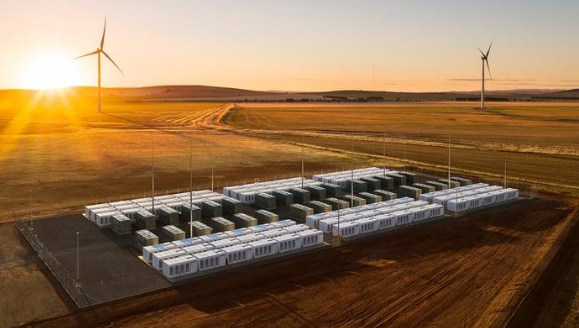
\includegraphics[width=5cm]{figures-Chp0/3-Reseau.png}
\end{minipage}\hfill   
\begin{minipage}[c]{0.35\textwidth}     
\captionof{figure}{Installation d'un centre de stockage d'énergie éolienne, par Tesla, en Autralie exploité par le groupe français Neoen [tiré de la \href{https://www.maisondelenergie.fr/sites/maisondelenergie.fr/files/batteries_1.pdf}{maison de l'énergie, batteries}]}
\label{tab:battery_reseau}
\end{minipage}

Bien entendu, à l'heure de la transition écologique, accompagnée du développement des énergies renouvelables, l'intégration des systèmes de stockage de masse au sein des réseaux électriques constitue un enjeu. En effet, les énergies renouvelables : photovoltaïque, éolien, nucléaire sont des sources d'énergies moins flexibles que le charbon ou le gaz. Les deux premières présentent une dépendance aux conditions environnementales quand la dernière présente une production constante. Au sein du réseau électrique, l'intégration de batteries, en général sodium-soufre, permet une meilleure maîtrise des pics ou déficits de tension électrique.

Dans notre cas, l'étude des batteries sera décomposée en trois temps. Dans un premier temps, des rappels des notions d'électricité et d'électrochimie seront faites que vous soyez capable d'appréhender l'analyse des batteries. Dans un second temps, vous vous intéresserez aux méthodes analytiques permettant de mesurer l'efficacité d'une batterie. Dans un dernier temps, vous caractérisez une batterie lithium et vérifierez son adéquation à un cahier des charges.

\objectif{
La liste ci-dessous décrit les compétences à acquérir durant ce TP.

~

\faBattery[0] Notions élémentaires : 
\begin{itemize}
    \item pile vs accumulateur \& batterie primaire vs secondaire ;
    \item oxydant vs réducteur \& oxydation vs réduction ;
    \item composante d'une cellule : électrodes, électrolyte, séparateur ;
    \item anode vs cathode \& conventions générateur/récepteur ;
    \item potentiels rédox, interpréter la spontaneité ou non d'une réaction électrochimique ;
    \item courant, tension, puissance électrique, rendement en charge et en énergie d'une cellule.
\end{itemize}

\faBattery[2] Comprendre comment caractériser l'efficacité d'une batterie.
\begin{itemize}
    \item Mesure de l'état d'une pile : SoC, DoD et SoH ;
    \item Utiliser et interpréter une courbe tension-temps dans le cadre d'un cycle de charge et décharge ;
    \item Utiliser les rendements de charge et de décharge afin de caractériser la charge et la décharge.
\end{itemize}

\faBattery[4] Savoir diagnostiquer les propriétés électrochimiques d'une batterie.
\begin{itemize}
    \item Comprendre que les performances d'une batterie ou accumulateur peuvent être caractérisées par la capacité électrique, la puissance délivrable et la cyclabilité de la pile ;
    \item Caractériser l'état de charge et de décharge d'une batterie : SoC \& DoD ;
    \item Caractériser l'état de santé d'une pile : SoH ;
    \item Identifier les sources d'hystérèses entre la charge et la décharge ;
    \item Comprendre et poser des hypothèses sur les sources de vieillissement d'une batterie.
\end{itemize}}

\newpage

\chapter{\faBattery[0] Notions élémentaires à usage dans les batteries}

Une batterie est un dispositif qui stocke de l'énergie sous forme chimique et qui le restitue sous forme d'énergie électrique. Lors de ce processus, deux espèces chimiques rédox, c'est-à-dire des espèces chimiques capables d'échanger un ou plusieurs électrons, réagissent ensemble. Cette réaction libère de l'énergie sous deux formes : 
\begin{itemize}
    \item un travail utile \textbf{W'} qui est le travail électrique ;
    \item une déperdition d'énergie, la chaleur \textbf{Q}, c'est-à-dire de l'énergie thermique.
\end{itemize}

\begin{minipage}[c]{0.65\textwidth}
\centering
\includegraphics[width=5cm]{figures-Chp0/4-FirstPrinciple.png}
\end{minipage}\hfill   
\begin{minipage}[c]{0.35\textwidth}     
\captionof{figure}{Représentation des flux reçus par une batterie.}
\label{tab:battery_W_Q}
\end{minipage}

La batterie est parfois à usage unique ou rechargeable. Ainsi, si la batterie est rechargeable, le travail électrique est soit reçu $W' > 0$ (charge) ou cédé $W' < 0$ (décharge). En son sein, des éléments résistifs imposent que la batterie perd nécessairement, que ça soit en charge ou décharge, une partie de son énergie sous forme thermique $Q < 0$.

Cette capacité à recevoir ou non du travail électrique permet de classifier les batteries en plusieurs catégories.

\section{Classification des générateurs électrochimiques}

\begin{figure}[H]
\begin{centering}
\subfloat[\label{fig:cir_gen}]{\includegraphics[height=3cm]{figures-Chp0/5-CircuitGen}}\subfloat[\label{fig:cir_gen_sch}]{\includegraphics[height=3cm]{figures-Chp0/5-CircuitGen-Sch}}\hfill\subfloat[\label{fig:cir_rec}]{\includegraphics[height=3cm]{figures-Chp0/5-CircuitRec}}\subfloat[\label{fig:cir_rec_sch}]{\includegraphics[height=3cm]{figures-Chp0/5-CircuitRec-Sch}}
\par\end{centering}
{\tiny{}\caption{{\small{} Fig. \ref{fig:cir_gen}) Représentation schématique d'une pile AAA alimentant d'une résistance et une diode électroluminescente rouge ; Fig. \ref{fig:cir_gen_sch}) Circuit électrique équivalent ; ig. \ref{fig:cir_rec}) Représentation schématique d'une pile AAA et d'une résistance alimentée par un générateur en mode DC ; Fig. \ref{fig:cir_rec_sch}) Circuit électrique équivalent.}}
}{\tiny\par}
\end{figure}%WARNING : mettre U_B pour la tension de la batterie

Les générateurs électrochimiques peuvent être classifiés en deux grandes catégories : 

\subsection{Dispositifs constitués d'une seule cellule électrochimique}

\paragraph*{La pile électrique} est un dispositif électrochimique qui génère de l'électricité en convertissant de l'énergie chimique en énergie électrique grâce à une réaction d'oxydoréduction. 

Du point de vue électrique, la pile est donc un \textbf{générateur électrique} dont la réaction d'oxydoréduction est \textbf{irréversible}. Seul le cas, illustré Fig. \ref{fig:cir_gen}/\ref{fig:cir_gen_sch} est possible.

\paragraph*{L'accumulateur} est un dispositif électrochimique qui génère (resp. reçoit) de l'électricité en convertissant de l'énergie chimique (resp. électrique) en énergie électrique (resp. chimique) grâce à une réaction d'oxydoréduction réversible. 

Du point de vue électrique, l'accumulateur est :
\begin{itemize}
\item un \textbf{générateur électrique} lorsqu'il se décharge ;
\item un \textbf{récepteur électrique} lorsqu'il se charge
\end{itemize}
dont la réaction d'oxydoréduction est \textbf{réversible}. Les deux cas, illustré Fig. \ref{fig:cir_gen}/\ref{fig:cir_gen_sch} \& \ref{fig:cir_rec}/\ref{fig:cir_rec_sch} sont possibles.

\subsection{Dispositifs constitués de plusieurs cellules électrochimiques}

\paragraph*{La batterie} est le nom donné à tout dispositif électrique résultant de la mise en série et/ou en parallèle de plusieurs piles ou accumulateurs. On les classe alors en deux catégories : 
\begin{enumerate}
    \item Primaire lorsque l'on a mis en série des piles ;
    \item Secondaire lorsqu'on l'on a mis en série des accumulateurs.
\end{enumerate}

Ainsi, tout générateur primaire ne peut être utilisé qu'une unique fois, et doit être jeté après utilisation. 

\section{Réactions électrochimiques}
Avant d'aborder la structure d'une batterie, il est important de remettre en place quelques termes de vocabulaire propre aux réactions électrochimiques.

\paragraph*{Oxydant/Réducteur}

Dans ce type de réaction, l'une des espèces cède des électrons, c'est le réducteur et l'autre en gagne, c'est l'oxydant. 
\begin{center}
    \begin{align*}
        \underbrace{\ce{Cu^{2+}}}_{oxydant} (aq) + \underbrace{\ce{Zn(s)}}_{réducteur} &= \ce{Cu (s)} + \ce{Zn^{2+} (aq)}
    \end{align*}
\end{center}

\exercice{
\Q \label{Q:1.1} Dans chacune des réactions suivantes, indiquer l'oxydant et le réducteur :
\begin{enumerate}
    \item \ce{Li (s) + H2O (l) = Li^+ (aq) + HO^- (aq) + \frac{1}{2} H2 (g)} ;
    \item \ce{PbO2 (s) + Pb (s) + 2 H2SO4 (aq) = 2PbSO4 (aq) + 2 H2O (l)}
\end{enumerate}}


\paragraph*{Oxydation/Réduction}

Afin de modéliser le flux d'électron, il est possible de décomposer l'équation de réaction en deux demi-équations rédox modélisant chacune une oxydation (le couple qui libère des électrons) et une réduction (le couple qui gagne des électrons).
\begin{center}
\begin{minipage}{0.4\textwidth}
\begin{align*}
    \ce{Cu^{2+} (aq) + 2e^- &= Cu (s)}\\
    \ce{Zn(s) &= Zn^{2+} (aq) + 2e^- } \\
    \hline
    \ce{Cu^{2+}(aq)  + Zn(s) &= Cu (s) + Zn^{2+} (aq)} 
\end{align*}
\end{minipage}    
\end{center}

\exercice{\Q En reprenant les équations de réaction \ref{Q:1.1}, indiquer la demi-équation rédox et si il s'agit de la modélisation d'une oxydation/réduction sachant que les couples rédox mis en jeux sont les suivants :
\begin{enumerate}
    \item \ce{Li^+ (aq)} / \ce{Li (s)} \& \ce{H2O (l)}/\ce{H2 (g)} ; 
    \item \ce{PbO2} (s) / \ce{Pb^{2+} (aq)} \& \ce{Pb^{2+}} (aq) / \ce{Pb (s)}%voir peut-être retirer SO42-
\end{enumerate}}


\subsection{Description d'une batterie}
La description que nous allons faire traite de manière indifférente les batteries primaires et secondaires. En ces termes, piles et accumulateurs porteront le nom générique de cellule.

Toute cellule est un dispositif composé de $\ldots$

\paragraph*{$\ldots$ deux électrodes} dont l'une sert à capter les électrons et l'autre sert à céder des électrons. Une cellule est, par conséquent, un \textbf{dipôle électrique orienté}.

%WARNING : image pour orienter le dispositif électrique.

Chaque électrode joue un rôle précis, et son nom vous informe sur le processus physico-chimique mis en jeu : 
\begin{minipage}[c]{0.65\textwidth}
\centering
\begin{tabular}{ccc}
\toprule
\textbf{Type d'électrode} & \textbf{anode} & \textbf{cathode}  \\
\midrule
Réaction électrochimique & oxydation & réduction \\
Générateur & $\ominus$ & $\oplus$ \\
Récepteur & $\oplus$ & $\ominus$ \\
\bottomrule
\end{tabular}
\end{minipage}\hfill   
\begin{minipage}[c]{0.35\textwidth}     
\captionof{figure}{Conventions de nom et d'orientation électrique d'un accumulateur.}
\label{tab:conventions}
\end{minipage}




Dans le cas d'une pile Daniell, pile galvanique aqueuse utilisant les couples \ce{Cu^{2+}(aq)}/\ce{Cu(s)} et \ce{Zn^{2+}(aq)}/\ce{Zn(s)}, le dispositif peut se présenter de la manière suivante :

\begin{minipage}[c]{0.65\textwidth}
\centering
\includegraphics[width=8cm]{figures-Chp0/6-Diode-Voltmeter.png}
\end{minipage}\hfill   
\begin{minipage}[c]{0.35\textwidth}     
\captionof{figure}{Pile Daniell réalisée à l'aide :}
\begin{itemize}
    \item d'une solution de sulfate de cuivre accompagné d'une plaque de cuivre (cathode) ;
    \item d'une solution de sulfate de zinc accompagné d'une plaque de zinc (anode) ;
\end{itemize}

L'ensemble est fermé d'une part par un pont salin contenant une solution de \ce{KNO3} concentrée et d'autre part par un circuit électrique fermé.
\label{fig:pileCuZn_Exp}
\end{minipage}


Schématiquement, le dispositif s'écrit comme : 
\begin{equation}
\oplus \quad \ce{Cu(s)} | \ce{Cu^{2+} (aq)}; \ce{SO_4^{2-} (aq)} | K^+ (aq), NO_3^- (aq) | \ce{Zn^{2+} {aq}}; \ce{SO_4^{2-} (aq)} | \ce{Zn(s)} \quad \ominus
\label{eq:pileCuZn}
\end{equation}

où les $|$ indiquent les interfaces entre les différentes phases.


%WARNING : retrouvver l'infos
\paragraph*{$\ldots$ solvant} Le solvant est l'espèce permettant solvatant les espèces électroactives et électrolytiques.

Dans la pile Daniell, le solvant est l'eau.

\paragraph*{$\ldots$ séparateur} En général, les cellules sont composées d'un séparateur qui est une membrane ou un pont qui permet de séparer \textbf{physiquement} et \textbf{spécifiquement} les espèces électroactives du compartiment anodique et cathodique. Ce séparateur obéit à deux contraintes : empêcher toute réaction parasite entre espèces électroactives, tout en assurant une bonne conductivité ionique d'espèces chimiques chargées, mais inertes chimiquement.

Dans la pile Daniell, le pont salin est le séparateur.

\paragraph*{$\ldots$ électrolyte} Afin de fermer le circuit électrique, au sein de la pile, le courant doit être conduit. Contrairement aux fils et électrodes, où le courant est assuré par les électrons, dans la solution et le séparateur, le courant est assuré par la \textbf{migration} des ions. C'est ce qu'on appelle l'\textbf{électrolyte}.

Celui-ci obéit à deux contraintes : 
\begin{enumerate}
    \item diminuer la résistivité des compartiments anodiques et cathodiques ;
    \item garantir le processus de migration au sein de la solution.
\end{enumerate}

En effet, la résistance à la conduction ionique est souvent l'une des principales sources de déperdition de l'énergie chimique en chaleur. C'est ce que, tout bon électrochimiste que vous êtes, appellera \textbf{la chute ohmique} (c'est-à-dire la déperdition d'énergie sous forme d'énergie thermique à cause de la loi d'Ohm). Le second point ne sera abordé qu'en cours d'électrochimie avec Alireza Ranjbari.

{\Large \faWarning } Parfois, l'électrolyte support peut-être une ou plusieurs espèces électroactives. Dans la pil Daniell présentée Fig. \ref{fig:pileCuZn_Exp}, c'est le cas.

\exercice{
Les batteries utilisées couramment dans les véhicules électriques, mais également dans d'autres applications comme les téléphones portables, sont de type lithium-ion. Elles présentent l'avantage d'avoir une très grande énergie massique, comprise entre 90 et \SI{180}{\watt\hour\per\kilo\gram}. De plus, ces batteries, même partiellement déchargées, délivrent toujours la même puissance, ce qui permet une utilisation dans les mêmes conditions, quel que soit le niveau de charge. Le principe général d'une batterie lithium-ion est basé sur l'échange réversible des ions lithium entre une électrode positive en oxyde métallique (\ce{MO2}) et une électrode négative en graphite qui va stocker les ions lithium pendant la charge :

~

\begin{minipage}[c]{0.65\textwidth}
\centering
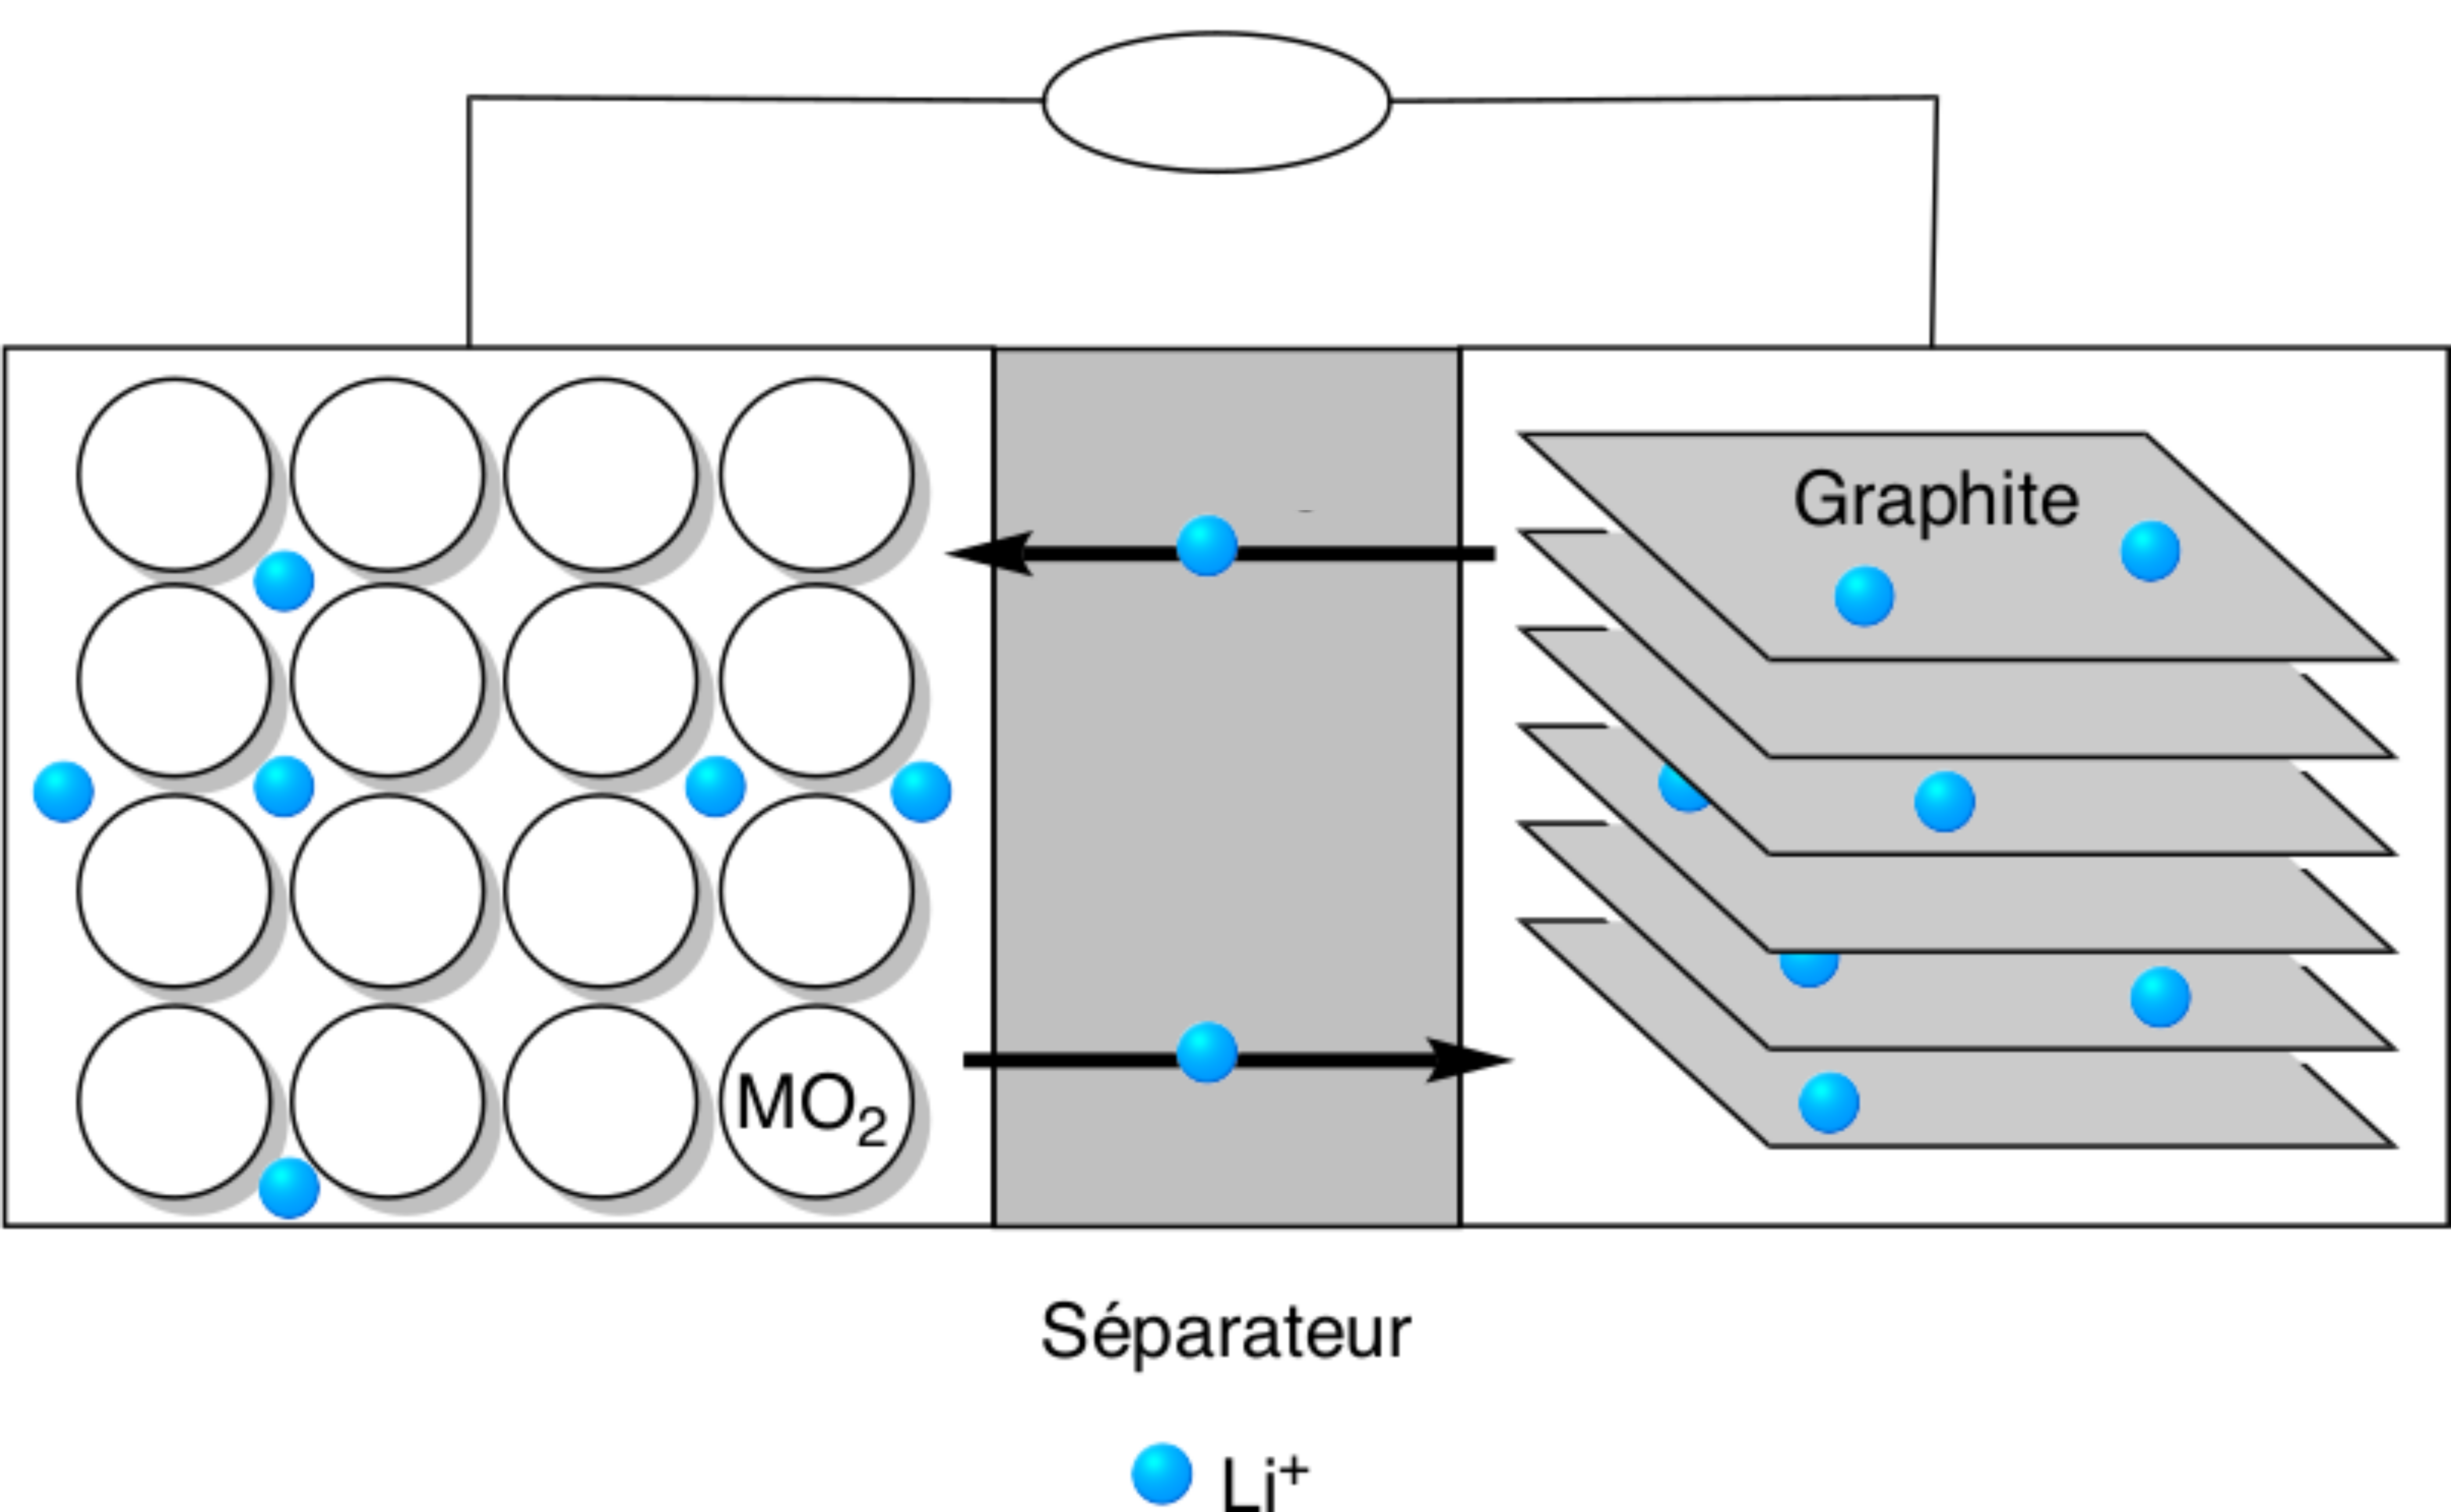
\includegraphics[width=6cm]{figures-Chp0/7-BatteryLithium.png}
\end{minipage}\hfill   
\begin{minipage}[c]{0.35\textwidth}     
\captionof{figure}{Technologie au lithium-ion. Le solvant utilisé est une espèce organique.}
\label{fig:li-ion}
\end{minipage}

\Q En vous appuyant sur la représentation du graphite, expliqué pourquoi les ions Li peuvent s'insérer entre les feuillets de graphite. On sait que le rayon ionique du lithium est de \SI{60}{\pico\meter} et le covalent est de \SI{134}{\pico\meter}.

\begin{minipage}[c]{0.65\textwidth}
\centering
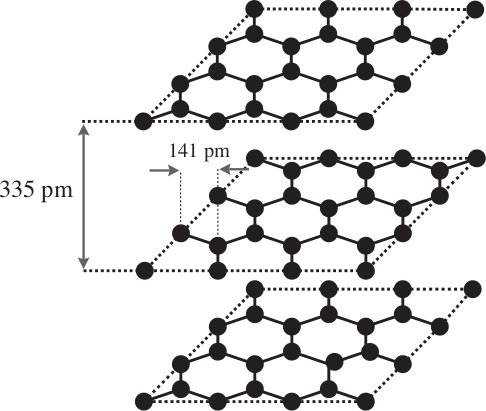
\includegraphics[height=4cm]{figures-Chp0/11-graphene.png}
\end{minipage}\hfill   
\begin{minipage}[c]{0.35\textwidth}     
\centering
\captionof{figure}{Structure du graphite}
\label{fig:graphite}
\end{minipage}

\Q A l'état totalement chargé, la structure du composé est \ce{LiC6}. Écrire la demi-équation rédox à cette électrode lors de la charge et de la décharge et préciser le signe de l'électrode de graphite.
La seconde électrode peut être en oxyde de cobalt (\ce{CoO2}) qui, après insertion des ions lithium,
forme l'oxyde lithié \ce{LiCoO2}. 
\Q Montrer que c'est l'élément cobalt qui change de degré d'oxydation ;
\Q Donner la demi-équation électronique associée au couple considéré lors de la charge et de la décharge
à cette électrode en précisant son signe.
\Q Reproduire et orienter le schéma de la Fig. \ref{fig:li-ion} dans le cas d'une charge puis d'une décharge. Vous indiquerez le nom et le signe des électrodes puis le flux d'électron, le courant électrique et la direction de migration des ions lithium.
%tiré de Mines-Pont 2022.

~

La suite de cet exercice sera traité à la partie suivante.}

\section{Caractériser un accumulateur ou une batterie}

\subsection{Charge, \'{E}nergie \& Puissance}
Les cellules électrochimiques sont des dispositifs électriques. Par conséquent, trois grandeurs électriques usuelles permettent de les caractériser : la charge (notée \textbf{C}), la tension (notée \textbf{U}) et le courant (notée \textbf{I}). Le courant dérive de la charge.

Deux grandeurs dérivées des trois grandeurs fondamentales de l'électricité peuvent nous intéresser :

\begin{enumerate}
    \item la puissance électrique instantannée, notée $P$
    \begin{equation}
        P(t) = U(t) I(t)
        \label{eq:puissance}
    \end{equation}
    \item le travail électrique, noté $W'$
    \begin{equation}
        W' = \int_0^t P(t') dt' = \int_0^t U(t') I(t') dt'
        \label{eq:travail}
    \end{equation}
\end{enumerate}

Lorsque le dispositif électrique est en convention récépteur (resp. générateur), la relation Eq.\ref{eq:puissance} nous donne la puissance \textbf{reçue} (resp. émie) par le dispositif. De même pour la relation sur le travail Eq.\ref{eq:travail}.

Bien entendu, toutes ces grandeurs sont à mettre en perspective avec la durée de vie d'un accumulateur. Tant qu'il présente une tension et une énergie stockée stable malgré les cycles de charge et de décharge, on peut considérer qu'il est fonctionnelle. Cette notion est appelée \textbf{cyclabilité}, c'est-à-dire le nombre de cycles de charge/décharge pendant lesquelles ces paramètres restent constants.

\exercice{
\Q Donner le signe de la puissance et du travail lorsqu'une cellule électrochimique est un récepteur reçoit de l'énergie. Même chose si il s'agit d'un générateur.

Dans les batteries, la puissance électrique est un critère de second plan. Ce qui intéresse principalement les industriels s'est que l'énergie délivrée par la batterie puisse stocker une grande quantité d'énergie, tout en la débitant de manière pérenne dans le temps.

\begin{center}
\begin{adjustbox}{width=0.95\textwidth}
\begin{tabular}{cccccc}
    \toprule
     \textbf{Technologie} & \textbf{Année de développement} & \textbf{Energie massique} & \textbf{Energie volumique} & \textbf{Tension} & \textbf{Cyclabilité}\\
     Unité & & \si{\watt\hour\per\kilo\gram} & \si{\watt\hour\per\liter} & \si{\volt}/au couple \ce{Li^+}/\ce{Li} & $\emptyset$ \\
     \midrule
     Plomb & 1859 & 35 & 70 & 2.0 & 200-250\\
     Nickel-Cadmium & 1900 & 60 & 100 & 1.2 & 400-500\\
     Nickel-Métal-Hydrure & 1975 & 80 & 240 & 1.2 & 400-500\\
     Lithium-Ion & 1978 & 250 & 400 & 3.6 & > 1000\\
     \bottomrule
\end{tabular}   
\end{adjustbox}
\captionof{table}{\small \'{E}volution des ordres de grandeurs de l'énergie massique, volumique, de la tension ainsi que de la cyclabilité d'une batterie en fonction de la technologie.}
\label{tab:battery_time}
\end{center}


\Q Commenter les valeurs de la Tab.\ref{tab:battery_time}. Quel est l'intérêt de la technologie Li-ion par rapport à d'autres technologies ?
\Q Mettre en relation ces données avec la place de l'élément Li au sein du tableau périodique.}



\subsection{État de charge et état de santé}
Afin de caractériser l'état d'une pile ou batterie, on peut utiliser diverses grandeurs caractéristiques permettant de définir son état à un instant $t$.

\paragraph*{\'{E}tat de charge (SoC, State-of-Charge)} L'état de charge d'une batterie indique la quantité d'énergie emmagasinée par la batterie. On la définit comme : 
\begin{equation*}
    SoC [\si{\percent}]= \frac{\text{charge emmaganisé par la batterie}}{\text{charge maximale que peut emmaganiser la batterie}} * 100
    \label{eq:SoC}
\end{equation*}

Si $SoC =$ \SI{0}{\percent} (resp. \SI{100}{\percent}), la batterie est déchargée (resp. chargée)


\paragraph*{\'{E}tat de décharge (DoD, Depth-of-Discharged)} L'état de décharge d'une batterie indique la quantité d'énergie non emmagasinée par la batterie. On la définit comme : 
\begin{equation*}
    DoD [\si{\percent}]= \frac{\text{charge non emmaganisé par la batterie}}{\text{charge maximale que peut emmaganiser la batterie}} * 100
    \label{eq:DoD}
\end{equation*}

Par définition, $DoD [\si{\percent}] = 100 - SoC [\si{\percent}]$. Si $DoD =$ \SI{0}{\percent} (resp. \SI{100}{\percent}), la batterie est chargée (resp. déchargée)

\paragraph*{\'{E}tat de santé (SoH, State-of-Health)} L'état de santé d'une batterie indique la charge maximale réelle par rapport à la charge maximale théorique que peut contenir la batterie.
\begin{equation*}
    SoH [\si{\percent}]= \frac{\text{charge maximale réelle}}{\text{charge maximale théorique}} * 100
    \label{eq:SoH}
\end{equation*}

L'état de santé permet de caractériser l'état de vieillissement de votre pile. Si la pile est neuve (resp. usagée), alors $SoH =$ \SI{100}{\percent} (resp. $SoH \to$ \SI{0}{\percent}).

\exercice{%sujet central 2022

Suite de l'exercice$\ldots$

\Q Déterminer l'expression de la capacité de la batterie (en \si{\ampere\hour\per\kilo\gram}) en fonction du nombre d'électrons échangés, de la constante de Faraday et de la masse molaire du matériau d'insertion (le graphite).

Pour le véhicule considéré, équipé d'une batterie lithium-ion dont les caractéristiques sont fournies dans le \textbf{Document}, la jauge d'autonomie de la batterie indique \SI{20}{\percent}. Son conducteur souhaite la recharger et pour cela, il utilise une borne de recharge qui fournit une puissance constante de \SI{7.40}{\kilo\watt} en délivrant un courant électrique d'intensité constante de \SI{32.0}{\ampere}.

\Q Calculer l'énergie massique maximale de la batterie considérée (\textbf{Document}). Commenter.

\Q Calculer l'énergie emmagasinée par la batterie lors de sa charge pour passer d'un SOC de \SI{20}{\percent}
à \SI{80}{\percent} et définir le rendement de la charge, puis le calculer. Commenter cette valeur.

Récemment, des chercheurs, en utilisant une anode composée de feuillets de graphène et de \ce{SnO2} sont parvenus à réaliser une batterie dont la capacité spécifique est de \SI{635}{\milli\ampere\hour\per\gram} après 100 cycles charge/décharge, la capacité spécifique étant à l'origine de \SI{784}{\milli\ampere\hour\per\gram}. La diminution de la capacité spécifique est liée à la grande surface spécifique du graphène et est due à la perte irréversible d'ions lithium, du fait de la décomposition de l'électrolyte, qui précipite et passive la surface de l'anode accessible pour la lithiation.

\Q Calculer l'état de santé de cette batterie.

\Q Estimer la perte de surface spécifique pour la batterie étudiée par les chercheurs.

~

\textbf{Document}

~

\emph{La technologie lithium-ion est communément utilisée dans les batteries des voitures électriques. Les principales caractéristiques d'une batterie Li-ion présente dans le véhicule électrique considéré dans
cette étude sont les suivantes :}

~

\begin{minipage}[c]{0.65\textwidth}
\centering
\begin{tabular}{cc}
     \'{E}nergie utilisable & \SI{41}{\kilo\watt\hour} \\
     Tension totale & \SI{400}{\volt} \\
     Nombre de cellules & 192 \\
     Masse de la batterie & \SI{305}{\kilo\gram} \\
\end{tabular}
\end{minipage}\hfill   
\begin{minipage}[c]{0.35\textwidth}     
    \captionof{table}{Principale caractéristique d'une batterie Li-ion d'un véhicule électrique.}
    \label{tab:li-ion_car}
\end{minipage}

~

\emph{Pour la batterie considérée, la variation SoC en fonction du temps de charge de la batterie est donnée à la figure suivante : }

~

\begin{minipage}[c]{0.65\textwidth}
\centering
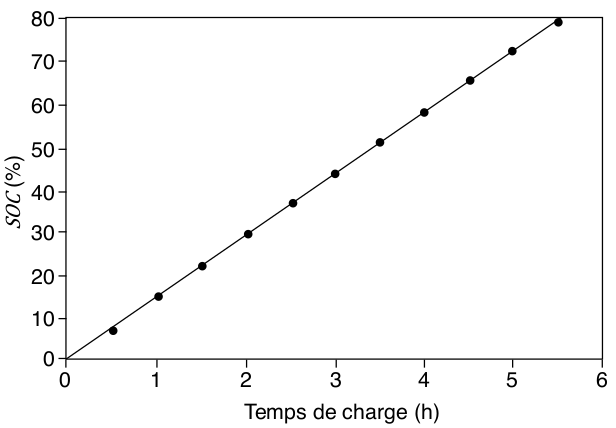
\includegraphics[width=6cm]{figures-Chp0/10-SoC.png}
\end{minipage}\hfill   
\begin{minipage}[c]{0.35\textwidth}     
    \captionof{figure}{\'{E}volution du SoC en fonction du temps de charge.}
    \label{fig:li-ion_car}
\end{minipage}
}

\appendix

\def \FigPath{/home/jeff/Documents/IUTOrsay/1-Cours/3p06-Cours_Batterie/01-Cours/figures-ChpAnn1/}
\graphicspath{{/home/jeff/Documents/IUTOrsay/1-Cours/3p06-Cours_Batterie/01-Cours/figures-ChpAnn1/}}
\normchapter{Rappels de thermodynamique}

L'objectif de cette annexe est de rappeler l'ensemble des notions (vocabulaire, définition, relations$\ldots$) de première année permettant de décrire un système thermodynamique et qui pourront intervenir en chimie des matériaux.

Pour la majorité d'entre vous, il est naturel pour vous de décrire l'état d'un système mécanique par sa position et sa vitesse et d'utiliser les lois de Newton pour décrire l'évolution d'un tel système. \`{A} chaque état du système, vous êtes en capacité de prédire n'importe quel grandeur : énergie, accélération$\ldots$

\begin{minipage}{0.45\textwidth}
\centering

\includegraphics[width=10cm]{Fig01.pdf}
\end{minipage} \hfill \begin{minipage}{0.45\textwidth}
\captionof{figure}{Démarche, niveau lycée, permettant l'étude d'un système mécanique.}
\label{fig:01}
\end{minipage}


%Les cellules électrochimiques (ou batteries) constituent des \textbf{systèmes thermodynamiques}. 
Par analogie avec la mécanique, l'état d'un système thermodynamique sera décrit par des \textbf{variables d'état}. L'évolution des systèmes thermodynamiques sera donnée, comme le font les lois de Newton en mécanique, par deux postulats fondamentaux appelés \textbf{principes de la thermodynamiques}.

\section{Description d'un systèmes thermodynamique}

Pour simplifier, nous considérerons un système thermodynamique, noté $\Sigma$, composé d'une phase unique isotrope et homogène (\emph{par ex.} un gaz dans un piston)

\subsection{\'{E}tat d'un système}

La thermodynamique est la science des échanges d'énergie (\emph{par ex.} les échanges thermiques) ou des échanges de matière.

\definition{
Pour caractériser la présence ou l'absence d'échange d'énergie ou de matière entre un système thermodynamique $\Sigma$ et l'extérieur, les adjectifs suivants sont utilisables : 

~

\begin{minipage}{0.5\textwidth}
\begin{tabular}{cccc}
\toprule
& Isolé & Fermé & Ouvert \\
\midrule
Echange d'énergie & \faRemove & \faCheck & \faCheck \\
Echange de matière & \faRemove & \faRemove &\faCheck \\
\bottomrule
\end{tabular}
\end{minipage}\begin{minipage}{0.5\textwidth}
\captionof{table}{Terme de vocabulaire à utiliser en présence ou absence de flux d'énergie ou de matière avec l'extérieur.}
\end{minipage}
}



\subsection{Variable d'état}
Les variables sont un N-uplet de grandeurs permettant de décrire l'état macroscopique d'un système, qui peuvent être de deux natures$\ldots$


\subsubsection{$\ldots$ extensives}

\definition{Une variable extensive est une variable $X$ qui dépend de la taille du système.

Si l’on réunit deux systèmes $\Sigma_1$ et $\Sigma_2$ identiques caractérisés par les valeurs $X_{\Sigma_1} = X_{\Sigma_2}$, la valeur de X pour le système $\Sigma_1 + \Sigma_2$ est :

\begin{equation}
X_{\Sigma_1 + \Sigma_2} = X_{\Sigma_1} + X_{\Sigma_2} = 2 X_{\Sigma_1} = 2 X_{\Sigma_2}
\end{equation}
}

Les grandeurs extensives communément rencontrées sont :
\begin{center}
\begin{tabular}{cccc}
\toprule
Nom & volume & quantité de matière & masse \\
\midrule
Symbole & $V$ & $n$ & $m$ \\
Unité SI & \si{\meter\cubed} & \si{\mole} & \si{\kilo\gram} \\
\bottomrule
\end{tabular}
\captionof{table}{Variables d'état extensives}
\end{center}

Les grandeurs extensives sont finalement des grandeurs qui dépendent directement de la quantité de matière.

%\exercice{

%\begin{center}
%
\includegraphics[width=5cm]{Fig01}
%\end{center}

%On considère deux recipients contenan chacun deux gaz différents noté $\Sigma_1$ et $\Sigma_2$, considérés comme parfait. Identifier les variables extensives chacun de ces systèmes. Un opérateur ouvre la vanne, de volume négligeable, entre les deux récipients. En déduire la valeur des paramètres extensifs du système $\Sigma_1 + \Sigma_2$.}

\subsubsection{$\ldots$ intensives}
\definition{Une variable intensive est une variable $Y$ qui ne dépend pas de la taille du système.

Si l’on réunit deux systèmes $\Sigma_1$ et $\Sigma_2$ identiques caractérisés par les valeurs $Y_{\Sigma_1} = Y_{\Sigma_2}$, la valeur de $Y$ pour le système $\Sigma_1 + \Sigma_2$ est :
\begin{equation}
Y_{\Sigma_1 + \Sigma_2} = Y_{\Sigma_1} = Y_{\Sigma_2}
\end{equation}
}

Les grandeurs intensives communément rencontrées sont :

\begin{minipage}{0.5\textwidth}
\centering
\begin{tabular}{ccc}
\toprule
Nom & température & pression \\
\midrule
Symbole & $T$ & $P$ \\
Unité SI & \si{\kelvin} & \si{\pascal} \\
\bottomrule
\end{tabular}
\end{minipage}\begin{minipage}{0.5\textwidth}
\captionof{table}{Variables d'état intensives}
\end{minipage}

\`{A} chaque grandeur intensive, il est possible d'associer une interprétation microscopique. La température permet de décrire l'agitation thermique des molécules à l'échelle microscopique. La pression permet de décrire les chocs des particules contre la paroi du système thermodynamique. %La force électromotrice permet de décrire la différence d'énergie potentielle électrique des particules chargées entre (deux phases.

%\exercice{Dans les deux gaz décrit précédemment, identifier les variables intensives. En déduire la valeur des paramètres intensifs du système $\Sigma_1 + \Sigma_2$.}

\subsection{Fonctions d'état}
Les fonctions d'état sont un ensemble de fonction qui dépendent des variable d'état et décrivent l'état du système. Ce sont ces fonctions qui seront soumises aux principes thermodynamiques permettant de décrire l'évolution du système.

Ces fonctions d'état, comme l'énergie en mécanique, ont pour propriété de ne pas dépendre du chemin thermodynamique mais uniquement de l'état initial et final d'une transformation.

\subsubsection{Entropie et ses grandeurs d'échanges}

L'entropie est une fonction d'état qui ne fait sens qu'à l'échelle macroscopique. C nom, d'origine allemande, dérive du terme grec \emph{entropê} qui signifie \og action de se transformer, changement \fg{}.

L'objet de cette grandeur est de traduire l'évolution irréversible d'un système thermodynamique isolé sous la forme d'une fonction mathématique. On peut assimiler à votre niveau l'entropie à la flèche du temps.

Pour cela, les anciens ont postulé que dans un système isolé, il existe une fonction d'état extensive appelée entropie qui ne peut que croître. Pour cela, il ont crée une grandeur d'échange appelée \og entropie de création \fg{} qui ne peut qu'être positive ou nulle, traduisant l'augmentation de l'entropie d'un système isolé.

\definition{L'entropie de création est une grandeur d'échange, notée $S_c$ et d'unité \si{\joule\per\kelvin}, qui traduit l'augmentation d'un système isolé : 

\begin{equation}
S_c \geq 0
\end{equation}

Deux cas de figure sont possibles,
\begin{align*}
S_c &= 0 \implies \text{l'évolution du système est réversible} \\
S_c &> 0 \implies \text{l'évolution du système est irréversible}
\end{align*}}

Cependant, les systèmes étudiés (comme les batteries) sont rarement isolés. Un système peut perdre de l'entropie, comme il peut perdre de la chaleur et donner son entropie à l'extérieur. On définit alors un nouvelle grandeur d'échange, définie dans l'ensemble des réels, traduisant l'échange d'entropie avec l'extérieur. 


\definition{
L'entropie de création est une grandeur d'échange, notée $S_e$ et d'unité \si{\joule\per\kelvin}, qui traduit l'échange d'entropie avec le reste de l'univers. Elle est liée à l'échange thermique par : 
\begin{equation}
S_e = \frac{Q}{T_{ext}}
\end{equation}

où $T_{ext}$ est la température de l'extérieur et $Q$ l'échange thermique.}


\subsubsection{\'{E}nergie interne}

Lorsqu'un système thermodynamique est considéré comme immobile dans un référentiel mécanique, on peut considérer que l'énergie du système est égale à l'énergie interne du système.

\definition{ 
L'énergie interne $U$ d'un système thermodynamique correspond à la somme des énergies cinétique, notée $e_c (micro)$ et potentielle d'interactions microscopiques , notée $e_p (micro)$ des particules constituant le système. On peut alors écrire que 

\begin{equation} 
U = e_c (micro) + e_p (micro)
\end{equation}

$U$ a la dimension d’une énergie et son unité $SI$ est le Joule.}

L'énergie interne est permet de rendre compte de toutes les intéractions au sein des structures moléculaires, à la fois intramoléculaire (liaison chimiques) ou intermoléculaires (van der Waals, liaison hydrogène$\ldots$).

\subsubsection{Enthalpie}
Dans la majorité des situations, le chimiste travaille avec des phases condensées et est peu intéressé par le travail des forces de pression. Afin de le négliger, le chimiste construit une nouvelle fonction chimique et la soustrait de l'énergie interne.


\definition{ 
L'enthalpie d’un système thermodynamique la fonction d’état :
\begin{equation}
H = U + PV
\end{equation}

où $U$ est l’énergie interne, $P$ la pression et $V$ le volume. L’enthalpie se mesure en joules.}

En supprimant les forces de pression, l'enthalpie ne rend compte que des interations moléculaires mises en jeu au sein du système.

\subsubsection{Enthalpie libre}
Nous verrons que cette grandeur est de la plus grande utilité en chimie. Il s'agit de l'enthalpie qui contient toutes les énergies autes que l'énergie des forces de pression, corrigée de l'énergie inutilisable par le système, d'origine entropique.

\definition{ 
L'enthalpie libre d’un système thermodynamique la fonction d’état :
\begin{equation}
G = H - TS
\end{equation}

où $H$ est l’enthalpie, $T$ la température et $S$ l'entropie. L’enthalpie se mesure en joule par kelvin.}


\subsubsection{Propriétés et bilan}

On peut résumer l'ensemble des fonctions d'état courantes en chimie dans le tableau \ref{tab:FonctionEtat}
%propriété
\begin{center}
\begin{tabular}{ccccc}
\toprule
Fonction d'état & énergie interne & entropie & enthalpie & enthalpie libre \\
\midrule
Définition & $U$ & $S$ & $H=U+PV$ & $G = H - TS$ \\
Unité & \si{\joule} & \si{\joule\per\kelvin} & \si{\joule} & \si{\joule} \\
\bottomrule
\end{tabular}
\captionof{table}{Bilan des fonctions d'état}
\label{tab:FonctionEtat}
\end{center}

Les fonctions d'état ont plusieurs propriétés mathématiques/physiques utiles : 

\begin{enumerate}
\item elles sont extensives, c'est-à-dire qu'elles dépendent de la taille du système ;

\begin{minipage}{0.5\textwidth}
\centering

\includegraphics[scale=0.4]{Fig04a}
\end{minipage}\begin{minipage}{0.5\textwidth}
\captionof{table}{Extensivité de l'énergie interne.}
\end{minipage}


\item elles sont additives, c'est-à-dire que si on considère deux systèmes thermodynamiques simultanément, leurs fonctions d'état s'additionnent.

\begin{minipage}{0.7\textwidth}
\centering

\includegraphics[scale=0.4]{Fig04b}
\end{minipage}\begin{minipage}{0.3\textwidth}
\captionof{table}{Additivité de l'énergie interne.}
\end{minipage}


\item la variation des fonctions d'état ne dépend que de l'état initial et final du système.

\begin{minipage}{0.5\textwidth}
\centering

\includegraphics[scale=0.4]{Fig04c}
\end{minipage}\begin{minipage}{0.45\textwidth}
\captionof{table}{La variation d'énergie interne reste inchangé entre les trois chemins thermodynamique du moment que l'état final et initial sont les mêmes.}
\end{minipage}

\end{enumerate}

La dernière propriété est très importante, c'est elle qui nous permet de construire des chemins thermodynamiques, parfois fictifs, pour remonter à la variation des fonctions d'état.


\section{Description d'une transformation thermodynamique}

\subsection{Grandeurs d'échange}

Les grandeurs d'échange permettent de caractériser l'échange d'énergie entre le système $\Sigma$ et l'extérieur à chaque instant d'une évolution. On les sépare en deux catégories en fonction de si oui ou non elles sont décrites exclusivement par la thermodynamique.

\definition{Le transfert thermique, aussi appelé chaleur et noté $Q$, caractérise l'échange d'énergie causé par une différence de température entre le système $\Sigma$ et l'extérieur.

En particulier, on qualifie d'adiabatique toute transformation où le transfert thermique ne s'établit pas. Habituellement, une transformation adiabatique s'établit lorsque ;
\begin{itemize}
\item la paroi du système empêche tout échange d'énergie thermique (on parle de paroi athermique ou calorifugée) ;
\item la transformation est suffisamment rapide pour que l'échange thermique ne puisse pas s'établir (\emph{par ex.} une explosion).
\end{itemize}

}

Les transferts thermiques sont intrinsèques à la thermodynamique et n'ont pas d'équivalence dans les autres branches de la physique.


Le travail est l'ensemble des transferts d'énergie qui en sont pas d'origine thermiques. 

\definition{
Un travail constamment présent est le travail mécanique causé par une différence de pression entre le système $\Sigma$ et l'extérieur.

Contrairement à la chaleur, le travail mécanique dispose d'une expression analytique donnée sous forme infinitésimale par : 

\begin{equation}
\delta W_P = - P_{ext} dV
\end{equation}

où $dV$ est la variation infinitésimale de volume du système $\Sigma$.}

Par exemple, si on considère un gaz extérieur, à la pression $P_{ext}$, qui comprime un second gaz dans un piston en appliquant une force extérieure $\vec{F}_{ext} = - F_{ext} \vec{e}_x$. Entre un temps $t$ et $t+dt$, le piston est comprimé d'une longueur $d\vec{l} = dx \vec{e}_x$.

\begin{minipage}{0.45\textwidth}
\centering

\includegraphics[scale=0.7]{Fig05}
\end{minipage} \hfill \begin{minipage}{0.45\textwidth}
\captionof{figure}{Compression d'un piston}
\end{minipage}

On sait que la force s'exprime comme 
\begin{align*}
F_{ext} = P_{ext} \cdot S
\end{align*}

avec $P_{ext}$ la pression extérieure et $S$ la surface du piston.

\begin{align*}
\delta W_P &= \vec{F}_{ext} \cdot d\vec{l} \\
&= - P_{ext} S dx \\
&= -P_{ext} dV
\end{align*}

avec $dV$ la variation infinitésimale du volume du piston.



\subsection{Type de transformations}

On notera $X_i$ (resp. $X_f$) une grandeur intensive initiale (resp. finale). 

 
\definition{
\textbf{Thermostat} se dit d'un système thermodynamique capable d'échanger de la chaleur avec un système $\Sigma$ et dont la température, notée $T_{ext}$, est constante.

~

\textbf{Barostat} se dit d'un système thermodynamique capable d'échanger du travail mécanique avec un système $\Sigma$ et dont la pression, notée $P_{ext}$, est constante.

~

\textbf{Isochore} se dit d'une transformation au cours de laquelle le volume V du système est constant.

~

\textbf{Monobare} se dit d'une transformation au cours de laquelle le système $\Sigma$ est soumis à une pression constante $P_{ext}$ de telle sorte qu'à l'état initial $P_i$ et à l'état final $P_f$, le système est à l'équilibre mécanique. Mathématiquement, ceci se traduit par : 
\begin{equation}
P_i = P_f = P_{ext}
\end{equation}

~

\textbf{Isobare} se dit d'une transformation au cours de laquelle le système $\Sigma$ est soumis à une pression constante $P_{ext}$ de telle sorte qu'à chaque instant, le système est à l'équilibre mécanique. Mathématiquement, ceci se traduit par : 
\begin{equation}
\forall t, \quad P = P_{ext}
\end{equation}

~

\textbf{Monotherme} se dit d'une transformation au cours de laquelle le système $\Sigma$ est soumis à une température constante $T_{ext}$ de telle sorte qu'à l'état initial $T_i$ et à l'état final $T_f$, le système est à l'équilibre thermique. Mathématiquement, ceci se traduit par : 
\begin{equation}
T_i = T_f = T_{ext}
\end{equation}

~

\textbf{Isotherme} se dit d'une transformation au cours de laquelle le système $\Sigma$ est soumis à une température constante $T_{ext}$ de telle sorte qu'à chaque instant, le système est à l'équilibre mécanique. Mathématiquement, ceci se traduit par : 
\begin{equation}
\forall t, \quad T = T_{ext}
\end{equation}
}

De toutes ces définitions, on en déduit que les transformations sont iso-X sont des cas particuliers des transformations mono-X.

%\exercice{Classer ces transformations dans chacune des catégories :
%\begin{itemize}
%\item 
%\end{itemize}}

\subsection{Condition d'équilibre}

L'équilibre thermodynamique correspond à l'état final du système thermodynamique. 

%En général, si on étudie un système isolé, l'équilibre peut être calculé en cherchant le maximum de l'entropie.

\subsubsection{\'{E}quilibre thermique}

Considèrons un système $\Sigma_1$ à la température $T_1$ mis en contact avec un système $\Sigma_2$ à la température $T_2$.

\begin{center}

\includegraphics[scale=0.7]{Fig03a}
\captionof{figure}{Mise en contact de deux gaz séparés par une paroi diatherme (qui laisse passer la chaleur) non movible}
\end{center}

On met en contact ces deux systèmes et on considère le système $\Sigma = \Sigma_1 + \Sigma_2$. Si ce système forme un système isolé, le système évoluera jusqu'à égalité des températures $T_1$ et $T_2$.

Dans le cas où ce système est en contact avec un thermostat, la température finale sera donnée par la température du thermostat.

\definition{\`{A} l'équilibre thermique entre un système $\Sigma_1$ et $\Sigma_2$, les températures sont égales : 
\begin{equation*}
T_1 = T_2
\end{equation*}

~

Si ces systèmes sont isolés ou subissent une transformation adiabatique, la température finale pourra être déterminée à l'aide du premier principe.

~

Si ces systèmes sont en contact avec un thermostat à la température $T_{ext}$, alors :
\begin{equation*}
T_{ext} = T_1 = T_2
\end{equation*}

}

\subsubsection{\'{E}quilibre mécanique}

Considèrons un système $\Sigma_1$ à la pression $P_1$ mis en contact avec un système $\Sigma_2$ à la température $P_2$.

\begin{center}

\includegraphics[scale=0.7]{Fig03b}
\captionof{figure}{Mise en contact de deux gaz séparés par une paroi  amovible}
\end{center}


On met en contact ces deux systèmes et on considère le système $\Sigma = \Sigma_1 + \Sigma_2$. Si ce système forme un système isolé ou thermostaté, le système évoluera jusqu'à égalité des pressions $P_1$ et $P_2$.

\definition{\`{A} l'équilibre mécanique entre un système $\Sigma_1$ et $\Sigma_2$, les pressions sont égales : 
\begin{equation*}
P_1 = P_2
\end{equation*}}

\section{Principes thermodynamiques}

\subsection{Premier principe}

\definition{
Il est postulé que dans un système isolé et immmobile (c'est-à-dire n'échangeant pas de matière, pas de travail et de charleur), l'énergie du système est conservée.}

La conséquence est que lorsque l'on considère un système fermé évoluant d'un état $A$ vers un état $B$, l'évolution du système est donnée par : 
\begin{align}
\Delta U &= U_B - U_A \\ 
&= Q_{A \to B} + W_{P,A \to B} + W'_{A \to B}
\end{align}

Si on considère que le système est la batterie qui évolue d'un état A à un état B, au contact de l'atmosphère (qui joue le rôle de barostat et thermostat), on trouve alors :

\begin{equation}
\Delta U = Q + W_P + W'
\end{equation}

Dans le cas d'une transformation infinitésimale du système, on peut écrire que : 

\begin{equation}
d U = \delta Q + \delta W_P + \delta W'
\end{equation}


Or le travail des forces de pression est un grandeur peut intéressante pour un chimiste, lequel souhaite utiliser une fonction d'état ne dépendant que de la chaleur reçue et du travail utile reçu. Pour cela, un chimiste est emmené à plutôt utiliser le premier principe à pression constante.


\definition{
Le premier principe à pression constante, c'est-à-dire pour un système en contact avec un barostat, s'écrit comme :
\begin{equation}
\Delta H = Q + W'
\end{equation}

Ce principe est valable au final pour toutes les transformations monobares, en général vérifié pour les systèmes chimiques.}

En particulier, dans une transformation adiabatique ($Q=0$), le travail utile $W'$ venant de l'extérieur est intégralement transformé en enthalpie (dans un système chimique, en énergie chimique). 

\example{
%\blanc{}
On considère une évolution d'un système thermodynamique $\Sigma$ soumis à un barostat. On peut alors écrire l'évolution de l'enthalpie comme :
\begin{align}
\Delta H &= \Delta (U +PV) \\
&= \Delta U + V \Delta P + P \Delta V \\
&=  Q + W_P + \delta W' + VdP + P dV \\
&=  Q + \delta W' + V \Delta P + (P-P_{ext}) \Delta V
\end{align} 

Si le système subit une transformation monobare, on a alors : 

\begin{align}
\Delta H = Q + W'
\end{align}

Si le système subit une transformation isobare, on peut étendre la relation ci-dessus aux transformations infinitésimales : 

\begin{align}
d H = \delta Q + \delta W'
\end{align}
}

\subsection{Second principe}

\definition{
La variation d'entropie de ce système contient deux termes, l'un associé à l'échange de chaleur avec l'extérieur (noté $S_e$) et l'autre associé à l'évolution naturelle du système si celui-ci était isolé (noté $S_c$). Au bilan, on a :

\begin{equation}
\Delta S = S_e + S_c
\end{equation}

Dans le cas d'une transformation infinitésimale, on peut écrire : 

\begin{equation}
d S = \delta S_e + \delta S_c
\end{equation}}

Lorsqu'un système est isolé et est tout au long de sa transformation à l'équilibre (thermique et mécanique), on dit que le système évolue de manière isentropique (isentropique = adiabatique + réversibilité).

Les systèmes chimiques sont le plus souvent en contact avec un barostat, mais aussi un thermostat, ce qui conduit à ce que les transformations chimiques soient le plus souvent monobares et monothermes. Dans ces transformations, l'enthalpie libre est la fonction pour permet de décrire l'évolution du système.

\definition{
L'évolution d'un système à pression et température constante est donnée par l'inégalité suivante :

\begin{equation}
\Delta G \leq W'
\end{equation}}

\example{
%\blanc{}
On considère une transformation d'un système thermodynamique $\Sigma$ en contact avec un thermostat et un barostat. On peut alors écrire la variation d'enthalpie libre comme :
\begin{align}
\Delta G &= \Delta (H - TS) \\
&= \Delta H - T \Delta S - S \Delta T \\
&=  Q + W' - T \Delta S - S \Delta T \\
&= T_{ext} S_e + W' - T \Delta S - S \Delta T \\
&= T_{ext} \Delta S - T_{ext} S_c + W' - T \Delta S - S \Delta T \\
&= -T_{ext} S_c + W' + (T_{ext} - T) \Delta S - S \Delta T \\
\end{align} 

Puisque le système subit une transformation monotherme, on a $T = T_{ext}$, ce qui se traduit par : 

\begin{align}
\Delta G = -T S_c + W'
\end{align}

On sait que par construction, $S_c \geq 0$ d'où $-T S_c \leq 0$, donc 

\begin{align}
\Delta G \leq W'
\end{align}

Si la transformation est isobare et isotherme, la relation ci-dessus est valable pour des transformations infinitésimales : 

\begin{align}
d G \leq \delta W'
\end{align}
}

Une façon intuitive de comprendre cette relation est la suivante : 


\begin{center}
\begin{tabular}{C{3cm}C{5cm}C{7cm}}
$\Delta G = W'$ & transformation réversible & le travail utile reçu par le système est entièrement converti en énergie utilisable \\
$\Delta G < W'$ & transformation irréversible & le travail utile reçu par le système est partiellement converti en énergie utilisable. Une partie est perdue.\\
\end{tabular}
\end{center}


\section{Grandeurs de réaction}

\subsection{Définition}
En chimie, vous savez que l'évolution d'une transformation chimique est décrite par l'avancement $\xi ~ [\si{\mole}]$. Afin de faire apparaître l'avancement, on a besoin d'introduire les grandeurs de réaction.

\definition{
La grandeur de réaction associée à une fonction d'état $X$ (X=U, H, S ou G) et notée $\Delta_r X$, est définie par :

\begin{equation}
\Delta_r X = \left ( \frac{\partial X}{\partial \xi} \large \right )_{T,P}
\end{equation}

Il s'agit donc de la dérivée (variation) de la fonction d'état X lorsque la température et la pression sont maintenues constantes.}

\subsection{Critère d'évolution}

L'évolution d'un système thermodynamique, subissant une transformation chimique, est donné par le second principe de la thermodynamique.

\`{A} pression et température constante, on a 
\begin{align*}
d G &< 0 \\
\Delta_r G \cdot d \xi &<0
\end{align*}

Du second principe, on a trois situations possibles : 

\begin{minipage}{0.45\textwidth}
\centering

\includegraphics[scale=0.7]{Fig06}
\end{minipage}\hfill\begin{minipage}{0.45\textwidth}
\captionof{figure}{Profil d'enthalpie libre à différent avancement d'une réaction.}
\end{minipage}

La pente de l'enthalpie libre en fonction de l'avancement (=grandeur de réaction) nous indique si la réaction évolue dans le sens direct ($\xi \nearrow$) ou dans le sens indirect. Lorsque la pente est nulle, on peut considèrer que le système chimique est à l'équilibre.

\begin{minipage}{0.45\textwidth}
\centering
\begin{tabular}{ccc}
\toprule
Signe de $\Delta_r G$ & Nom associé & Sens d'évolution \\
\midrule
$\Delta_r G < 0$ & exergonique &  sens direct \ce{->} \\
$\Delta_r G > 0$ & endergonique &  sens indirect \ce{<-} \\
$\Delta_r G = 0$ & endergonique &  sens indirect \ce{<-} \\
\bottomrule
\end{tabular}
\end{minipage}\hfill\begin{minipage}{0.45\textwidth}
\captionof{figure}{Résumé des différents signes de l'enthalpie libre de réaction.}
\end{minipage}

\subsection{Relation entre grandeurs de réaction}

\definition{
Dans un système en température et pression constante, on peut lier les grandeurs de réaction par la relation : 
\begin{equation}
\Delta_r G = \Delta_r H - T \Delta_r S
\end{equation}
}

Cette relation vient de la définition de G (voir Tab. \ref{tab:FonctionEtat}), que l'on dérive par rapport à l'avancement.

\subsection{Utilisation des réactions de formation}

En sciences physiques, l'énergie est une grandeur relative, c'est-à-dire qu'on peut calculer des variations d'énergie, mais jamais l'énergie de manière absolue.

Les chimistes donc posé un état de référence pour chaque constituant chimique qui sert de $0$ pour l'enthalpie. On peut alors calculer l'enthalpie de tous les constituants par rapport à cet état de référence.

\subsubsection{\'{E}tat standard de référence}

\definition{\`{A} une température $T$ et une pression $P^\circ = 1 ~ \si{\bar}$, un élèment chimique admet un état chimique de référence, généralement sont état thermodynamique le plus stable.}

Pour un solide cristallisé, l'état standard de référence est la variété allotropiquela plus stable. Par exemple, pour le carbone à \SI{298}{\kelvin}, il s'agit du graphite (et pas le diamant).

Pour un gaz, il s'agit d'un corps simple : la molécule diatomique la plus stble à \SI{298}{\kelvin}. Cela est le cas pour \ce{H} \ce{H2}, \ce{F} (\ce{F2}), \ce{N} (\ce{N2}), O (\ce{O2}).

\definition{Pour élèments chimiques dans leur état standard de référence, la convention pose que  : 
\begin{align*}
\Delta_f H^\circ = 0
\end{align*}}

\subsubsection{Réaction de formation}

Dans le cas des corps simples qui ne sont pas un état de référence ou les corps complexes (c.-à-d. constitué de plusieurs constituants chimiques), les réactions de formations sont tabulées.

\definition{On appelle réaction standard de formation d’une espèce chimique (corps complexe) à la température T, la réaction au cours de laquelle une mole de ce corps dans son état standard à la température T est formée à partir des corps simples qui le constituent, chacun étant pris dans son état standard de référence.}

On peut donner quelques exemples à \SI{298}{\kelvin} : 

\begin{itemize}
\item eau liquide :
\begin{align*}
\ce{\frac{1}{2} O2 (g) + H2(g) -> H2O (l)} \quad \Delta_f H^\circ (\ce{H2O},l) = -285.10 \si{\kilo\joule\per\mole}
\end{align*}

\item diamant :
\begin{align*}
\ce{C (graphite) -> C(diamant)} \quad \Delta_f H^\circ (\ce{C},\text{diamant}) =  1.92 \si{\kilo\joule\per\mole}
\end{align*}
\end{itemize}

\subsubsection{Loi de Hess}

\definition{On appelle loi de Hess, la loi permettant de calculer l'enthalpie standard de réaction de n'importe quelle réaction à partir des réactions de formation des constituants.

Si on considère une réaction de la forme :

\begin{equation*}
\ce{\nu_1 A_1 + \nu_2 A_2 + \ldots \nu_N A_N = 0} \quad \Delta_r H^\circ
\end{equation*}

avec $\nu_k > 0$ (resp. $\nu_k < 0$) si il s'agit d'un produit (resp. réactif).

La loi de Hess s'écrit alors : 

\begin{align*}
\Delta_r H^\circ = \sum_i \nu_i \Delta_f H^\circ (A_i)
\end{align*}}

Par exemple, dans le cas de la combustion du méthane, on a :

\begin{equation*}
\ce{CH4(g) + 2 O2(g) = CO2(g) + 2 H2O(l)}
\end{equation*}

L'enthalpie de Hess permet d'écrire : 
\begin{align*}
\Delta_r H^\circ = 2 \Delta_f H^\circ (\ce{H2O}, l) + \Delta_f H^\circ (\ce{CO2}, g) - \Delta_f H^\circ (\ce{CH4}, g)
\end{align*}

\subsection{Utilisation des grandeurs molaires}
\subsubsection{Définition des grandeurs molaires}
Il arrive assez souvent que l'on ait besoin des grandeurs molaires pour calculer des grandeurs de réaction. 

En particulier, l'entropie s'y porte bien puisque contairement à l'énergie, elle est définie de manière absolue . On ne sait pas la mesurer directement, mais on peut la déduire de l'étude des équilibres chimiques ou thermiques.

\definition{
L'entropie molaire standard d'une substance chimique $A_i$, est l'entropie pour \SI{1}{\mole} de cette substance pris à $P^\circ = 1$ et à une température $T$.

L'entropie molaire est notée $S^\circ_m (\ce{A_i})$ et est donnée en \si{\joule\per\mole\per\kelvin}.}

\subsubsection{Calcul d'une grandeur standard de réaction}

\definition{
L'entropie de réaction standard d'une transformation chimique, modélisée par une équation de réaction de la forme : 
\begin{equation*}
\ce{\nu_1 A_1 + \nu_2 A_2 + \ldots \nu_N A_N = 0} \quad \Delta_r S^\circ
\end{equation*}

avec $\nu_k > 0$ (resp. $\nu_k < 0$) si il s'agit d'un produit (resp. réactif).

est donnée par : 
\begin{align*}
\Delta_r S^\circ = \sum_i \nu_i S_{m}^\circ (A_i)
\end{align*}
}

Cette relation peut se démontrer à l'aide des identités thermodynamique qui seront abordées au Chap. \ref{chp:thermochimie}.



\def \FigPath{/home/jeff/Documents/IUTOrsay/1-Cours/3p06-Cours_Batterie/01-Cours/figures-ChpAnn2/}
\graphicspath{{/home/jeff/Documents/IUTOrsay/1-Cours/3p06-Cours_Batterie/01-Cours/figures-ChpAnn2/}}
\normchapter{Fonctions à plusieurs variables}

En physique-chimie, il est rare que l'on puisse décrire un système avec une seule variable. En mécanique, on sait que l'énergie mécanique d'une particule est décrite par ses coordonnées spatiales et ses vitesses, soit 6 variables $(x,y,z,v_x, v_y, v_z)$. Il en est de même en thermodynamique, l'énergie interne par exemple est décrite canoniquement par trois variables $(S, V, N)$ (entropie, volume et nombre de particules).

Pour décrire ces systèmes, il est bien d'avoir quelques notions mathématiques sur les fonctions à plusieurs variables.

\section{Rappel sur la notation différentielle}

\definition{
Soit $f$ une fonction définie et continue au voisinage d'un point $x_0$. Cette fonction admet une dérivée, notée $f'$, telle que : 

\begin{align*}
f'(x_0) = \lim_{\Delta x \to 0} \frac{f(x_0 + \Delta x) - f(x_0) }{\Delta x}
\end{align*}

Si $f$ admet cette limite en $x_0$, on dit que $f$ est dérivable.}

En chimie, on note la dérivée différemment, puisqu'on écrit : 
\begin{equation}
f'(x) = \frac{df}{dx} (x)
\end{equation}

En général, la majorité des chimistes ne feront aucune distinction entre écrire $\frac{df}{dx} (x)$ (l'évaluation de la fonction dérivée au point x, c'est donc un nombre !) et $\frac{df}{dx}$ (la fonction dérivée, c'est un objet mathématique). Ce raccourci est fait par confort, car il permet de facilement passer de la dérivée, à la différentielle ! 

\definition{
\setlength{\columnsep}{5pt}
\begin{wrapfigure}{r}{0cm}% r à droite et l pour à gauche

\includegraphics[width=5cm]{Fig03}
\end{wrapfigure}

On appelle différentielle de $f$, la variation de la fonction $f$, notée $df$, entre un point $x$ et un point $x+dx$ infiniment proche. On note alors : 

\begin{align*}
df (x) = \frac{f(x+dx) - f(x) }{dx} = \frac{df}{dx} (x) dx
\end{align*}

On retrouve dans cette notation les idées de la définition mathématique.}


\section{Dérivées partielles}

Dès à présent, on posera $f$ une fonction à deux variables $(x,y)$ et $g$ une fonction à une variable $z$, on notera leur évaluation respective : 
\begin{align*}
x \to f'(x,y) \quad z \to g(z)
\end{align*}

En particulier, on verra en thermodynamique que les variables d'état dérivent des dérivées de fonctions à plusieurs variables. 

\definition{La dérivée partielle de la fonction $f$ par rapport à x au point (x,y) est la dérivée de la fonction d'une seule variable réelle : 
\begin{align*}
x \to f(x, y) \text{ où  y est constant}
\end{align*}

On note la fonction dérivée partielle : 
\begin{align*}
\left( \frac{\partial f}{\partial x} \right)_y \quad \frac{\partial f}{\partial x}
\end{align*}

La fonction $f$ est dites dérivable selon x au point (x,y), si la fonction $f$ est continue selon x au point (x,y). On peut alors écrire : 

\begin{equation*}
\frac{\partial f}{\partial x} (x,y)  = \lim_{\Delta x \to 0} \frac{f(x + \Delta x, y) - f(x, y)}{\Delta x}
\end{equation*}

On peut faire de même pour la dérivée partielle selon y.
}

Chaque dérivée a un sens bien précis : 

\begin{center}
\begin{tabular}{cC{12cm}}
$\left( \frac{\partial f}{\partial x} \right)_y$ & la dérivée partielle de $f$ par rapport à $x$ quand $y$ est constant \\
$\left( \frac{\partial^2 f}{\partial x^2} \right)_y$ & la dérivée partielle seconde de $f$ par rapport à $x$ quand $y$ est constant \\
$\left( \frac{\partial^2 f}{\partial x \partial y} \right)_y$ & la dérivée partielle de $f$ par rapport à $y$ quand $x$ est constant, suivie de la dérivée partielle par rapport à $x$ lorsque $y$ est constant
\end{tabular}
\end{center}

Les dérivées partielle seconde ne sont que la réalisation successive de deux dérivées partielle : 

\begin{align*}
\left( \frac{\partial^2 f}{\partial x^2} \right)_y &= \left( \frac{\partial}{\partial x} \left( \frac{\partial f}{\partial x} \right)_y \right)_y \\
\left( \frac{\partial^2 f}{\partial x \partial y} \right)_y &= \left( \frac{\partial}{\partial x} \left( \frac{\partial f}{\partial y} \right)_x \right)_y
\end{align*}

Au total, pour une fonction à 2 variables, on peut écrire $2$ dérivées premières et $4$ dérivées secondes : 
\begin{align*}
\left( \frac{\partial f}{\partial x} \right)_y & \left( \frac{\partial f}{\partial y} \right)_x & \left( \frac{\partial^2 f}{\partial x^2} \right)_y & \frac{\partial^2 f}{\partial x \partial y} & \frac{\partial^2 f}{\partial y \partial x} & \left( \frac{\partial^2 f}{\partial y^2} \right)_x
\end{align*}

\exercice{
Soit un gaz parfait dans une enceinte fermée. La loi des gaz parfait s'écrit : 
\begin{equation}
P(V,T) = \frac{nRT}{V}
\end{equation}

où $R$ est la constante des gaz parfait.

\Q Calculer les dérivées partielles premières.
%\begin{align*}
%\frac{\partial P}{\partial V} &= -\frac{RT}{V^2} \\
%\frac{\partial P}{\partial T} &= -\frac{R}{V}
%\end{align*}

\Q Calculer les dérivées partielles secondes.

}



\section{Différentielle totale exacte}
\subsection{Définition}

Dans les fonctions univariées, on sait qu'une fonction g(x) admet systématiquement une différentielle dg, à condition que la fonction $g$ soit dérivable : 
\begin{align*}
dg = \frac{dg}{dx} dx
\end{align*}

Ainsi, à chaque forme différentielle, on peut associer une fonction (c.-à-d. qu'une forme différentielle possède plusieurs primitives dont l'une de ces primitives correspond à g).

Dans les fonctions multivariées, il se trouve que tout ça se complique. On peut très bien définir la forme différentielle d'une fonction à deux variables :

\definition{
On appelle forme différentielle, toute expression mathématique d'une quantité $\delta f$, pouvant s'écrire : 
\begin{align*}
\delta f = X(x,y) dx + Y(x,y) dy
\end{align*}
où $X$ et $Y$ sont deux fonctions quelconques de $x$ et $y$.

Il est à noter que $\delta f$ est une petite quantité, qui peut avoir un sens physique, mais elle n'admet pas forcément de fonction primitive.
}

Le principal souci des formes différentielles, c'est qu'il n'existe pas forcément de fonction (de primitive) à une forme différentielle donnée. Par conséquent, on dit qu'une différentielle est totale exacte lorsqu'elle possède une primitive.

%Soit $f$ une fonction 
%$\Delta x = x - a$ et $\Delta y = y - b$

%\begin{align*}
%\Delta f &= f(x,y) - f(a,b) \\
%&= \frac{\partial f}{\partial x} (x,b) \Delta x + \frac{\partial f}{\partial y} (a,y) \Delta y
%\end{align*}

\exercice{Montrer si les fonctions suivantes admettent une forme différentielle et évaluer-là : 
\Q $f(x,y) = xy$
\Q $f(x,y) = (x-a)^2 + (y-b)^2$

~

Montrer si les formes différentielles suivantes sont exactes : 
\Q $\delta h = 6xy dx + 3x^2 dy$
\Q $\delta w = y^2 dx + x^2 dy$
\Q $\delta z = x^2 y^3 dx +3x^2 y^2 dy$}

\definition{La différentielle totale exacte d'une fonction $f$ à deux variables est définie comme : 
\begin{align*}
df = \frac{\partial f}{\partial x} dx + \frac{\partial f}{\partial y} dy
\end{align*}

On indique par $d$, au lieu de $\delta$, la différentielle lorsqu'elle est exacte.

Si une fonction admet une différentielle totale exacte, alors cette fonction est appelée \textbf{fonction d'état}.}

Une conséquence importante est que lorsque l'on intègre une fonction d'état entre un point initial et un point final, la valeur de son intégrale \textbf{ne dépend pas} du chemin suivi !

\subsection{Conséquence sur les différentielles croisées}

\definition{Une fonction d'état admet une égalité, appelée \textbf{égalité de Schwartz}, entre ses dérivées partielles croisées : 
\begin{align*}
\frac{\partial^2 f}{\partial x \partial y} = \frac{\partial^2 f}{\partial y \partial x}
\end{align*}}

Par conséquent, la réciproque vous indique que si une fonction suit l'égalité de Schwartz, alors cette fonction est une fonction d'état ! 

\exercice{\'{E}crire l'égalité de Schwartz des différentielles totales exactes suivantes : 
\Q $dU (S, V) = T(S,V) dS - P(S, V) dV$
\Q $dH (S, P) = T(S,P) dS + V(S,P) dP$ 
\Q $dG (T, P) = -S(T,P) dT + V(T,P) dP$

~

Montrer si les formes différentielles suivantes sont totales exactes. Conclure si la valeur de l'intégration dépend du chemin suivi.
\Q $\delta f = 6 x y^3 dx + 9x^2y^2 dy$
\Q $\delta g = x^2dx + xydy $}

\subsection{Intégration}
En thermodynamique, on est souvent emmené à décrire des transformations plutôt que des états, c'est-à-dire que mathématiquement, on exprime la variation d'une grandeur au lieu de sa valeur.

Dans les fonctions multivariées, toute la difficulté d'intégrer est inhérente au fait qu'il existe une infinité de chemins d'intégration. 

\begin{center}

\includegraphics[width=0.8\textwidth]{Fig02}
\end{center}

En effet, sur la figure ci-dessus représentant une fonction quelconque, on voit qu'il existe plusieurs façons d'intégrer d'un point $A$ à un point $B$. L'intégrale de cette fonction ne dépendra pas du chemin suivi si elle est une fonction d'état.

Cette idée de fonction d'état est simple à comprendre si on s'appuie sur un analogie à la vie courante. Imaginons que vous cherchiez cet hiver à aller à Bourg-Saint-Maurice en partant de Paris. D'un côté, pour faire la route, vous avez besoin de connaître le denivellé et d'un autre côté, vous avez besoin de connaître la distance. 

Peu importe la route que vous ferez, la différence d'altitude entre Bourg-Saint-Maurice et Paris sera toujours la même, vous aurez toujours le même dénivelé positif. Par contre, la distance, elle, dépendra du chemin que vous suivrez. Ainsi, le dénivelé est une fonction d'état, contrairement à la distance.


\definition{
Si f est une fonction d'état, elle admet donc une différentielle totale exacte. L'intégrale de $f$ d'un point $A$ à un point $B$ est unique et donne : 
\begin{equation*}
\int_A^B df = f_B - f_A
\end{equation*}}

Lorsque l'on connait la forme intégrale d'une fonction d'état, on peut trouver la valeur de son intégrale entre deux ponts en évaluant la fonction d'état en ces deux points. 

Malgré tout, il est bien de savoir intégrer une forme différentielle, en particulier, si l'on ne connait pas sa forme intégrale. Prenons par exemple la forme différentielle :
\begin{equation*}
\delta V = 2 \pi r h dr + \pi r^2 dh
\end{equation*}

Cette fonction respecte l'égalité de Schwartz : 
\begin{align*}
\frac{\partial^2 V}{\partial r \partial h} = \frac{\partial^2 V}{\partial h \partial r} = 2 \pi r
\end{align*}

On peut donc conclure que cette forme différentielle est totale exacte, soit :  
\begin{equation*}
d V = 2 \pi r h dr + \pi r^2 dh
\end{equation*}

On sait exprimer les dérivées partielles, prenons celle par rapport à $r$ : 
\begin{align*}
\frac{\partial V}{\partial r} = 2 \pi r h \stackrel{\text{integration}}{\implies} V({\color{blue} r}, h) &= V({\color{red} r_0}, h) + \int_{\color{red} r_0}^{r \color{blue}}  2\pi r' h dr'\\
&= V({\color{red} r_0}, h) + \pi ({\color{blue} r}^2-{\color{red} r_0}^2) h
\end{align*}

Quand on intègre, la constante d'intégration $V({\color{red} r_0}, h)$ n'est plus qu'une fonction de $h$, que l'on peut estimer à l'aide d'une autre dérivée partielle :

\begin{align*}
\frac{\partial V}{\partial h} (r_0, h)  = \pi r_0^2 \stackrel{\text{integration}}{\implies} V(r_0, h) = V(r_0, h_0) + \pi r_0^2 (h - h_0)
\end{align*}

On peut alors en déduire que : 
\begin{align*}
V (r, h) = \pi (r^2-r_0^2) h + \pi r_0^2 (h - h_0) + V(r_0, h_0)
\end{align*}

En particulier, pour $(r_0, h_0) = 0$, on retrouve $V(r,h) = \pi r^2 h$, ce qui correspond au volume d'un cylindre !  

\exercice{Soit les fonctions d'état suivantes. Intégrez-les de deux façons différentes entre le repère (donc le point (0,0) ou (0,0,0)) et un point M (a,b) ou M (a,b,c) où $(a,b,c)$ sont trois réels positifs.

\Q $S(r, h) = 2 \pi r h + 2 \pi r^2$
 
\Q $V(x,y,z) = x y z$}



\subsection{Recherche des extremums}

\setlength{\columnsep}{1pt}
\begin{wrapfigure}{r}{0cm}% r à droite et l pour à gauche

\includegraphics[width=5.0cm]{Fig01}
\captionof{figure}{Fonction $f(x,y) = (x-x_0)^2 + (y-y_0)^2$ près de son minimum}
\end{wrapfigure}

Dans une fonction à une variable, la ou les racines de sa dérivée nous donne ses extremums (maximum, minimum). Ainsi, si $g$ est dérivable, alors : 
\begin{align*}
\frac{dg}{dx} (x=x^\star) = 0 \implies (x^\star, g(x^\star))\text{ est la coordonnée d'un extremum de g}
\end{align*}

De la même manière, dans une fonction à plusieurs variables, partiellement dérivable selon x et selon y, on a : 
\begin{align*}
df (x^\star, y^\star) = \frac{\partial f}{\partial x} (x^\star, y^\star) \cdot dx + \frac{\partial f}{\partial y} (x^\star, y^\star) \cdot dy = 0 \implies (x^\star, y^\star)\text{ est un extremum de f}
\end{align*}

Dans les derivées à plusieurs variables, un extremum peut être un maximum, un minimum ou un point-selle.

\definition{
Soit $f$ une fonction partiellement dérivable selon x et selon y. Si x, y sont \textbf{indépendants} alors : 

\begin{align*}
df(x^\star, y^\star) = 0 \implies \frac{\partial f}{\partial x} (x^\star, y^\star) = 0 \textbf{ et } \frac{\partial f}{\partial y} (x^\star, y^\star) = 0
\end{align*}

Pour rechercher les extremums d'une telle fonction, il faut que les deux dérivées partielles soient nulles au point étudié !
}

Vous ne pouvez pas conclure sur le fait qu'un point soit un extremum sans étudier toutes les dérivées premières d'une fonction multivariée.

\def \FigPath{/home/jeff/Documents/IUTOrsay/1-Cours/3p06-Cours_Batterie/01-Cours/figures-ChpAnn3/}
\graphicspath{{/home/jeff/Documents/IUTOrsay/1-Cours/3p06-Cours_Batterie/01-Cours/figures-ChpAnn3/}}
\chapter{Théorie du champ cristallin}
\label{chp:cristal_field}
Une première théorie pour décrire les propriétés des complexes, appelée théorie du champ cristallin, fut énoncée en 1929 par H. Bethe et H. Van Vleck. Il s'agit d'un modèle électrostatique dans lequel les ligands sont considérés comme des sphères dures chargées négativement dont l'agencement dans l'espace perturbe la structure électronique de l'ion métallique libre en considérant uniquement les orbitales $d$ de valence, les autres étant trop basses en énergie. Plusieurs conséquences découlent donc de ces hypothèses :
\begin{itemize}
\item La structure électronique du complexe dépend de sa géométrie ;
\item Il n’y a pas de mise en commun des électrons du métal et du ligand : on considère une liaison purement ionique.
\end{itemize}


\section{Construction de la théorie pour la géométrie octaédrique}

\begin{center}

\includegraphics[width=0.8\textwidth]{Fig01}
\captionof{figure}{Représentation d'un isocontour des $5$ orbitales $d$. Les couleurs indiquent les 2 phases d'une orbitale.}
\end{center}

Si on considère un atome, métal, n'ayant aucune interaction avec son environnement, les 5 orbitales $d$ sont dégénérés. Maintenant, si on plonge le métal dans un "bain" d'électron, puisque la densité électronique autour du métal est uniforme et isotrope, la répulsion des électrons du métal-électrons du bain conduit une déstabilisation uniforme. Les orbitales $d$ sont déstabilisées d'une même valeur d'énergie $\Delta E$.


\begin{center}

\includegraphics[width=0.8\textwidth]{Fig02}
\captionof{figure}{Variation d'énergie des orbitales $d$ d'un métal plongé dans un environnement électronique sphérique (champ sphérique ou uniforme), puis dans un environnement électronique octaédrique (champ octaédrique)}
\end{center}

Si on considère maintenant une géométrie octaédrique, la répulsion des orbitales $d$ du métal se fera de manière plus forte sur les axes $+x, -x, +y, -y, +z, -z$, où se trouve chacun des six ligands. Par conséquent, dans un champ octaédrique, les orbitales $d_{x^2 - y^2}$ et $dz^2$ sont plus destabilisées que dans un champ uniforme. Au contraire, les orbitales $d_{xy}$, $d_{yz}$ et $d_{xz}$ sont stabilisées par rapport au champ uniforme.


\definition{
La théorie du champ cristallin est un modèle électrostatique qui prédit que les orbitales $d$ d'un complexe métallique \textbf{ne sont pas} dégénérées. Le modèle de division des orbitales $d$ dépend du champ cristallin, qui est déterminé par l'\textbf{arrangement} et le \textbf{type} de ligand.
}

\section{Règle du barycentre et paramètre du champ cristallisation}

\definition{
La \textbf{règle du barycentre} stipule que la somme des énergies des orbitales $d$ dans un champ cristallin donné est conservée par rapport au champ cristallin uniforme. Ainsi,
\begin{align*}
\sum_i E(d_i) = 0
\end{align*}

~

On appelle le \textbf{paramètre de champ cristallin} octaédrique, la différence d'énergie $\Delta_O$ entre les niveaux $e_g$ ($dz^2$, $d_{x^2 - y^2}$) et $t_{2g}$ ($d_{xy}$,$d_{yz}$,$d_{xz}$).}

Par conséquent, avec les deux conventions au-dessus, on a deux équations à deux inconnues : 
\begin{align*}
\begin{cases} 3E(t_{2g}) + 2 E(e_g) &= 0 \\
E(e_g) - E(t_{2g}) &= \Delta_O 
\end{cases} \implies \begin{cases} E(t_{2g}) &= -\frac{2}{5} \Delta_O \\
E(e_g) &= \frac{3}{5} \Delta_O
\end{cases}
\end{align*}


On peut alors compléter le diagramme d'un élément du bloc d en géométrie (coordinence) octaédrique :

\begin{figure}[H]
\begin{minipage}{0.55\textwidth}

\includegraphics[width=\textwidth]{Fig03}
\end{minipage}\hfill\begin{minipage}{0.40\textwidth}
\captionof{figure}{\'{E}clatement des orbitales $d$ dans un champ cristallin octaédrique, où sont indiquées les différences d'énergie par rapport à l'état de référence sphérique.}
\end{minipage}
\end{figure}

\section{Autres géométries}

Une autre géométrie que l'on rencontrera souvent est la géométrie tétraédrique, où l'éclatement des orbitales est moindre (la distance ligand-métal est plus grande que dans un octaèdre équivalent) et inversé (ce sont les orbitales $t_2$ qui pointent vers les ligands).

\begin{center}

\includegraphics[width=0.8\textwidth]{Fig04}
\captionof{figure}{\'{E}clatement des orbitales $d$ dans la géométrie tétraédrique}
\end{center}

\`{A} cause de considérations purement géométriques, il existe une relation simple entre le paramètre de cristallin tétraédrique $\Delta_t$ et l'octaédrique $\Delta_O$ : 
\begin{align*}
\Delta_t = \frac{4}{9} \Delta_O
\end{align*}

Il est préférable de bien connaître le champ cristallin de ces deux géométries car tous les autres champs cristallins peuvent se déduire de celles-ci : 
\begin{center}

\includegraphics[width=0.8\textwidth]{Fig05}
\captionof{figure}{Quelques champs cristallins communs}
\end{center}

\section{Energie de stabilisation du champ cristallin (ESCC) et configuration électronique}
\definition{
L'\textbf{énergie de stabilisation du champ cristallin (ESCC)} est la différence d'énergie entre les électrons $d$ dans le champ cristallin réel par rapport aux électrons dans le champ sphérique.

~

La comparaison de deux ESCC permet de \textbf{comparer deux configurations électroniques} ou de \textbf{comparer deux géométries}, et d'identifier la plus stable (celle avec la plus petite ESCC).
}

Prenons par exemple l'atome \ce{Cr^{2+}} de configuration $d^4$. Celui-ci admet deux configurations possibles, représentées aux Fig. \ref{fig:06a} et \ref{fig:06b}, qui sont $(t_{2g})^4(e_g)^0$ et $(t_{2g})^3(e_g)^1$.

\begin{figure}[H]
\begin{minipage}{0.45\textwidth}
\subfloat[\label{fig:06a}]{
\includegraphics[width=4cm]{Fig06a}}\subfloat[\label{fig:06b}]{
\includegraphics[width=4cm]{Fig06b}}
\end{minipage}\hfill\begin{minipage}{0.50\textwidth}
\caption{Remplissage électronique pour un ion $d^4$ dans une \ref{fig:06a} configuration champ fort / bas spin ; \ref{fig:06b} configuration champ faible / haut spin.}
\end{minipage}
\end{figure}

L'énergie de stabilisation du champ cristallin permet de comparer ces deux configurations électroniques, qui dépendent de deux termes : 
\begin{enumerate}
\item le \textbf{coût énergétique} pour \textbf{apparier} deux électrons, appelé \textbf{énergie d'appariement} et notée $P$ ;
\item l'\textbf{éclatement} $\Delta_O$ entre les niveaux $e_g$ et $t_{2g}$.
\end{enumerate}

Calculons l'ESCC dans chacune des configurations : 
\begin{align*}
ESCC_a &= -4 \times \frac{2}{5} \Delta_O + P = -1.6 \Delta_O + P \\
ESCC_b &= -3 \times \frac{2}{5} \Delta_O + \frac{3}{5} \Delta_O = -0.6 \Delta_O 
\end{align*}

On a alors $\Delta ESCC = ESCC_b - ESCC_a = \Delta_O - P$, on en déduit alors deux situations possibles :
\begin{enumerate}
\item si $\Delta_O > P$, $ESCC_b > ESCC_a$, on parle alors de configuration "\textbf{champ fort}" ou "\textbf{bas spin}" ;
\item sinon, on parle de configuration "\textbf{champ faible}" ou "\textbf{haut spin}".
\end{enumerate}

\section{Paramètres influençant $\Delta_O$ et $P$}
On pourra retenir que le \textbf{paramètre de champ cristallin} $\Delta_O$ est influencé par : 
\begin{itemize}
\item la \textbf{nature du ligand} : il est difficile de rationaliser les tendances dans le cas des ligands, en général, plus l'atome lié au métal est "petit" et chargé (orbitales peu diffuses, forte densité électronique), plus $\Delta_O$ est grand. On a donc en général pour $\Delta_O$ : 

\begin{align*}
\ce{I^-}  < S^{2-}  < F^- < O^{2-}
\end{align*}

Il existe une série expérimentale, appelée \textbf{série spectrochimique} qui classe les ligands en fonction de la force du champ cristallin crée par sur un métal.

\item la \textbf{nature du métal} : plus le métal est diffus (vers la gauche et le bas dans le tableau périodique), plus $\Delta_O$ est grand ;
\item la \textbf{charge du métal} : plus le métal est chargé (degré d'oxydation élevé), plus $\Delta_O$ est grand.
\end{itemize}

Pour l'\textbf{énergie d'appariement}, on pourra retenir que l'énergie diminue lorsque les \textbf{orbitales} du métal sont plus \textbf{diffuses}. Par exemple, on aura : 
\begin{equation}
P( 3d ) > P( 4d ) > P( 5d )
\end{equation}


\definition{Au bilan, la théorie du champ cristallin permet par un approche intuitive pour décrire les comportements des complexes de métaux de transition des structures \textbf{ioniques}. Cependant, le modèle part du principe que l'on destabilise une structure en ajoutant un champ de ligand. Dans ce cas, d'où vient la stabilisation ? Bien entendu, que se passe-t-il si la liaison est \textbf{iono-covalente} avec une part non négligeable de \textbf{covalence} ? Il existe d'autres théories, plus complexes et abordées dans la suite de vos études, mais qui ne seront pas nécessaires au sein de ce module.}
\end{document}
